\documentclass[10pt]{book}
\usepackage[fontsize=9pt]{scrextend}
\usepackage[a5paper,top=26mm,bottom=20mm]{geometry}
\usepackage{mathpazo} % font style
\usepackage{gensymb} % extra symbols including degree
\usepackage{textcomp} %enables midtilde
\newcommand{\textapprox}{\raisebox{0.5ex}{\texttildelow}} %enables midtilde
\linespread{1.05} % Palatino needs more leading (space between lines)
\renewcommand{\familydefault}{\sfdefault}
%\usepackage{array,booktabs,arydshln,xcolor} %Allow creation of box in chapter9. Has to be loaded first, because of clash with tabulary
\usepackage{array,booktabs,arydshln} %Allow creation of box in chapter9. Has to be loaded first, because of clash with tabulary

\usepackage[utf8]{inputenc} % allow direct utf8 input
\usepackage[font=small,labelfont=bf]{caption} % make figure captions smaller and label bold
\usepackage{graphicx} % allow figures
\usepackage{hyperref} % allow hyperlinks
\usepackage{alltt} % allow soft-TT environment
\renewcommand{\ttdefault}{qcr} % set TT font to qcr which can be bolded
\usepackage{moresize} % adds intermediate font size used to make TT section fit nicer
\usepackage{varwidth} % make it easier to center text in overpic enviroment
\usepackage[anythingbreaks]{breakurl} % break urls to fit on page
\usepackage{rotating} % allow rotating of e.g. tables
\usepackage{tabulary} % allows tables to automatically adjust to line width
\usepackage{bm,amsmath} % deal with formulas and math
\usepackage{fancyhdr} % nice headers and footers
\usepackage{footnote} % enables to samve footnotes
  \fancypagestyle{plain}{% redefine the plain style, needed to preserve layout on chapter headings with fncychap
    \fancyhf{}
    \fancyhead[LE]{\leftmark}
    \fancyhead[RO]{\rightmark}
    \fancyfoot[LE,RO]{\thepage}
  }
\usepackage[toc,page]{appendix} % allow nice appendix
\usepackage[dvipsnames,table]{xcolor} % allow table cell colors
  \definecolor{deepcyan}{RGB}{47,99,84}
\definecolor{deepyellow}{RGB}{254,227,68}
\definecolor{deeporange}{RGB}{0,100,0} %DarkGreen http://instant-eyedropper.com/info/html_color_code/
\usepackage{tabularx} % for rare tables that refuse layout by regular means
\usepackage[percent]{overpic} % put text on top of figure, used for back
\usepackage{wrapfig} % text around figure for cv
\usepackage{watermark} % used for making the thumb indices
\usepackage[most]{tcolorbox} % nice rounded color text box
\usepackage{hyperref} % for label-url style hyperlinks
\usepackage{caption} % allow changing the font of captions, ie. make smaller when absolutely needed
\usepackage[nottoc]{tocbibind} % show bibliography in TOC
\usepackage[Glenn]{fncychap} % nicer looking chapter headings
  \ChNameVar{\Huge\fontfamily{lmss}\selectfont\color{black}}
  \ChNumVar{\Huge\fontfamily{lmss}\selectfont\color{black}}
  \ChTitleVar{\Huge\bfseries\fontfamily{lmss}\selectfont\color{deeporange}}
  \ChNameAsIs
  \ChTitleAsIs
  % defaults: \ChNameVar{\bfseries\Large\sf}, \ChNumVar{\Huge}, \ChTitleVar{\bfseries\Large\rm}, ChRuleWidth{1pt}, \ChNameUpperCase, \ChTitleUpperCase
\usepackage{atbegshi}% http://ctan.org/pkg/atbegshi
  \AtBeginDocument{\AtBeginShipoutNext{\AtBeginShipoutDiscard}}
\usepackage{float} %Allow better placement of floats (tables and figures)
\usepackage{subcaption} %Allows multiple images in one figure
\captionsetup[subfigure]{justification=justified,singlelinecheck=false} % Set justification of subfigure caption to the left of figure
% bibliography reference check:
%\usepackage{refcheck} % warn about unused references, also adds bibliography labels, disable for production
% plus:
%\nocite{*} % nocite will add ?..? to bibliography label when an entry is unused
%\bibliography{references}{}

\newcommand\VRule[1][\arrayrulewidth]{\vrule width #1} %Allow creation of box in chapter9 Combines with \usepackage{array,booktabs,arydshln} % load required packages
\raggedbottom % prevent spreading out paragraphs with lots of whitespace inbetween

\begin{document}

\pagestyle{empty}

\newgeometry{left=-0.50cm,right=-0.50cm,top=0cm,bottom=0cm,centering}
\includegraphics[width=\textwidth,height=0.99999\textheight,keepaspectratio]{img/frontcover}
\restoregeometry
\cleardoublepage

\setcounter{page}{1}

\clearpage
\newgeometry{left=-0.50cm,right=-0.50cm,top=0cm,bottom=0cm,centering}
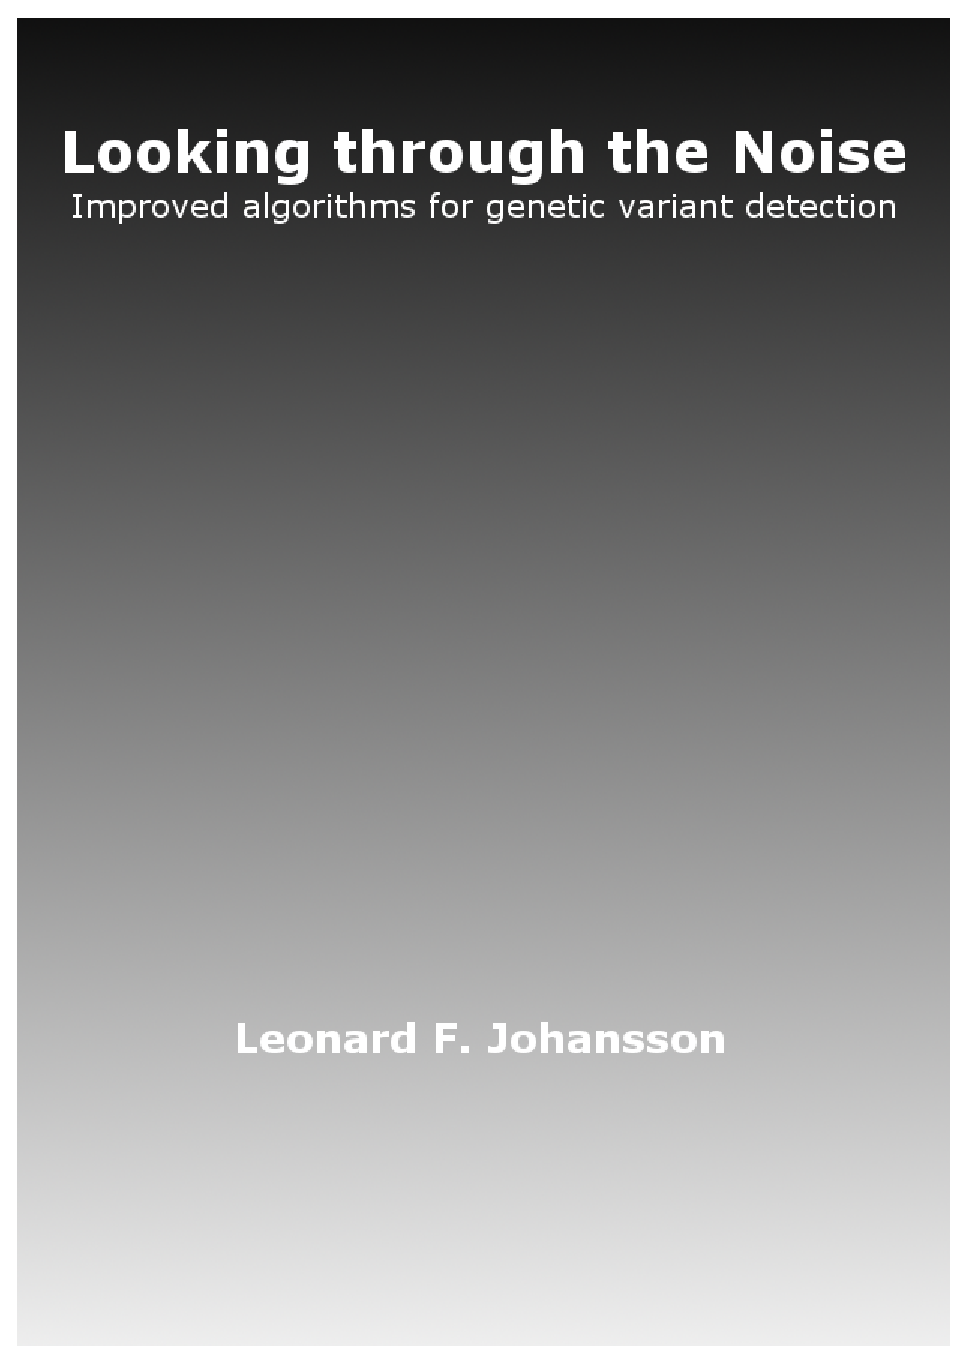
\includegraphics[width=0.935\textwidth,height=1.0\textheight]{img/frontcover_zw}
\restoregeometry
\clearpage

{\small
	\noindent
	Leonard Fredericus Johansson. \textbf{Looking through the noise: improved algorithms for genetic variant detection.} Thesis, University of Groningen, with summary in English and Dutch.
	\\~\\
	The research presented in this thesis was mainly performed at the Department of Genetics, University Medical Center Groningen, University of Groningen, Groningen, the Netherlands. Part of the work in this thesis was financially supported by ZONMW, grant no 40-41200-98-9159, Netherlands CardioVascular Research Initiative (CVON2011–19; Genius), and the Netherlands Organization or Scientific Research (NOW) VIDI grant number 917.164.455 received by Morris A. Swertz. 
	\\~\\
	Printing of this thesis was financially supported by Rijksuniversiteit Groningen, University Medical Center Groningen. 
	\\~\\
	Cover design and layout by L.F. Johansson.
	The front cover shows a variant that can only be seen when looking through the noise created by the four DNA nucleotides A, C, G and T. 
	\\~\\
	Printed by Ipskamp Drukkers, Enschede.\\
	\\
	© 2019 L.F. Johansson. All rights reserved. No part of this book may be reproduced or transmitted in any form or by any means without permission of the author.\\
	\\
	ISBN: XXX-XX-XXX-XXXX-X \mbox{~~~~~} ISBN (electronic version): XXX-XX-XXX-XXXX-X
}

\begin{figure}[!htbp]
	\centering
	
	\begin{minipage}[b]{0.24\textwidth}
		
\includegraphics[width=\textwidth]{img/colofon_umcg_zw}
	\end{minipage}
	\hfill
	\begin{minipage}[b]{0.29\textwidth}
		\raisebox{0.4\height}{
\includegraphics[width=\textwidth]{img/colofon_rug_zw}}
	\end{minipage}
	
\end{figure}

\clearpage

\begin{flushleft}
	
\includegraphics[scale=0.8]{img/rugr_logoen_zwart_rgb}
\end{flushleft}

\begin{center}
	\linespread{1.00} % squish slightly to fit everyone on page
	~\\
	\huge
	\textbf{Looking through the noise}
	\\~\\
	\large
	improved algorithms for genetic variant detection
	\\~\\
	\linespread{1.05} % and back to normal
	
	
	\large
	\textbf{PhD thesis}
	\\~\\
	\normalsize
	to obtain the degree of PhD at the\\
	University of Groningen\\
	on the authority of the\\
	Rector Magnificus prof. C. Wijmenga\\
	and in accordance with \\
	the decision by the College of Deans.
	\\~\\
	This thesis will be defended in public on
	\\~\\
	Wednesday 25 September 2019 om 12.45 hours 
	\\~\\~\\
	by
	\\~\\~\\
	\large
	\textbf{Leonard Fredericus Johansson}
	\\~\\
	\normalsize
	born on 29 May 1980\\
	in Hefshuizen\\
	\normalsize
\end{center}

\clearpage

\noindent
\textbf{Supervisors}\\
Prof. R.H. Sijmons \\
Prof. M.A. Swertz \\

\noindent
\textbf{Co-supervisor}\\
Dr. B. Sikkema-Raddatz \\

\noindent
\textbf{Assessment Committee}\\
Prof. V.V.A.M. Knoers\\
Prof. M. Vihinen\\
Prof. J.K. Ploos van Amstel\\


\clearpage

\noindent
\textbf{Paranymphs}\\
E.N. de Boer\\
K.K. van Dijk-Bos\\

\clearpage
\null\newpage

\noindent
	\Large
Propositions

\small

\begin{enumerate}
	
	\item Depending on how samples are prepared and analyzed, next-generation sequencing is suitable for detection of both base-level variants and structural variants. \textsl{(this thesis)}
	
	\item High coverage next-generation sequencing data is suitable for single-exon copy number variation detection. \textsl{(this thesis)}
	
	\item Before biological variability can be detected in next-generation sequencing, first laboratory induced variability has to be minimalized \textsl{(this thesis)}
	
	\item International screening program criteria  are currently not fully met for opportunistic genetic screening.\textsl{(this thesis)}
	
	\item In non-invasive prenatal testing, the use of multiple independent models increases the reliability of  the prediction of presence of a trisomy from a single data set. \textsl{(this thesis)}
	
	\item The same measurement outcome in non-invasive prenatal testing gives different results for women with different prior risks of carrying a child with a trisomy. \textsl{(this thesis)}
	
	\item Noise is everything that, from a certain perspective, blocks the path between reality and measurement outcome. \textsl{(this thesis)}
	
	\item Data can be of high and low quality at the same time (depending on what information should be retrieved from the data). \textsl{(this thesis)}
	
	\item Understanding how or why is seldom as useful as understanding that things are. \textsl{(Robin Hobb, Fool's Assassin)}
	
	\item It’s not what you look at that matters, it’s what you see. \textsl{(Henry David Thoreau)}
	
\end{enumerate}

\clearpage


 \makeatletter %Next three lines added to create double lines in the table of contends in case of long titles
	\def\@pnumwidth{3em}
\makeatother

\tableofcontents

\pagestyle{fancy}
\fancyhf{}
\fancyhead[LE]{\leftmark}
\fancyhead[RO]{\rightmark}
\fancyfoot[LE,RO]{\thepage}

\chapter{Introduction}
\label{chap:introduction}

{ \Large \leftwatermark{
\put(-76.5,-75){
\includegraphics[scale=0.8]{img/thumbindex.eps}}  \put(-67,-66.5){ {\color{white} 1 }}
\put(-67,-91.5){ 2 }
\put(-67,-116.5){ 3 }
\put(-67,-141.5){ 4 }
\put(-67,-166.5){ 5 }
\put(-67,-191.5){ 6 }
\put(-67,-216.5){ 7 }
\put(-67,-241.5){ 8 }
\put(-67,-266.5){ 9 }
\put(-67,-291.5){ 10 }
\put(-67,-316.5){ 11 }
} \rightwatermark{
\put(346.5,-75){
\includegraphics[scale=0.8]{img/thumbindex.eps}}  \put(350.5,-66.5){ {\color{white} 1 }}
\put(350.5,-91.5){ 2 }
\put(350.5,-116.5){ 3 }
\put(350.5,-141.5){ 4 }
\put(350.5,-166.5){ 5 }
\put(350.5,-191.5){ 6 }
\put(350.5,-216.5){ 7 }
\put(350.5,-241.5){ 8 }
\put(350.5,-266.5){ 9 }
\put(350.5,-291.5){ 10 }
\put(350.5,-316.5){ 11 }
}}

\newpage

\section{A short history on chromosomes and DNA} \label{intro_history}
In 1865 the Augustinian friar and scientist Gregor Mendel was the first to give a systematic account of the heredity of traits following specific laws \cite{Mendel_1866}. 
In the following decades it was discovered that during cell division a substance in the cell nucleus, dubbed \textsl{chromatin} (stainable substance) by German biologist Walther Flemming, was divided over the two halves of the cells during a process that Flemming called \textsl{mitosen}, or mitosis \cite{Schneider_1873,Flemming_1882,Cremer_2006}. 
A few years later, in 1890, German histologist Richard Altmann noted the presence of granules in cells that he believed were elementary organisms enclosed within cells, features later renamed ‘mitochondria’ by German microbiologist Carl Benda \cite{Altmann_1894,Benda_1898}. 
In 1888, German anatomist Wilhelm Waldeyer was the first to use the term \textsl{chromosomen} – chromosomes, meaning colored bodies – to describe the individual pieces of chromatin thread \cite{Waldeyer_1888,Cremer_2006}. 
In the last decade of the 19th century, the German biologist August Weismann proposed that the chromosomes were the bearers of hereditary material, which he called \textsl{keimplasma}, or germ plasm \cite{Weismann_1892}. 
At the time he was unaware of Mendel’s work. However, after its rediscovery at the turn of the century, the cytologists Walter Sutton, from the United States of America, and Theodor Boveri, from Germany, both showed that chromosomes follow Mendelian laws \cite{Sutton_1902,Boveri_1904,Boveri_1909,Crow_2002}. 

The chromosome theory of heredity quickly became the leading theory in the field that became known as genetics, a term introduced by the English biologist William Bateson in 1905 \cite{Keynes_2008}. 
Around the same time, he and his colleagues observed coupling between different traits in pea plants \cite{Bateson_1906,Lobo_2008}, leading the British biologist Thomas Morgan, upon further \textsl{Drosophila} studies, to state that ‘we find “associations of factors” that are located near together in the chromosomes’ \cite{Morgan_1911}. 
This led to the theory of linkage a few years later \cite{Morgan_1915}. 
It was several more decades before the normal human chromosome number was correctly defined as 46 by Indonesian cytogeneticist Joe Hin Tjio in 1956 \cite{Tjio_1956}. 
After that it took only a few more years, until 1959, for French scientists Lejeune, Gauthier and Turpin to connect Down syndrome to the presence of a small extra chromosome \cite{Lejeune_1959}.
One year later, the Philadelphia-based researchers Hungerford and Nowell discovered a small abnormal chromosome present in people with human chronic myelogenous leukemia, demonstrating the use of cytogenic techniques in diagnosis of hematological diseases \cite{Nowell_1960}. 
This chromosome was later named the ‘Philadelphia chromosome’ and shown to be the product of translocation between chromosomes 9 and 22 \cite{Rowley_1973}.

In the meantime, based on work by British physicist Maurice Wilkins and chemist Rosalind Franklin, American biologist James Watson and British physicist Francis Crick created the double-helix DNA model containing the four nucleotides – Adenine, Cytosine, Guanine and Thymine – which are paired A=T and G$\equiv$C \cite{Watson_1953,Wilkins_1953,Franklin_1953}. 
Several years later Crick and his team inferred – without being able to sequence – the triplet DNA-protein translation code \cite{Crick_1961,Yanofsky_2007}. 
However, it was not until the following decade, when British Chemist Frederick Sanger invented DNA sequencing methods, that the DNA sequence itself could be read \cite{Sanger_1975,Sanger_1977}. 
In 1963, it was discovered that apart from the nucleus, mitochondria also contained DNA \cite{Nass_1963}. 
In 1983, Huntington’s disease was the first human disease to be linked to a specific genomic marker \cite{Gusella_1983}. 
In the following years more diseases were linked to genomic markers and genetic diagnostics expanded from analysis of chromosomes to inclusion of DNA analysis. 
After the invention of Polymerase Chain Reaction (PCR), DNA analysis became much easier \cite{Saiki_1985,Saiki_1988} and at the turn of the 21st century scientists were able to create a draft sequence of the human genome \cite{Lander_2001,Venter_2001}. 

The introduction of so-called next-generation sequencing in 2005 ushered in the start of yet another era \cite{Mardis_2013}. 
Sequencing costs decreased rapidly to the point that a whole genome can now be sequenced for less than 1000 dollars \cite{Goodwin_2016}, opening up new possibilities for human genome analysis and bringing the fields of cytogenetics and molecular genetics closer together\footnote{Paragraph 1.1 suggests a logical and continuous timeline between discoveries. However, many of those discoveries were heavily contested and others were made by several research groups independently around the same time. This means that the history told in this paragraph could just as well have contained other names. Their omission is not meant to discredit their scientific contribution, but this introduction is too short to give a more nuanced vision of the scientific progress in genetics.}. 



\section{Human genome variation} \label{intro_variation}
With improving genomic analysis techniques came increasing knowledge about the composition of the human genome. 
When comparing any two individuals, their six billion base pair human genome will show many differences, or DNA variants. On average, everyone has around three million DNA variants that differ from the major allele present in the population, of which 10.000-11.000 are non-synonymous variants that change the triplet code and result in an amino-acid change of a protein \cite{Durbin_2010}. 
Most of those variations do not cause disease but, as will be discussed in section 1.6, some variants are associated with or can contribute to a congenital disorder or a predisposition for the development of a disease. 

Several types of DNA variants can be distinguished. The smallest are Single Nucleotide Variants (SNVs) and indels: insertions or deletions of one or more bases (Figure \ref{fig:Introduction_Fig1}A-D). 
When a larger stretch of DNA is lost or duplicated, the variant is considered to be structural variation (SV) and the term Copy Number Variation (CNV) is used (Figure \ref{fig:Introduction_Fig1}E-H). 
The size threshold to distinguish a large indel from a small CNV is arbitrary, and different definitions are used in literature. While 1 kb was traditionally used as the lower threshold for CNVs, variants larger than 50 bp are now labelled as CNVs \cite{Redon_2006,Tan_2014,Wilfert_2017}. 
In formal notation, duplication is regarded as a tandem duplication, i.e. insertion of a duplicate sequence, following directly 3’of the original copy (figure \ref{fig:Introduction_Fig1}F), leaving the formal term ‘insertions’ to signify all other nucleotide insertions \cite{den_Dunnen_2016} (Figure \ref{fig:Introduction_Fig1}D and H). 
However, in practice, the term duplication is used in a broader sense for copy number gains that can also include translocational insertions \cite{Kang_2010,Hanemaaijer_2012}. 
One subset of duplications is repeat expansions in which a repeated nucleotide sequence is extended. 
An example of this is the CAG repeat that is extended in Huntington disease \cite{Rubinsztein_1996}. 
Another type of SV are translocations, in which terminal parts of chromosomes are exchanged (figure \ref{fig:Introduction_Fig1}I). 
In reciprocal translocations both derivative chromosomes are present without an apparent net loss or gain of chromosomal content, but in so-called unbalanced translocations, the translocation results in loss of part of one chromosome and gain of part of another chromosome \cite{Maithripala_2017}. 
In Robertsonian translocations, two acrocentric chromosomes are connected at the centromere \cite{Robertson_1916} (Figure \ref{fig:Introduction_Fig1}J). 
A further type of DNA variation are inversions in which a nucleotide sequence is replaced by its reverse complement sequence \cite{Sudmant_2015,den_Dunnen_2016} (Figure \ref{fig:Introduction_Fig1}K). 
While reciprocal translocations and inversions are balanced events in principle, deletions or insertions are often present around the breakpoints in both types of variations \cite{Sudmant_2015,Simioni_2017}. 
A further type of chromosomal variation are aneuploidies, in which whole chromosomes are lost or gained (and can be considered as whole chromosome CNVs), such as in Down syndrome (Figure \ref{fig:Introduction_Fig1}L).  


\begin{figure}[!ht]
	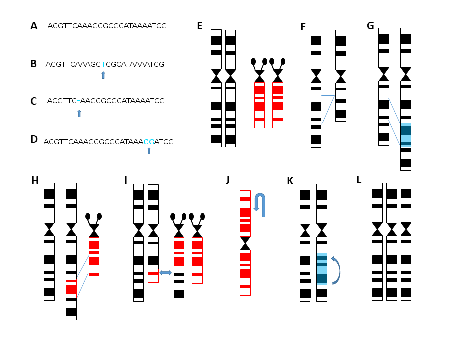
\includegraphics[width=1.0\linewidth]{img/Introduction_Fig1}
	\caption[Human genome variation types]{Human genome variation types: A) genomic base sequence, B) Single nucleotide variant, C) Indel: one base deletion, D) Indel: two base insertion, E) Two sets of chromosomes, F) CNV: Deletion, G) CNV: duplication, H) CNV: insertion, I) Reciprocal translocation, J) Robertsonian translocation, K) Inversion, L) Aneuploidy: trisomy}
	\label{fig:Introduction_Fig1}
\end{figure}



\section{Conventional techniques for variant detection} \label{intro_traditional}
Over the years many different techniques have been developed to detect and chart the DNA constitution. 
The earliest was karyotyping, the technique used by Tjio and Levan, in which metaphase spreads are made that enable analysis of chromosomes using a microscope \cite{Tjio_1956}. 
The development of chromosome staining techniques, such as Q,- C-, G- and R-banding, increased the resolution to a maximum of 5 Mb and enabled detection of smaller aberrations as well as more-specific determination of known variations \cite{Hamerton_1972,Liu_2015}. 
In situ hybridization techniques using radio- or fluorescent-labelled probes enabled detection of the presence and localization of specific parts of chromosomes \cite{Gall_1969,Bauman_1980,Levsky_2003}. 
It is particularly the latter, Fluorescence In Situ Hybridization (FISH), that paved the way for subchromosomal structural analysis, making it possible to detect microdeletions of several hundreds of kilobases (kb) \cite{Cui_2016}. 
Further developments of this technique, such as fiber-FISH, increased the resolution to 50 kb using mechanically stretched chromosomes \cite{Raap_1996}.
While these molecular techniques greatly advanced cytogenetics, analysis of solid tumors remained difficult because often no high-quality metaphases can be produced. 
Comparative Genomic Hybridization (CGH), an adaptation of FISH procedures, in which all patient DNA is fluorescently labelled and hybridized together with differently labelled reference DNA to high quality metaphases of a normal cell line enabled evaluation of aneuploidies, unbalanced translocations and CNVs \cite{Kallioniemi_1992}.
In other words, all types of variations resulting in loss or gain of chromosomal material could be detected genome-wide to a maximum resolution of 10 Mb for deletions and 2 Mb for amplifications, without the need of patient metaphase spreads \cite{James_1999b}. 
The same principle was used in array-CGH but, instead of metaphase spreads, a series of probes were used as the hybridization target, making it possible to detect CNVs smaller than 1 kb depending on the number and placing of the probes \cite{Pinkel_1998,Boone_2010}. 
Using knowledge gained by earlier sequencing projects, it became possible to target specific SNPs, enabling the array to be used not only for CNV detection, but also as a genotyping tool \cite{Wang_1998}. 
A targeted technique to further enhance the resolution for CNV detection is Multiplex-Ligation Probe Amplification (MLPA), in which several targeted stretches of DNA are amplified in one experiment, after which a relative comparison is done within a series of samples. 
Depending on the included targets, deletions or duplications of single exons can be detected \cite{Schouten_2002}.

Where cytogenetics and molecular cytogenetics focused on the detection of structural variations, including copy-neutral variations and aneuploidies (figure \ref{fig:Introduction_Fig1}E-L), molecular genetics focused on the detection of the nucleotide sequence, searching for SNVs, indels and repeat expansions (figure \ref{fig:Introduction_Fig1}A-D). 
Often, Sanger sequencing was the method of choice here. 
However, only a short stretch of DNA of a single sample can be analyzed in a single experiment using this technique. 

Variants are not always expected to be present in all cells from all tissues, as is the case with genetic mosaicism, including mitochondrial heteroplasmy, as well as in cancer. 
In karyotyping or FISH, a separate analysis is performed for each cell. 
By analyzing a large number of metaphases or nuclei, mosaicisms can be detected or excluded with high probability in the tissue studied \cite{Hook_1977,Sikkema_1997,Wolff_2007}. 
Several DNA-based methods are also able to assess the presence of low fractions of a certain type of DNA in a larger pool. 
Real-time quantitative PCR measures fluorescence after each PCR cycle, then, through comparison with samples having a known concentration, fractions of targeted DNA stretches can be calculated for a sample \cite{Heid_1996}. 
Quantitative fluorescent (QF-)PCR measures the DNA concentration after a fixed number of PCR cycles \cite{Eggeling_1993}. 
A more recent addition is digital droplet PCR (ddPCR), where DNA fragments are encapsulated in oil droplets. 
For each droplet it is determined if a specific DNA sequence is present or not. Because tens of thousands droplets can be assessed in a single experiment, this technique has a high sensitivity for low-abundance variations \cite{Hindson_2011}.

It is no coincidence that so many techniques have been developed for DNA analysis, as each technique has distinct strengths and weaknesses. 
In karyotyping at low resolution, chromosome specific analysis can be done for the whole genome of a single cell. 
FISH increases resolution, but only gives information about targeted regions, while array gives high resolution whole genome information, but can’t distinguish alleles and thus misses copy neutral structural variations. 
MLPA and Sanger sequencing have even higher resolution – the latter up to a single base pair – but, in a single experiment, are limited to analysis of a small part of the genome. 
Therefore, using these conventional techniques to find all types of variations present in a single sample requires many different experiments. 


\section[Next-generation sequencing]{Next-generation sequencing}\label{intro_ngs}
In the mid-2000s, massive parallel sequencing was developed. With the introduction of this method, there was an immediate 50,000 fold drop in sequencing costs, resulting in the label ‘next-generation sequencing’ (NGS) \cite{Goodwin_2016}. 
NGS can be used for DNA as well as RNA sequencing. 
While the term NGS might suggest a single technique, it is in fact an umbrella-term encompassing many different technologies that sequence many DNA or RNA fragments in parallel and infer a read of the nucleotide sequence of each fragment.
The first NGS platform available was developed by 454 Life Sciences using a pyrosequencing strategy \cite{Margulies_2005}. 
Solexa then introduced NGS using reversible dye terminator chemistry \cite{Bentley_2008} and Ion Torrent a non-optical system based on pH changes on nucleotide incorporation \cite{Rothberg_2011}. 
With these technologies being acquired by Roche, Illumina and Life Technologies, three strong contenders entered the short-read sequencing market. Other platforms focus on sequencing long single DNA molecules, such as Pacific Biosystems \cite{Eid_2009} and Oxford NanoPore \cite{Clarke_2009}, making use of real-time measurements of fluorescent signals and changes in current, respectively. 
Other contenders have since entered and left the NGS market, all using different chemistry and measurement tools. Because of this, technical bias is different from one technique to the other, although some genomic regions still remain a challenge for all platforms. 

Although the exact methods used differ between different NGS techniques, their general approach is similar, as shown in figure \ref{fig:Introduction_Fig2}, although the strong and weak points vary between the platforms. 
For NGS DNA analysis, various input materials can be used. 
Some contain fragmented DNA, such as blood plasma or formalin-fixed paraffin-embedded (FFPE) material (figure \ref{fig:Introduction_Fig2}A), while others contain high quality DNA, for example white blood cells, bone marrow or cultured cells (figure \ref{fig:Introduction_Fig2}B). 
The first step in all DNA NGS procedures is to isolate DNA from the material. 
In the materials where the DNA is already fragmented, short DNA fragments are isolated (figure \ref{fig:Introduction_Fig2}C).

\begin{figure}
	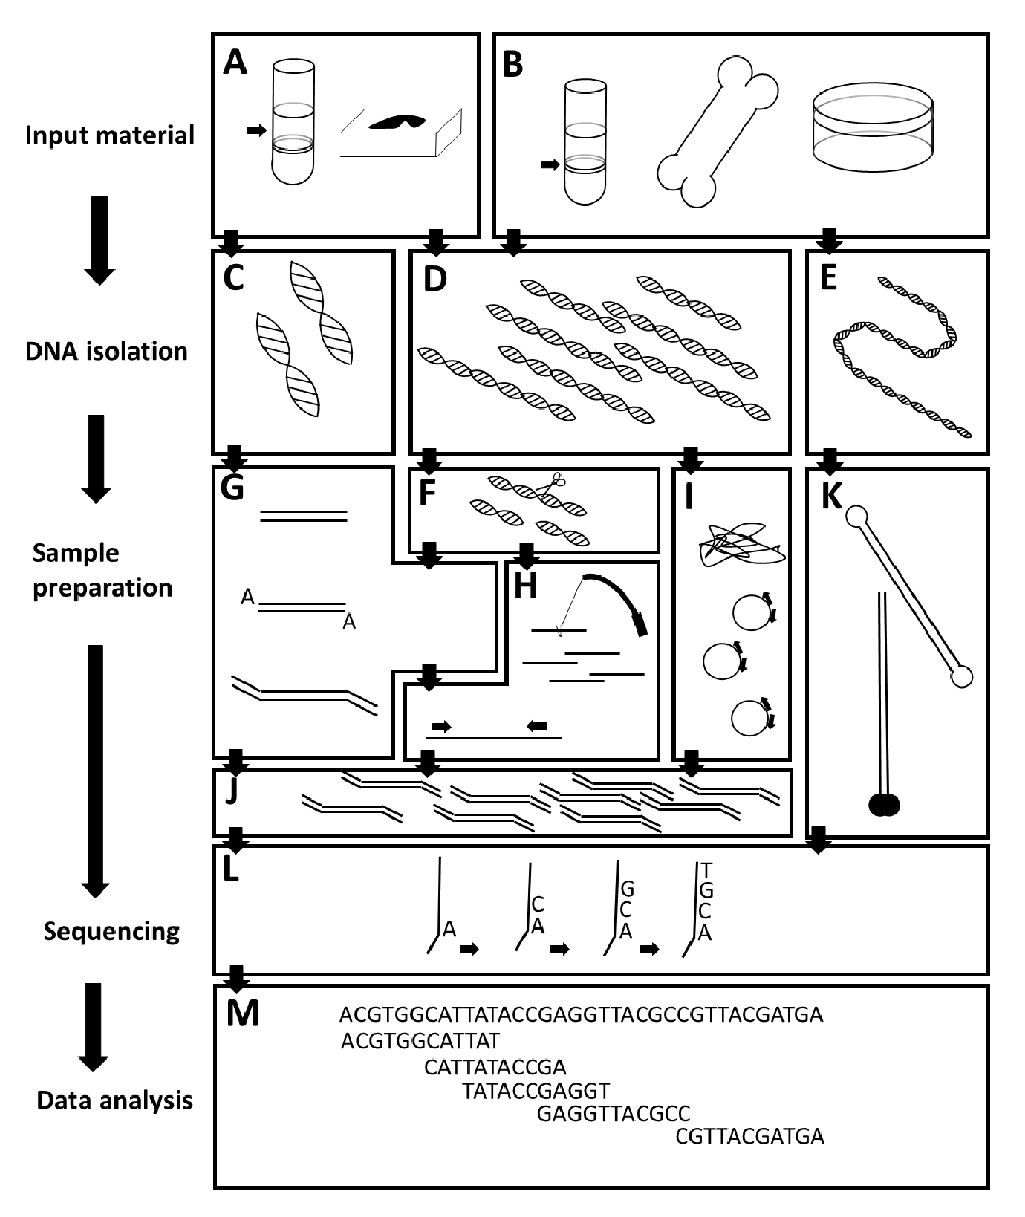
\includegraphics[width=1.0\linewidth]{img/Introduction_Fig2}
	\caption[DNA Next-generation sequencing workflows]{DNA Next-generation sequencing workflows. A) Sources of fragmented DNA, such as blood plasma or FFPE material, B) sources of high quality DNA, such as white blood cells, bone marrow cells or cultured cells, C) isolated fragmented DNA, D) isolated high-quality DNA, E) isolated long fragments of DNA, F) DNA fragmentation, G) sample preparation (end-repair, dA-tailing and adapter ligation), H) enrichment via capturing or amplicon sequencing), I) alternative sample preparation, such as Targeted Locus Amplification or ATAC-seq, J) PCR, K) long-read sequencing sample preparation, L) sequencing of the DNA, M) data analysis to transform sequenced DNA into sequence reads and subsequently into sample-specific genomic sequences.}
	\label{fig:Introduction_Fig2}
\end{figure}

Source materials containing higher quality DNA can give rise to longer DNA-fragments (figure \ref{fig:Introduction_Fig2}D) or even very long DNA fragments, if DNA breakage is prevented during isolation (figure \ref{fig:Introduction_Fig2}E). 
The short-read sequencing methods work best when using relatively short DNA fragments. 
For these techniques, DNA needs to be fragmented if the input fragments are too long (figure \ref{fig:Introduction_Fig2}F). 
The most basic short-read strategy is whole genome sequencing (WGS). 
Sample preparation consists of adding so-called ‘adapters’ to DNA-fragments, thus making the fragments suitable for sequencing (figure \ref{fig:Introduction_Fig2}G). 
If only a part of the genome needs to be sequenced, the DNA can be enriched for the sequences of interest (figure \ref{fig:Introduction_Fig2}H). 
Various methods can be used to reach this goal, such as DNA capturing, in which short RNA or DNA sequences complementary to the region of interest called ‘baits’ are used to fish out specific parts of the genome.
A second method is amplicon sequencing. Here, similar to Sanger sequencing, two primers are used that bind to their complementary sequence and copy the genomic sequence in between the primers. Such enrichment techniques are used in, for instance, whole exome sequencing (WES) and gene panels that target specific genes of interest. 
In addition to these ‘standard’ sample preparation methods, alternative sample preparations can be performed that have a different perspective on the genome (figure \ref{fig:Introduction_Fig2}I), for instance using proximity ligation \cite{Spielmann_2018}, targeted locus amplification \cite{de_Vree_2014}, or chromatin-immunoprecipitation or by enzymatic digestion \cite{Jiang_2018}.
 
The final step in the sample preparation is PCR amplification to produce sufficient fragments of the DNA of interest to be sequenced (figure \ref{fig:Introduction_Fig2}J). 
Alternatively, long-read sample preparation methods can be used (figure \ref{fig:Introduction_Fig2}K). 
The bases of the DNA fragments are subsequently read by the sequencer (figure \ref{fig:Introduction_Fig2}L). 
Data analysis is then carried to determine the nucleotide sequence of the DNA fragments, and the genomic sequence of the sample can be inferred through further processing, for instance through alignment of sequenced reads to a reference genome (figure \ref{fig:Introduction_Fig2}M). 
Once the genomic sequence is inferred as far as possible, the presence or absence of variants can be de determined and interpreted in the context of a scientific or diagnostic question. 
An important step in variant calling and interpretation is to distinguish true positive and negative results from false ones. 
Knowing where variants can be missed, or where artefacts are more likely to occur, can be important for making a correct interpretation. 
Moreover, if the cause of artefacts is known, analysis procedures can be adapted to counteract sources of bias and create a more optimal balance between sensitivity and specificity. 


\section[Technical bias and error rates]{Technical bias and error rates}\label{intro_bias}
Where conventional techniques have proven their worth in genetic diagnostics, NGS procedures and analysis still need to be optimized, and refining the methods to improve their sensitivity and specificity remains a challenge. 
The aim of the different NGS techniques is to measure the exact nucleotide sequences of the DNA fragments. 
However, technical bias and sequencing errors create noise, resulting in some of the nucleotides in a sequence read being called incorrectly. 
This error rate is much higher for long-read technologies than for short-read sequencing. Depending on the chemistry and platform used, error rates range from 0.1\% to 15\% \cite{Goodwin_2016}. 
These error rates are presented as base quality scores and, when several reads are combined to infer a genotype, as a genotype quality score \cite{Nielsen_2011}. 
However, it has been shown that discordance rates between short-read samples that have been analyzed twice are higher than would be expected using the genotype quality scores \cite{Wall_2014,Schirmer_2015}, which suggests that error rates are higher than the sequence data lead us to believe. 
Whereas some of the sequencing errors are random, each type of sequencer, as well as each experimental design, has its own systematic biases that occur at specific sequence patterns, inverted repeats or homopolymers \cite{Nakamura_2011,Schirmer_2015}. 
Because some of the errors are made during PCR amplification, base quality scores are not always sufficient to determine the chance that a specific base is called correctly for a sequenced DNA fragment.
This is especially important when the aberration of interest is expected to occur in only a subset of the analyzed DNA fragments, as is the case for germline and somatic mosaic variants and for non-invasive prenatal testing (NIPT), where fetal DNA is analyzed in the presence of maternal DNA, because fewer sequence reads will be present to support a genotype call. 
An important contributor to the creation of bias during PCR is the GC percentage in the DNA fragment. If a high (\textgreater65\%) or low (\textless12\%) percentage of guanine or cytosine bases are present, the DNA fragments are barely amplified during PCR, with the amplification efficiency gradually increasing with GC percentages closer to 50\% \cite{Aird_2011}. 
With each PCR cycle needed in the experiment, the GC bias will grow, although this bias can also occur during PCR-steps that are part of the sequencing procedure itself \cite{Roeh_2017}. 
The severity of this bias can differ between samples and experiments. 
An extra effect of using many PCR cycles in sample preparation is that the number of reads originating from the same DNA fragment, called duplicate reads, will grow. 
This can lead to a risk of overestimating the effective coverage and sensitivity as well as the chance of amplifying errors occurring during extension in early PCR cycles, thus reducing specificity.  

For WGS, fewer PCR cycles are usually needed in the sample preparation, leading to a relatively even coverage between different genomic regions. 
However, targeted techniques such as WES and targeted NGS (tNGS) that rely on selective amplification of genomic regions of interest require PCR during sample preparation. 
In general, the rule applies that the lower the amount of input material or the smaller the targeted region, the more PCR cycles are needed, up to more than 30 cycles for some procedures. 
At 30 PCR cycles, over a billion copies of the same original DNA fragment are generated. 
In contrast, after 10 PCR cycles, just over one thousand copies are present. 
When randomly sheared DNA fragments are amplified and sequenced, duplicate reads can, to a certain extent, be identified based on the fact that they have an (almost) identical sequence. 
However, in amplicon-based sequencing, which uses primers to amplify a region of interest, it is expected that different original DNA fragments give rise to reads with the same sequence. 
This makes it more difficult to distinguish those reads from each other, unless separate molecular identifiers are used. 

But, even when all technical bias is corrected for, not all parts of the genome are accessible, especially in short-read sequencing. 
Many parts of the genome are not unique, for instance genes that have pseudogenes \cite{Mandelker_2016}. 
When a DNA-fragment originating from such a region is sequenced, there is no way to determine from the sequenced read itself if it is informative for the region of interest or for the other region that has the same sequence. 


\section{DNA variant detection in genome diagnostics} \label{intro_diagnostics}
In current genome diagnostics many of the DNA variant detection methods described in sections 1.3 and 1.4 are used. 
The types of variations that are searched for, as shown in figure 1.1, are different for different diagnostic questions. 
Moreover, the variants being examined can be present in only some of the cells – and therefore only part of the DNA analyzed – as discussed earlier. 
In the paragraphs below I discuss three important types of variants that need specific analysis and interpretation approaches: germline variants, somatic variants and variants found in prenatal testing. 

\subsection{Germline variants}
Germline variants are present at the formation of the zygote and, in principle, are present in all cells, including the germline \cite{Griffiths_2000}. 
For genetic analysis, white blood cells or fibroblasts provide a source of high-quality DNA. 
Germline variants can be transmitted from parent to child and can therefore result in multiple affected relatives within a family. 
Depending on the nature of the variants, a disease phenotype may develop during childhood, or adulthood, or even not at all. For Mendelian diseases the inheritance pattern for variants in autosomal chromosomes (i.e. chromosomes 1-22) can be autosomal dominant (AD) or autosomal recessive (AR). 
In AD inheritance, a variant in only one of the alleles can result in the disease phenotype. 
In AR inheritance, both parents transmit a pathogenic variant. 
Variants present in sex-chromosomes or mitochondria have different inheritance patterns. 
Because men carry one copy of each sex chromosome, a sex-chromosome-related recessive trait will result in a phenotype when a single copy of the causal variant is present. 
Mitochondria are always transmitted from mother to child, leading to phenotypes caused by mitochondrial variants only being inherited through the maternal line. 

One example of an AD hereditary disease is Lynch syndrome, one of the most common cancer predisposition syndromes. 
In Lynch syndrome, SNVs, indels, intragenic deletions or duplications cause a deficiency in the mismatch repair system that significantly increases the risk of developing cancer compared to the general population, although, as in other cancer-predisposing syndromes, not all carriers of pathogenic variants develop cancer \cite{Tutlewska_2013,Talseth_Palmer_2016}. 
It is estimated that around 1 in 300 people carry a pathogenic variant in one of the genes associated with Lynch syndrome \cite{Cancernet_2005}. 
One of the most common AR disorders is cystic fibrosis, which leads to dysfunctional chloride channels that cause thickened mucus and affects around 1 in 3500 individuals in Europe \cite{Yu_2018,Scotet_2012}. 
Children with cystic fibrosis often inherit a non-functional allele of the \textsl{CFTR} gene from both of their parents, who themselves don’t present with the disease phenotype because they have a functional copy of the gene. 
An example of a common recessive X-linked trait is red-green color-blindness, which affects 1 in 12 males and 1 in 200 females in populations with Northern-European ancestry \cite{Geneticshomereference_2019}. 
The prevalence of mitochondrial diseases is highly dependent on the population and is associated with, among other conditions, neurological diseases and ataxia \cite{Chinnery_2018}.

It is also possible that variants appear \textsl{de novo} during de formation of the gametes. 
\textsl{De novo} means that a variant is found in an individual even though neither of the parents carry this variant. 
Such a variant can arise through mistakes in copying DNA for SNVs and indels, through errors in crossing over for SVs, or through non-disjunction for aneuploidies. 
Examples of syndromes caused by SVs are Down syndrome (trisomy 21), Klinefelter syndrome (XXY), Turner syndrome (X0), Di-George syndrome (del 22q11) and the 1q21.1 microduplication syndrome.


\subsection {Somatic variants}
When a DNA variant is not present in the zygote but rather originates from a later cell division, it is called a somatic variant. 
If such a variant originates during embryonic development, it will be present in many cells; if it occurs later in life, it may be present in a small number of cells \cite{Frank_2014}. 
Some of the syndromes mentioned in the previous paragraph, Down syndrome and Turner syndrome for instance, can have their origin not only in germ cells, but also be the result of somatic mosaics. 
Mosaics may not lead to a clinical abnormal phenotype, depending on the distribution of the somatic variants over cells and tissues. 
Low level mosaics in parents that include their germ cells may be difficult to distinguish from \textsl{de novo} cases discussed in the previous section. 
Mosaics may also arise through a germline variation with a rescued cell-line in which the variation is eliminated \cite{Devlin_2004,Hook_2014}. 

Some disorders such as segmental neurofibromatosis \cite{Sobjanek_2014} or McCune-Albright syndrome \cite{Dumitrescu_2008}, in which parts of the body are affected while other parts are unaffected, are caused by mosaics. 
In cancer, somatic variants are the main cause of tumorigenesis. 
A tumor can develop when a gene variant causes uncontrolled cell division, as is the case with the Philadelphia chromosome \cite{Kang_2016}, or fails to lead the cell into appropriate cell-death, as is the case with variations affecting the \textsl{MYC} gene \cite{Dominguez_Sola_2014}. 
A cell that develops such a variant can then grow into a clonal population, which can later on develop into further subclones, together constituting the tumor cells \cite{Nowell_1976,Naugler_2010,McGranahan_2017}. 
In advanced disease stages, some variants can be present in a high percentage of cells. 
However, in earlier stages, after treatment or when a new variant has arisen in a subclone, it can be the case that only a small percentage of the cells analyzed carry the variant. 
In addition, tumor samples sent in for analysis typically contain both tumor cells and normal cells (e.g. lymphocytes or stromal cells), which adds to the mosaic nature of gene variants in these samples.

Somatic variants in tumor or hematological cells can consist of all the variant types described in section 1.2. 
However, while large structural variants, including aneuploidies, are rare events when looking at germline variants, they are more prevalent in cancer cells, where complex aberrant karyotypes are also seen. 
The main challenge for somatic variant detection in tumors is the possible presence of a wide variety of DNA variants and, sometimes balanced, chromosomal aberrations in a low percentage of the cells or DNA to be analyzed. 
In addition, the material containing the variations, such as bone marrow or tumor material, is harder to come by and often of lower quality than that used for germline variation detection.


\subsection{Prenatal testing}
Genetic variants can also be detected prenatally. 
Conventionally, such tests are offered to pregnant women at an elevated risk of carrying a child with a chromosomal abnormalities, most notably Down syndrome, Patau syndrome (trisomy 13) and Edwards syndrome (trisomy 18), and for hereditary disease-causing-gene variants previously identified in one or both of the parents. 
Conventional invasive prenatal tests are performed using cells from the fetus or from extra-fetal tissue that shares genetic origin with the fetus: amniotic fluid cells (fetal and extra-fetal origin) or chorionic villi cells (extra-fetal, placental). 
The main problem with the frequently used types of invasive procedures – amniocentesis and chorionic villi biopsy – is a risk of a procedure-related miscarriage of 0.3\% and 0.5\%, respectively \cite{Beulen_2017}. 
Fortunately, the mother’s blood can also be used as a source of short fragments of extra-fetal DNA \cite{Lo_1997}. 
This so-called cell-free fetal DNA (cffDNA) circulates through the blood stream of a pregnant woman, next to a greater fraction cell-free DNA (cfDNA) originating from her own cells. 
On average only around 12\% of the cfDNA is cffDNA, though it can be much lower \cite{Ashoor_2012a}. 
The cfDNA, including the cffDNA, can be isolated from blood plasma to enable non-invasive prenatal testing (NIPT). 
Because no invasive procedures are needed in NIPT, there is no risk of inducing a miscarriage. For this reason, NIPT has quickly become a mainstream genetic test. 
In the Netherlands NIPT has been offered to women with a high risk of carrying a child with a trisomy 13, 18 or 21 since 2014 and to all pregnant women since 2017 \cite{meeroverNIPT_2018}. 
However, because a mosaic of cffDNA and maternal cfDNA is present, similar technical challenges have to be overcome to those faced in somatic variant testing.	 

\section {Aims of this thesis} \label{intro_aims}
As we have seen throughout the introduction, many different DNA variants can be present in a single sample. 
However, technical bias, size of the variation, copy-neutrality of variations, mixed cell-populations or DNA samples and the biological origin of analyzed DNA fragments can all create noise in the analysis process. 
The task of the clinical genetics laboratory is to look through this noise to detect and interpret the presence or absence of relevant variants. 
When using conventional techniques, many independent tests are needed to overcome different types of noise or to change resolution, sensitivity, number of variants analyzed and the ability to detect balanced variants or not. NGS has the potential to replace all these tests. 
However, not all types of variants are easy to detect. 
By using efficient sample preparation and analysis algorithms that can distinguish artefacts from variants, NGS is able to challenge conventional techniques and may become the method of choice for all diagnostic questions related to the detection of DNA variants.

The studies in this thesis aim to improve NGS DNA analysis for detection of germline SNVs, indels and CNVs, somatic translocations and trisomy detection through NIPT, as well as interpretation of analysis outcomes. 
In this thesis, I introduce new tools, methods and algorithms for NGS DNA analysis and interpretation and, in some cases, use them in a practical application (figure \ref{fig:Introduction_Fig3}). 

\begin{figure}
	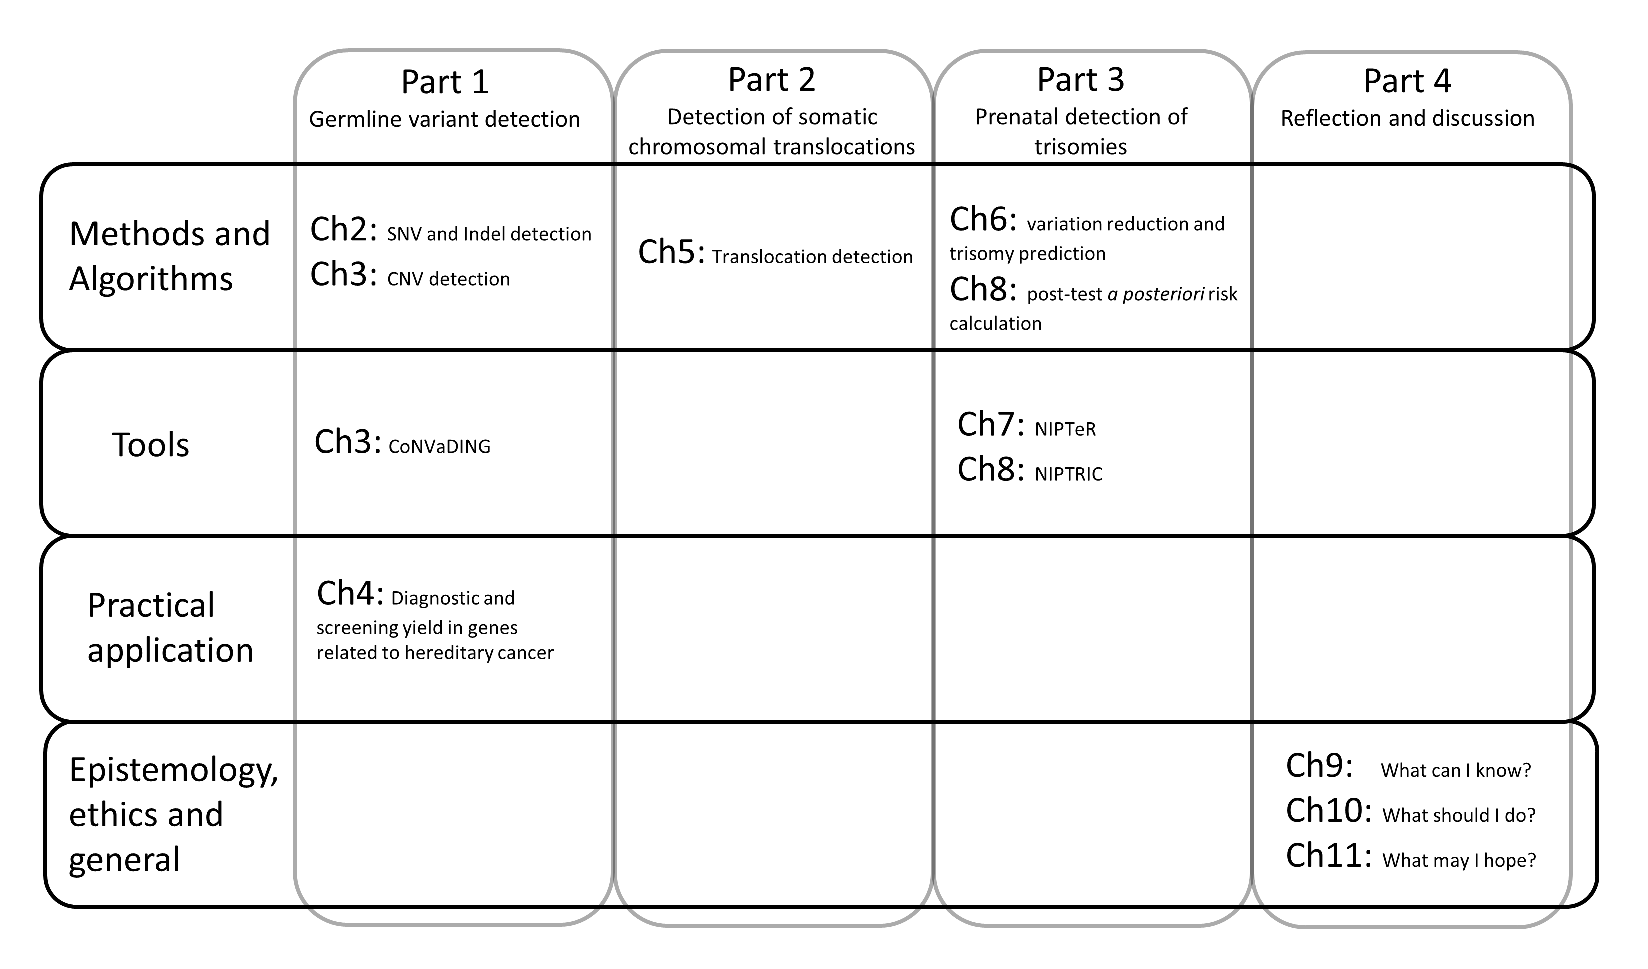
\includegraphics[width=1.0\linewidth]{img/Introduction_Fig3}
	\caption[Overview of the topics addressed in the thesis chapters ]{Overview of the topics addressed in the thesis chapters.}
	\label{fig:Introduction_Fig3}
\end{figure}

\subsection[Germline variant detection]{Part 1:  Germline variant detection \newline (chapters 2, 3 and 4)}\label{Part 1}
The most prevalent germline variants – SNVs, indels and small CNVs – were conventionally analyzed mainly using Sanger sequencing for SNV and indel detection and MLPA to detect CNVs. 
However, only a short stretch of DNA can be analyzed in each measurement using these techniques, limiting the number of genes that can by analyzed in a single experiment. 
In chapter 2 we set out to implement tNGS as a stand-alone diagnostic test to enable analysis of a large set of genes in a single test and replace Sanger sequencing in clinical diagnostics. For this we developed, validated and established quality criteria for a tNGS genepanel to detect SNVs and indels with high sensitivity and specificity in 48 genes involved in cardiomyopathies, ultimately demonstrating that tNGS is a technique suitable for diagnostic use. 
In chapter 3 we further expand the application of tNGS and enable simultaneous detection of CNVs up to the single exon level, next to SNVs and indels. 
Because it is likely in tNGS that CNV breakpoints are located outside targeted regions, CNVs can only be inferred through analysis of read depth. 
However, laboratory-induced variability of read depth is larger than biological variability. 
To look through the experimental noise and detect (single-exon) CNV in tNGS data, we introduce new algorithms with strict quality control that we implement in the open-source tool CoNVaDING (\textbf{\underline{Co}}py \textbf{\underline{N}}umber \textbf{\underline{Va}}riation \textbf{\underline{D}}etection \textbf{\underline{I}}n \textbf{\underline{N}}ext-generation sequencing \textbf{\underline{G}}ene panels). 
In chapter 4 we set out to use the tools and methods developed in the previous chapters in the context of hereditary cancer, for which we have analyzed 85 genes in 2,090 patients and 1,326 individuals from the general Dutch population. 
The first goal here was to determine the diagnostic yield, focusing on genes with a relation to the cancer type warranting referral. 
The second goal was to determine the findings if, in addition to these genes, we search for pathogenic or likely pathogenic variants in genes without such a relation (secondary findings), and how often variants leading to a cancer predisposition occur in the general Dutch population. 

\subsection[Detection of somatic chromosomal translocations]{Part 2: Detection of somatic chromosomal \newline translocations (chapter 5)}\label{Part2}
The second part of this thesis consists of a single chapter that focuses on somatic translocation detection. 
In current hematological malignancy diagnostics SVs, including translocations, are detected using various conventional techniques. 
Using karyotyping, large rearrangements are detected on a single-cell basis. 
However, this technique is unable to detect some so-called cryptic translocations. 
FISH and RT-PCR are needed to detect those, but these techniques can only target one SV or fusion-gene at a time. 
In chapter 5 we aim to develop an NGS-based technique to target 18 genes and detect translocations involving one of those genes commonly involved in acute leukemia, regardless of their translocation partner, to be suitable for use as a first-line screening tool in diagnostics. 
For this we make use of Targeted Locus Amplification (TLA) \cite{de_Vree_2014} to create a multiplex TLA acute leukemia gene panel. In addition to the genes themselves, our panel captures DNA physically close to the targeted genes, which enables the capture and detection of chromosomal translocation partners even if they are not in the targeted panel. 
We develop analysis and interpretation strategies and demonstrate for several targeted genes that the panel detects translocations involving those genes at 10\% aberrant cells. 
We conclude that multiplex TLA is a promising technique that it needs further optimization before it can replace conventional methods.

\subsection[Prenatal detection of trisomies]{Part 3: Prenatal detection of trisomies \newline (chapters 6, 7 and 8)}\label{Part3}
Part three of this thesis is dedicated to NIPT. Where conventional methods for prenatal trisomy detection, such as karyotyping, FISH, QF-PCR or array, rely on invasive procedures, NIPT can be performed using ultralow-coverage NGS data. Using a basic sample preparation with as few PCR cycles as possible, the short cfDNA fragments are made available for sequencing. 
Several algorithms are described in the literature to analyze such ultralow-coverage NGS data to predict the presence of a trisomy \cite{Chiu_2008,Fan_2010,Sehnert_2011}. 
These strategies rely on the comparison of the sample of interest to a group of non-trisomy control samples to determine if significantly more sequence reads are present that originate from DNA fragments of the potential trisomic chromosome. 
Because cffDNA is mixed with maternal DNA, a trisomy will only cause a small increase in the fraction of reads of the chromosome involved. 
Therefore it is important to make the variability in chromosomal fractions as small as possible between samples. 
In chapter 6 we introduce novel algorithms to analyze ultralow-coverage NGS data and obtain a higher sensitivity for trisomy detection than found using earlier described calculations. 
In addition, we create a quality metric that can be used to detect if the available reference samples are suitable for comparison with the sample analyzed. 
In chapter 7 we describe \textsl{NIPTeR}, an open-source R package that makes the algorithms developed in chapter 6 available along with the algorithms described in the literature for analysis of NIPT data. 

Two women receiving a similar test result from NIPT do not necessarily have a similar risk of carrying a child with a trisomy. 
In chapter 8 we focus on the clinical interpretation of the NIPT result, taking into account not only biological and technical characteristics of the test, but also the population to which the woman being tested belongs. 
Including these pre-test conditions in the interpretation might result in different risk profiles for women from different risk-groups who have the same raw test result. 
We created algorithms to calculate such a personalized post-test risk for a specific fetal trisomy and made these available in NIPTRIC, an online calculator. 

\subsection[Reflection and discussion]{Part 4: Reflection and discussion \newline (Chapters 9, 10 and 11)}\label{Part4}
Inspired by the three questions posed by Immanuel Kant in his \textsl{Kritik der reinen Vernunft} published in 1781/1787: “what can I know?”, “what should I do?” and “what may I hope?” \cite{Kant_1781a}[p.728], in part four of this thesis I reflect on and discuss the methods, tools and algorithms described in this thesis. 
In chapter 9 I look back on the chapters from an epistemological point of view. 
In genetic diagnostics we infer the genetic or genomic constitution of a person through a measurement outcome. 
I elaborate on the concept of noise that I define as ‘everything that, from a certain perspective, blocks the path between reality and measurement outcome’. 
Throughout this thesis we are battling four types of such noise: biological noise, laboratory-induced noise, sequencing noise and data analysis noise. 
The variants of interest are hidden behind this noise, but through innovative perspectives we are better able to look through the noise and correctly interpret measurement outcomes. 

In chapter 10 I make an ethical reflection on the technologies introduced in this thesis. I use the theories of Peter-Paul Verbeek who states that artefacts are morally charged and mediate human action \cite{Verbeek_2011}[p.21]. 
I try to uncover intended and unintended moral consequences of the availability of the methods, tools and algorithms presented in this thesis. 

In chapter 11 I address the last question of Kant: ‘what may I hope?’ and put the work presented in this thesis in broader perspective in the general discussion and give future perspectives on developments in NGS DNA analysis.


\chapter*{\fontsize{36}{50}\selectfont Part 1}
\chaptermark{Part 1}
\label{chap:part1}

\addcontentsline{toc}{chapter}{Part 1: Germline variant detection}
\chapter[targeted NGS can replace Sanger sequencing in clinical diagnostics]{Targeted Next-Generation Sequencing can Replace Sanger Sequencing in Clinical Diagnostics}
\chaptermark{targeted NGS in clinical diagnostics}
\label{chap:SNP and Indel detection}

{ \Large \leftwatermark{
		\put(-67,-66.5){ 1 }
		\put(-76.5,-100){
\includegraphics[scale=0.8]{img/thumbindex.eps}} \put(-67,-91.5){ {\color{white} 2 }}
		\put(-67,-116.5){ 3 }
		\put(-67,-141.5){ 4 }
		\put(-67,-166.5){ 5 }
		\put(-67,-191.5){ 6 }
		\put(-67,-216.5){ 7 }
		\put(-67,-241.5){ 8 }
		\put(-67,-266.5){ 9 }
		\put(-67,-291.5){ 10 }
		\put(-67,-316.5){ 11 }
	} \rightwatermark{
		\put(350.5,-66.5){ 1 }
		\put(346.5,-100){
\includegraphics[scale=0.8]{img/thumbindex.eps}} \put(350.5,-91.5){ {\color{white} 2 }}
		\put(350.5,-116.5){ 3 }
		\put(350.5,-141.5){ 4 }
		\put(350.5,-166.5){ 5 }
		\put(350.5,-191.5){ 6 }
		\put(350.5,-216.5){ 7 }
		\put(350.5,-241.5){ 8 }
		\put(350.5,-266.5){ 9 }
		\put(350.5,-291.5){ 10 }
		\put(350.5,-316.5){ 11 }
}}

\hfill \underline{Human Mutation} 2013;34(7):1035-42.

\hfill DOI: \href{https://doi.org/10.1002/humu.22332}{10.1002/humu.22332}

\hfill PubMed ID: \href{https://www.ncbi.nlm.nih.gov/pubmed/23568810}{23568810}

\newpage

\noindent
L.F. Johansson\textsuperscript{1,2,*}, F. van Dijk\textsuperscript{1,2,*}, E.N. de Boer\textsuperscript{1}, K.K. van Dijk-Bos\textsuperscript{1}, L.G. Boven\textsuperscript{1}, M.P. van den Berg\textsuperscript{2}, K.Y. van Spaendonck-Zwarts\textsuperscript{1}, J. Peter van Tintelen\textsuperscript{1}, R.H. Sijmons\textsuperscript{1}, J.D. Jongbloed\textsuperscript{1},  R.J. Sinke\textsuperscript{1} \\

\noindent
1. University of Groningen, University Medical Center Groningen, Department of Genetics, Groningen, The Netherlands\\
2. University of Groningen, University Medical Center Groningen, Department of Cardiology, Groningen, The Netherlands\\


\noindent
Received 2013 Jan 9; Accepted revised manuscript 2013 Apr 2; Published online 2013 Apr 4.
\\~\\
* Contributed equally

\section*{Abstract}\label{abstract}
Mutation detection through exome sequencing allows simultaneous analysis of all coding sequences of genes. 
However, it cannot yet replace Sanger sequencing (SS) in diagnostics because of incomplete representation and coverage of exons leading tomissing clinically relevant mutations. 
Targeted next-generation sequencing (NGS), in which a selected fraction of genes is sequenced, may circumvent these shortcomings. 
We aimed to determine whether the sensitivity and specificity of targeted NGS is equal to those of SS. 
We constructed a targeted enrichment kit that includes 48 genes associated with hereditary cardiomyopathies. 
In total, 84 individuals with cardiomyopathies were sequenced using 151 bp paired-end reads on an Illumina MiSeq sequencer. 
The reproducibility was tested by repeating the entire procedure for five patients. 
The coverage of $\geq$30 reads per nucleotide, our major quality criterion, was 99\% and in total {\textapprox}21,000 variants were identified. 
Confirmation with SS was performed for 168 variants (155 substitutions, 13 indels). 
All were confirmed, including a deletion of 18 bp and an insertion of 6 bp. 
The reproducibility was nearly 100\%. 
We demonstrate that targeted NGS of a disease-specific subset of genes is equal to the quality of SS and it can therefore be reliably implemented as a stand-alone diagnostic test.

\section{Introduction}\label{introduction}
Next-generation sequencing (NGS) techniques have significantly increased the possibilities of genome analysis. 
If we focus on diagnostic applications, mutation analysis through exome sequencing (ES) allows for the simultaneous analysis of all coding sequences of genes. 
One of the first clinical applications of ES was the detection of disease-associated mutations in rare Mendelian diseases, such as Miller syndrome \cite{Ng_2009}, Sensenbrenner syndrome \cite{Gilissen_2010}, and Schinzel–Giedion syndrome \cite{Hoischen_2010}. 
The advantage of ES is that it does not require a priori knowledge of gene(s) responsible for a disorder using it as a genetic discovery panel. 
In diagnostics, ES is already used to screen for de novo pathogenic mutations in intellectual disability \cite{de_Ligt_2012} explained by more than 1,000 different genes. 
In addition, ES can be used more targeted by analyzing only a panel of genes that may be involved in a particular disease. 
However, in routine diagnostics, detecting mutations via conventional Sanger sequencing (SS) is still the standard, despite the practical difficulties of keeping up with the ever-increasing numbers of test requests and of disease-associated genes. 
For instance, hereditary cardiomyopathies can be explained by 40-60 different genes \cite{Jongbloed_2011,Norton_2012} and effective analysis of all these genes by SS in a diagnostic setting is not feasible. 
In practice, it is limited to no more than 10 genes. 
In contrast, ES would allow the simultaneous analysis of all coding genes through enrichment for these coding regions before sequencing. 
However, in its current state, ES cannot be used as a reliable substitute for SS in diagnostics. 
A major shortcoming is incomplete representation and coverage of exons, leading to clinically relevant mutations being missed \cite{Gilissen_2010,Sulonen_2011}. 
Here, amore dedicated targeted enrichment appears to be the method of choice, not only because it allows focusing on the genes relevant for a particular disorder, but also because its highly effective enrichment provides a superior quality of representation and coverage. 
In addition, focusing on only the genes relevant for a particular disorder minimizes the problems associated with unsolicited findings. 
Targeted NGS is faster and cheaper than ES, especially for the analysis of certain distinct disease phenotypes. 
Various enrichment methods have been developed in the last few years, such as solid phase-based microarrays, micro-droplet-based PCR (Rain Dance Technologies, Lexington, MA), amplicon-based or solution phase-based methods such as Sure Select Targeted enrichment and Illumina TruSeq Customenrichment. 
Different types of platformshave also been developed for high-throughput sequencing. 
Recently, even bench-top instruments have become available, such as Ion Torrent PGM (Life Technologies Ltd, Paisley, UK), 454 GS Roche Junior (Roche Applied Science, Indianapolis, IN), and the Illumina MiSeq (Illumina, SanDiego,CA) \cite{Loman_2012}. 
These are the size of a modern laser printer and offer modest set-up and running costs; they are particularly suited to small projects and allow a fast throughput. 
The aim of our study was to validate targeted NGS for application in clinical diagnostics and to assess its sensitivity and specificity relative to SS. 
We therefore developed a SureSelect targeted enrichment kit (Agilent Technologies, Inc., Santa Clara, CA) for diagnostic testing of patients with hereditary cardiomyopathies. 
Hereditary cardiomyopathies are highly heterogeneous disorders, and include dilated (DCM), hypertrophic (HCM), and arrhythmogenic right ventricular cardiomyopathies (ARVC), which are leading causes of heart failure and sudden death. 
Approximately 30\%–50\% of DCM cases are familial, but with significant genetic and phenotypic heterogeneity \cite{Posafalvi_2012}. 
Particularly for DCM, for which more than 50 cardiomyopathy-related genes have been identified, targeted resequencing would be a much better diagnostic platform than SS. 
The use of a MiSeq bench-top machine would also enable short turn-around times in the laboratory. 
We compared the outcome of our targeted NGS experiments with results from SS, and discuss our findings in the light of validation, clinical laboratory implementation, and quality assessment in general.

\section{Material and Methods}

\subsection{Design of the Study}
Our study was divided into two parts: a validation phase and an application phase.
(1) Validation phase in which:
\begin{itemize}
	\item sequencing quality of the targeted NGS kit was measured in terms of representation and coverage;
	\item sequencing reliability was measured in terms of sensitivity compared with SS results for at least six out of 14 different cardiomyopathy-related genes.
\end{itemize}
(2) Application phase in which:
\begin{itemize}
	\item novel variants identified by our targeted NGS approach were confirmed by SS to assess the specificity;
	\item tests for reproducibility were performed. We set the following thresholds for accepting targeted NGS to replace SS in a diagnostic setting:
	\item Sequencing quality: coverage of at least×30 for each nucleotide, based on a normal binomial contribution, a minimum number of four reads for a call, a 20\% allele frequency resulting in a sensitivity of 99.96\% for a heterozygote.
	\item Sequence reliability in validation and application phase: 100\% sensitivity for at least 75 variants, including substitutions and indels. The specificity should be at least 98\%, that is, amaximum of 2\% false-positive variants.
	\item Reproducibility: 98\%, so that a maximum of 2\% difference in the variants within one sample was allowed when repeating the entire procedure. 
\end{itemize}

\subsection{Patients/Samples}
For the validation phase, we selected DNA samples of 24 patients diagnosed with dilated or arrhythmogenic cardiomyopathies. 
These patients had previously been analyzed by SS for up to six out of 14 disease genes (\textsl{DES}, \textsl{DSC2}, \textsl{DSG2}, \textsl{LMNA}, \textsl{MYBPC3}, \textsl{MYH7}, \textsl{PKP2}, \textsl{PLN}, \textsl{RBM20}, \textsl{SCN5A}, \textsl{TMEM43}, \textsl{TNNC1}, \textsl{TNNT2}, and \textsl{TNNI3}). 
Here, SS resulted in the identification of a disease-associated mutation in seven out of the 24 patients and a total of 90 variants. 
Subsequently, for the application phase, we selected a further 60 DNA samples of unrelated cardiomyopathy patients, for whom no causative mutation had been found by routine diagnostic testing by SS. 
All samples (n = 84) were subjected to targeted NGS (described below). 
In addition, the entire procedure was repeated for five out of the total of 84 patient samples to test the reproducibility of our method.

\subsection{Targeted Enrichment Kit Design}
The biotinylated cRNA probe solution was manufactured by Agilent Technologies and provided as capture probes. 
We selected 48 genes known to be involved in isolated forms of cardiomyopathy or in disorders of which cardiomyopathy is a major part of the disease spectrum (mostly neuromuscular disorders) but in which mutations in isolated cardiomyopathy forms have been reported as well. 
The sequences corresponding to these 48 cardiomyopathy genes (Table \ref{table:SNP_Indel_genes}) were uploaded to the Web-based probe design tool eArray (Agilent Technologies, Inc.); in total 1,134 targets with a size of 323,651 bp. 
The coordinates of the sequence data are based on NCBI build 37 (UCSC hg19). 
For the probe design, we set the following parameters: 120 bp bait length, per target spaced every 60 bp, centered, two times tiling, and targets to include sequences 40 bp before and after each exon.


\begin{table}[H] %the []!ht] is to force the footnotes on the same page as the table
	\begin{minipage}{\textwidth}
	\caption[List of genes included in the targeted SureSelect Enrichment Kit]{\label{table:SNP_Indel_genes} List of genes included in the targeted SureSelect Enrichment Kit}
	\tiny
	\resizebox{\linewidth}{!}{\begin{tabulary}{\linewidth}{p{1cm}p{1.3cm}p{2.7cm}p{2cm}p{2cm}}
		Gene & Chromosome & Basepair position (start-end)\footnotemark[1] & Total number of basepairs covered by baits & Number of exons covered \\
		\hline
		&&&& \\
		\rule{0pt}{1ex} \textsl{LMNA} & 1 & 156084670-156108971 & 3,010 & 12 \\
		\rule{0pt}{1ex} \textsl{TNNT2} & 1 & 201328298-201346845 & 2,339 & 17 \\
		\rule{0pt}{1ex} \textsl{PSEN2} & 1 & 227058923-227083365 & 2,701 & 12 \\
		\rule{0pt}{1ex} \textsl{ACTN2} & 1 & 236849934-236925959 & 4,365 & 21 \\
		\rule{0pt}{1ex} \textsl{RYR2} & 1 & 237205782-237996012 & 23,329 & 105 \\
		\rule{0pt}{1ex} \textsl{TTN} & 2 & 179391699-179672188 & 125,455 & 316 \\
		\rule{0pt}{1ex} \textsl{DES} & 2 & 220283145-220290507 & 2,011 & 8 \\
		\rule{0pt}{1ex} \textsl{TMEM43} & 3 & 14166654-14183335 & 2.163 & 12 \\
		\rule{0pt}{1ex} \textsl{SCN5A} & 3 & 38595730-38674890 & 7,117 & 27 \\
		\rule{0pt}{1ex} \textsl{MYL3} & 3 & 46899317-46904920\footnotemark[2] & X & 7 \\
		\rule{0pt}{1ex} \textsl{TNNC1} & 3 & 52485251-52488071 & 966 & 6 \\
		\rule{0pt}{1ex} \textsl{MYOZ2} & 4 & 120056899-120107411 & 1,504 & 6 \\
		\rule{0pt}{1ex} \textsl{SGCD} & 5 & 155753727-156186441 & 2,467 & 9 \\
		\rule{0pt}{1ex} \textsl{DSP} & 6 & 7542109-7586986 & 11,371 & 24 \\
		\rule{0pt}{1ex} \textsl{LAMA4} & 6 & 112430565-112575868 & 9,125 & 39 \\
		\rule{0pt}{1ex} \textsl{PLN} & 6 & 118879948-118880328\footnotemark[2] & 381 & 1 \\
		\rule{0pt}{1ex} \textsl{TBX20} & 7 & 35242002-35293271 & 1,988 & 8 \\
		\rule{0pt}{1ex} \textsl{PRKAG2} & 7 & 151254178-151573745 & 3,059 & 16 \\
		\rule{0pt}{1ex} \textsl{MYPN} & 10 & 69881155-69970283 & 5,515 & 19 \\
		\rule{0pt}{1ex} \textsl{MYOZ1} & 10 & 75391372-75401555 & 2,021 & 6 \\
		\rule{0pt}{1ex} \textsl{VCL} & 10 & 75757926-75878001 & 5,199 & 22 \\
		\rule{0pt}{1ex} \textsl{LDB3} & 10 & 88428388-88492804 & 4,519 & 16 \\
		\rule{0pt}{1ex} \textsl{ANKDR1} & 10 & 92672493-92681072 & 2,018 & 9 \\
		\rule{0pt}{1ex} \textsl{RMB20} & 10 & 112404173-112595790 & 4,951 & 15 \\
		\rule{0pt}{1ex} \textsl{BAG3} & 10 & 121411148-121437369 & 2,583 & 4 \\
		\rule{0pt}{1ex} \textsl{CSRP3} & 11 & 19204110-19223629 & 1,249 & 6 \\
		\rule{0pt}{1ex} \textsl{MYBPC3} & 11 & 47352917-47374293 & 6,858 & 33 \\
		\rule{0pt}{1ex} \textsl{CRYAB} & 11 & 111779310-111782513 & 931 & 3 \\
		\rule{0pt}{1ex} \textsl{ABCC9} & 12 & 21953938-22089668 & 7,928 & 39 \\
		\rule{0pt}{1ex} \textsl{PKP2} & 12 & 32945260-33049705 & 3,824 & 14 \\
		\rule{0pt}{1ex} \textsl{MYL2} & 12 & 111348584-111358444 & 1,291 & 7 \\
		\rule{0pt}{1ex} \textsl{MYH6} & 14 & 23851159-23877526 & 9,061 & 39 \\
		\rule{0pt}{1ex} \textsl{MYH7} & 14 & 23881907-23904910 & 9,361 & 41 \\
		\rule{0pt}{1ex} \textsl{PSEN1} & 14 & 73614463-73686082 & 2,464 & 11 \\
		\rule{0pt}{1ex} \textsl{ATC1} & 15 & 3508225-35087049 & 1,931 & 6 \\
		\rule{0pt}{1ex} \textsl{TPM1} & 15 & 63334989-63363411 & 2,576 & 14 \\
		\rule{0pt}{1ex} \textsl{TCAP} & 17 & 37821573-37822407 & 669 & 2 \\
		\rule{0pt}{1ex} \textsl{JUP} & 17 & 39911956-39928146 & 3,278 & 13 \\
		\rule{0pt}{1ex} \textsl{DSC2} & 18 & 28647949-28682428 & 2,706 & 17 \\
		\rule{0pt}{1ex} \textsl{DSG2} & 18 & 29078175-29126804 & 8,751 & 15 \\
		\rule{0pt}{1ex} \textsl{CALR3} & 19 & 16589835-16606980 & 1,942 & 9 \\
		\rule{0pt}{1ex} \textsl{TNNI3} & 19 & 55663096-55668997 & 1,340 & 8 \\
		\rule{0pt}{1ex} \textsl{JPH2} & 20 & 42743396-42789087 & 2,032 & 4 \\
		\rule{0pt}{1ex} \textsl{DMD} & X & 31139907-33357766 & 19,354 & 85 \\
		\rule{0pt}{1ex} \textsl{GLA} & X & 100652739-100663041 & 1,978 & 7 \\
		\rule{0pt}{1ex} \textsl{LAMP2} & X & 119565097-119603064 & 2,215 & 10 \\
		\rule{0pt}{1ex} \textsl{EMD} & X & 153607805-153609597 & 1,245 & 6 \\
		\rule{0pt}{1ex} \textsl{TAZ} & X & 153640141-153649402 & 1,782 & 11 \\
		\hline
	\end{tabulary}}
\tiny{ [1] Basepair position according to NCBI build 37}
\tiny{ [2] The original article mistakenly states the start position twice}
\end{minipage}
\end{table}

\subsection{Sample Preparation}
Sample preparation was performed according to the manufacturer’s instructions (SureSelect XT Custom 1kb-499kb library, Cat. No. 5190–4806, SureSelect Library prep kit; Agilent Technologies, Inc.).
In brief, the quality of each sample was checked on a Nanodrop machine (Thermo Scientific,Waltham, MA) and, before fragmentation by electrophoresis, on a 0.7\% agarose gel. 
Next, 3 {\textmu}g of each genomic DNA sample was fragmented by Adaptive Focused Acoustics (Covaris S220 one channel, runtime 80 sec, peak power 140.0W, duty factor 10.0\%, cycles/burst 200 cycles; Covaris,Woburn, MA), purified according to the QIAquick protocol and eluted in 20 {\textmu}l (MinElute PCR purification kit, Cat. No. 28006, PCR purification kit, Cat. No. 28106; Qiagen, Hilden, Germany). 
After end-repair, A-tailing and adapter ligation size selection of the fragments (335– 365 bp) was performed on a LabChip XT DNA Assay (750 chip; Caliper Life Sciences, Hopkinton, MA). 
After each step, DNA fragments were purified (QIAquick protocol). 
The resulting DNA fraction was amplified (11 cycles at a concentration of 5 ng/{\textmu}l) by PCR amplification (Herculase II Fusion Enzyme with dNTP Combo 200 RXN kit, Cat. No. 600677; Agilent Technologies, Inc.) and purified again. 
The concentration and length of the DNA fragments of each sample were measured with an Experion\textsuperscript{TM} DNA chip (Experion DNA 12K Reagents and Supplies, Cat. No. 700–7165 and Experion DNA chips, Cat. No. 700–7163; Bio-Rad Laboratories Ltd., Hemel Hempstead, Herts, UK).

\subsection{Capturing/Enrichment}
Target enrichment was performed according to the manufacturer’s instructions (SureSelect XT Custom 1kb-499kb library Cat. No. 5190–4806, Agilent Target Enrichment kit and Agilent SureSelect MPCapture Library kit; Agilent Technologies, Inc.).
Briefly, samples were diluted or concentrated to 500 ng in 3.4 {\textmu}l milliQ/elution buffer using a Speedvac machine (Savant SpeedVac SPD101B; Thermo Scientific) at a maximum temperature of 40 $\degree$C. 
Capture probes were mixed with RNase block solution and kept on ice. 
Each genomic DNA fragment library was mixed with SureSelect BlockMix, heated for 5 min at 95 $\degree$C, and kept at 65 $\degree$C. While maintaining the sample at 65 $\degree$C, hybridization buffer was added and the sample was incubated at this temperature for at least 5 min. 
The capture library mix was added and the sample incubated for 2 min. 
Then, the hybridization mixture was added to the capture probes, followed by the addition of the DNA fragment library. 
Solution hybridization was performed for 24 hr at 65 $\degree$C. 
After hybridization, the captured targets were pulled down by biotinylated probe/target hybrids using streptavidin-coated magnetic beads (Dynabeads MyOne Streptavidine T1; LifeTechnologiesLtd.). 
The magnetic beads were prewashed three times and resuspended in binding buffer. 
Next, the captured target solution was added to the beads and incubated for 30 min at room temperature. 
After purification, the captured DNA was eluted from the streptavidin beads and purified again. 
Finally, fragments were amplified by 14 cycles of PCR using the complete sample as a template. 
During the amplification step barcoding index tags were ligated to the fragments. 
The concentration and length of the DNA fragments of each sample were measured with an Experion\textsuperscript{TM} DNA chip (Experion DNA 12K Reagents and Supplies, Cat.No. 700–7165 and Experion DNA chips, Cat.No. 700–7163; Bio-Rad Laboratories Ltd.). 
The concentration of each sample was adjusted to 10 nmol/l, and 12 samples were pooled. 
According to the expected number of sequenced basepairs (1 $\times$ 109) and the size of the enrichment kit (323,651 bp) running equimolar pools of 12 samples resulted in a theoretical coverage of 257.5 for all targets.

\subsection{Sequencing}
A sample sheet was prepared on the MiSeq sequencer (Illumina) to provide run details. 
A standard flow-cell was inserted into the flow-cell chamber. 
The pooled sample was diluted with chilled HT1 buffer to a concentration of 2 nmol/l and an equal amount of 0.2N NaOH to denaturate the sample was added and incubated for five minutes. 
A PhiX sample at 2 nmol/l was denatured in the same way. 
Both the sample and the PhiX were diluted to 8 pmol/l and 1\% PhiX was added to the sample. 
Then, 600 {\textmu}l of the spiked sample with a final concentration of 8 pmol/l was pipetted into the sample well on the MiSeq consumable cartridge before loading in the cooling section of the MiSeq machine. 
Sequencing was performed on a MiSeq sequencer using 151 bp paired-end reads, including an index run according to the manufacturer’s instructions (MiSeq System user guide part \#15027617 Rev. C April 2012, MiSeq Reagent kit 300 cycles, Box1 [ref 15026431] and Box2 [ref 15026432]).

\subsection{Data Analysis and Variant Annotation}

Data analysis was performed using the MiSeq reporter program (Illumina) to generate fastq.gz output files. 
These were unpacked to create fastQ files. 
In the NextGENe software (v2.2.1; Softgenetics, State College, PA), we performed the following six steps:
\begin{enumerate}
\item the fastQ output file was converted into a FASTA file to eliminate reads that were not “paired” and that did notmeet the criteria of the default settings; it was also checked for “Paired Reads Data”;
\item duplicate reads were removed; 
\item reads from the converted unique FASTA file were aligned to the reference genome (Human\_v37.2). The default settings were extra checked for load-paired end, library size range 200–500 bases, and allowing one mismatch or using seeds. After alignment a *.pjt file was created and opened in the NextGENe Viewer;
\item a mutation report was created using the coordinates from the targeted enrichment kit as a *.bed file to enable calling of SNPs and indels in the regions of interest. 
Data analyses were limited to $\pm$20 bp of exon-flanking intronic sequences;
\item an expression report was created from which the mean, minimal, and maximal coverage per target and targeted nucleotide was calculated. The coverage was defined as the average number of reads representing a given nucleotide in the reconstructed sequence;
\item a mutation report (*.vcf file) was created annotating all variants.
\end{enumerate}

To interpret the data, additional custom-filtering criteria were imposed to minimize false-positive rates. 
Variants were filtered for those that are novel (not present in dbSNP133, downloadedApril 1, 2011; or 1000 Genomes databases, downloaded May 25, 2011) and were called pathogenic in case of a truncating variant or a missense variant when it was in silico predicted to be pathogenic, described as pathogenic in the literature or showed cosegregation in affected family members.

\subsection{Validation of Mutations by Sanger Sequencing}
Sequencing analysis of a subset of coding exons and flanking intronic sequences in which a novel variation was identified by NGS was carried out using flanking intronic primers (primer sequences are available upon request). 
The forward primer was designedwith a PT1 tail (5'\sloppy{-TGTAAAACGACGGCCAGT-3'}) and the reverse primer was designed with a PT2 tail (5'\sloppy{-CAGGAAACAGCTATGACC-3'}). 
PCR was performed in a total volume of 10 µl containing 5 {\textmu}l AmpliTaq Gold {\textregistered}Fast PCR Master Mix (Applied Biosystems), 1.5{\textmu}l of each primer with a concentration of 0.5 pmol/µl(Eurogentec, Serian, Belgium), and 2 {\textmu}l genomic DNA in a concentration of 40 ng/{\textmu}l. 
Samples were PCR amplified according to our standard diagnostic protocols (available upon request). 
To rule out sample switches during the procedure we performed a concordance check for 12 highly heterogeneous SNP’s for which Sanger sequencing of the respective amplicons is performed in parallel.

\section{Results}\label{results}

\subsection{Validation Phase}

\subsubsection{Sequencing quality}
The two validation runs, which contained 12 patient samples each, produced totals of 16,414,062 and 15,186,556 reads, respectively, which were aligned and met the Q30 quality criteria meaning that only reads were included in which the error probability for each base has a likelihood of 1/1,000. 
The pooling was proportional, resulting in a standard deviation between the 12 samples within one run of 0.99\% and 0.75\%, respectively. 
The coverage statistics were comparable between both runs (Table  \ref{table:SNP_Indel_performance}) as well as in subsequent runs (data not shown). 
The mean coverage per target was 246 and 251 reads, respectively, which is in accordance with our theoretical calculated coverage of 257.5. 
In 1,084 of the 1,134 targets, the minimal coverage was at least 30 reads in more than 22 out of 24 patients (Fig. \ref{fig:SNP_Indel_Fig1}). 
The validation runs had 99.4\% to 99.1\% mean coverage {\textgreater}30 of all targets, respectively. 
For 50 targets, the coverage of at least one basepair position was less than 30 reads in more than two out of the 24 patients. 
Of these 50 targets, a total of 4,398 bp had a coverage lower than 30 reads. 
When investigated in more detail, the coverage within such targets varied significantly and in most of these only a few basepairs were covered below 30, resulting in 67 different regionswith a coverage below 30. 
One example of such a target is shown in Figure \ref{fig:SNP_Indel_Fig2}.

\begin{figure}
	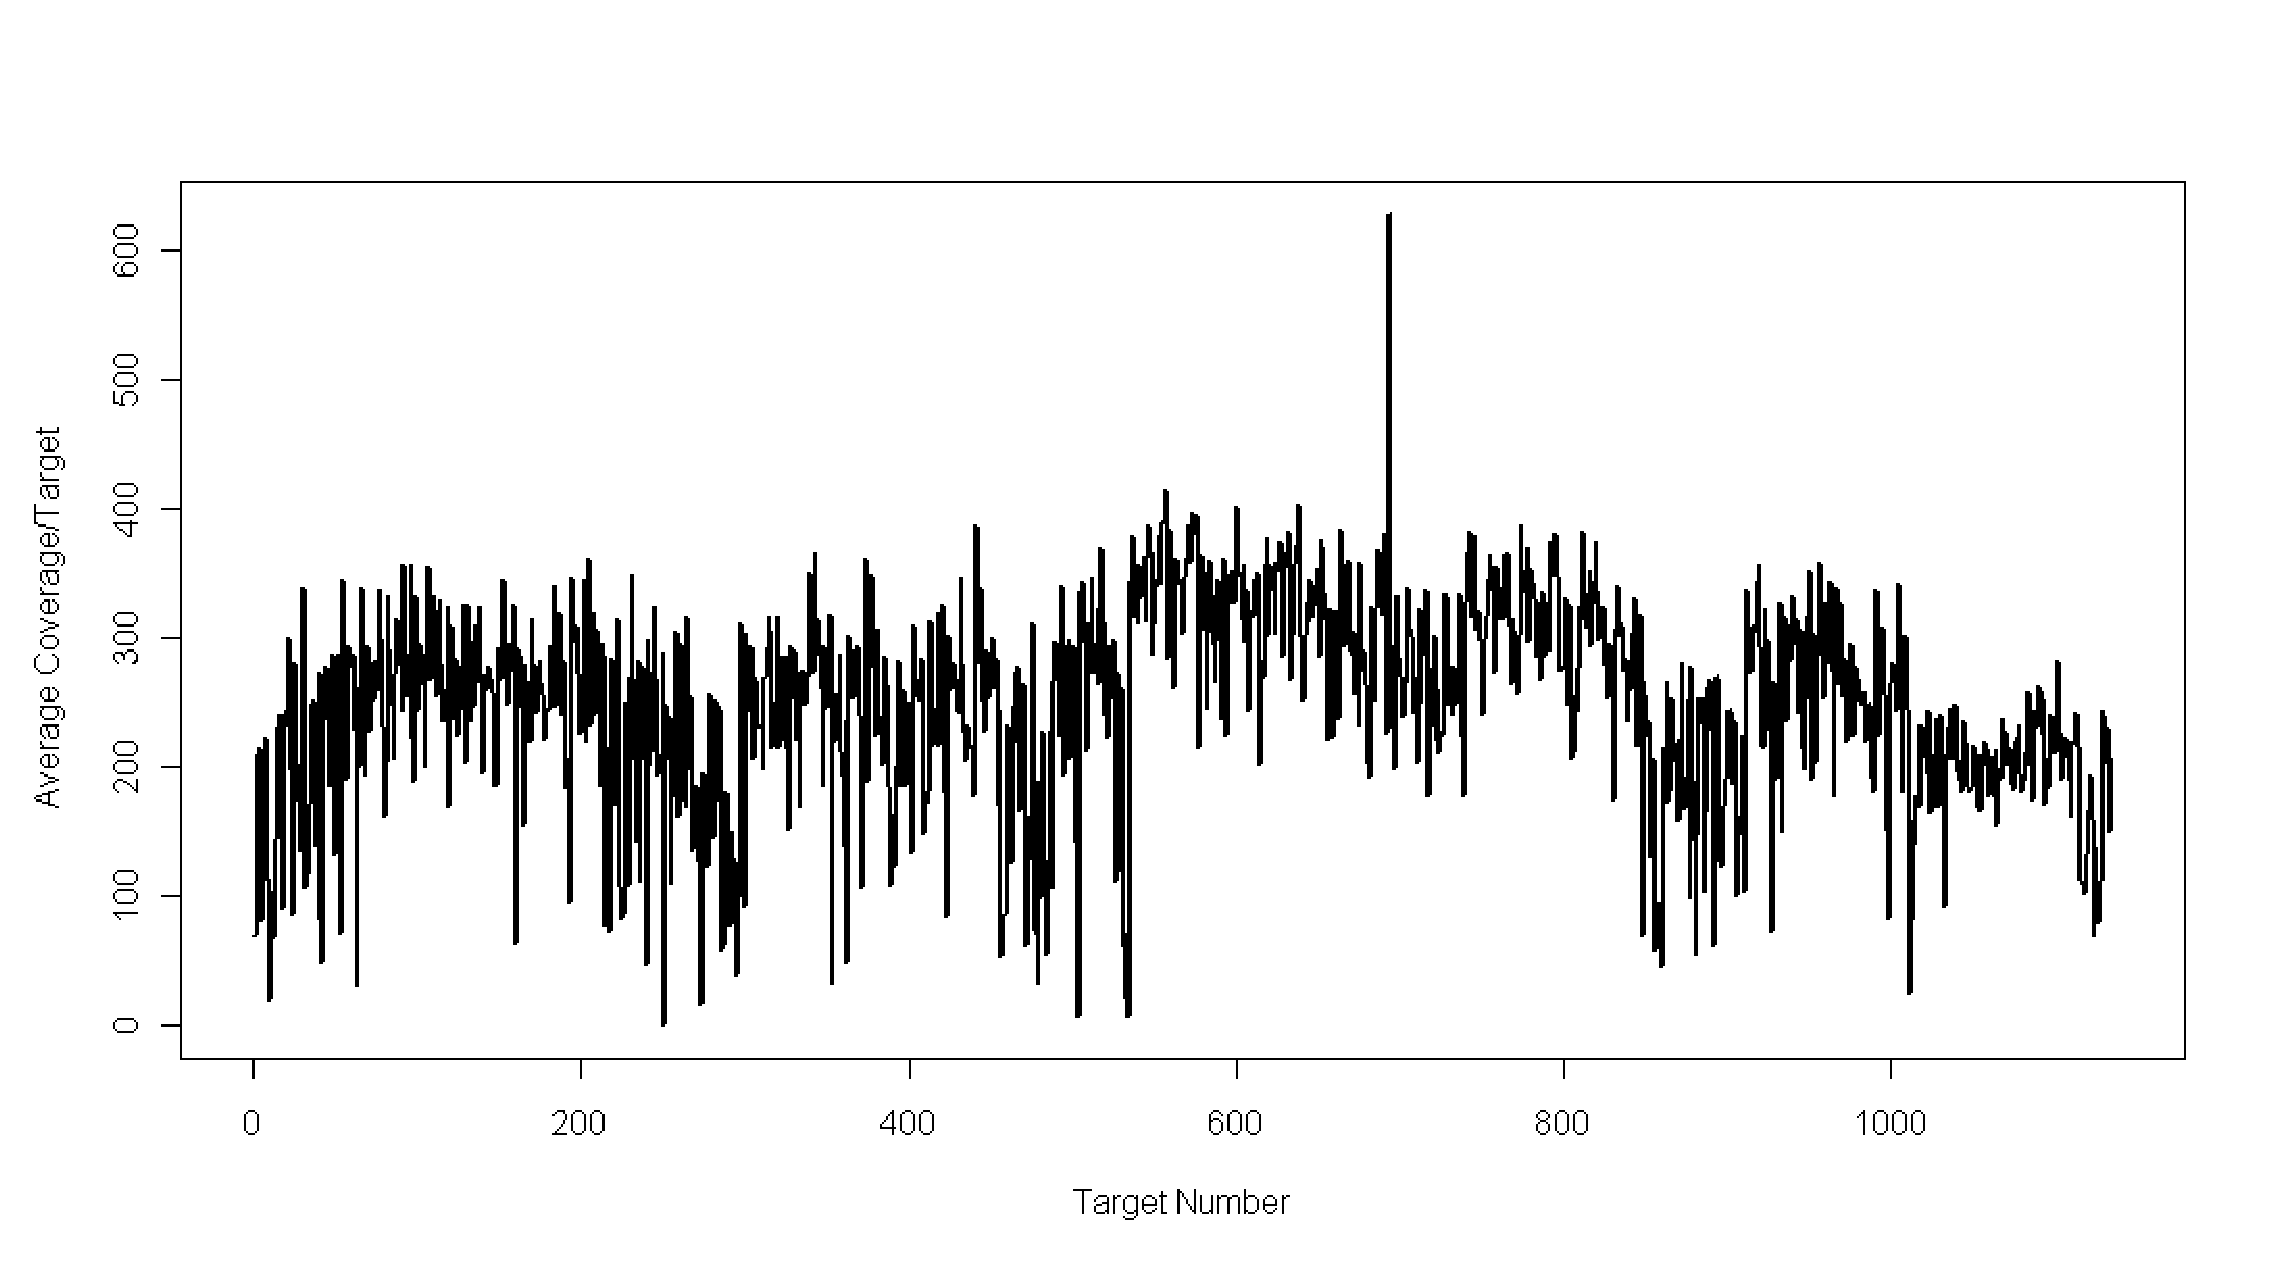
\includegraphics[width=1.0\linewidth]{img/SNP_Indel_Fig1}
	\caption[Average coverage per exon cardiomyopathy 48 gene panel]{Average coverage obtained from 22 different samples of all exon (1,133 exons) and exon/intron junctions ({$\pm$}20 bp) of 48 genes potentially involved in cardiomyopathy. 99\% of the targets show an average coverage of $\ge$30$\times$}
	\label{fig:SNP_Indel_Fig1}
\end{figure}

\begin{figure}[!ht]
	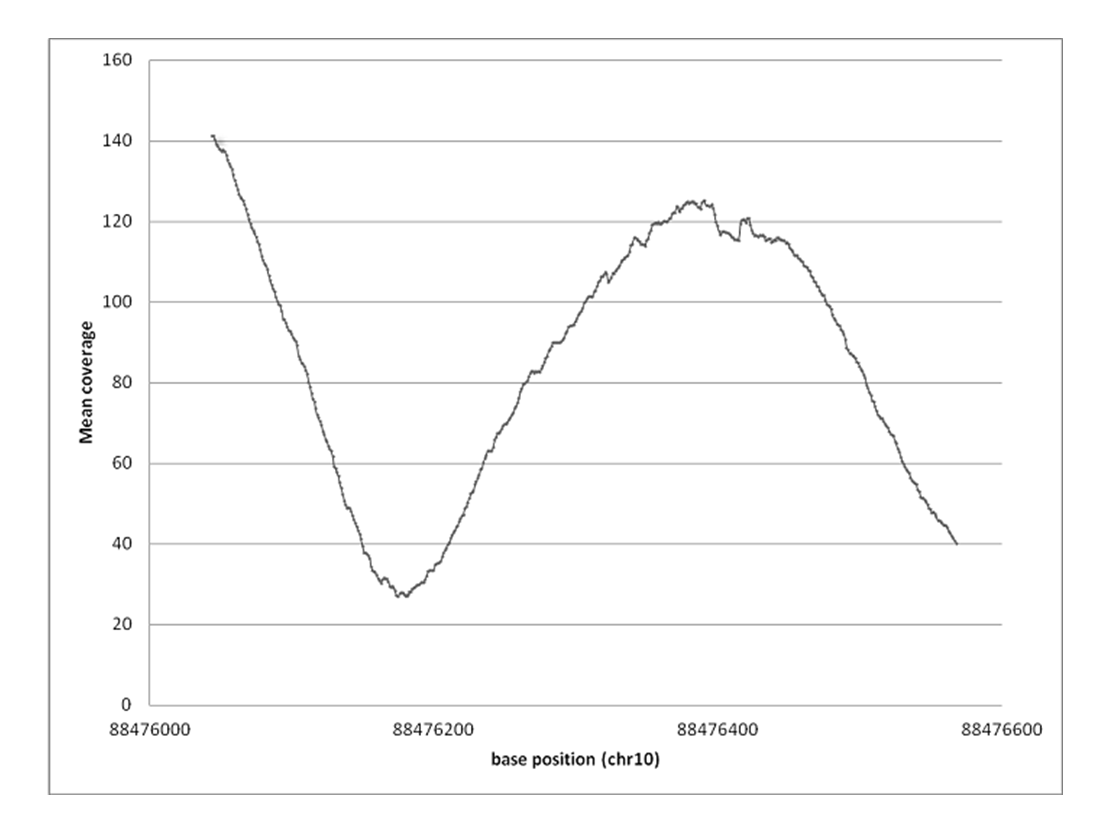
\includegraphics[width=1.0\linewidth]{img/SNP_Indel_Fig2}
	\caption[Coverage profile of single target \textit{LDB3} exon 9]{Coverage of one target, exon 9 of the \textit{LBD3} gene on chromosome 10 (NCBI build 37, UCSC hg19), representing one region with a coverage  $\le$30 in one patient.}
	\label{fig:SNP_Indel_Fig2}
\end{figure}


\begin{table}[!ht] %the []!ht] is to force the footnotes on the same page as the table
	\caption[Overview of the Sequence Performance for the Validation Runs]{\label{table:SNP_Indel_performance} Overview of the Sequence Performance for the Validation Runs}
	\tiny
	\resizebox{\linewidth}{!}{\begin{tabulary}{\linewidth}{p{3cm}p{2cm}p{2cm}p{2cm}}
			& Run 1 & Run 2 & Average of both runs \\
			\hline
			\rule{0pt}{1ex} Cluster density (k/mm\textsuperscript{2}) & 1,289 & 1,119 & 1,204  \\
			\rule{0pt}{1ex} \% Cluster PF & 89.3 & 94.6 & 92.0  \\
			\rule{0pt}{1ex} Q30 & 80.3 & 83.9 & 82.1  \\
			\rule{0pt}{1ex} Total reads & 17,168,243 & 15,788,049 & 16,478,146  \\
			\rule{0pt}{1ex} Matched reads & 16,414,062 & 15,186,556 & 15,800,309  \\
			\rule{0pt}{1ex} \% reads in .fasta file aligned & 96 & 96 & 96  \\
			\rule{0pt}{1ex} Mean mean coverage targets & 246 & 251 & 248  \\
			\rule{0pt}{1ex} Mean min coverage targets & 166 & 179 & 173  \\
			\rule{0pt}{1ex} Mean max coverage targets & 299 & 297 & 298  \\
			\rule{0pt}{1ex} \%Targets Mean {\textless}30 & 0.6 & 0.9 & 0.7  \\
			\rule{0pt}{1ex} \%Targets Mean {\textgreater}30 & 99.4 & 99.1 & 99.3  \\
			\rule{0pt}{1ex} \%Targets Min {\textless}30 & 2.6 & 2.5 & 2.6 \\
			\rule{0pt}{1ex} \%Targets Min {\textgreater}30 & 97.4 & 97.5 & 97.4  \\
			\rule{0pt}{1ex} \%Targets Max {\textless}30 & 0.4 & 0.7 & 0.5  \\
			\rule{0pt}{1ex} \%Targets Max {\textgreater}30 & 99.6 & 99.3 & 99.5  \\															
			\hline
	\end{tabulary}}
\end{table}


\subsubsection{Specificity and sensitivity of targeted NGS: confirmation of SS variants}
In previous SS analyses, a total of 90 variants in 14 different genes had been identified in the 24 patients used for validation (2 runs). 
All these variants were also detected with our targeted NGS approach applying the Agilent SureSelect kit (Fig. \ref{fig:SNP_Indel_Fig3}) and resulting in no false negatives. 
This included 84 substitutions and six indels (four deletions, two insertions). 
No additional variants were identified in these genes, comprising 55,784 bp. 
We therefore concluded that for these 24 samples there was full concordance with the SS results.

\begin{figure}[!ht]
	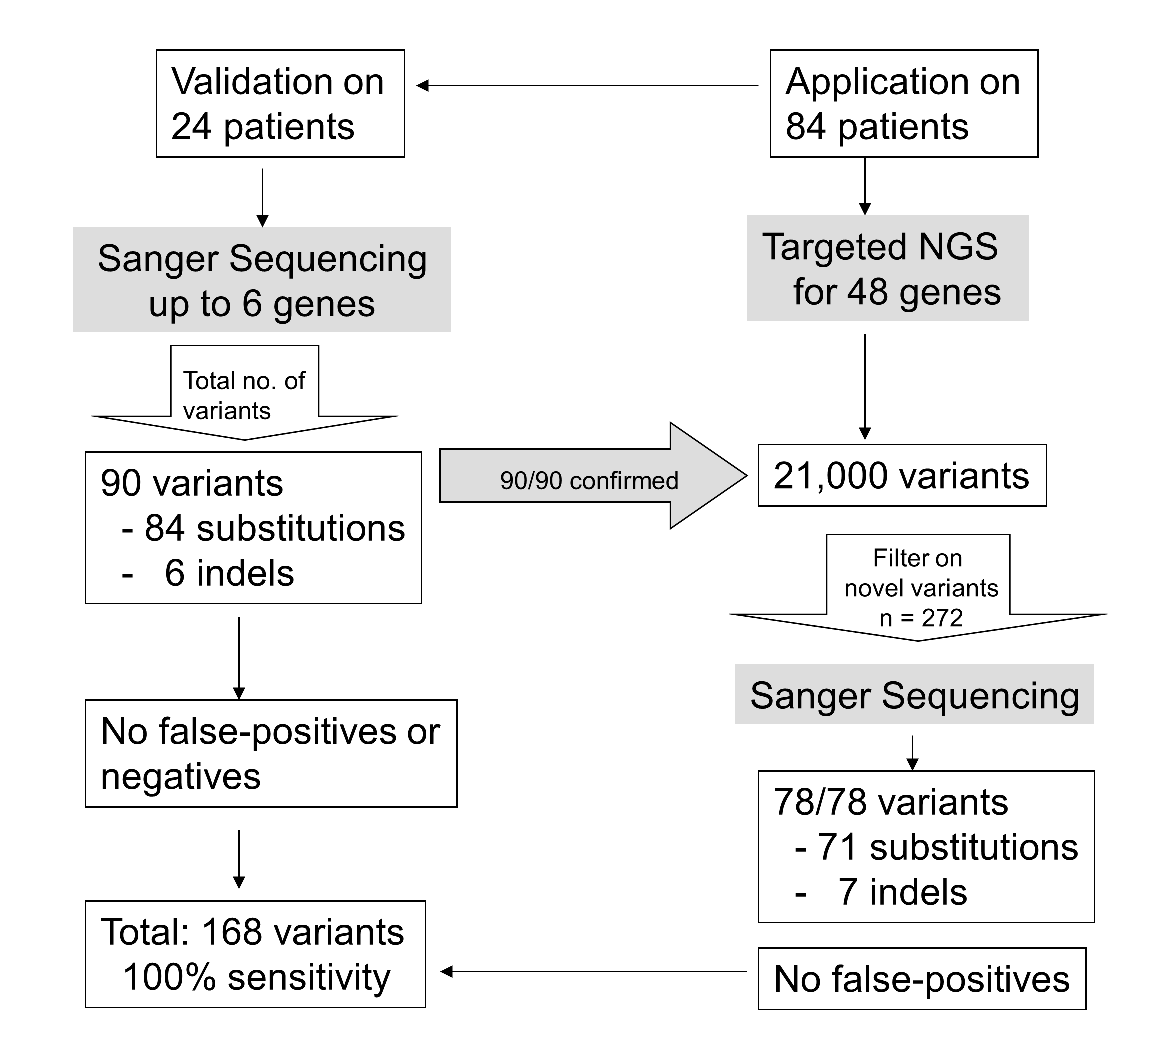
\includegraphics[width=1.0\linewidth]{img/SNP_Indel_Fig3}
	\caption[Summary of the results of our confirmation analyses]{Summary of the results of our confirmation analyses.}
\label{fig:SNP_Indel_Fig3}
\end{figure}

\subsection{Application Phase}

\subsubsection{Sequence specificity of targeted NGS: confirmation of NGS variants}
Using targeted NGS of 48 genes, approximately 21,000 variants were identified in 84 unique patients (Fig. \ref{fig:SNP_Indel_Fig3}), including the 90 variants that had been previously detected with SS. 
Of these variants, 272 were novel (245 substitutions, 27 indels). 
On average, we identified three novel variants per patient. 
For validationwith SS, 78 out of the 272 novel variants were selected, including detected indels (n = 7). 
The largest deletion comprised 18 bp and the largest insertion 8 bp. 
Notably, of the 71 substitutions, one was initially not confirmed by SS. 
This could be explained by the presence of a SNP in the primer binding site of the forward primer. 
A subsequent SS experiment, in which an alternative set of primers was used, did confirm the presence of this variant. 
In summary, a total of 168 variants were confirmed with SS. 
Based on these data, we reached a 100\% sensitivity (at 95\% confidence 97.76\%–100\%) \cite{Waerden_1957} with the NGS targeted approach.

\subsubsection{Diagnostic yield}
Applying this targeted NGS strategy, our first results indicate that the diagnostic yield is significantly improved from 15\% to about 40\%,mostly for DCM. 
However, this is based on small numbers of samples and the increase in yield may be even higher if this strategy is applied on a regular basis for larger series. 
Where regular routine diagnostics involves stepwise testing of up to about 10 different genes (which can easily take more than 1 year to complete), using targeted NGS of entire gene-panels on the MiSeq sequencer could theoretically provide reporting times of no more than 2 weeks. 
At this stage, we are aiming for reporting times of 4–6 weeks, a huge improvement compared with current diagnostic services.

\subsection{Reproducibility of Targeted NGS}
The entire procedure was performed twice for five samples, including sequencing in different runs. 
On average, 231 variants (198– 268) were detected per sample, and on average, 10 unique variants (8–14) were differently reported between the two analyses of identical samples. 
In total, 1,007 variants were detected and 51 of these were differently reported in the two separate analyses of the same sample resulting in a nonconcordance rate of 0.00315\% according to the number of sequenced bp (five times 323,651 bp of the targeted NGS kit). 
These differences can be attributed to three underlying causes: (1) in 12 out of 51 cases this was due to coverage differences, which meant variants were either not reported because of a too low coverage or reported when the coverage was just above threshold levels using the default settings; (2) in 24 out of 51 cases this was explained by alignment problems due to poly-T/A stretches, resulting in different annotating of the same variant; and (3) 15 out of 51 were due to differences in heterozygote levels, which meant variants that were present in {\textless}20\% of reads were not reported. 
Variants that fall within the first two categories are “true variants” that were either missed or reported as the result of analysis software settings or limitations. 
In contrast, variants in the third category most likely represent recurring technical artefacts, as all were repeatedly reported in a significant number of patients and in different runs, but were nonetheless not reported in the dbSNP and/or 1000 Genomes databases. 
Considering the artefacts as potential false positives the technical specificity is 0.0009269\%. 
In our future bioinformatic analyses, we will filter for the variants of the third category during our selection for potentially interesting variants, in addition to other filtering steps.

\section{Discussion}\label{discussion}
We present the validation of a targeted resequencing method for cardiomyopathy-associated genes and our results support its implementation in routine diagnostics. 
In this study, all the 168 variants identified by our NGS-approach were confirmed with SS (Fig.  \ref{fig:SNP_Indel_Fig3}). 
The variants included deletions up to 18 bp and insertions up to 8 bp. 
No false-negative or false-positive results were obtained for variants selected for confirmation. 
We therefore conclude that, at a coverage of at least 30 times per nucleotide, the performance of our procedure is comparable with SS. 
ES is likely to become the most commonly used tool for identifying genes in Mendelian diseases in the coming years \cite{Gilissen_2012}.
This approach has been shown to be successful in cases of rare monogenetic disorders \cite{Gilissen_2010,Hoischen_2010,Ng_2010} and of intellectual disability \cite{Vissers_2010}. 
However, as demonstrated by Gilissen et al. (2012)\cite{Gilissen_2012}, 2128 (5.7\%) of 37,424 disease-causing variant positions from the Human Genome Mutation Database are not covered with the 50Mb SureSelect ES kit (Agilent Technologies, Inc.). 
From our experience, we know that all the 48 genes we targeted are covered by probes in the 50Mb ES kit. 
However, the coverage performance varied significantly between exons within a gene and between different genes, and for some regions the coverage was {\textless}20 times, too low for reliable variant detection. 
This is exemplified by the \textsl{TTN} gene. 
Recently, Herman et al. (2012)\cite{Herman_2012} showed that \textsl{TTN} truncating mutations are a common cause of DCM, occurring in approximately 25\% of familial cases of idiopathic DCM and in 18\% of sporadic cases. 
From our ES data, we have calculated the average coverage per target for the coding regions of \textsl{TTN}. 
We found that 7\% of the targets sequenced had an average coverage of $\le$20 times (around 25 exons) and among those, 12 exons showed an average coverage of $\le$10 times. 
It is therefore very likely we would miss clinically relevant variants in these regions of low coverage. 
In contrast, the targeted region of the \textsl{TTN} gene in our designed kit shows a 100\% coverage for all exons and the respective nucleotides were all covered $\ge$30 times, with a high reproducibility between different samples. 
We therefore decided to continue developing our targeted resequencing method to overcome the shortcomings of incomplete representation and coverage of exons in ES experiments. 
The first prerequisite for high sensitivity of a NGS method is the development of a well-designed enrichment kit. 
We chose to use the SureSelect kit (Agilent Technologies, Inc.) as the e-Array programme used for kit design offered flexibility in optimizing the respective probe design. 
The number of tilings of each target can be chosen and extra baits can be added for GC-rich targets to increase coverage. 
A theoretical 100\% representation was reached for all of our targets. 
Based on our data, the theoretical representation given by e-Array is indicative for the actual coverage. 
Because the cost of a targeted custom-made enrichment kit is rather high, a good prediction of the coverage is an advantage before ordering such a kit for diagnostic use. 
The second prerequisite is high coverage of preferably all the targets. 
Setting the threshold at a coverage $\ge$30, we found only 50 targets out of the 1,134 with less coverage of the nucleotides, mostly in a part of the respective targets. 
We therefore decided that, parallel to targeted NGS, we will perform SS for targets with a low coverage from those genes of which the clinical relevance is uncontested (e.g., \textsl{MYH7}, \textsl{TNNI3} or \textsl{MYBPC3} for HCM; \textsl{LMNA}, \textsl{MYH7} or \textsl{MYBPC3} for DCM; and \textsl{PKP2} for ARVC) to ensure complete coverage of the respective amplicons (see Table \ref{table:SNP_Indel_recommendations} for general recommendations). 

\begin{table}[!ht] %the []!ht] is to force the footnotes on the same page as the table
	\caption[Diagnostic Workflow and Implementation Guidelines]{\label{table:SNP_Indel_recommendations} Resulting Diagnostic Workflow and Implementation Guidelines}
	\tiny
	\resizebox{\linewidth}{!}{\begin{tabulary}{\linewidth}{p{3cm}p{6cm}}
			Workflow & Recommendations  \\
			\hline
			\rule{0pt}{1ex}  & \\
			\rule{0pt}{1ex} Enrichtment kit construction & Theoretically 100\% horizontal and vertical coverage of all targets  \\
			\rule{0pt}{1ex} Sample preparation &  \\
			\rule{0pt}{1ex} Days 1-3 & Automated, that is, using a Bravo or Caliper robot (Agilent Technologies, Inc./Caliper Life Sciences, Hopkinton, MA)  \\
			\rule{0pt}{1ex} Sample Enrichment & Bar-coding samples to a theoretical mean coverage of 250 for all targets resulting in a coverage of at least 30 per nucleotide in p8\% of targets  \\
			\rule{0pt}{1ex} Days 4-6 & Avaiding sample-mix-up by spiking unique DNA sequences before the procedure or including a limited SNP analysis for each individual patient  \\
			\rule{0pt}{1ex} Sequencing on bench-top machine & 80\% of the reads with Q30  \\
			\rule{0pt}{1ex} Days 7-8 &  \\
			\rule{0pt}{1ex} Data analysis & \\
			\rule{0pt}{1ex} Days 8-10 & Minimal coverage of 30 per nucleotide   \\
			\rule{0pt}{1ex}  & In house (control) variant database for filtering \\
			\rule{0pt}{1ex}  & A predifined variant filtering precedure, preferably automated in software programmes like the NGS bench lab from CARTAGENIA (Leuven, Belgium)\footnotemark[1]  \\
			\rule{0pt}{1ex} Confirmation with Sanger Sequencing &  \\
			\rule{0pt}{1ex} Days 11-20 & Obsolete at a coverage of {\textgreater}30 per nucleotide \\
			\rule{0pt}{1ex}  & Coverage of targets structurally below 20: Sanger sequencing in parallel with NGS \\
			\rule{0pt}{1ex}  & Incidental coverage below 20: Sanger sequencing depending on the target's clinical relevance \\
			\rule{0pt}{1ex}  & Coverage between 20 and 30: visual inspection, Sanger sequencing of novel variants  \\
			\rule{0pt}{1ex} Total turn-around time & 21 days  \\															
			\hline
	\end{tabulary}}
\end{table}
\addtocounter{footnote}{1}
\footnotetext{ Basepair position according to NCBI build 37}

Valencia et al. (2012)\cite{Valencia_2012} developed a SureSelect enrichment kit for congenital muscular dystrophy for 321 targets (12 genes) and 95\% of them had a coverage of at least 20. 
According to their data, the coverage was below 20 times for two genes due to a high GC content. 
In contrast, our kit represents amuch better coverage (99\% covered more than 30 times). 
There are several explanations for this difference, for instance the tiling of the baits, differences in the overall GC content, or the number of pooled patients, which make a good comparison difficult. 
In our approach, 12 samples were pooled based on the size of the enrichment kit to reach a coverage of at least 30 times per basepair for most of the targets. 
Because no false-positive or -negative results were detected, this would seem to be a safe threshold. One could even consider whether more than 12 patients could be pooled or the coverage threshold reduced to {\textgreater}20 times instead of {\textgreater}30 times. 
In Table \ref{table:SNP_Indel_recommendations}, we give some general recommendations on the clinical laboratory implementation and quality assessment of targeted resequencing methods. 
These recommendations are in line with the general guidelines for assuring the quality of NGS in clinical laboratory practice formulated by the national workgroup of the US Centers for Disease Control and Prevention \cite{Gargis_2012}.
A 100\% sensitivity (95\% confidence: 97.76\%–100\%) was reached with our approach and a specificity of nearly 100\% (0.00315\% false positive). 
Gowrisankar et al. (2010)\cite{Gowrisankar_2010} reported a false-positive rate of 0.011 $\pm$0.002\%, close to 100\% specificity for 41,475 bp using an Illumina GAII sequencing machine and targeted resequencing of 19 DCM genes. 
However, four out of the 160 basepair substitutions and three out of 31 indels were missed, including one 18 bp duplication. 
The basepair substitutions were missed because of insufficient coverage ({\textless}30 times), whereas the indels were likely missed due to sequencing of short read lengths (36 bp). 
In our approach, 151 bp reads were used and we were able to detect an 18 bp deletion, the largest indel detected in our study. 
In total, 17 indels detected were confirmed with SS, but it is debatable how many and which type of indels should be confirmed by SS for proper validation. 
Depending on the gene panel to be sequenced, it seems obvious to choose patients with the largest known indels for validation. 
Gowrisankar et al. (2010)\cite{Gowrisankar_2010} recently reported an 18 bp duplication and Herman et al. (2012)\cite{Herman_2012} a 13 bp deletion in the titin gene, which seem to be the largest indels associated with cardiomyopathies so far. 
As indels of that size were detected in our procedure, we are convinced we can retain 100\% sensitivity. 
Moreover, according to our results, we would have missed one variant with SS due to a SNP in the primer sequence. 
This suggests that resequencing after hybridization-based enrichment of targets may even outperform SS. 
The importance of longer read lengths was underscored by the results of Voelkerding et al. (2010)\cite{Voelkerding_2010}. 
They performed SureSelect enrichment for 12 genes responsible for congenital muscular dystrophy in combination with sequencing on a SOLiD machine. 
Two out of the 34 identified variants were not confirmed with SS because of sequence read misalignment between two closely related genes. 
As a probe based method, not only targeted sequences but also highly homologous pseudogenes and other homologous sequences, such as those present in gene families and domain analogs will be captured \cite{Coonrod_2012}. 
Highly homologous sequences coalign to the reference sequence. 
However, it is uncertain to what extent regions of high-homology may negatively affect the sensitivity and specificity. 
In general, construction of a unique tiled bait library using differences in the neighboring intron sequences and eventually longer paired end reads can reduce this problem. 
The reproducibility of our procedure was tested by repeating the procedure for five samples. 
The 99.99685\% concordance of all detected variants demonstrates the high performance of our targeted enrichment and MiSeq resequencing method. 
Apart from low coverage an alignment problem due to poly A/T stretches resulted in discrepancies. 
However, these variants will not result in false positives. 
Discrepancies due to differences in the heterozygote level of 20\% might be considered as technical false positives (0.0009269\%). 
However, according to our analyses criteria we would have filtered these variants out. 
In summary, the differences seen between the separate analyses of the five repeated samples were due to bioinformatic threshold and annotation settings and not due to technical limitations. 
Variants with an allelic imbalance need careful follow up. 
This is in line with the first report on a MiSeq-based sequencing method in which drafting genomic sequences of E. coli resulted in an error rate of 0.1 substitutions per 100 bases and a near absence of indel errors\cite{Loman_2012}. 
This, together with the almost 100\% sensitivity and specificity of our results, raises the question whether a variant still needs to be confirmed with SS, as is often daily practice in clinical diagnostics at the moment. Zhang et al. (2012)\cite{Zhang_2012} felt it was necessary for two reasons: first, to remove incorrect calls due to experimental errors, and second, to confirm a diagnosis. 
However, as they discussed, confirmation becomes burdensome or impossible when a large number of novel variants need to be confirmed and this would result in long turn-around times. 
We therefore propose to refrain from confirming results with SS as long as the coverage is {\textgreater}30 times per nucleotide. 
In addition, targets that are not covered or badly covered can either be excluded from the final report or SS of these targets can be performed in parallel. 
At a coverage between 30 and 20 times, visual inspection of the regions is recommended (see Table \ref{table:SNP_Indel_recommendations} for general recommendations).

\section{Conclusion}
Our data convincingly demonstrate that targeted NGS of a disease-specific subset of genes can be reliably implemented as a stand-alone diagnostic test.

\section{Acknowledgments}\label{Acknowledgments} 
We thank Jackie Senior for editorial advice.


\subsubsection{Disclosure Statement} 
The authors declare no conflict of interest.


\chapter[CoNVaDING: Single Exon Variation Detection in NGS data]{CoNVaDING: Single Exon Variation Detection in Targeted NGS Data}
\chaptermark{CoNVaDING: CNV detection in NGS data}
\label{chap:CoNVaDING}

{ \Large \leftwatermark{
		\put(-67,-66.5){ 1 }
		\put(-67,-91.5){ 2 }
		\put(-76.5,-125){
\includegraphics[scale=0.8]{img/thumbindex.eps}} \put(-67,-116.5){ {\color{white} 3 }}
		\put(-67,-141.5){ 4 }
		\put(-67,-166.5){ 5 }
		\put(-67,-191.5){ 6 }
		\put(-67,-216.5){ 7 }
		\put(-67,-241.5){ 8 }
		\put(-67,-266.5){ 9 }
		\put(-67,-291.5){ 10 }
		\put(-67,-316.5){ 11 }
	} \rightwatermark{
		\put(350.5,-66.5){ 1 }
		\put(350.5,-91.5){ 2 }
		\put(346.5,-125){
\includegraphics[scale=0.8]{img/thumbindex.eps}} \put(350.5,-116.5){ {\color{white} 3 }}
		\put(350.5,-141.5){ 4 }
		\put(350.5,-166.5){ 5 }
		\put(350.5,-191.5){ 6 }
		\put(350.5,-216.5){ 7 }
		\put(350.5,-241.5){ 8 }
		\put(350.5,-266.5){ 9 }
		\put(350.5,-291.5){ 10 }
		\put(350.5,-316.5){ 11 }
}}

\hfill \underline{Human Mutation} 2016;37(5):457-464.

\hfill DOI: \href{https://doi.org/10.1002/humu.22969}{10.1002/humu.22969}

\hfill PubMed ID: \href{https://www.ncbi.nlm.nih.gov/pubmed/26864275}{26864275}

\newpage

\noindent
L.F. Johansson\textsuperscript{1,2,*}, F. van Dijk\textsuperscript{1,2,*}, E.N. de Boer\textsuperscript{1}, K.K. van Dijk-Bos\textsuperscript{1}, J.D. Jongbloed\textsuperscript{1}, A.H. van der Hout\textsuperscript{1}, H. Westers\textsuperscript{1}, R.J. Sinke\textsuperscript{1}, M.A. Swertz\textsuperscript{1,2}, R.H. Sijmons\textsuperscript{1},B. Sikkema-Raddatz\textsuperscript{1}  \\

\noindent
1. University of Groningen, University Medical Center Groningen, Department of Genetics, Groningen, The Netherlands\\
2. University of Groningen, University Medical Center Groningen, Genomics Coordination Center, Groningen, The Netherlands\\


\noindent
Received 2015 Nov 26; Accepted revised manuscript 2016 Jan 27; Published online 2016 Feb 10.
\\~\\
* Contributed equally


\section*{Abstract}\label{abstract}
We have developed a tool for detecting single exon copy-number variations (CNVs) in targeted next-generation sequencing data: CoNVaDING (Copy Number Variation Detection In Next-generation sequencing Gene panels).
CoNVaDING includes a stringent quality control (QC) metric, that excludes or flags low-quality exons. 
Since this QC shows exactly which exons can be reliably analyzed and which exons are in need of an alternative analysis method, CoNVaDING is not only useful for CNV detection in a research setting, but also in clinical diagnostics. 
During the validation phase, CoNVaDING detected all known CNVs in high-quality targets in 320 samples analyzed, giving 100\% sensitivity and 99.998\% specificity for 308,574 exons. 
CoNVaDING outperforms existing tools by exhibiting a higher sensitivity and specificity and by precisely identifying low-quality samples and regions. 

\section{Introduction}\label{introduction}
Several methods for detecting exon deletion and duplication using next-generation sequencing (NGS) have been reported for whole genome \cite{Zhao_2013,Gilissen_2014,Francioli_2014} and whole gene sequencing data \cite{Wang_2014}. 
With the exception of those using read depth approaches, these methods rely on information from sequence reads spanning the breakpoints. 
For targeted NGS data, however, only a read depth approach can be successfully applied \cite{Tan_2014}. 
Existing tools using this approach are XHMM \cite{Fromer_2012}, CoNIFER \cite{Krumm_2012}, CONTRA \cite{Li_2012}, and CODEX \cite{Jiang_2015}. 
All four consider all control samples equally informative even though there are sample to sample variations caused by differences in PCR and capturing efficiency, which lead to variations in coverage patterns that complicate the determination of expected read depths \cite{Aird_2011}\cite{Zhao_2013}. 
In the four existing tools, this increases the risk of false- negative (FN) or false-positive (FP) results for exons with a high read depth variation, giving either a low sensitivity and specificity for single exon copy-number variation (CNV) detection or limiting the analysis to detection of variations that span multiple exons. 
This has meant that, until now, additional experiments were needed to identify single exon CNVs, including multiplex ligation-dependent probe amplification (MLPA) \cite{Schouten_2002}, Q-PCR \cite{Ebenazer_2013}, or array comparative hybridization \cite{Vasson_2013}. 
These additional experiments are, however, costly and usually only applied to genes known to frequently harbor deletions or duplications. 
To overcome this limitation, we have developed CoNVaDING, an analysis tool that not only detects single (and multiple) exon CNVs with high sensitivity and specificity, but also provides quality metrics for each sample that distinguish high-quality samples and targets from low-quality ones with a high risk of producing FP or FN results.

\section{Material and Methods}

\subsection{General Workflow CoNVaDING}
The CoNVaDING analysis consists of several steps to determine whether a deletion or duplication is present. 
CoNVaDING focuses on specified target regions (Fig. \ref{fig:CoNVaDING_Fig1}A) and utilizes control samples captured with the same gene panel for a read depth comparison. 
A strategy unique for CoNVaDING is that out of a set of available control samples, it selects only samples with a coverage pattern that is most similar to that of the sample analyzed (Fig. \ref{fig:CoNVaDING_Fig1}C). \
The selected control samples are therefore most informative for this specific sample. 
CoNVaDING then normalizes the data in two different ways in parallel in order to enable comparison between the sample and the control samples. The first normalization uses all targets or all autosomal targets within the sample (Fig. \ref{fig:CoNVaDING_Fig1}B) and the second uses all targets of the same gene (Fig. \ref{fig:CoNVaDING_Fig1}D). 
Based on the normalized data, the ratio of the normalized average read depth of the sample to that of the controlsanda distribution analysis using a Z-score are calculated for each target (Fig. \ref{fig:CoNVaDING_Fig1}E). 
Based on the calculated ratio and distributions, a prediction is made for each target to determine whether a CNV is present or not (Fig. \ref{fig:CoNVaDING_Fig1}F). 
The mathematical formulas used are described in the Supplemental methods.


\begin{figure}
	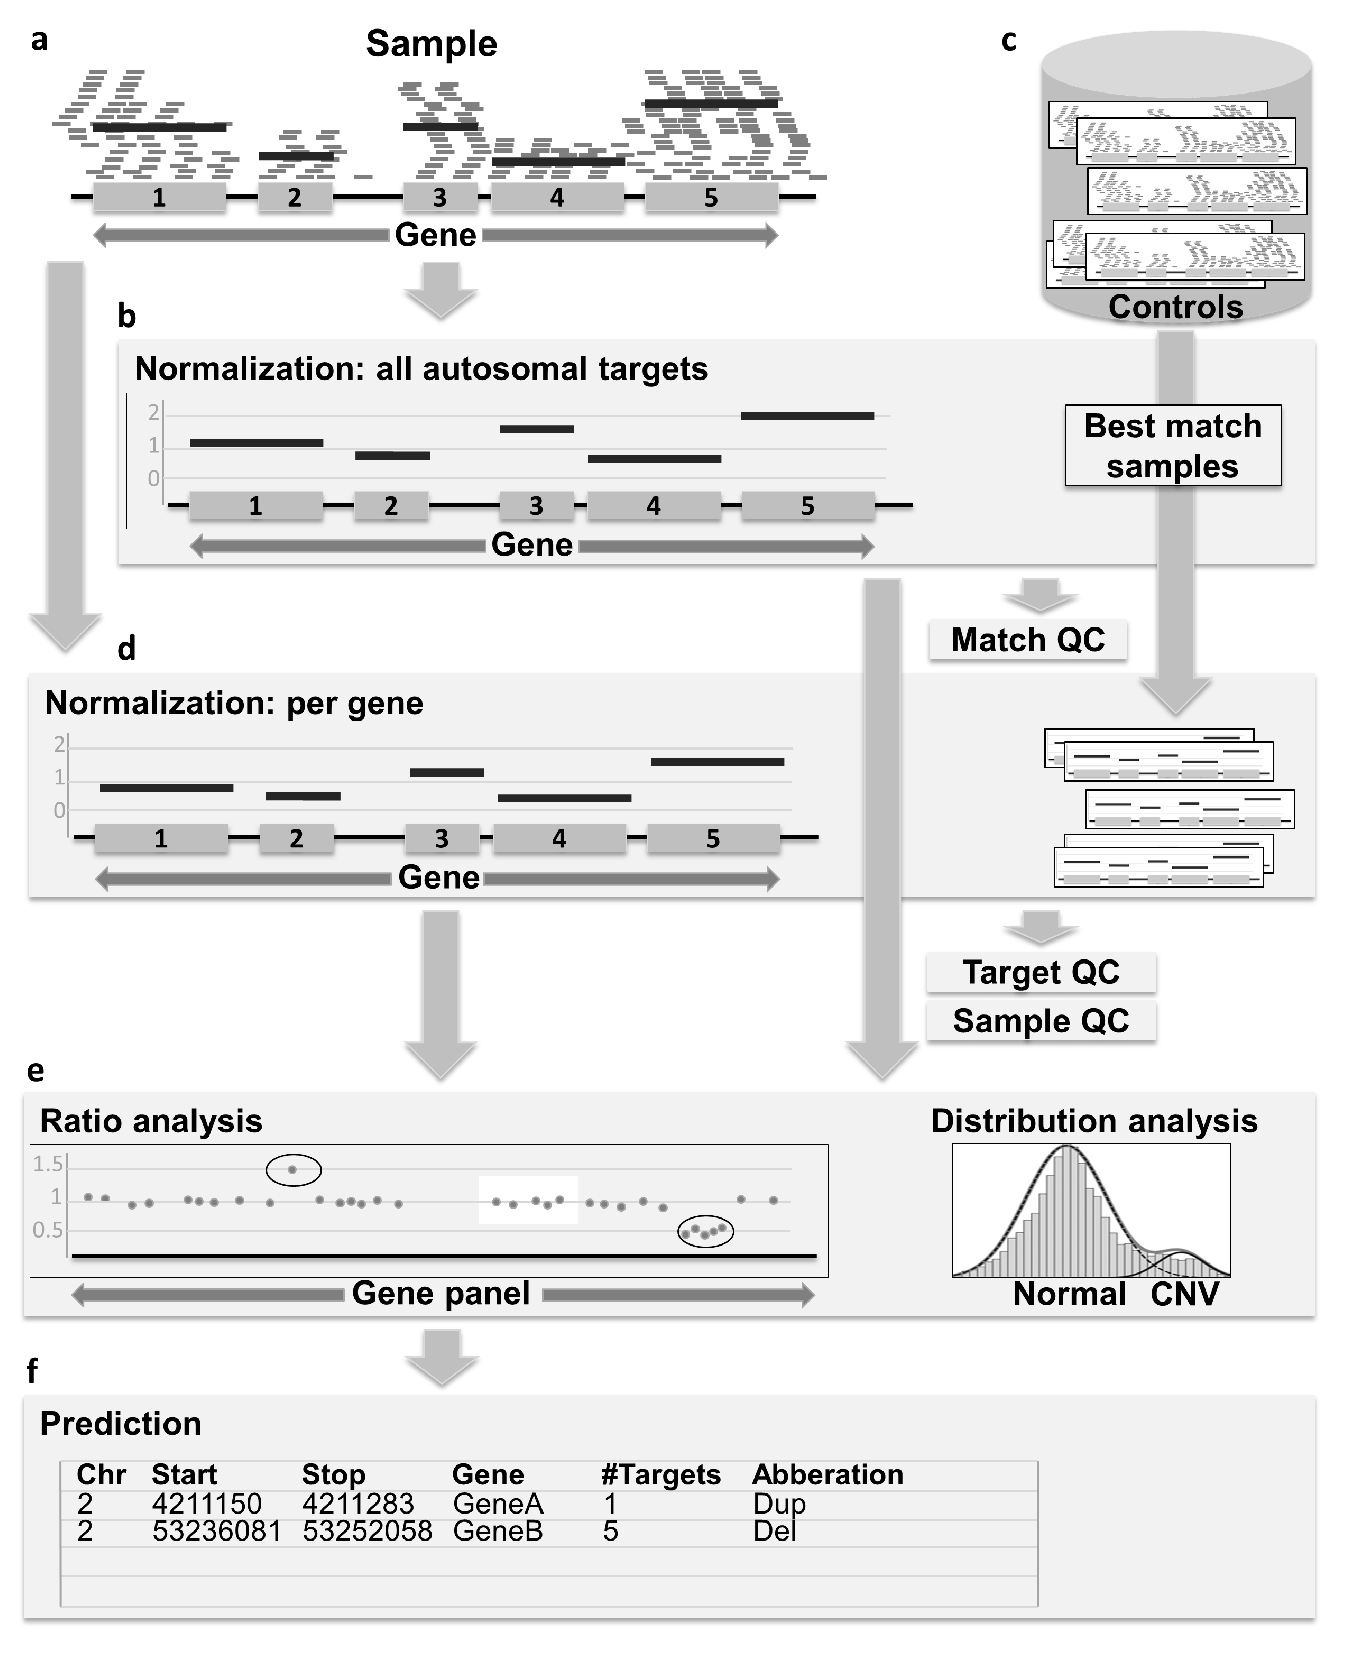
\includegraphics[width=1.0\linewidth]{img/CoNVaDING_Fig1}
	\caption[CoNVaDING workflow]{Caption next page.}
	\label{fig:CoNVaDING_Fig1}
\end{figure}
\addtocounter{figure}{-1}
\begin{figure}
\caption[]{(Previous page.) CoNVaDING workflow. A: For each specified target region, the average coverage is calculated for the analyzed sample. B: The sample is normalized using the average coverages of all autosomal targets. C: Out of a set of possible control samples, the samples showing the most similar coverage pattern are selected as control samples. The Match QC shows how well the control samples match the analyzed sample. D: All targets are alternatively normalized using the average coverages of targets belonging to the same gene. E: Based on the normalizations, a ratio and a distribution analysis are performed, showing the relative difference of the average coverages of the targets of the sample compared with those of the control samples. Target QC and Sample QC metrics are calculated showing the variability of each target and the complete sample. F: Based on the ratio and distribution analysis, a copy-number variation (CNV) prediction is made.}
\end{figure}

\subsection{Input Data}
CoNVaDING analysis starts with a list of targets that specify chromosome, start and stop position of the target and the exact gene the target belongs to. 
For each sample and the possible control samples, a BAM file containing aligned reads is also needed \cite{Li_2009}. 
Typically, targets specify the exonic regions ofwhich the gene panel consists of, or a subset thereof. 
After an optional removal of sequence duplicates, for each BAMfile, of all targets in the sample and in the possible control samples, the average depth of coverage is calculated (Fig. \ref{fig:CoNVaDING_Fig1}A).

\subsection{Control Group Selection}
CoNVaDING makes use of a set of possible control samples that should be produced using the same type of sample preparation and sequencing as the test sample. 
The control samples with the most similar overall coverage patterns are selected using a “match score” for each possible control sample. 
This match score is calculated by first correcting all samples for total read number difference, that is, dividing the average depth of coverage of the target by the mean average depth of coverage of all (autosomal) targets (typeAnormalization) (Fig. \ref{fig:CoNVaDING_Fig1}B). 
Subsequently, the absolute difference between the sample and each possible control sample is calculated for each target. 
For each possible control sample, the absolute differences are sorted from smallest to largest and the average absolute difference of the center 95\% targets, the match score, is calculated. 
A lower match score indicates a more similar overall coverage pattern and thus a more suitable control sample. The control samples with the lowest match scores are selected for further analysis (Fig. \ref{fig:CoNVaDING_Fig1}C). 
A minimum of 30 control samples is needed for analysis. 
An example of the characteristics of the selected control groups for two samples is shown in Figure \ref{fig:CoNVaDING_Fig2}.


\begin{figure}[!ht]
	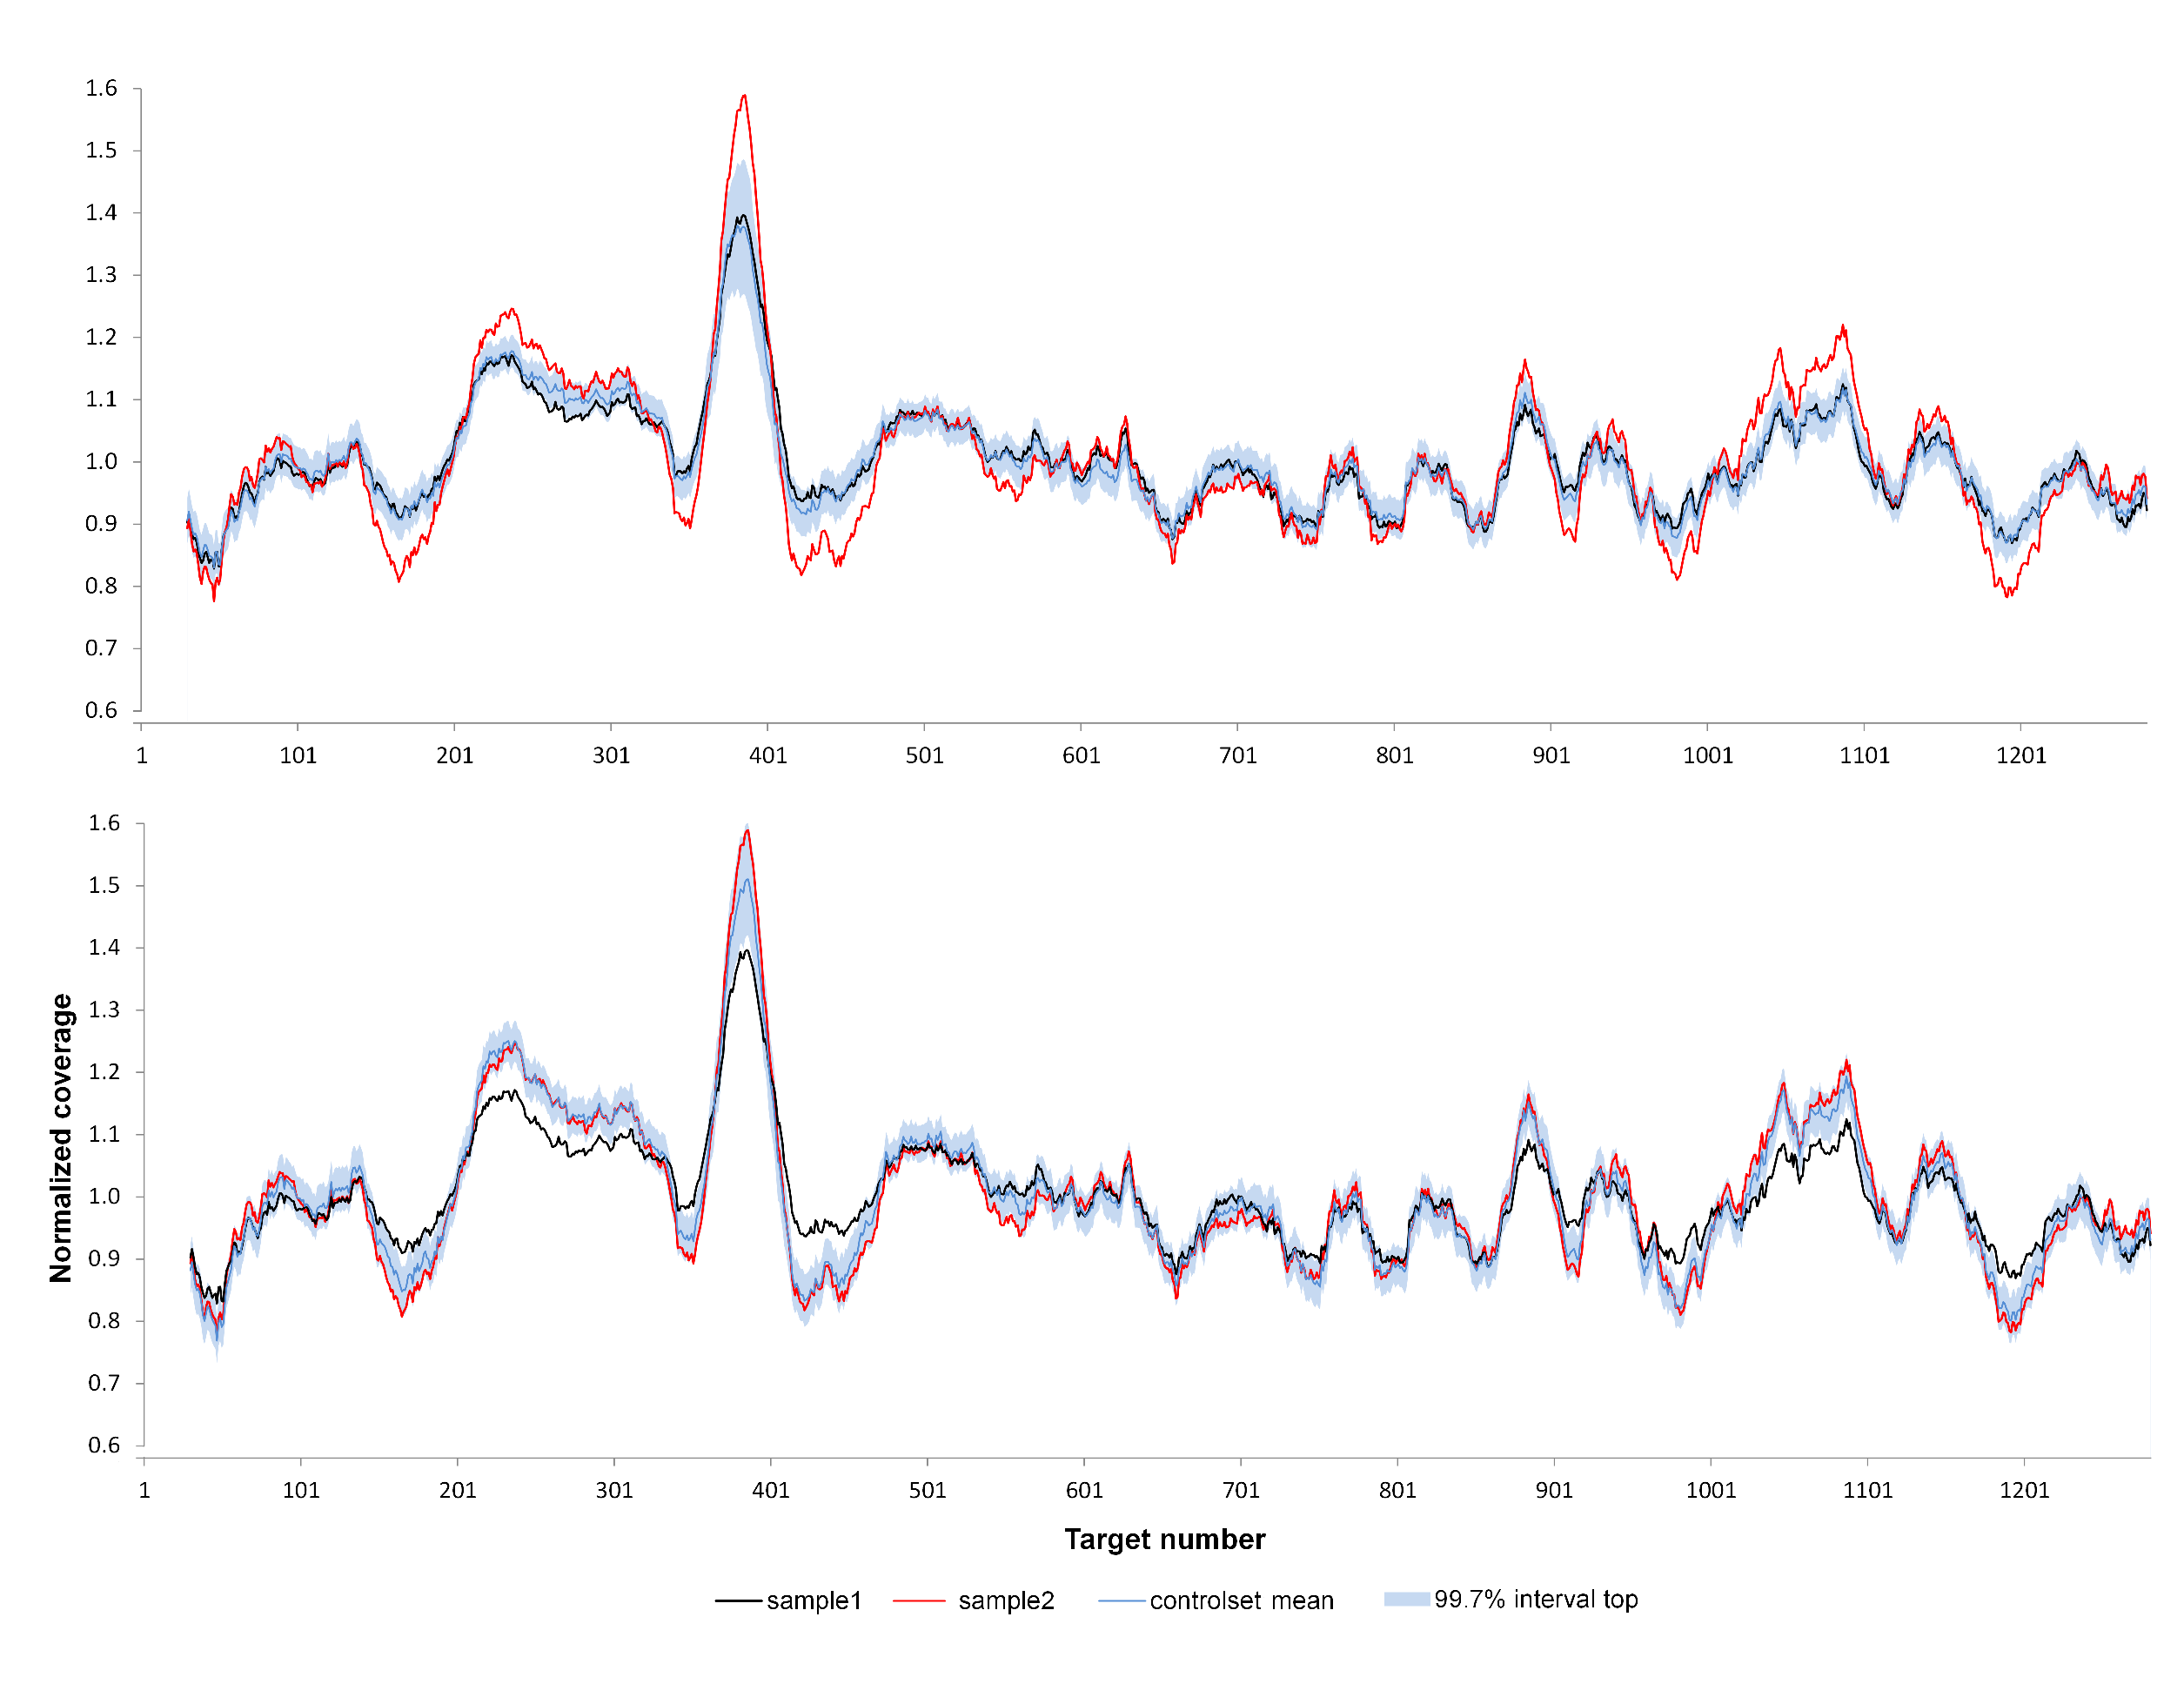
\includegraphics[width=1.0\linewidth]{img/CoNVaDING_Fig2}
	\caption[CoNVaDING match control group]{Both graphs show the moving average of the normalized coverage over 30 targets of two test samples (sample 1 [black continuous line] and sample 2 [red line line]) and the mean control group value of the 30 best matching normalized control samples (blue line line) with the 99.7\% confidence interval (light blue area area). In graph (A), the best-fitting control samples for sample 1 are selected as control group and in graph (B) the best-fitting control samples for sample 2 are selected. Both test samples fitwithin the 99.7\% confidence interval of their own best matching control group, but compared with the 99.7\% confidence interval of the other control group, there are overrepresented and underrepresented regions.}
	\label{fig:CoNVaDING_Fig2}
\end{figure}

\subsection{CNV Prediction Score Calculation}
After the control group selection, the selected control samples are used as a reference set. 
All samples are normalized to enable comparison between samples. Two types of analysis, the ratio score analysis and the distribution score analysis, are performed to determine determine the relative difference between the sample of interest and the selected control samples. 
Results of both calculations are combined and, together with quality metrics, are used to predict the presence of a CNV. 
Normalization within the sample is done in two different ways.
The first (type A normalization) is the normalization using all (autosomal) targets (Fig. \ref{fig:CoNVaDING_Fig1}B). 
The second (type B normalization) alternatively normalizes the read number of the targets by dividing the average depth of coverage of the target of interest by the mean average depth of coverage of all targets belonging to the same gene as the target (Fig. \ref{fig:CoNVaDING_Fig1}D).

\subsubsection{Ratio score}
The ratio score shows the ratio of the read depth of the sample to the expected read depth (Fig. \ref{fig:CoNVaDING_Fig1}E). 
This score is calculated for each target by dividing the type A normalized depth of coverage by the average type A normalized depth of coverage in the selected control samples. 
If no deletion or duplication is present, the sample of interest is expected to have the same normalized average depth of coverage as the selected control samples, a condition indicated by ratio scores close to 1.0. 
Deletions and duplications are expected to have a ratio of \textapprox0.5 and \textapprox1.5, respectively. Default cut-offs are set at a ratio below 0.65 for deletions and a ratio above 1.4 for duplications. 
Ratios below 0.10 or above 1.75 indicate homozygous deletions or amplifications, respectively. This is in concordancewith the cut-offs used in MLPA \cite{MRC_Holland_2014}, with the exception of the duplication threshold, which we increased from 1.3 to a more stringent 1.4 to improve specificity. Targets with an average coverage of 0 are excluded from further analysis.


\subsubsection{Distribution score}
The distribution score calculates the number of standard deviations by which the read depth of a target in the sample analyzed differs from the mean read depth of the control samples (Fig. \ref{fig:CoNVaDING_Fig1}E). 
For both type-A- and type-B-normalized targets, a Z-score is calculated by subtracting the average normalized depth of coverage of the selected control samples fromthe normalized depth of coverage for the sample and dividing the result by the standard deviation of the normalized depth of coverage of the selected control samples. 
If the Z-score is higher than three (i.e., three standard deviations or more from the average), the distribution score is indicative of a duplication. 
If the Z-score is lower than minus three, the distribution score is indicative of a deletion. 
When 30 or more control samples are selected, the normalized average coverage of a target in the selected control samples is expected to have a normal distribution. The optimal number of best matching control samples to select is dependent on the number of possible control samples and the consistency of the coverage patterns.

\subsection{Quality Control Metrics}
CoNVaDING provides three different quality control (QC) metrics: Match QC shows how well the coverage pattern of the sample fits the selected control samples, Sample QC shows the variability between all targets within the sample, and Target QC shows the variability for each target within the control samples.

\subsubsection{Match QC}
To determine whether the selected control samples have a similar coverage pattern to that of the sample of interest, a Match QC score is calculated. This score is equal to the mean of the match scores of the selected control samples. 
Match QC is provided for troubleshooting purposes and can be used to determine how repre- sentative the selected control samples are for the sample analyzed. 
No thresholds are specified, but a higherMatch QC score indicates a less representative control group.

\subsubsection{Sample QC}
For the sample of interest, a QC metric is calculated that makes the variability in the sample explicit. 
First, the informative targets are selected by excluding the standard low-quality targets, because they would erroneously lower sample quality. 
Targets for which there is no coverage in all possible control samples and type A-normalized targets in which more control samples than allowed (default: over 20\%) show a Z-score outside the confidence intervals (default 99.7\%) are considered low quality. 
For each target of the sample of interest, a second normalization is done by dividing the type A-normalized depth of coverage of the target in the sample by the average type A-normalized depth of coverage of that target in all selected control samples. 
The double normalized informative targets are sorted from low-to-high normalized depth of coverage. 
Finally, the Sample QC metric is calculated by using the average and standard deviation of the center 95\% of these targets to calculate a coefficient of variation.

\subsubsection{Target QC}
For each target, a QC metric is calculated. This metric specifies the variability of the specific target in the control samples and consists of the coefficient of variation of the type A-normalized depth of coverage for the selected control samples. 
Targets with a higher coefficient of variation thanallowed (default setting 0.10) are labeled as low quality.

\subsection{CNV Calling}
In short, the output of CoNVaDING consists of three lists: a high-sensitivity “longlist” containing all CNV calls regardless of quality, a high-specificity “shortlist,” using Target QC values of the sample analyzed for filtering, and a high-specificity “final list” using Target QC information of all control samples to filter CNVs. 
CNV calling is performed based on the combined information from ratio and distribution scores (Fig. \ref{fig:CoNVaDING_Fig1}F).
For a target to be labeled as a CNV, the type A ratio and distribution scores and the type B distribution score have tobe indicative of a deletion or a duplication. 
If two or more adjacent targets are labeled as a CNV, only one of the three scores has to be indicative for a deletion or a duplication. 
Rows of consecutive deleted or duplicated targets are considered as a single CNV. Because large deletions can disrupt the type B distribution score, a secondary calling strategy is applied to detect CNVs that comprise a half or more of a gene. 
If half or more of the targets of a specific gene are indicative of a deletion or a duplication for both the type A ratio and distribution score, those targets are labeled as a CNV. 
A CNV is labeled as a homozygous deletion or amplification only when this is indicated by all targets of the CNV. 
All the CNVs are added to the CNV longlist.

\subsubsection{Filtered targets}
Not all targets are suitable for reliable CNV detection. 
The high variability of low-quality targets decreases sensitivity and specificity. 
Therefore, CNV calls consisting only of low-quality targets are filtered fromthe longlist to create the shortlist. 
To further increase specificity, targets that are often of a low quality within the control group are filtered out from the shortlist to create the final list. 
For this, all possible control samples are analyzed with their own respective best matching control samples. When the TargetQC fails for too many samples (default \textgreater20\%), the target is filtered. 
Samples or targets failing QC are not suitable for single exon CNV detection. 
However, CNVs spanning multiple exons that contain low-quality targets are still reliably detected as long as some of the targets pass Target QC.

\subsection{Implementation of CoNVaDING}
CoNVaDING is implemented in a Perl command line script that can be easily integrated into automated analysis pipelines (see Supplemental User Manual).
The software depends only on standardPerl packages and SAMtools \cite{Li_2009} for mean coverage calculations and duplicate marking. 
CoNVaDING software is available under the GNU GPL open source license and can be freely downloaded from \\
https://github.com/molgenis/CoNVaDING

\subsection{Validation of CoNVaDING}

\subsubsection{Patients/samples}
Samples were included retrospectively from the population of patients with cardiomyopathy and pulmonary arterial hypertension\footnote{In the original article wrongly the term 'artificial' was used instead of 'arterial'} (CM) (N = 200) or familiar cancer (FC) (N = 120) referred to the genetics department of the University Medical Center Groningen. 
Targeted NGS had been performed previously for SNP analysis using a panel consisting of 73 genes associated with FC (Supplemental Table S1) and a panel containing of 61 genes associated with CM (Supplemental Table S2). 
Positive control samples (N = 10) with a known CNV were randomly included for retrospective analysis. These CNVs were previously identified using MLPA in BRCA1 (2x del 1 exon, 1x dup 2 exons, 1x del 3 exons, 1x del 5 exons), EPCAM (1x del 2 exons), MSH2 (1xdel 1exon, 1x del 10 exons MSH2, and 2 exons EPCAM), MLH1 (1x del 1 exon), or PMS2 (1x del 3 exons). 
Except for the positive control samples, no prior CNV detection using MLPA was performed for these samples. 
Laboratory procedures were performed as described in Sikkema-Raddatz et al. (2013) \cite{Sikkema_Raddatz_2013} using a biotinylated cRNA probe solution, manufactured byAgilent Technologies (Agilent Technologies, Santa Clara, CA). 
All samples were sequenced 151 bp paired-end on an IlluminaMiseq sequencer (Illumina, San Diego, CA).

\subsubsection{Data analysis}
For each sample, the sequence data were aligned to the human reference genome build b37, as released by the 1000 Genomes Project \cite{Durbin_2010}, using BWA \cite{Li_2010}. 
Subsequently, duplicate readsweremarkedby Picard \cite{Picard_nd}. 
Using the Genome Analysis Toolkit (GATK) \cite{McKenna_2010}, realignment around insertions and deletions detected in the sequence data and in the 1000 Genomes Project pilot \cite{Durbin_2010} was performed, followed by base quality score recalibration. 
During the full process, the quality of the data was assessed by performing Picard, GATK Coverage, and custom scripts. This production pipeline was implemented using the MOLGENIS compute \cite{Byelas_2013} platform for job generation, execution, and monitoring. 
The resulting BAM files were used as input for CNV analysis. 
For CoNVaDING CNV detection, the 30 best matching samples were used as control samples. 
To assess the effect of coverage on the performance of CoNVaDING, the BAM file of each sample was randomly downsampled to an average coverage of autosomal targets of 100x and of 50x using SAMtools \cite{Li_2009}. 
For both the 100x and the 50x average coverage samples, a CoNVaDING analysis was performed as described above.

\subsection{Comparison to CoNIFER, XHMM, and CODEX}
To assess theperformance of our tool,we compared CoNVaDING with two well-evaluated CNV analysis tools for targeted NGS data that do not require a paired normal control sample \cite{Guo_2013,Magi_2013,Backenroth_2014,Tan_2014}: CoNIFER \cite{Krumm_2012} and XHMM \cite{Fromer_2012}. 
In addition, CODEX \cite{Jiang_2015}, a more recent CNV analysis tool, was included in the comparison. 
We optimized the settings of these tools to obtain the highest possible sensitivity and specificity using the following changes to their default settings. 
For CoNIFER in the analyze step, targets were combined on a virtual chromosome to ensure that enough targets were present to make analysis possible. Optimal singular value decomposition (svd) values were determined at 4 for the FC panel and at 10 for the CM panel. 
Samples with a standard deviation of the SVD-ZRPKM values (produced with the {-}{-}write\_sd parameter during the analyze step \cite{Krumm_2012b} exceeding 0.5 were treated as samples failing Sample QC.
This is in line with CoNIFER QC as describedin Krumm et al. (2012)\cite{Krumm_2012}. 
CNV calls in samples that passed Sample QC were interpreted as positive results. 
XHMM analysis yielded the best results using a CNV rate of 1x10\textsuperscript{–6} and a mean number of targets in CNV of 2. 
Filter settings during the matrix step \cite{Fromer_2012b} were set to 1000 for maxMeanSampleRD and 1500 for maxMeanTargetRD. 
For all other parameters default settings were used. 
Samples excluded during analysiswith the {-}{-}matrix {-}{-}excludeSamples parameter \cite{Fromer_2012b} were interpreted as samples failing Sample QC, whereas targets excluded during analysis with the {-}{-}matrix {-}{-}excludeTargets parameter \cite{Fromer_2012b} were interpreted as failing Target QC. 
We tested CODEX using default settings. 
CODEX sample QC checks for samples with a low on-target read count and target QC filters exons in case of a low coverage (median \textless20x), exon length (\textless20 bp), low mappability (\textless0.9),or an extreme GC content (outside the 20–80\% range). 
We ran CoNVaDING, CoNIFER, XHMM, and CODEX on all samples. For true positive (TP)/FP analysis, CNV calls detected by CoNIFER or XHMM and calls on the CoNVaDING final list in samples that passed Sample QC were also analyzed via MLPA. 
Due to a high number of CODEX calls, we did not perform MLPA on new calls and did not accurately determine specificity for CODEX. 
We also tested CONTRA \cite{Li_2012}, but did not detect any CNVs in our control samples, so we excluded CONTRA from further comparison. 
We have determined sensitivity and specificity for CoNVaDING, CoNIFER, XHMM, and CODEX by calculating TP, FP, FN, and true-negative (TN) results. 
Calls analyzed with MLPA were considered TP when confirmed and FP when MLPA did not show a CNV and the sample and targets passed QC. 
If a CNV was detected using MLPA and no CNV was detected in the NGS data and the sample and targets passed QC, the call was considered FN. 
All targets in which none of the tools detected a CNV were considered as TN results, because only rare CNVs are expected in the genes analyzed and thus there is a low apriori risk of there being a CNV.

\section{Results}\label{results}

\subsection{Validation of CoNVaDING}
The FC and CM panels consisted of 1,002 and 1,281 autosomal targets, respectively, for a total of 376,440 targets analyzed. The average coverage was 220x for FC samples and 487x for CM samples. 
Of the total number of samples, 93\% of FC and 92\% of CM samples passed CoNVaDING Sample QC. 
Of these, on average 916 (91\%) and 1,118 (87\%) targets passed Target QC for the FC and CM panel, respectively, resulting in 308,574 high-quality targets. 

CoNVaDING identified 15 CNVs in samples that passed Sample QC, 10 of which were confirmed with MLPA and labeled TP (Fig. \ref{fig:CoNVaDING_Fig3}A). 
Five had a normal MLPA result and were labeled FP (Fig. \ref{fig:CoNVaDING_Fig3}B). 
The TP CNVs included the seven BRCA1, EPCAM, and PMS2 positive control aberrations, as well as one extra finding in the FC panel, a 16 exon ALK duplication, and two extra findings in the CM panel, a deletion of the DSP gene (24 exons), and a 2 exon deletion in CTNNA3 (Supplemental Table S3). 
In the 10 positive control samples, the two MSH2 deletions were detected in a sample failing Sample QC. 
The MLH1 deletion was filtered out from the final list after failing Target QC. 
Thus, CoNVaDING had 100\% sensitivity and 99.998\% specificity for targets passing QC. 
The analysis speed of CoNVaDING was tested on the 200 CM samples, using a BED file specifying the targets, on a desktop PC. 
From average count file to final list all samples can be analyzed in less than 90 minutes using maximum 1 GB RAM.

\begin{figure}
	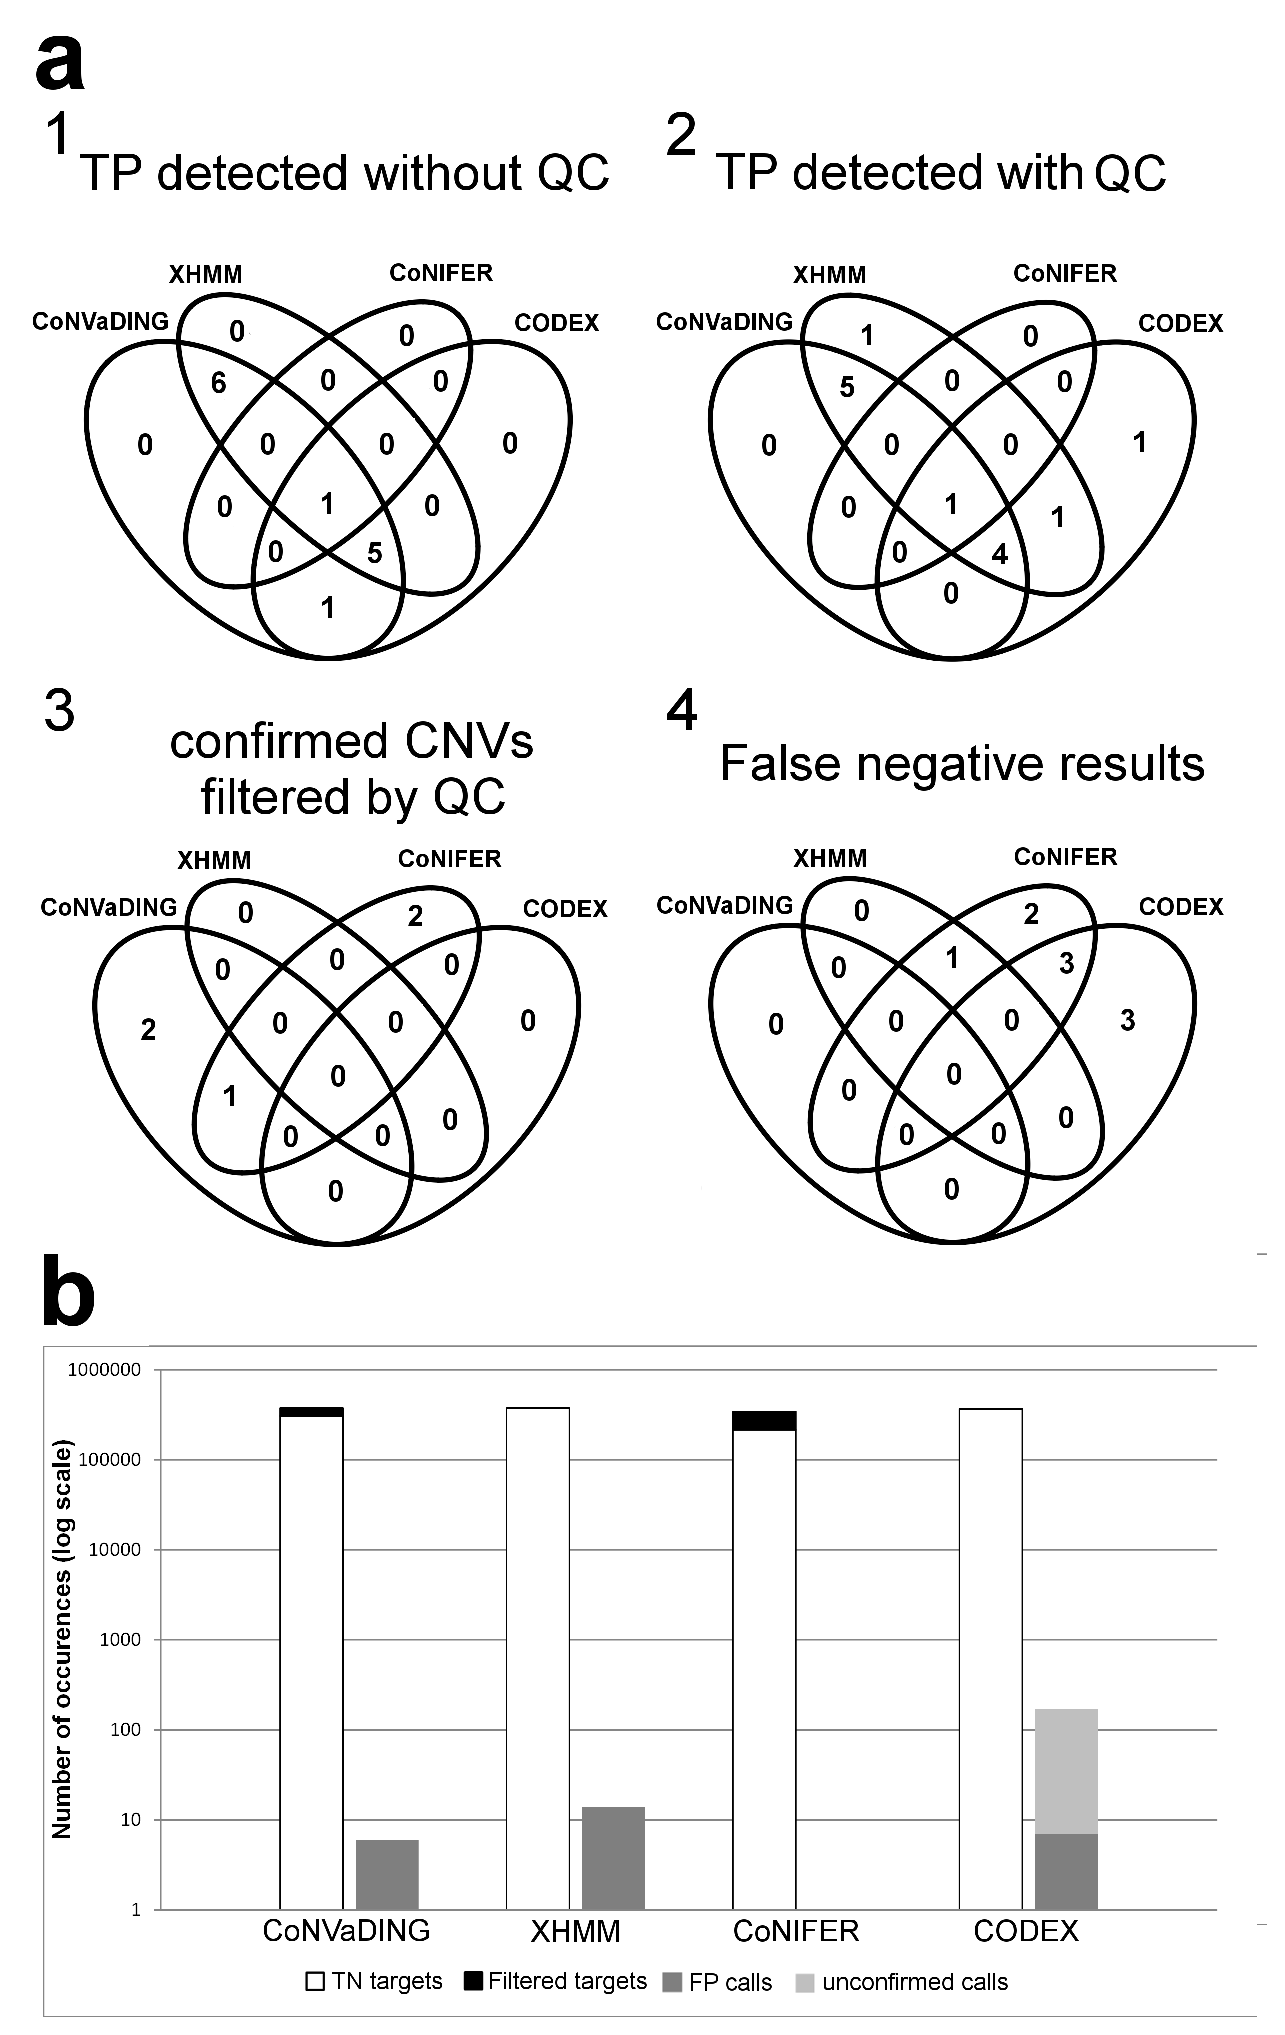
\includegraphics[width=0.9\linewidth]{img/CoNVaDING_Fig3}
	\caption[CNV detections CoNVaDING, XHMM, CoNIFER, and CODEX]{Caption next page.}
	\label{fig:CoNVaDING_Fig3}
\end{figure}
\addtocounter{figure}{-1}
\begin{figure}
	\caption[]{(Previous page.)CNV detections made by CoNVaDING, XHMM, CoNIFER, and CODEX. A: Venn diagrams showing true- positive (TP) and false-negative (FN) calls (1) TP detected without quality control (QC), (2) TP detected with QC, (3) confirmed CNVs filtered by QC, and (4) FN results. B: Bar plot using a log 10 scale showing the true-negative (TN), filtered targets (FT), false-positive (FP) results, and unconfirmed calls.}
\end{figure}

\subsection{Comparison to CoNIFER, XHMM and CODEX}
In the CoNIFER analysis, 42\% of samples failed to pass Sample QC: 31 and 102 for the FC and CM panels, respectively. 
In the remaining samples only one TP CNV (del 5 exons BRCA1) was identified and no additional CNVs were detected. 

In the XHMM analysis, all samples passed Sample QC and only three targets in the FC panel and five in the CM panel failed Target QC. 
Twelve TP and thirteen FP CNVs were called. 
Only one of the FP results, a one exon PLN duplication, was also detected by CoNVaDING. 
XHMM produced one FN result, since it did not detect the 1 exon MSH2 deletion, even though that sample and target had passed QC. 
In the CODEX analysis, all samples passed Sample QC and fourteen targets in the FC panel and thirty in the CM panel failed Target QC. 
In total, seven TP CNVs were called among 165 other calls, 49 in the FC, and 116 in the CM panel, respectively (Supplemental Table S4). 
Of those other calls, 112 calls were found in samples that failed CoNVaDING sample QC, 36 and 76 for the FC and CM panels, respectively. 
Due to the high number of novel calls, we did not confirm CNVs that were called only by CODEX. 
However, six calls were confirmed FP, because these were either called by XHMM or were present on the CoNVaDING shortlist. 
CoNIFER, XHMM, and CODEX analysis resulted in sensitivities of 16.7\%, 92.3\%, and 53.8\% and specificities of 100\%, 99.997\%, and 99.955\%–99.998\%, respectively, for targets passing all QC. 
Ten of the 13 FP findings by XHMM were located in samples or targets that failed CoNVaDING Sample QC or Target QC. 
Supplemental Table S3 shows all CNVs detected by one ormore of the tools. 
A comparison of FP and TN results is shown in Figure  \ref{fig:CoNVaDING_Fig1}B.



\subsection{Performance of CoNVaDING on Low-Coverage Data}
Using default settings, 101 FC and eight CM samples passed
sample QC at an average coverage of 100x and no sample passed sample QC at a coverage of 50x. 
To enable analysis, sample QC thresholds were increased to 0.11 and 0.13 for the 100x and 50x coverage samples, respectively. Using these settings, 117 FC and 179 CM samples passed sample QC at a coverage of 100x. 
These numberswere 112 and 31 for the FC and CM panels, respectively, at 50x coverage. 
At a coverage of 100x, only 60,663 (50\%) and 38,749 (15\%) of the targets analyzed passed all QC for the FC and CM panel, respectively. 
At a coverage of 50x, these numbers were 2,825 (2.3\%) and 1,014 (0.4\%). 
At 100x coverage, eight of the 13 CNVs that were confirmed by MLPA were detected and one remained at a coverage of 50x (Supplemental Table S5).
However, given a target passing both Target QC and Sample QC, the sensitivity stayed at 100\%. Specificity was 99.993\% (seven FP results) and 100\% at a coverage of 100x and 50x, respectively.


\section{Discussion}\label{discussion}
We have developed CoNVaDING, as a tool for detecting single exon CNVs in targeted NGS data. 
CNV detection in targeted NGS data is a challenge, because not every targeted region can be analyzed reliably. 
Therefore, for each target, CoNVaDING determines whether a high sensitivity and specificity can be obtained. 
This is especially important in a clinical diagnostic setting, where it is necessary to know exactly those targets for which a CNV could remain undetected.Adding information about failed targets indicates which targets should be tested using another method and for which targets a deletion or duplication can be detected or ruled out with high confidence. In our validation, we used high-coverage NGS data from targeted gene panels. 
By analyzing all potential CNVs using MLPA, we could validate calls as small as a single exon and accurately determine sensitivity and specificity. After MLPA, we determined a 100\% sensitivity and a 99.998\% specificity for CoNVaDING analysis in targets passing QC. 
Previous validations of XHMM and CoNIFER were based on concordance between SNP array calls and whole-exome sequencing data. 
The validation studies using this approach determined a sensitivity of 67\% for XHMM \cite{Fromer_2012} and 76\%–84\% for CoNIFER \cite{Krumm_2012}. 
In contrast, we found a higher sensitivity for XHMM calls (92.3\%) and much lower sensitivity (16.7\%) for CoNIFER. 
It may be that CoNIFER CNV calling was hampered by the small CNV size in our positive control samples. 
In the previous CODEX validation study, sensitivity was determined using a simulation data set and approached 100\% sensitivity for rare CNVs having a minimum length of five exons \cite{Jiang_2015}. 
In our study, we called three out of four CNVs having five exons or more (75\%) and four out of nine (44.4\%) CNVs smaller than five exons.

Our data show that CoNVaDING outperforms CoNIFER, XHMM, and CODEX because of its QC metrics, making high-coverage NGS gene panel data suitable as first line CNV detection data, regardless of the CNV size. 
CoNVaDING flagged around 10\% of the targets as low quality, indicating that these targets are not suitable for single exon variation detection due to a high variability of that target in the selected control samples. 
However, multiple exon variations containing low-quality targets can still be detected, as long as part of the CNV region is of sufficient quality. 
The moderate numbers of samples and targets flagged as low quality by CoNVaDING, combined with FP XHMM results in these samples and targets, suggest that CoNVaDING quality metrics successfully filter out samples and targets with a higher likelihood of FP results. 
The high number of excluded CoNIFER samples and the absence of failed samples and near absence of failed targets in XHMM and CODEX analysis suggest suboptimal QC performance of these tools. 
Our results also suggest that specificity can be even further improved by combining CoNVaDING with the other algorithms, since there is only a small overlap between FP calls and a high concordance in TP calls (Supplemental Table S3). 
CoNVaDING is primarily designed for detection of rare germline CNVs by targeted sequencing and for use in both research and clinical settings. 
The presence of (common) CNVs in the set of possible control samples may lead CoNVaDING to consider the targets within the CNV region as low quality. 
We determined the effect of a lower coverage on the performance of CoNVaDING. 
Since variability between samples increases at a lower coverage,more targetswere labeled as low quality. 
The number of targets passing QC was considerably higher in the FC than in the CM panel, suggesting that the minimum coverage needed differs per capturing panel. 
Given the results of the analysis of downsampled targets, we expect CoNVaDING to be able to analyze 15\%–50\% of the targets in a 100x coverage exome at a single-exon resolution. 
At a lower resolution, we expect more targets to pass QC. 
We also tested CoNVaDING on low-coverage whole-genome sequencing data (30x average) using 10 kb bins as targets. 
Although the increased bin size lowered the resolution as comparedwith analysis in high coverage data, a high concordance with SNP array data was found for calls larger than 50 kb. 
The extent to which this can be used as a method to detect smaller CNVs is currently being investigated. 
In conclusion, CoNVaDING improves sensitivity and specificity as well as QC for CNV analysis of NGS data. 
Our tool shows not only which CNVs are detected, but also which specific targets are unreliable for CNV analysis. 
We consider CoNVaDING uniquely fit for detection of single exon CNVs in targeted NGS data, making it an indispensable addition to the CNV detection tool box in both research and clinical diagnostic settings.


\section{Acknowledgments}\label{Acknowledgments} 
We thank Jackie Senior and Kate Mc Intyre for editorial advice.


\subsubsection{Disclosure Statement} 
The authors declare no conflict of interest.

\subsubsection{Supplemental Material}
Supplemental methods and tables: \\ https://onlinelibrary.wiley.com/doi/abs/10.1002/humu.22969 \\
\\
CoNVaDING source code and documentation: \\ https://github.com/molgenis/CoNVaDING  \\
\\
CoNVaDING video tutorial: \\ https://www.youtube.com/watch?v=-geFWkvKZzE\&feature=youtu.be
\chapter[Using a diagnostic gene panel for opportunistic screening]{What if we would use a diagnostic multi-cancer gene panel for opportunistic screening? A study in 2,090 Dutch familial cancer patients}
\chaptermark{opportunistic screening}
\label{chap:Opportunistic_screening}

{ \Large \leftwatermark{
		\put(-67,-66.5){ 1 }
		\put(-67,-91.5){ 2 }
		\put(-67,-116.5){ 3 }
		\put(-76.5,-150){
\includegraphics[scale=0.8]{img/thumbindex.eps}} \put(-67,-141.5){ {\color{white} 4 }}
		\put(-67,-166.5){ 5 }
		\put(-67,-191.5){ 6 }
		\put(-67,-216.5){ 7 }
		\put(-67,-241.5){ 8 }
		\put(-67,-266.5){ 9 }
		\put(-67,-291.5){ 10 }
		\put(-67,-316.5){ 11 }
	} \rightwatermark{
		\put(350.5,-66.5){ 1 }
		\put(350.5,-91.5){ 2 }
		\put(350.5,-116.5){ 3 }
		\put(346.5,-150){
\includegraphics[scale=0.8]{img/thumbindex.eps}} \put(350.5,-141.5){ {\color{white} 4 }}
		\put(350.5,-166.5){ 5 }
		\put(350.5,-191.5){ 6 }
		\put(350.5,-216.5){ 7 }
		\put(350.5,-241.5){ 8 }
		\put(350.5,-266.5){ 9 }
		\put(350.5,-291.5){ 10 }
		\put(350.5,-316.5){ 11 }
}}

\hfill \underline{submitted} 


\newpage

\noindent
L.F. Johansson\textsuperscript{1}, K.K. van Dijk-Bos\textsuperscript{1}, A.H. van der Hout\textsuperscript{1}, A.P. Knopperts\textsuperscript{1}, B. Leegte\textsuperscript{1}, P.C. van den Akker\textsuperscript{1}, K. Kok\textsuperscript{1}, I.M. van Langen\textsuperscript{1}, M.A. Swertz\textsuperscript{1}, R.K. Weersma\textsuperscript{2}, R.J. Sinke\textsuperscript{1}, B. Sikkema-Raddatz\textsuperscript{1}, H. Westers\textsuperscript{1,*}, R.H. Sijmons\textsuperscript{1,*}\\


\noindent
University of Groningen, University Medical Center Groningen, 1. Department of Genetics, 2. Department of Gastroenterology, Groningen, The Netherlands\\

\noindent* these authors contributed equally to the paper


\section*{Abstract}\label{abstract}
\subsubsection{Purpose}
In familial cancer (FC) diagnostics, analysis of next-generation sequencing data typically focuses on genes known to be associated with the cancer type that prompted referral. Currently, however, it is debated whether opportunistic screening should be performed when sequence data is available for other genes. We aimed to determine how many secondary findings (SFs) would be detected in cancer-predisposing genes present in our FC gene panel if we offered opportunistic screening to patients within FC diagnostics.
\subsubsection{Methods}
We anonymously reanalyzed sequencing data of 2,090 FC patients for either 73 genes (original FC panel) or 85 genes (updated panel) for SNVs, indels and CNVs. To determine the background prevalence of pathogenic variants in FC genes, we screened 1,326 individuals from the general Dutch population.
\subsubsection{Results}
We detected SFs in 3.0\% of patients (excluding heterozygous \textsl{CHEK2} and \textsl{MUTYH} variants), and a (likely) pathogenic variant matching their family’s cancer type in 10.1\% of patients. In the Dutch population cohort, 3.2\% of individuals had a (likely) pathogenic variant in a cancer-predisposing gene. 
\subsubsection{Conclusion}
Our results can assist in the design of future research programs on opportunistic screening. These programs are needed because there is not yet sufficient evidence to meet international screening program criteria. 

\section{Introduction}\label{introduction}
Next-generation sequencing (NGS) allows for simultaneous diagnostic testing of many genes, and NGS gene panels are now commonly used in familial cancer (FC) diagnostics \cite{Okur_2017}. 
These panels typically target particular tumor types or a combination of them (e.g. colorectal cancer or breast and ovarian cancer). 
This approach deliberately limits the chance of detecting pathogenic variants in genes associated with cancer types other than the tumor types that triggered referral, i.e. secondary findings (SFs) \cite{DeRycke_2017,Concolino_2018}. 
Diagnostic panels could, however, be used for other purposes. 
Firstly, the systematic use in FC diagnostics of broader gene panels, including new candidate cancer-predisposing genes, could help define the phenotypes associated with variants in newly postulated genes. 
This might, in time, increase the molecular diagnostic yield in patients referred for FC, as $\sim$90\% of these patients are currently left without a molecular diagnosis \cite{Tung_2016,Thompson_2016,Minion_2015,LaDuca_2014}. 
Secondly, extended panels would allow for opportunistic screening for actionable variants in a broader range of cancer-predisposing genes, rather than limiting their use to the genes associated with the cancer type(s) that prompted referral. The pros and cons of opportunistic genetic screening and reporting SFs in patients who undergo diagnostic testing are currently the subject of a debate triggered by statements by the American College of Medical Genetics and Genomics (ACMG) that advocate such screening and reporting \cite{Green_2013,Burke_2013,Yu_2014,Kalia_2016,Haer_Wigman_2018,Wouters_2018,Brothers_2019,Esplin_2018}. 
Performing this kind of screening in addition to diagnostics is not part of current Dutch clinical genetics services because it would be regarded as population screening, which is not allowed without special permission by Dutch authorities. However, screening could be of health benefit to our patients, and therefore further discussion is thus warranted in the context of a clinical genetics service system that is already under pressure by increasing numbers of referrals. 
As part of this discussion, it is important to establish the scope and frequency of SFs we expect to see if broad diagnostic cancer gene panels are used for screening. 

We developed an 85-gene, multi-cancer targeted NGS gene panel and implemented it in our genome diagnostics laboratory. 
For diagnostic purposes clinicians in our center can request analysis of only particular subsets of genes in the panel that are known to be related to the tumor types in families. 
For research purposes, all panel genes, including newly postulated tumor syndrome genes, are analyzed anonymously for all patients.

The primary aim of this study was to estimate the number of SFs that we would detect if, in addition to diagnostic testing, we were to screen for variants in genes beyond those with known associations to the referral cancer type. 
We sought to estimate this number against the background of diagnostic yield of our gene panel in a cohort of 2,090 patients referred to our clinic for FC diagnostics, a process that included the testing for single nucleotide variants (SNV), indel variants and copy number variants (CNV). 
In the near future opportunistic screening for cancer-related variants, and others that are outside the scope of our paper, could be made available to more patients as exome testing becomes more prevalent for many types of conditions. 
To estimate the number of SFs in case of opportunistic screening in Dutch patients, in general, we also analyzed SNVs, indels and CNVs in the 85 panel genes in the dataset of all 498 non-related individuals from the Dutch genome sequencing project Genome of the Netherlands (GoNL) \cite{Francioli_2014} and in exome data of 828 samples from the LifeLines Deep (LLD) consortium, which is representative of the population in the northern Netherlands \cite{Tigchelaar_2015}.
Another reason for the population study was that if we would find significantly more SFs in our FC cohort than expected given general population frequencies, this would suggest that some of the SFs might actually be diagnostic, reflecting expanded tumor syndrome phenotypes.

Across these analyses, we determined which variants would be eligible for return based on two sets of guidelines that list genes eligible for return of SFs: one recommended by the ACMG and one from the French Society of Predictive and Personalized Medicine (SFMPP). 
Based on our results, we assessed if such screening meets proposed genetic screening criteria \cite{Andermann_2008}. 
Hereby we aim to add context to the discussion if, or which, variants should be returned to an individual in absence of a reason for diagnostic testing for those variants. 

\section{Materials and Methods}\label{methods}
\subsection{Patient cohorts}
This study was performed in accordance with Dutch and University Medical Center Groningen (UMCG) ethical guidelines. 
All patients involved had been referred to the FC Clinic of the department of Genetics of the UMCG for genetic diagnostics and counseling. 
Patients were seen between March 2013 and January 2017. Referrals for testing met the Dutch guidelines for genetic testing \cite{Erfelijk_2010}. 
For molecular diagnostic purposes, only those genes from the NGS panel that were in the differential diagnosis for the patient and family tumor type, were analyzed. 
The outcomes of these “virtual” subpanels extracted from the full dataset were reported to the genetic counselor and discussed with the patient and referring physician. 
For the purpose of our research, the sequencing data of all panel genes were analyzed anonymously in all patients. 
Personal and family histories regarding tumors (including intestinal polyps) were available. 

Our patient population for FC panel testing consisted of two cohorts: \newline
\noindent\textbf{Cohort A (n=198)} is a ‘retrospective cohort’ of patients who previously tested negative, using Sanger sequencing, for selected genes that seemed most appropriate given their cancer type (e.g. \textsl{BRCA1/2} in breast cancer patients). 
These patients were sequenced using the NGS panel in 2013 and 2014 and were selected based on having the pedigrees most suspect for a genetic predisposition: their age at cancer diagnosis was at least 5 years younger than the minimum age in the referral guidelines and/or they had more than the minimum number of affected relatives required for referral. 
We included this cohort because it reflects our clinical practice of re-analyzing unsolved families, especially the more suspect ones, with new techniques.
\newline
\noindent\textbf{Cohort B (n=1,892)} is a ‘prospective cohort’ of patients referred to our clinical genetics department between 2014 and 2017 for FC diagnostics. 
Subpanel testing was the first genetic diagnostic test performed in these patients. 

\subsection{General Dutch population cohort}
We used data from two general Dutch population cohorts to determine the population frequency of variants in the genes in our targeted panel. 
The first cohort is a representative subset of the Dutch population produced by the GoNL project, from which we included 498 non-related individuals \cite{Francioli_2014}. 
The second cohort consists of 828 participants of the LLD cohort \cite{Tigchelaar_2015}. 
Possible cancer phenotypes of GoNL or LLD participants were unknown to the researchers and cannot be excluded. Further details are available in the supplementary methods.

\subsection{Selection of genes for the NGS panel}
In March 2013, as part of our clinical FC diagnostics service in the UMCG, we developed and validated an NGS panel that contained 73 tumor syndrome genes (SureSelectXT Custom design \#0421101, referred to as \textbf{panel 1} here) (Agilent Technologies, Santa Clara, CA). 
The design and validation methods for this panel have been reported previously \cite{Sikkema_Raddatz_2013}. 
In June 2015, the panel was updated with the addition of 13 genes and the removal of one gene, resulting in an 85-gene panel (SureSelectXT Custom design \#0735701, referred to as \textbf{panel 2} here) (table \ref{table:screening_table1}).
The Fanconi anemia genes (other than \textsl{BRCA2} and \textsl{PALB2}) were left out of the panel as these were included in a separate hematology panel (not tested in our study). 

\begin{table}
\caption[Panel 1 and 2 genes and ACMG and SFMPP inclusion]{Genes present on panels 1 and 2 and their inclusion on the ACMG and SFMPP lists for recommended return.}
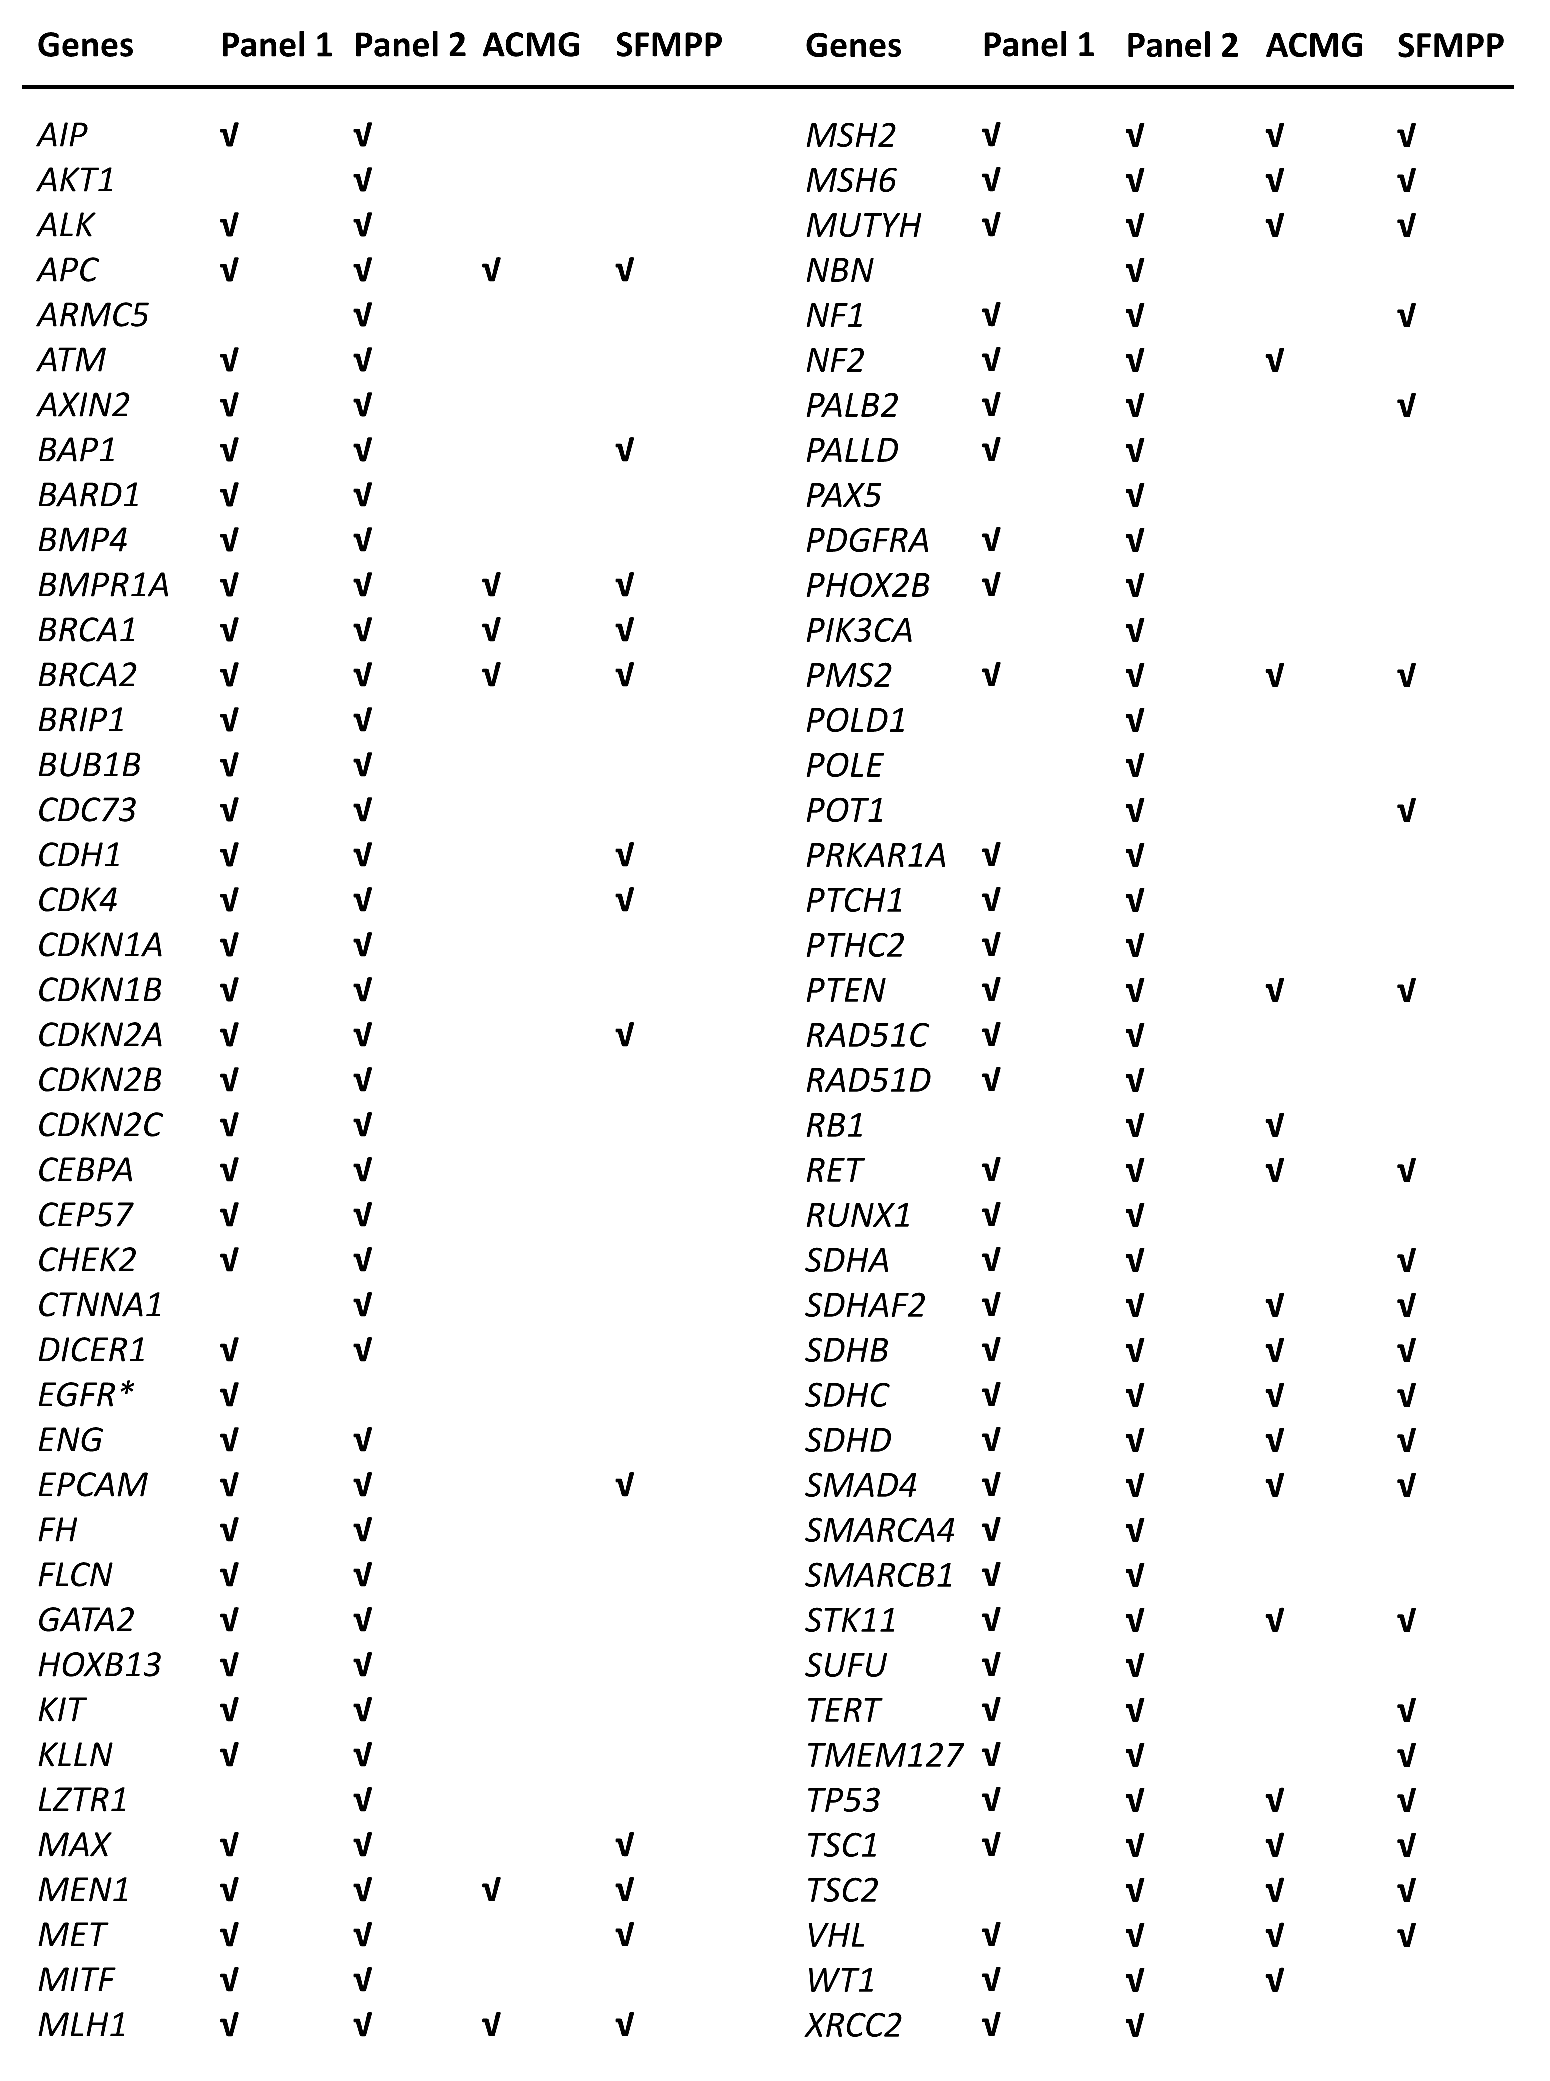
\includegraphics[width=1.0\linewidth]{img/opportunistic_screening_Table1}
 \caption*{\footnotesize{*not included in analysis}}
\label{table:screening_table1}
\end{table}

\subsection{Sequencing and alignment procedure}
All samples were prepared and sequenced according to the SureSelectXT Automated Target Enrichment for Illumina Paired-End Multiplexed Sequencing protocol (Agilent Technologies). 
In short, high molecular DNA was isolated from peripheral blood lymphocytes and randomly fragmented, followed by end repair, dA tailing and adapter ligation. 
Regions of interest were captured using a biotinylated cRNA probe solution (Agilent Technologies) using one of the two panels. Subsequently 151 bp paired-end sequencing was performed on an Illumina Miseq. 
Reads were aligned using Burrows-Wheeler Aligner (BWA) v0.7.12 \cite{Li_2010}. 
SNVs and indels were called using GATK HaplotypeCaller v3.5 and CNVs using CoNVaDING \cite{Johansson_2016b} and XHMM \cite{Fromer_2012}. 
Complete procedures are described in the supplementary methods. 
CNV calls of more than two exons that were made by both tools in samples that passed both CoNVaDING and XHMM sample quality control (QC) metrics were considered reliable and were not tested using another technique. 
All other calls were confirmed using either the Illumina HumanCytoSNP-850K-8 v1.1 array (Illumina, San Diego, CA) or the Multiplex Ligation-dependent Probe Amplification (MRC-Holland, Amsterdam, the Netherlands) using the manufacturer’s protocols. 

\subsection{Data analysis and interpretation}
The 198 patients in Cohort A (negative previous single gene analysis) and 299 patients from Cohort B were analyzed with gene panel 1. 
They were also screened for the \textsl{POLE} c.1270C$\textgreater$G (p.L424V) and \textsl{POLD1} c.1433G$\textgreater$A (p.S478N) hotspot variants \cite{Palles_2012} using Sanger sequencing (as explained in the supplementary methods). 
The remaining 1,593 patients were analyzed using panel 2. 
For the general Dutch population samples only variants in our 85 panel genes were interpreted. 
No CNV detection was performed in the LLD samples.

The variant analysis we use in the UMCG clinical genetics department is based on the ACMG rules \cite{Richards_2015}. 
All annotated variants were analyzed using Cartagenia software (Agilent Technologies Bench Lab NGS v4.3.5) and Alamut (Alamut version 2.4, Interactive Biosoftware, Rouen, France). 
Variants were labeled in five classes (benign, likely benign, variant of unknown clinical significance (VUS), likely pathogenic and pathogenic) following the proposal of Plon et al \cite{Plon_2008}, with VUS equaling class III.

Variants were considered to add to the molecular diagnostic yield if they were labeled as pathogenic or likely pathogenic and found in a gene with an established relationship to (at least one of) the referral cancer type(s). This included both highly penetrant and more moderately penetrant variants (e.g. in \textsl{CHEK2}). 
\textsl{MUTYH} variants were only included if they were homozygous or compound heterozygous. 
Variants were considered SFs when they were labeled (likely) pathogenic and had no established relation to any of the referral cancer types. 
Some SFs may actually turn out to represent extended phenotypes associated with the genes in question and thus go on to become primary findings. 
Some of these extensions have already been suggested, but not yet proven, in the literature. We therefore labelled SFs for which extended phenotypes have been suggested to match the patient’s referral cancer type as ‘suggested’. 
Variants in our analysis are thus labelled as having established, suggested or no relation with the referral cancer type(s). 
To determine how many actionable SFs would be found, (likely) pathogenic variants in the population cohorts were further filtered based upon two lists of genes in which (likely) pathogenic variants are considered to be actionable and recommended for return: the ACMG SF v2.0 list \cite{Kalia_2016}, which contains 25 cancer-related genes, all present in our panel, and 36 cancer-related genes from the SFMPP list \cite{Pujol_2018}, of which 35 are present in our panel (table \ref{table:screening_table1}).

All the variants detected in our study have been submitted to the public locus-specific databases of the Leiden Open Variant Database platform (www.lovd.nl/3.0/home). 

\section{Results}
\subsection{Sequencing quality}
For all samples, NGS quality met the criteria used in our genome diagnostic laboratory ($\textgreater$80\% of the bases were sequenced with a quality $\ge$Q30). 
After alignment and duplicate removal, the average coverage for targeted regions was 423$\times$ (sd 161$\times$) and 447$\times$ (sd 307$\times$) for panels 1 and 2, respectively, and \textgreater98\% of targeted bases were covered by at least 20 reads. 
Of the samples, 197 (99.5\%) retrospective cohort samples and 1,520 (95.4\%) prospective cohort samples passed CoNVaDING sample QC and were suitable for single exon CNV detection.     

\begin{table}
	\caption[Number of pathogenic variants found per referral cancer type]{\textbf{Number of pathogenic and likely pathogenic variants found per referral cancer type}}
	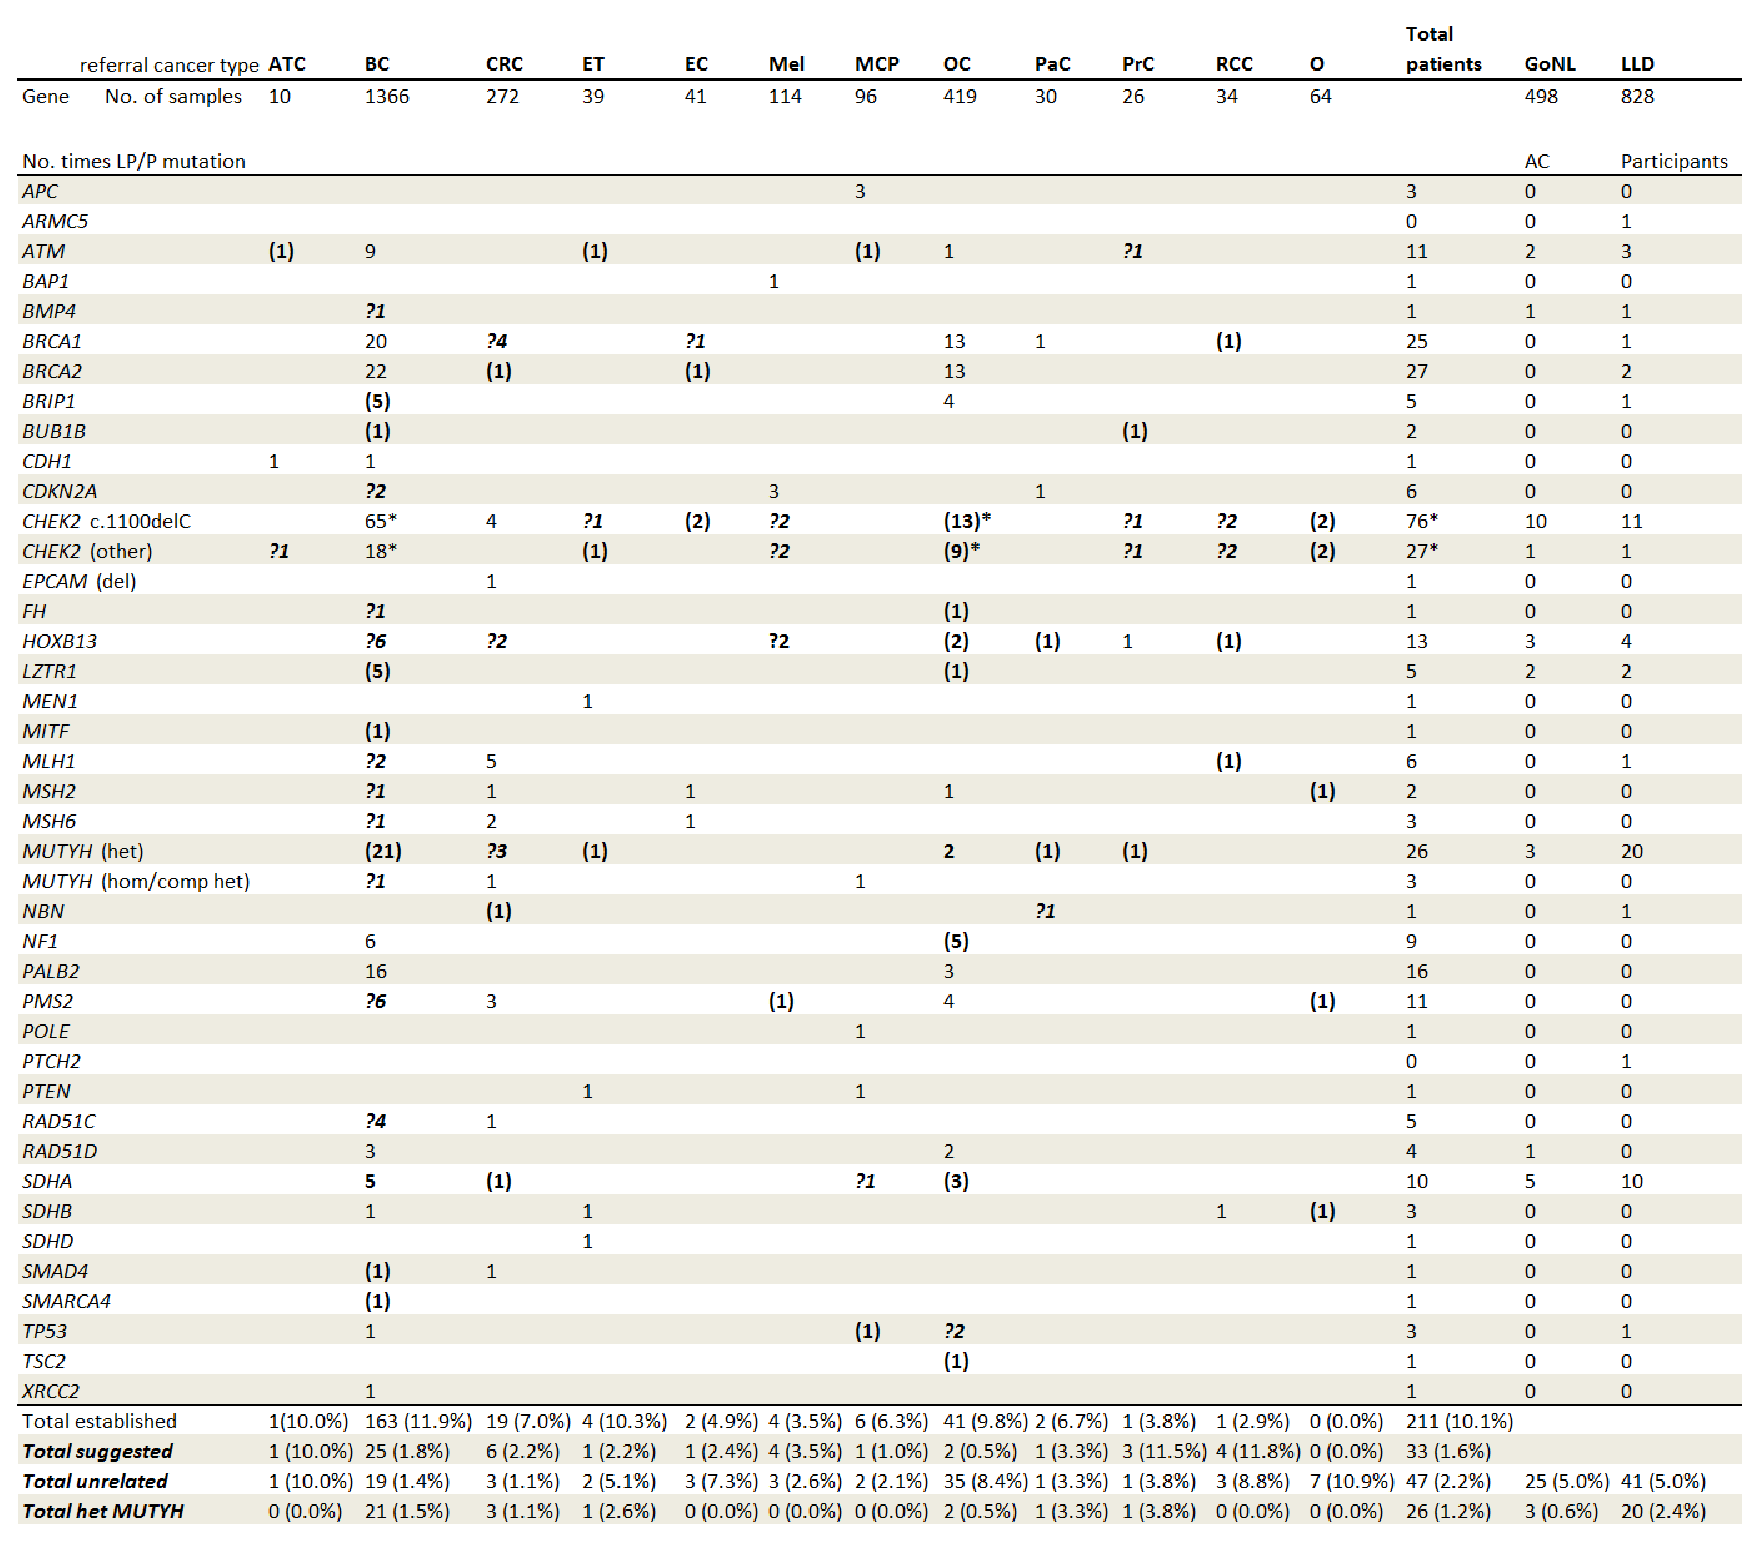
\includegraphics[width=1.0\linewidth]{img/opportunistic_screening_Table2}  %%Font does not support bold italic text.
		\caption*{\footnotesize{Plain text = gene with established relation to cancer phenotype; \textbf{Bold} text = secondary finding, encompassing: \textbf{Bold ()} = Gene with no relation to cancer phenotype; \begin{bfseries}\textit{Bold Italics ?}\end{bfseries} = Gene with suggested relation to cancer phenotype, *One sample homozygous or compound heterozygous, **All three positive instances have gastric cancer as the referral cancer type, ***Various endocrine tumor types (\textsl{ATM} and \textsl{CHEK2} other: neuroendocrine tumor; \textsl{CHEK2} c.1100delC, \textsl{MUTYH} het, \textsl{PTEN} and \textsl{SDHB}: Thyroid cancer; \textsl{MEN1}: Parathyroid adenoma; \textsl{SDHD}: Paraganglioma). ATC: alimentary tract cancer; BC: breast cancer; CRC: colorectal cancer; ET: endocrine tumor; EC: endometrial cancer; Mel: melanoma; MCP: multiple colorectal polyps; OC: ovarian cancer; PaC: pancreatic cancer; PrC: prostate cancer; RCC: renal cell cancer; O: Other cancer types; GoNL: Genome of the Netherlands cohort; LLD: Lifelines Deep cohort; AC: Allele count; het: heterozygous; hom: homozygous; ch: compound heterozygous. Genes without any likely pathogenic or pathogenic variant in any of the cohorts: \textsl{AIP}, \textsl{AKT1}, \textsl{ALK}, \textsl{AXIN2}, \textsl{BARD1}, \textsl{BMPR1A}, \textsl{CDC73}, \textsl{CDK4}, \textsl{CDKN1A}, \textsl{CDKN1B}, \textsl{CDKN2B}, \textsl{CDKN2C}, \textsl{CEBPA}, \textsl{CEP57}, \textsl{CTNNA1}, \textsl{DICER1}, \textsl{ENG}, \textsl{FLCN}, \textsl{GATA2}, \textsl{KIT}, \textsl{KLLN}, \textsl{MAX}, \textsl{MET}, \textsl{NF2}, \textsl{PALLD}, \textsl{PAX5}, \textsl{PDGFRA}, \textsl{PHOX2B}, \textsl{PIK3CA}, \textsl{POLD1}, \textsl{POT1}, \textsl{PRKAR1A}, \textsl{PTCH1}, \textsl{RB1}, \textsl{RET}, \textsl{RUNX1}, \textsl{SDHAF2}, \textsl{SDHC}, \textsl{SMARCB1}, \textsl{STK11}, \textsl{SUFU}, \textsl{TERT}, \textsl{TMEM127}, \textsl{TSC1}, \textsl{VHL}, \textsl{WT1}.}
	}
	\label{table:screening_table2}
\end{table}

\subsection[Patient cohort: variant analysis]{Patient cohort: variant analysis for diagnostic yield and secondary findings}
In the combined cohorts of 2,090 patients, we detected 324 pathogenic or likely pathogenic variants (SNV, indel and CNV) in 302 (14.4\%) patients distributed over 37 of the genes included in the panel, including two homozygous and three compound heterozygous variants (Table \ref{table:screening_table2} and Supplementary table 1). %%INSERT TABLE
In 48 genes no (likely) pathogenic variants were found.

In the retrospective cohort (n=198) we found 18 (likely) pathogenic variants in 16 patients (8.1\%). 
None of these were CNVs. 
Of the 18 (likely) pathogenic variants, 14 (7.1\%) had an established relation to at least one of the phenotypes warranting referral (Table \ref{table:screening_table3} \& Supplementary table 2). 
The remaining four variants (2.0\%) were classified as SF. 
Two of these patients also had a pathogenic variant with an established relation to the referral cancer type (Table \ref{table:screening_table3} \& Supplementary table 3). 
Of the four SFs one was suggested to be related to the referral cancer type. 
Further research may confirm or disprove this suggestion. None of the four SFs were on the ACMG or SFMPP lists for recommended return. 
In addition, three heterozygous \textsl{MUTYH} pathogenic variants were found (Table \ref{table:screening_table3} \& Supplementary table 4). %insert table
A total of 54 VUSs were found (27.3\%), including four CNVs. 

\begin{table}
	\caption[Genes with pathogenic and likely pathogenic variants]{\textbf{Genes with pathogenic and likely pathogenic variants}}
	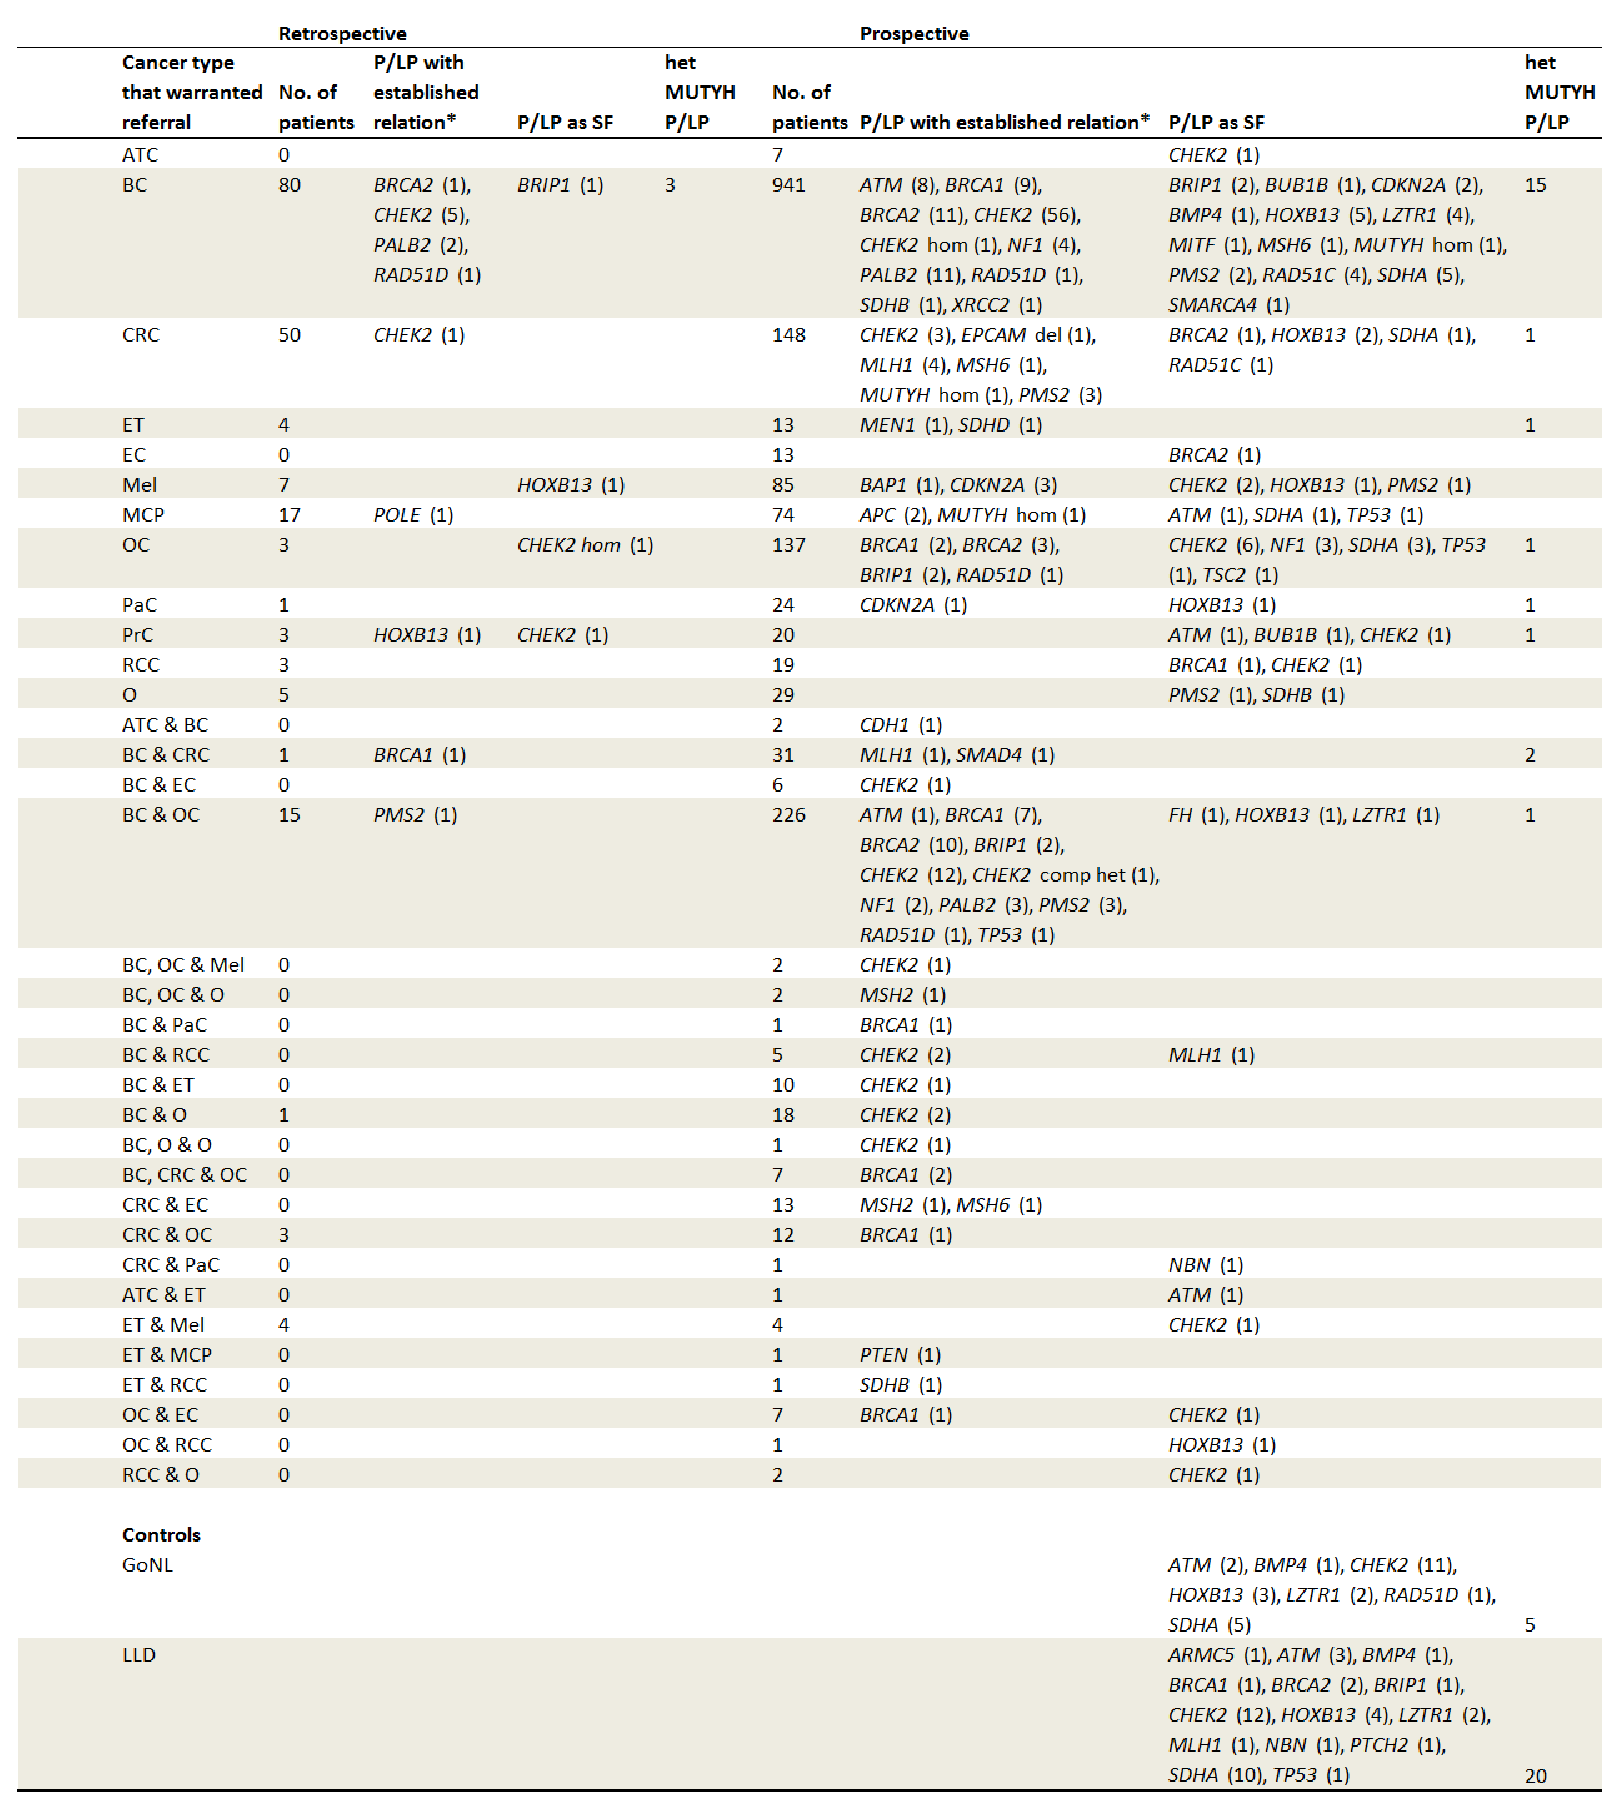
\includegraphics[width=1.0\linewidth]{img/opportunistic_screening_Table3}
		\caption*{\footnotesize{\textsl{Gene} (number of times (likely) pathogenic variant in gene); ATC: alimentary tract cancer; BC: breast cancer; CRC: colorectal cancer; ET: endocrine tumor; EC: endometrial cancer; Mel: melanoma; MCP: multiple colorectal polyps; OC: ovarian cancer; PaC: pancreatic cancer; PrC: prostate cancer; RCC: renal cell cancer; O: Other cancer types; GoNL: Genome of the Netherlands cohort; LLD: Lifelines Deep cohort. *to at least one of the cancer phenotypes}}
	\label{table:screening_table3}
\end{table}


In the prospective cohort (n=1,892), in 197 patients (10.4\%), we found a (likely) pathogenic variant in a gene that could explain or might have contributed to the family’s cancer type and that matched the patient’s reason for referral (Figure \ref{fig:screening_Fig1}, Table \ref{table:screening_table3} \& Supplementary table 2). %insert table and figure
Of these patients, two carried two independent (likely) pathogenic variants that matched their cancer type(s), and four carried a compound heterozygous or homozygous variant (2$\times$  \textsl{CHEK2} and 2$\times$  \textsl{MUTYH}). 
We excluded 23 heterozygous \textsl{MUTYH} variants (Table \ref{table:screening_table3} \& Supplementary table 4). %Insert table
Of the 201 (likely) pathogenic variants, 13 were CNVs. In addition, SFs were detected in 74 patients (3.9\%). 
Of these patients, two had two different SFs and eight had a second (likely) pathogenic variant with an established relation to the referral cancer type (Table \ref{table:screening_table3} \& Supplementary table 3). 
Of these 76 SFs, 32 have been suggested in the literature to be related to the referral cancer type. 
Further research may confirm or disprove these suggestions. The remaining 44 SFs had no established or suggested relation to any of the referral cancer types (2.3\% of patients when including heterozygous \textsl{CHEK2} variants and 2.0\% when excluding them). 

Of the 80 SFs found in the combined cohorts, including six CNVs, 14 (0.7\% of patients) would have been reported following ACMG recommendations (\textsl{MLH1}, \textsl{MSH2}, \textsl{BRCA1}, \textsl{BRCA2}, \textsl{MUTYH}, \textsl{PMS2}, \textsl{SDHB}, \textsl{TP53} and \textsl{TSC2}). 
When following the SFMPP list, an additional 15 SFs would have been reported (\textsl{CDKNA2}, \textsl{NF1} and \textsl{SDHA}), leading to a total of 1.4\% of patients. 
For the 80 SFs we found, 17 (21.3\% of SFs / 0.8\% of patients) have an established relation with other cancer types in the patient or family that were insufficient reason for genetic testing. 
In addition, 592 VUS were found, including 11 CNVs, in 492 patients in the prospective cohort.


\begin{figure}
	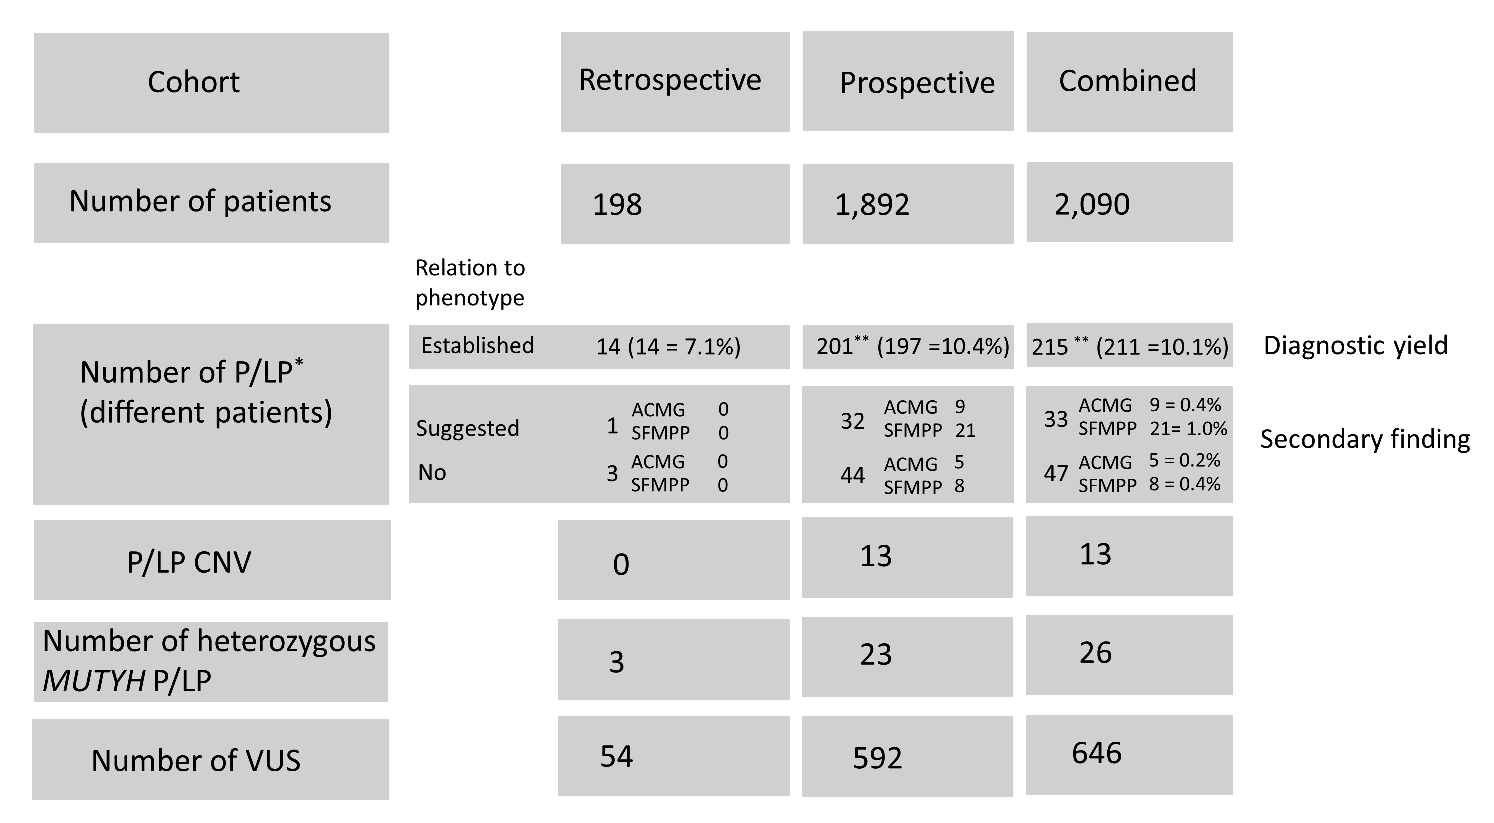
\includegraphics[width=1.0\linewidth]{img/opportunistic_screening_Fig1}
	\caption[Number of detected variants in the cohorts]{\textbf{Number of detected variants in the retrospective and prospective cohorts with their relation to the referral cancer type.} \footnotesize{*excluding heterozygous \textsl{MUTYH} variants. **compound heterozygous and homozygous variants both counted.}
	}
	\label{fig:screening_Fig1}
\end{figure}


The diagnostic yield percentages and SFs did not differ significantly between the retrospective and prospective cohorts (p-values Fisher’s Exact test (FET) \textgreater0.05).

\subsection{Control cohorts variant analysis}
To determine the expected yield of opportunistic screening in cancer-predisposing genes in patients referred for conditions other than FC we searched for (likely) pathogenic variants in the genes targeted by panel 2 in two control cohorts. 
In our cross-sectional Dutch population cohort of 498 individuals from the GoNL genome sequencing study, 14 (2.8\% when assuming a maximum of one pathogenic variant per individual) (likely) pathogenic variants were found in these genes (\textsl{ATM} 2$\times$, \textsl{BMP4}, \textsl{HOXB13} 3$\times$, \textsl{LZTR1} 2$\times$, \textsl{RAD51D}, \textsl{SDHA} 5$\times$), without including 11 (2.2\%) \textsl{CHEK2} and three (0.6\%) \textsl{MUTYH} variants (Table \ref{table:screening_table3} \& Supplementary table 5). %%INSERT TABLE
In addition, 106 VUS were found. Three of the \textsl{SDHA} variants concerned the same deletion of exons 6 and 7. 
None of the (likely) pathogenic variants were in genes present on the ACMG list for recommended return, while the five (1.0\%) \textsl{SDHA} variants are suggested to be reported by the SFMPP guidelines.

In the exome sequencing data of the 828 individuals from the LLD cohort, 29 (3.5\%) (likely) pathogenic variants were found in the genes targeted by panel 2 (\textsl{ARMC5}, \textsl{ATM} 3$\times$, \textsl{BMP4}, \textsl{BRCA1}, \textsl{BRCA2} 2$\times$, \textsl{BRIP1}, \textsl{HOXB13} 4$\times$, \textsl{LZTR1} 2$\times$, \textsl{MLH1}, \textsl{NBN}, \textsl{PTCH2}, \textsl{SDHA} 10$\times$, \textsl{TP53}), excluding 12 (1.5\%) heterozygous \textsl{CHEK2} and 20 (2.4\%) heterozygous \textsl{MUTYH} variants (Table \ref{table:screening_table3} \& Supplementary table 6).  %%INSERT TABLE
In addition, 172 VUS were found. Five of the pathogenic variants (0.6\%) are in genes present on the ACMG list for recommended return (\textsl{BRCA1}, \textsl{BRCA2}, \textsl{MLH1} and \textsl{TP53}), while the SFMPP list adds 10 (1.2\%) \textsl{SDHA} variants for recommended return.

\subsection{Comparison patient and control cohorts}
To determine a possible excess in SFs in our patient cohorts, which would indicate the presence of possible extended phenotypes, we compared the patient cohorts to the control cohorts. 
We assumed that all (likely) pathogenic variants in the control cohorts were present in different individuals. When excluding the heterozygous \textsl{CHEK2} and \textsl{MUTYH} variants and assuming variants in these genes are all heterozygous in the GoNL cohort, there is no significant difference in the number of patients with a SF versus the number of individuals in the control cohorts with a (likely) pathogenic variant (3.0\% (63/2,090) vs 3.2\% (43/1,326); FET p-value 0.7615). 
The same holds for the percentages of variants in genes suggested to be reported by the ACMG (0.7\% (14/2,090) vs 0.4\% (5/1,326); FET p-value 0.3472) or by the SFMPP (1.4\% (29/2,090) vs 1.5\% (20/1,326); FET p-value 0.7697).

\section{Discussion}
\subsection{Diagnostic yield}
In the patient cohort, SFs were detected against a background diagnostic yield of 10.1\% (211/2,090). 
This yield is in line with earlier reports, although it differs slightly depending on cancer type \cite{Hu_2018,Susswein_2015,Yurgelun_2017}. 
Detection of CNVs in our combined patient cohorts increased the diagnostic yield from 9.5\% to 10.1\%, providing an additional 13 patients with a molecular diagnosis. 
Of all (likely) pathogenic variants, 13 (6.1\%) were deletions of one or more exons, including the known Dutch founder mutations \textsl{BRCA1} deletion exon 22 and \textsl{SDHB} deletion exon 3 \cite{Petrij_Bosch_1997,Bayley_2009}. 
Given that a considerable fraction of the total yield comprised a CNV, and this information is readily available in the data, we recommend including CNV analysis in panel testing. 

\subsection[Secondary findings in families vs general population]{Secondary findings in referred families versus general population frequencies}
Our primary goal was to estimate the number of (likely) pathogenic variants we would find if we screened panel genes other than those with an established relation to the referral cancer type. 
If this opportunistic screening would have been offered to all patients, such a variant would have been identified in 63/2,090 patients (3.0\%), excluding heterozygous \textsl{CHEK2} and \textsl{MUTYH} variants, but including a homozygous \textsl{CHEK2} c.1100delC and a homozygous \textsl{MUTYH} c.91delG variant. 
Note that, in absence of a close relative with breast cancer, heterozygous \textsl{CHEK2} variants are not considered clinically actionable by Dutch guidelines (www.oncoline.nl). 
A heterozygous pathogenic \textsl{CHEK2} or \textsl{MUTYH} variant was detected as an SF in an extra 15 and 26 patients (0.7\% and 1.2\%), respectively. 
Of the 63 patients with an SF, eight also carry a variant matching their cancer type. In two patients, two separate SFs were detected. 
Views differ on what constitutes sufficient proof for actionability and on what to screen for and report. 
Limiting SFs to genes listed by the ACMG and SFMPP as targets for screening and reporting 14 (0.7\%) and 29 (1.4\%) actionable SFs would have been reported, respectively. 

Some SFs may turn out not to be secondary after all, but rather to be associated with as yet unknown expanded tumor syndrome phenotypes. 
Indeed, numerous publications suggests gene-tumor type associations outside the established tumor syndrome phenotypes, although, without providing definite proof. 
In our analysis such gene-tumor type combinations were labeled as ‘suggested’. 
Should all of these ‘suggested’ associations be confirmed in the future, which we suspect is unlikely, 26 extra diagnoses matching the referral phenotype would be made in our cohorts, which would increase diagnostic yield to 11.4\%. 

For a Dutch cohort of healthy parents of children with a \textsl{de novo} variant that caused intellectual disability, it was recently shown that 0.7\% (11/1,640) of people carried a dominant (likely) pathogenic oncogenetic variant in a gene present on the ACMG list, with an extra 1.9\% being a carrier of a heterozygous \textsl{MUTYH} variant \cite{Haer_Wigman_2018}. 
Here we expand our knowledge on the Dutch population frequency of (likely) pathogenic tumor syndrome gene variants by analyzing them in two independent cohorts. 
In the combined Dutch GoNL and LLD populations, the percentage of individuals with a (likely) pathogenic variant in the genes included in our NGS panel is 3.2\% (43/1,326), excluding the heterozygous \textsl{CHEK2} and \textsl{MUTYH} variants each present in 1.7\% (23/1,326) of samples. 
In the combined control cohorts 0.4\% (5/1,326), which does not differ significantly from the other Dutch parents cohort (FET p-value 0.3222), and 1.5\% (20/1,326) of individuals carried a (likely) pathogenic variant considered to be actionable according to the ACMG and SFMPP lists, respectively. Similarly, two other, non-Dutch, studies found an SF in an ACMG-listed cancer-predisposition gene in 0.4\% of individuals: a US-based patient study (25/6,240) \cite{Hart_2018} and a 1000 genomes cohort study (4/1,092) \cite{Olfson_2015}.  

In our three cohorts, five pathogenic variants were observed in relatively high percentages: \textsl{MUTYH} c.536A$\textgreater$G and c.1187G$\textgreater$A, \textsl{HOXB13} c.251G$\textgreater$A, \textsl{CHEK2} c.1100delC and \textsl{SDHA} c.91C$\textgreater$T. 
This was expected, given their known high prevalence in Western European populations \cite{Aretz_2013,Apostolou_2017,Liu_2016b,Oudijk_2012}. 


\begin{sidewaystable}
	\footnotesize
	\caption[Screening for secondary findings against screening criteria]{\label{table:summary}\textbf{Screening for cancer-predisposing gene variants as secondary findings in genetics diagnostics patients against screening criteria}}
	\begin{tabular}{ p{0.5cm} p{5.5cm} p{2cm} p{7cm} }
		 & \footnotesize{\textbf{Criterion}} & \footnotesize{\textbf{Criterion met}} & \footnotesize{\textbf{Comments}} \\
		\hline
		\multicolumn{4}{l}{\textbf{Classical Wilson and Jungner criteria (1-10) for screening programs \cite{Andermann_2008}}} \\
		\hline
		1 & The condition sought should be an important health problem & +/- & Cancer is an important health problem for patients. However, population frequency of cancer predisposing gene variants in absence of family history for the associated tumor types is relatively low. \\
		2 & There should be an accepted treatment for patients with recognized disease & +/- & For some disorders treatment is available, but for other disorders, this remains a challenge, e.g. screen-detected pancreatic lesions in pathogenic \textsl{CDKN2A} variant carriers. Consensus mainly exists for genes and their syndromes which are considered actionable of ACMG and/or SFMPP. \\
		3 & Facilities for diagnosis and treatment should be available & ? & Depending on your local, regional, national resources. In the Netherlands these are available \\
		4 & There should be a recognizable latent or early symptomatic stage & +/- & Dependent on type of cancer \\
		5 & There should be a suitable test or examination& + & Genetic variants can be reliably detected through sequencing \\
		6 & The test should be acceptable to the population & + & DNA sequencing is acceptable to patients tested for diagnostic reasons \\
		7 & The natural history of the condition, including development from latent to declared disease, should be adequately understood & +/- & True for the more common syndromes. For rare conditions/syndromes data are incomplete \\
		\hline
	\end{tabular}
	\caption*{ACMG = American College of Medical Genetics and Genomics; SFMPP = French Society of Predictive and Personalized Medicine; + criterion met; +/- criterion partly met; - criterion not met; ? uncertain if criterion is met.}
\end{sidewaystable}

\begin{sidewaystable}
	\footnotesize
	\caption*{\label{table:summary2}\textbf{Screening for cancer-predisposing gene variants as secondary findings in genetics diagnostics patients against screening criteria (continued)}}
	\begin{tabular}{ p{0.5cm} p{5.5cm} p{2cm} p{7cm} }
		& \footnotesize{\textbf{Criterion}} & \footnotesize{\textbf{Criterion met}} & \footnotesize{\textbf{Comments}} \\
		\hline 
		\multicolumn{4}{l}{\textbf{Classical Wilson and Jungner criteria (1-10) for screening programs \cite{Andermann_2008}}} \\
		\hline 

		8 & There should be an agreed policy on whom to treat as patients & + & Following existing consensus \\
		9 & The cost of case-finding (including diagnosis and treatment of patients diagnosed) should be economically balanced in relation to possible expenditure on medical care as a whole & +/- & Costs of additional interpretation, reporting/counseling in a \textsl{diagnostic} setting may be low. Costs of cascade screening, subsequent preventive measures and treatment of detected disease may be high. For some disorders, e.g. Lynch syndrome, positive cost-benefits have been demonstrated. \\
		10 & Case-finding should be a continuing process and not a "once and for all" project & + & If included in policy, screening for secondary findings can be offered to all familial cancer patients undergoing genetic diagnostic testing. \newline \\
		
		\hline 
		\multicolumn{4}{l}{\textbf{More recent additional criteria (11-20) summarized by Andermann et al (2008) \cite{Andermann_2008}}} \\
		\hline 
		11 & The screening programme should respond to a recognized need & ? & Not yet systematically studied in different (genetics diagnostic) populations, but calls for such screening have been made, e.g. from hereditary cancer advocacy groups \\
		12 & The objectives of screening should be defined at the outset & ? & Unclear. Reducing cancer mortality and morbidity would be an obvious one, but this reduction needs yet to be proven for screen-detected cases. \\
		\hline
	\end{tabular}
	\caption*{ACMG = American College of Medical Genetics and Genomics; SFMPP = French Society of Predictive and Personalized Medicine; + criterion met; +/- criterion partly met; - criterion not met; ? uncertain if criterion is met.}
\end{sidewaystable}

\begin{sidewaystable}
	\footnotesize
	\caption*{\label{table:summary3}\textbf{Screening for cancer-predisposing gene variants as secondary findings in genetics diagnostics patients against screening criteria (continued)}}
	\begin{tabular}{ p{0.5cm} p{5.5cm} p{2cm} p{7cm} }
		& \footnotesize{\textbf{Criterion}} & \footnotesize{\textbf{Criterion met}} & \footnotesize{\textbf{Comments}} \\
		\hline 
		\multicolumn{4}{l}{\textbf{More recent additional criteria (11-20) summarized by Andermann et al (2008) \cite{Andermann_2008}}} \\
		\hline 
		
		13 & There should be a defined target population & + & Those undergoing molecular diagnostic testing for familial cancer (in case of our gene panel) or molecular diagnostic testing in general (\textsl{e.g.} exome sequencing) \\
		14 & There should be scientific evidence of screening programme effectiveness & -  & Cancer risks of pathogenic cancer gene variants in absence of matching personal/family history are largely unknown \\
		15 & The programme should integrate education, testing, clinical services and programme management & + & In a diagnostic setting this could be integrated in existing consultation, counseling and clinical procedures \\
		16 & There should be quality assurance, with mechanisms to minimize potential risks of screening & + & Could follow existing quality control for testing and subsequent interventions \\
		17 & The programme should ensure informed choice, confidentiality and respect for autonomy & ? & Informed choice would be difficult, given uncertainties with respect to cancer risk and benefits of harm caused by interventions \\
		18 & The programme should promote equity and access to screening for the entire target population & +/- & Yes, for those undergoing genetic testing. However, there may already be inequality in terms of access to diagnostic testing \\
		19 & Programme evaluation should be planned from the outset & ? & Uncertain if prospective evaluation is universally adopted by all clinics reporting screening outcome \\
		20 & The overall benefits of screening should outweigh the harm & ? & Given the uncertainties on cancer risks of pathogenic cancer gene variants in absence of matching personal/family history, benefit versus risk is unknown \\
		\hline
	\end{tabular}
	\caption*{ACMG = American College of Medical Genetics and Genomics; SFMPP = French Society of Predictive and Personalized Medicine; + criterion met; +/- criterion partly met; - criterion not met; ? uncertain if criterion is met.}
\end{sidewaystable}


\subsection[Should we offer additional screening?]{Should we offer additional screening for familial cancer gene variants as extension of diagnostic services?}
Debate on what constitutes sufficient grounds for a screening program has been ongoing since Wilson and Jungner released their 1968 criteria and was invigorated by their 2008 update to fit the genomic era (table \ref{table:summary}) \cite{Andermann_2008}. %insert table
The general goal of a screening program should be to improve the health of the population. For opportunistic screening similar goals should apply. 
However, there is still not enough scientific evidence that an opportunistic genetic screening program for cancer-predisposing gene variants is effective and beneficial. Furthermore, in absence of a ‘matching’ personal or family history, the penetrance of pathogenic variants is uncertain \cite{Brothers_2019}. 
Although there is a trend amongst at least a group of laboratories and clinicians to report high-penetrance variants previously observed in families with matching phenotypes (when consent is given) debate continues on which variants should be included as such \cite{Pujol_2018,Shkedi_Rafid_2014,Braverman_2018}. 
Furthermore, some individual pathogenic variants in genes considered to have a high penetrance may be less penetrant than previously thought. 
The question is whether there is sufficient evidence to offer patients the clinical management, including surveillance and preventive surgery, that we would typically offer families that present with matching phenotypes. It is as of yet difficult to weigh the danger of ‘overtreatment’ against the potential of life-saving preventive measures. 
Preventive gastrectomy in screening-detected pathogenic \textsl{CDH1} variant carriers without a family history of diffuse gastric cancer is a typical, highly debated example. 
The ACMG and SFMPP recognized that the presumption of a high penetrance in the listed genes may be affected by ascertainment bias, and they encourage discussion of which genes should be included in the list, although the SFMPP includes the low-penetrant \textsl{SDHA} gene \cite{Kalia_2016,Pujol_2018}. 
In our opinion, it is currently unclear if the potential preventive benefits outweigh the burden of such screening, although it has been shown that disclosure of ACMG listed SFs did not have any adverse psychological effects \cite{Olfson_2015}. 

If opportunistic screening for SFs is offered to patients already undergoing genetic diagnostic testing, no or limited additional initial resources are needed (i.e. counseling and testing, with  some more variants needing interpretation), but subsequent costs upon finding a pathogenic variant may be high. 
In this study our clinical and population series provide an estimate of the numbers and types of variants that would be found for genes related to FC if we would offer additional opportunistic screening service. 

In our opinion, the international criteria for genetic screening are currently not met in opportunistic screening (table 4), but they might be in the future when more data become available.  %insert table
As there is potentially life-saving benefit to be gained from cancer predisposition gene screening, there is a need to collect more information. 
We therefore suggest carrying out this kind of screening in patients referred to our academic clinical genetic clinics for diagnostic testing, but only within an additional research setting. 
The data from our panel analysis can help in designing such studies in the Dutch population.




\section{Acknowledgments}\label{Acknowledgments} 
We thank Kate Mc Intyre for editing and Shixian Hu for assisting with LLD data.

\subsubsection{Funding}
This study was partly funded by the UMCG Healthy Ageing pilot fund (grant number 674206) and the EU TRANSCAN Family Cancer project, nationally funded by the Dutch Cancer Society, grant number RUG 2013-6391. We also acknowledge the Netherlands Organization for Scientific Research (NWO) VIDI grant number 917.164.455 to MS. LifeLines Deep exome sequencing was supported by a grant from the Helmsley Trust to the Broad Institute as part of an IBD research program. This study makes use of data generated by the Genome of the Netherlands Project. Funding for the project was provided by NWO under award number 184021007, dated July 9, 2009 and made available as a Rainbow Project of the Biobanking and Biomolecular Research Infrastructure Netherlands (BBMRI-NL). Samples where contributed by LifeLines (http://lifelines.nl/lifelines-research/general), \\ The Leiden Longevity Study (http://www.healthy-ageing.nl; \\ http://www.langleven.net), \\ The Netherlands Twin Registry (NTR: http://www.tweelingenregister.org), \\ The Rotterdam studies, (http://www.erasmus-epidemiology.nl/\\rotterdamstudy) \\ and the Genetic Research in Isolated Populations program \\ (http://www.epib.nl/research/geneticepi/research.html\#gip). \\ The sequencing was carried out in collaboration with the Beijing Institute for Genomics (BGI).

\subsubsection{Disclosure Statement} 
The authors declare there is no conflict of interest.

\subsubsection{Supplemental Material}
Supplemental methods and tables:\\ https://github.com/ljohansson/thesis

\chapter*{\fontsize{36}{50}\selectfont Part 2\, \newline {\fontsize{18}{32}\selectfont Detection of somatic chromosomal translocations}}
\chaptermark{Part 2}
\label{chap:part2}

\addcontentsline{toc}{chapter}{Part 2: Detection of chromosomal translocations}
\chapter[Genetic test to detect translocations in acute leukemia using TLA]{Genetic screening test to detect translocations in acute leukemia by use of targeted locus amplification}
\chaptermark{Genetic test to detect translocations in leukemia}
\label{chap:TLA}

{ \Large \leftwatermark{
		\put(-67,-66.5){ 1 }
		\put(-67,-91.5){ 2 }
		\put(-67,-116.5){ 3 }
		\put(-67,-141.5){ 4 }
		\put(-76.5,-175){
\includegraphics[scale=0.8]{img/thumbindex.eps}} \put(-67,-166.5){ {\color{white} 5 }}
		\put(-67,-191.5){ 6 }
		\put(-67,-216.5){ 7 }
		\put(-67,-241.5){ 8 }
		\put(-67,-266.5){ 9 }
		\put(-67,-291.5){ 10 }
		\put(-67,-316.5){ 11 }
	} \rightwatermark{
		\put(350.5,-66.5){ 1 }
		\put(350.5,-91.5){ 2 }
		\put(350.5,-116.5){ 3 }
		\put(350.5,-141.5){ 4 }
		\put(346.5,-175){
\includegraphics[scale=0.8]{img/thumbindex.eps}} \put(350.5,-166.5){ {\color{white} 5 }}
		\put(350.5,-191.5){ 6 }
		\put(350.5,-216.5){ 7 }
		\put(350.5,-241.5){ 8 }
		\put(350.5,-266.5){ 9 }
		\put(350.5,-291.5){ 10 }
		\put(350.5,-316.5){ 11 }
}}

\hfill \underline{Clinical Chemistry} 2018;64(7):1096-1103.

\hfill DOI: \href{https://doi.org/10.1373/clinchem.2017.286047}{10.1373/clinchem.2017.286047}

\hfill PubMed ID: \href{https://www.ncbi.nlm.nih.gov/pubmed/29794109}{29794109}

\newpage

\noindent
M.Z. Alimohamed\textsuperscript{1,*}, L.F. Johansson\textsuperscript{1,2,*}, E.N. de Boer\textsuperscript{1}, E. Splinter\textsuperscript{3}, P. Klous\textsuperscript{3}, M. Yilmax\textsuperscript{3}, A. Bosga\textsuperscript{1}, M. van Min\textsuperscript{3}, A.B. Mulder\textsuperscript{4}, E. Vellenga\textsuperscript{5}, R.J. Sinke\textsuperscript{1}, R.H. Sijmons\textsuperscript{1}, E. van den Berg\textsuperscript{1}, B. Sikkema-Raddatz\textsuperscript{1}  \\

\noindent
1. University of Groningen, University Medical Center Groningen, Department of Genetics, Groningen, The Netherlands\\
2. University of Groningen, University Medical Center Groningen, Genomics Coordination Center, Groningen, The Netherlands\\
3. Cergentis b.v., Utrecht, The Netherlands
4. University of Groningen, University Medical Center Groningen, Department of Laboratory Medicine, Groningen, The Netherlands\\
5. University of Groningen, University Medical Center Groningen, Department of Hematology, Groningen, The Netherlands\\

\noindent
Received 2017 Dec 19; Accepted 2018 Apr 16; Published online May 2018.
\\~\\
* Contributed equally


\section*{Abstract}\label{abstract}
BACKGROUND: Over 500 translocations have been identified in acute leukemia.
To detect them, most diagnostic laboratories use karyotyping, fluorescent in situ hybridization, and reverse transcription PCR. 
Targeted locus amplification (TLA), a technique using next-generation sequencing, now allows detection of the translocation partner of a specific gene, regardless of its chromosomal origin. 
We present a TLA multiplex assay as a potential first-tier screening test for detecting translocations in leukemia diagnostics.
METHODS: The panel includes 17 genes involved in many translocations present in acute leukemias. 
Procedures were optimized by using a training set of cell line dilutions and 17 leukemia patient bone marrow samples and validated by using a test set of cell line dilutions and a further 19 patient bone marrow samples.
Per gene, we determined if its region was involved in a translocation and, if so, the translocation partner. 
To balance sensitivity and specificity, we introduced a gray zone showing indeterminate translocation calls needing confirmation. 
We benchmarked our method against results from the 3 standard diagnostic tests.
RESULTS: In patient samples passing QC, we achieved a concordance with benchmarking tests of 81\% in the training set and 100\% in the test set, after confirmation of 4 and nullification of 3gray zone calls (in total).
In cell line dilutions, we detected translocations in 10\% aberrant cells at several genetic loci.
CONCLUSIONS: Multiplex TLA shows promising results as an acute leukemia screening test. 
It can detect cryptic and other translocations in selected genes. 
Further optimization may make this assay suitable for diagnostic use.  

\section{Introduction}\label{introduction}
Molecular investigations of structural genomic aberrations and determination of the genotype have contributed to the understanding of the pathogenesis of leukemias and are essential for their diagnosis, treatment, and prognosis\cite{Shaffer_2012}.
Currently, 500 translocations involving multiple genes have been described in hematologic malignancies, in particular, acute leukemias \cite{Mitelman_2017}. 
Routine diagnostic methods such as karyotyping, fluorescent in situ hybridization (FISH), and reverse transcription PCR (RT-PCR) are used to detect recurrent chromosomal aberrations but have limited genomic resolution or analytical sensitivity and are, at times, inadequate\cite{Sandberg_2010}.
Translocation detection methods based on next-generation sequencing (NGS) offer several advantages over conventional clinical laboratory methods, such as the ability to detect cryptic rearrangements and unknown fusion partner genes at multiple locations simultaneously\cite{Mertens_2015}.
Whole-genome sequencing (WGS) can detect chromosomal translocations in acute leukemia patients\cite{Welch_2011}. 
However, owing to the possibly low load of leukemic cells, deep sequencing is required to reach a high sensitivity.
Therefore, WGS is not yet the method of choice in a diagnostic setting. 
To overcome the limitations of WGS, targeted sequencing approaches can be used to analyze a specific set of genes or gene regions and detect translocation partners in cancer-related genes\cite{Duncavage_2012}.
Despite the higher number of reads targeting genes of interest, the short length of the DNA fragments used in NGS means that only a small fraction of the reads will capture the translocation partner and be informative.
One strategy to overcome this problem is to use outward orientated primers, as in the genomic inverse PCR for exploration of ligated breakpoints (GIPFEL) technique, which can detect chromosomal translocations in childhood leukemia\cite{Fueller_2014}.
However, targeted methods such as GIPFEL require prior knowledge of both the translocation partners and the genomic locations of breakpoints. 
The many possible breakpoints and gene fusion partners limit the applicability of such techniques and make these techniques less suitable as stand-alone techniques in a diagnostic setting. 
A more robust, comprehensive, and unbiased method for detection of translocations is therefore required. 
A recently reported technique, targeted locus amplification (TLA), enables translocations to be detected regardless of the identity of the chromosomal partner\cite{de_Vree_2014}. 
TLA uses the principles of proximity ligation of crosslinked DNA, followed by targeted amplification using outward-orientated primers and subsequent sequencing of any locus of interest, thereby capturing hundreds of kilobases of surrounding DNA\cite{de_Vree_2014}.
TLA can thus detect translocations involving a gene of interest without prior knowledge of the fusion partner and allows the breakpoint to be located at some distance from the probe used, potentially capturing novel translocation partners. 
We aimed to develop a TLA assay as a first-tier screening test to detect translocations in acute leukemia. 
Here we present a comprehensive, multiplex gene panel designed to cover 17 common genes involved in acute leukemias and known to be associated with hundreds of fusion gene partners. 
In this proof-of-principle study, we compared the clinical utility of targeted translocation detection using our acute leukemia NGS gene panel with the results from current genetic diagnostic tests in a series of patient bone marrow samples.


\section{Material and Methods}\label{Material and Methods}

\subsection{Patient bone marrow cells and cell lines}
Bone marrow cells were obtained from 36 patients diagnosed with leukemia following informed consent.
The study protocol was approved by the Ethics Committee of the University Medical Centre Groningen (METC 2014.051, 10–2-2014). 
The cells were washed with 1X red blood cell lysis buffer(Stem Cell Technologies). 
Mononuclear cells were isolated by centrifugation (10 min at 250g) and stored in complete RPMI 1640 culture medium (Lonza), supplemented with 10\% v/v DMSO (Merck KGaA) at -140 $\degree$C. In addition, we used 5 different cell lines, carrying known translocations that included genes present in our panel: KOPN-8 [t(11;19)(q23;p13), t(8;13)(q24; q21.1); lysine methyltransferase 2A (\textsl{KMT2A}), MYC proto-oncogene, bHLH transcription factor (\textsl{MYC})]; HAL-01 [t(17;19)(q22;p13); transcription factor 3 (\textsl{TCF3})]; FKH-1 [t(6;9)(p23;q34); DEK proto-oncogene (\textsl{DEK})]; REH [t(12;21)(p13;q22); ETS variant 6 (\textsl{ETV6})/runt related transcription factor 1 (\textsl{RUNX1})]; and MV4-11[t(4;11)(q21;q23); \textsl{KMT2A}; all from Leibniz Institute DSMZ (Deutsche Sammlung von Mikroorganismen und Zellkulturen); see Table 1 in the Data Supplement that accompanies the online version of this article at http://www.clinchem.org/content/vol64/ issue7]. 
Cell line GM12878 (Coriell institute) was used to test the multiplex primer quality (see Fig. 1 in the online Data Supplement). 
All cell lines used were cultured according to the instructions provided by their repository.

\subsection{TLA acute leukemia gene panel}
Seventeen genes involved in gene fusions associated with acute leukemia were selected [ABL proto-oncogene 1, non-receptortyrosinekinase(\textsl{ABL1}), baculoviral IAP repeat containing 3 (\textsl{BIRC3}), core-binding factor subunit beta (\textsl{CBFB}), \textsl{DEK}, \textsl{ETV6}, fibroblast growth factor receptor 1 (\textsl{FGFR1}), homeobox A9 (\textsl{HOXA9}), lysine acetyltransferase 6A (\textsl{KAT6A}), \textsl{KMT2A} (\textsl{MLL}), \textsl{MYC}, nucleophosmin1 (\textsl{NPM1}), phosphatidylinositol binding clathrin assembly protein (\textsl{PICALM}), retinoic acid receptor alpha (\textsl{RARA}), RNA binding motif protein 15 (\textsl{RBM15}), \textsl{RUNX1}, \textsl{TCF3}, and zinc finger MYM-type containing 2 (\textsl{ZMYM2})]. 
Target regions within these genes are involved in numerous chromosomal translocations and were defined according to known breakpoints reported in the literature\cite{Shaffer_2012, Mitelman_2017, Mertens_2015, Duncavage_2012, Bohlander_2000} (see Table 2 in the online Data Supplement).
To enable comprehensive coverage of the target regions, we designed 43 inverse primer sets. 
After single primer testing, the primers were placed in optimal concentrations in 2 multiplex assays. 
Multiplex 1 consisted of 26 primer sets designed to cover known breakpoint regions, whereas multiplex 2 had 17 primer sets to boost the coverage around the target regions (see Table 3 and Fig.2 in the online Data Supplement).

\subsection[Multiplex TLA methods]{Multiplex TLA sample preparation, sequencing, and data analysis}
Before TLA was performed, cells were harvested (cell lines) or thawed (bone marrow cells) and washed with RPMI 1640 media, and the concentration was determined using the average of 3 cell counts (Sysmex KX21N; Sysmex Corporation). 
A total of 5 - 10 $\times$ 10\textsuperscript{6} cells were used as starting material. 
Cell suspensions were homogenized and TLA was performed separately for multiplexes 1 and 2 according to the manufacturer’s protocol\cite{de_Vree_2014}.
Full protocols are described in the online Data Supplement.
In short, purified circular DNA fragments were sheared, end-repaired, dA-tailed, and adapter-ligated. 
Fragments in the 300- to 320-bp range were equimolarly pooled per 24 samples and loaded at a concentration of 0.65 pmol/L on a NextSeq 500 platform (Illumina) using a high-output flow cell kit having paired end reads at 2 $\times$ 151-bp read length and v2 reagents. 
Using a set of training samples as described below, we set up the data analysis procedure. In short, duplicate reads were removed and digested in silico at CATG sites (the NIaIII restriction site used in the TLA procedure). 
Reads were aligned to the human genome (build 37) and split into 17 separate files, 1 for each region of interest. 
Then, for each region of interest, reads were counted in 10-kb bins and filtered. 
We determined the presence of peaks and represented them on genome-wide plots and in a tabulated report. 
Data QC was assessed and standardized based on peak width and noise level, leading to a quality label for each sample and region of interest. 
Based on the quality of the sample and region, and on the size of the captured peak on the potential translocation partner, we made a definitive translocation call or a gray zone translocation call needing confirmation (see Methods—Translocation calling in the online Data Supplement). 
This was generalized for all targets.

\subsection{Routine genetic and cytogenetic methods}
Karyotyping and additional FISH were performed according to Dutch national guidelines\cite{Snijder_2015}. 
We analyzed a total of 20 GPG-banded metaphase cells in all patient samples and cell lines with karyotyping. 
FISH was performed on BCR, RhoGEF, and GTPase activating protein (\textsl{BCR})/\textsl{ABL1}, \textsl{ETV6}, \textsl{ETV6}/\textsl{RUNX1}, MDS1 and EVI1 complex locus (\textsl{MECOM}), \textsl{FGFR1}, \textsl{KMT2A}, \textsl{MYC}, promyelocytic leukemia (\textsl{PML})/\textsl{RARA}, \textsl{RUNX1}/RUNX1 translocation partner 1 (\textsl{RUNX1T1}) or T cell leukemia homeobox 3 (\textsl{TLX3})-\textsl{NPM1} or in samples having an inconclusive karyotype (see Table 4 in the online Data Supplement). 
The KOPN-8 cell line was also analyzed using an \textsl{MYC} breakapart probe (KBI-10611; Kreatech) to confirm the presence of a breakpoint in or near \textsl{MYC} (see Fig. 3 in the online Data Supplement). 
In addition, we isolated RNA from mononuclear cells in the bone marrow, and performed reverse transcription to prepare cDNA. RT-PCR using fusion-gene specific primers was performed according to the methods used by van Dongen et al.\cite{van_Dongen_1999} to detect the most frequent chromosomal rearrangements of leukemia: \textsl{BCR}-\textsl{ABL}, \textsl{ETV}6-\textsl{RUNX1}, \textsl{PML}-\textsl{RARA}, \textsl{RUNX1}-\textsl{RUNX1T1}.

\subsection{Validation of the multiplex TLA method}
Samples were processed in 2 sets: (a) a training set used to optimize analysis and interpretation procedure and (b) a test set used to validate the procedures. 

Training set. The training set consisted of 17 patient samples with a karyotype known to the researcher and the REH and FKH-1 cell lines, as well as a cell line dilution series using the KOPN-8 and HAL-01 cell lines (see Table 5.1 in the online Data Supplement). 
All samples were used to set filter thresholds for data analysis and interpretation. 
The dilution series were also used to determine the minimum percentage of aberrant cells detectable at our set thresholds.

Test set. To assess the performance of the multiplex TLA procedure, we selected, anonymized, and tested a set of 19 patient bone marrow samples, as described above, using the optimum thresholds from the training set analysis. 
In the test set we repeated the dilution series using mixed cell lines of KOPN-8, HAL-01, FKH-1, and MV4–11 (see Table 5.2 in the online Data Supplement) to confirm the minimum percentage of aberrant cells detectable by our assay.  Sensitivity was further assessed by random downsampling of aligned reads of the test set’s cell line dilution series (see Table 6 in the online Data Supplement). 
The outcomes were benchmarked against the results obtained from routine genetic tests.
A finding was considered true-positive if it was concordant in the TLA and routine diagnostic tests; it was considered true-negative if it was not detected by any of the tests. 
A sample finding was considered false-negative if the translocation involving genes present in the multiplex TLA panel was not detected by the TLA assay but was seen in routine tests. 
It was considered false-positive if the TLA assay indicated the presence of a translocation, but the routine tests could not detect it.


\section{Results}\label{results}

\subsection{Validation of the TLA multiplex panel - Training set}
Optimized analysis and interpretation of patient bone marrow samples. 
We optimized translocation calling by the TLA multiplex pipeline by adding data filtering and defining data QC and data interpretation steps according to the location and size of the captured peaks (see Methods in the online Data Supplement). 
Using the analysis settings optimized for the 17 bone marrow samples, 16 samples, including 88\% of targets, passed our QC. 
Sample \#13 failed because of the absence of sequence reads (peaks) on target regions owing to a low cell count (see Table 7 in the online Data Supplement) and was eliminated from further analysis. 
In total, 9 definitive translocation calls were made (Table1). In sample \#9 there were 2 separate events (see Table 8 in the online Data Supplement).
The first involved captured peaks smaller than the threshold in the ABL1 and MYC targets, resulting in a translocation call in the gray zone that required confirmation. 
Procedure-wise, this call was followed up, which led to further evaluation using the karyotype information, after which the gray zone call was considered negative. 
A translocation known to be present in sample \#9, t(8;21)(q22;q22), led to a false-negative result, because the expected peak on chromosome 8, from the RUNX1 viewpoint, was not detected. 
In a further 2 samples, a translocation was missed. 
These translocations were labeled as false negatives. 
In 1 of these samples [\#10, t(11; 19)(q23;p13.1)], as well as the earlier mentioned sample \#9 -- t(8;21)(q22;q22), multiplex amplification on the targeted region was not able to generate a sufficient number of reads on the translocation partner to pass our data filter threshold. 
In sample \#5, t(11;17)(q23;q25) was missed.
Here, there were no reads present on the translocation partner. 
Four other samples in which the multiplex TLA panel detected no translocations had normal karyotypes. 
No false-positive results were found.
In total, 13 of the 16 samples passing the QC generated concordant results to routine genetic and cytogenetic results (see Table 9 and Fig. 5 in the online Data Supplement).

Sensitivity to detect translocations present in a low percentage of cells. 
Dilution series of the cell lines KOPN-8 and HAL-01 with 5\% to 100\% aberrant cells were prepared to determine the translocation detection sensitivity of the TLA panel. 
Optimized analysis settings using the filter and interpretation steps labeled all samples and 94\% of targeted regions as passing QC. 
In the HAL-01 cell line, t(17;19)(q22;p13),including \textsl{TCF3}, was seen in samples having at least 10\% aberrant cells. 
This also holds for t(11;19)(q23;p13) in the KOPN-8 cell line, including \textsl{KMT2A}. In the same cell line, t(8;13)(q24;q21.2) was seen in the presence of 25\% aberrant cells. 
In total, above 10\% aberrant cells, 20 translocation calls were made, of which 3 were labeled as grayzone. All calls were positive after confirmation. 
MYC was not detected at 10\% aberrant cells, leading to detection of 20 out of 21 translocations (see Table 8 in the online Data Supplement). 
No false-positive calls were made in the cell line training set.
As additional positive controls for complex cryptic translocations, the cell lines REH and FKH-1 were tested on samples with 100\% aberrant cells. 
Cell line REH was previously karyotyped (see Table 1 in the online Data Supplement) as carrying a 4-way translocation t(4;12;21;16)(q32;p13;q22;q24.3)\cite{Leibniz_REH_2017}.
TLA did not find partner chromosome 4 from the position of the chromosome 12 target region, although it successfully detected partner chromosome 21. 
TLA also detected chromosomal partners 12 and 16 captured from the target region on chromosome 21 (see Table 8 in the online Data Supplement). 
TLA results were confirmed by additional karyotyping, leading to recharacterization of the translocation to t(12;21;16)(p13;q22;q24.3). 
In cell line FKH-1, we detected t(6;9)(p23;q34), resulting in a DEK-nucleoporin 214 (\textsl{NUP214}) fusion gene. 
In addition, we identified a translocation t(9;12) (q34;p13), which was not present in the cytogenetic information of the cell line catalogue\cite{Leibniz_FKH1_2017}. 
FISH using the \textsl{BCR}/\textsl{ABL1} and \textsl{ETV6} probes supports this finding (see Fig. 4 in the online Data Supplement).

\subsection{Validation of the TLA multiplex panel - Test set}
High concordance between TLA multiplex panel and routine tests for bone marrow samples. 
We assessed the clinical utility of the optimized and fixed data analysis and interpretation procedure on anonymized test set samples.
Results from the TLA procedure and routine genetic tests were compared. 
A total of 14 out of 19 samples, including 74\% of targets, passed QC. 
All 5 samples that failed QC (\#25, 26, 28, 29, and 33) were from nonhomogeneous cell suspensions, leading to the absence of sequence reads (peaks) on target regions. 
In the samples that passed QC, we made 3 definitive translocation calls and 6 gray zone calls needing confirmation. 
Four of the 6 gray zone calls, 3 t(12;21) and 1 t(3;12), were confirmed (Table \ref{table:TLA_benchmark}) by other genetic tests. 
Two were considered negative after follow up with confirmatory tests and routine diagnostic data. 
We detected no translocations in 7 samples. 
All translocation calls were concordant with the benchmarking tests. 
No translocations involving genes present in the multiplex TLA panel were missed and no false-positive translocations were called (see Table 9 and Fig. 5 in the online Data Supplement).

Reproducibility of sensitivity to detect translocations in aberrant cell lines. 
We performed a second dilution series in a range of 1\% to 50\% aberrant cells, involving test cell lines (KOPN-8, HAL-01, FKH-1, and MV4-11) to confirm the translocation detection sensitivity of the TLA panel in repeated cell line samples. 
Translocations including \textsl{TCF3}, \textsl{DEK}, \textsl{ETV6}, \textsl{RUNX1}, and \textsl{KMT2A} were detected in samples with a minimum of 10\% aberrant cells. 
Similar to the training set dilution series, all the test set samples, including 99\% of targets, passed QC. 
The translocation involving MYC was detected in samples containing at least 25\% aberrant cells. 
In total, above 10\% aberrant cells, 18 translocation calls were made, of which 4 were labeled as gray zone. 
After confirmation, 2 of the gray zone calls were positive and 2 were nullified. 
\textsl{MYC} was not detected at 10\% aberrant cells, leading to detection of 16 out of 17 translocations—including FKH-1 t(9;12)(q34;p13) (see Table 8 in the online Data Supplement). 
No false positive translocation calls were made.


\begin{table}[H] %the [H] is to force the footnotes on the same page as the table
	\begin{minipage}{\textwidth}
	\caption[TLA and benchmarking of the results from the training and test sets]{\label{table:TLA_benchmark} TLA and benchmarking of the results from the training and test sets}
	\resizebox{\linewidth}{!}{\begin{tabulary}{\linewidth}{p{1cm}p{1.2cm}p{2.3cm}p{1.2cm}p{1cm}p{1cm}p{0.9cm}}
			Sample & Referral reason & Translocation in ROI & Karyotype & FISH & RT-PCR & TLA \\
			\hline
			Training 	& set& & & & & \\
			\rule{0pt}{1ex} 1 & ALL & t(12;21)(p13;q22) & 1\footnotemark[1] & n/a & +\footnotemark[2] & + \\
			\rule{0pt}{1ex} 3 & ALL & t(8;14)(q24;q32) & + & n/a & n/a & + \\
			\rule{0pt}{1ex} 4 & CML & t(9;22)(q34;q11.2) & + & n/a & + & + \\
			\rule{0pt}{1ex} 5 & AML & t(11;17)(q23;q25) & + & +*\footnotemark[3] & n/a  & - \\
			\rule{0pt}{1ex} 6 & CML & t(9;22)(q34;q11.2) & + & n/a & + & + \\
			\rule{0pt}{1ex} 9 & AML  & t(8;21)(q22;q22) & +  & + & + & - \\
			\rule{0pt}{1ex} 10 & AML & t(11;19)(q23;p13.1) & + & +* & n/a & - \\
			\rule{0pt}{1ex} 11 & AML & t(9;22)(q34;q11.2) & + & + & + & + \\
			\rule{0pt}{1ex} 12 & ALL & t(1;19)(q23;p13.3) & +  & n/a & n/a & + \\
			\rule{0pt}{1ex} 13 & AML & t(15;17)(q34;q11.2) & + & + & + & n/a \\
			\rule{0pt}{1ex} 15 & CML & t(9;22)(q34;q11.2) & + & + & + & + \\
			\rule{0pt}{1ex} 16 & AML & t(15;17)(q24;q21) & + & + & + & + \\
			\rule{0pt}{1ex} 17 & ALL & t(4;11)(q21;q23) & + & +* & n/a & + \\
			\rule{0pt}{1ex} 2 & ALL & None  & - & - & - & - \\
			\rule{0pt}{1ex} 7 & AML & None & - & - & n/a & - \\
			\rule{0pt}{1ex} 8 & AML & None & - & n/a & - & - \\
			\rule{0pt}{1ex} 14 & AML & None & - & - & n/a & - \\
			Test  	& set & & & & & \\
			\rule{0pt}{1ex} 18 & AML & t(9;22)(q34;q11.2) & + & + & + & + \\
			\rule{0pt}{1ex} 19 & AML & t(11;19)(q23;p13.1) & + & +* & n/a & + \\
			\rule{0pt}{1ex} 20 & AML & t(3;12)(q26;p12) & + & +* & n/a & + \\
			\rule{0pt}{1ex} 24 & ALL & t(12;21)(p13;q22) & - & n/a & + & + \\
			\rule{0pt}{1ex} 26 & AML & t(9;22)(q34;q11.2) & + & n/a & + & + \\
			\rule{0pt}{1ex} 30 & ALL & t(12;21)(p13;q22) & - & n/a & + & + \\
			\rule{0pt}{1ex} 35 & ALL & t(12;21)(p13;q22) & - & n/a & + & + \\
			\rule{0pt}{1ex} 36 & ALL & t(12;21)(p13;q22) & - & + & + & + \\
			\rule{0pt}{1ex} 21 & ALL & None & - & - & n/a & - \\
			\rule{0pt}{1ex} 22 & AML & None & - & n/a & n/a & - \\
			\rule{0pt}{1ex} 23 & AML & None & - & - & - & - \\
			\rule{0pt}{1ex} 25 & ALL & None & - & - & n/a & n/a \\
			\rule{0pt}{1ex} 27 & ALL & None & - & - & n/a & - \\
			\rule{0pt}{1ex} 28 & AML & None & - & - & - & n/a \\
			\rule{0pt}{1ex} 29 & ALL & None & - & - & n/a & n/a \\
			\rule{0pt}{1ex} 31 & ALL & None & - & - & - & - \\
			\rule{0pt}{1ex} 32 & ALL & None & - & - & - & - \\
			\rule{0pt}{1ex} 33 & ALL & None & - & - & - & n/a \\
			\rule{0pt}{1ex} 34 & ALL & None & - & - & - & - \\
			\hline
	\end{tabulary}}
\footnotetext{ [1] (-) Translocation absent}
\footnotetext{ [2] (+) Translocation present}
\footnotetext{ [3] (+*) Break seen on 1 translocation partner}
\end{minipage}
\end{table}

\section{Discussion}\label{discussion}
We have developed a genetic screening assay to detect translocations relevant to acute leukemia using a multiplex TLA panel in combination with NGS. 
The TLA assay allows screening of multiple genomic regions and numerous samples simultaneously on a single platform, including those with cryptic translocations such as t(12; 21).
Up to now, karyotyping, in combination with FISH and/or RT-PCR, has been required to detect such translocations \cite{Sandberg_2010}. 
Using our assay, we were able to detect translocations in cell lines with at least 10\% aberrant cells for the genes tested (\textsl{MYC} at 25\%). 
This sensitivity is in the same range as that offered by karyotyping \cite{Pinkel_1986, Buzzard_2004}, although karyotyping often fails in detecting cryptic translocations and complex aberrations, and it also needs cells to be cultured. 
RT-PCR and FISH have sensitivities of 0.01\%–1\% \cite{Burmeister_2015,Salto_Tellez_2003} and 5\%–10\% \cite{Schoch_2002,Aypar_2014,Liew_2016}, respectively, but these tests only work on specific targeted translocations or give no information on the translocation partner. 
Our TLA assay offers a competitive option for screening of unknown and cryptic translocation partners. 
For the patient samples that passed QC, we achieved a concordance with routine genetic testing of 81\% in the training set and 100\% in the test set for detecting translocations involving genes included in our TLA multiplex panel. 
In the training set, 2 translocations, t(8;21)(q22; q22) and t(11;19)(q23;p13), had too few reads to be distinguished from backgroundsignal.
It is likely that the 5 million cells used in the assay were suboptimal in yielding sufficient quality for the detection of rearrangements. 
This was solved by doubling the number of cells used, which led to detection of all targeted translocations in test samples. 
We have observed that some targets are susceptible to suboptimal sample quality, resulting in inadequate enrichment. 
We also found that a nonhomogeneous cell suspension and clots in frozen samples yielded low-quality results. 
We therefore recommend starting with fresh material or assessing cell viability after thawing of frozen samples and starting the TLA procedure with 10 million viable cells. 
Primer concentrations for sensitive targets such as \textsl{BIRC3}, \textsl{CBFB}, and \textsl{KAT6A} need further optimization to improve the robustness of the panel. 
The third translocation we missed was t(11;17) (q23;q25). 
This translocation was present in around 70\% of karyotyped metaphases of sample \#5. 
However, no reads were present on chromosome 17 in the TLA multiplex panel, although FISH demonstrated the chromosome 11 breakpoint to be in the \textsl{KMT2A} gene.
Often, seemingly balanced translocations are accompanied by deletions\cite{Mertens_2015}.
Both \textsl{KMT2A} probes used in our panel are located within 10 kb of the major breakpoint region between exons 7 and 13\cite{Burmeister_2015}. 
A possible explanation for the missed translocation would be a deletion of this region. 
This will result in the absence of \textsl{KMT2A} probe target locations on the translocation chromosome and a subsequent false-negative result. 
Such known complexity around breakpoints should be taken into account when designing the panel and interpreting the results. 
Including an additional TLA primer set further from the expected breakpoint could avoid this problem in future experiments. 
In our sample cohort we obtained 100\% specificity with no false-positive results. 
Another multiplex TLA panel, described earlier, targeting 19 BCP-ALL (B-cell precursor acute lymphoblastic leukemia) genes, identified all known rearrangements but did not mention the specificity of the panel\cite{Kuiper_2015}.
Occasionally, owing to a low percentage of aberrant cells in a sample, a translocation can be missed when using strict analysis thresholds. 
To ensure optimal sensitivity and specificity, we introduced a gray zone. 
Captured chromosomal regions with few reads suggesting the presence of a translocation are considered as a gray zone translocation call. 
This enables a more explicit assessment of indeterminate translocation calls that have a moderate coverage to prevent false positive calls and missed translocations.
In such cases, an additional confirmation test is required.
In our small test cohort, starting with an optimal number of cells, 67\% of the gray zone calls were confirmed. 
Using this strategy, a 100\% sensitivity and specificity was obtained. 
Our multiplex TLA assay potentially captures all translocations involving 1 of the 17 targeted genes up to breakpoint distances of several hundreds of kilobases. 
It is illustrative that when TLA was applied to samples containing complex structural variation, it resulted in the recharacterization of the genotypes described earlier in cell lines REH and FKH-1. 
Our screening assay identified translocations in not only targeted genes, but also in genes not directly targeted, such as \textsl{NUP214}, located 200 kb from \textsl{ABL1}, which led to detecting the \textsl{DEK}-\textsl{NUP214} fusion in the FKH-1 cell line, even with only 10\% aberrant cells present.
Furthermore, we showed that the TLA panel can be applied in other hematological malignancies, because it can detect the t(9;22)(q34;q11) and t(8; 14)(q24;q32) translocations that are found in up to 95\% of patients with chronic myeloid leukemia and in 80\%of those with Burkitt lymphoma \cite{Faderl_1999,Ferry_2006}. 
Using the panel, we detected 3 different \textsl{KMT2A} translocations in our small cohort: 2, t(11;19)(q23; p13.3)[\textsl{KMT2A}-\textsl{ENL}] and t(4;11)(q21;q23) [\textsl{KMT2A}-\textsl{AF4}], in the cell lines, and 1, t(11;19)(q23;p13.1), in a test set sample, likely resulting in a \textsl{KMT2A}-\textsl{ELL} gene fusion (Table )\ref{table:TLA_benchmark}).
The KMT2A gene alone has 80 known fusion partners \cite{Meyer_2013,Winters_2017}. 
Likewise, the other 16 panel genes can, in principle, detect all known translocations as well as novel ones. 
In contrast, other methods such as translocation comparative genomic hybridization\cite{Greisman_2011} and GIPFEL\cite{Fueller_2014} detect only specific fusions and show lower sensitivity. 
Alternatively, RNA-based techniques could be considered for translocation detection \cite{Lilljebjorn_2013, Torkildsen_2015, Scolnick_2015, Levin_2009, Zheng_2014} and are major competitors to the TLA assay. 
RNA-based platforms are instrumental in the detection of single-nucleotide variants, insertions, deletions, copy number changes, and fusions\cite{Zheng_2014}.
However, these techniques can detect only translocations with breakpoints in exonic or intronic regions and are dependent on the expression of the fusion gene, limiting their use for the detection of non-transcript altering translocations such as those involving MYC. 
We determined that our assay required a minimum of10\% aberrant cells in a sampletodetecttranslocations involving targeted regions, with the exception of the \textsl{MYC} target region, where the detection limit was 25\% for t(8;13)(q24;q21.1). 
A likely explanation for this lower sensitivity is that, for MYC, probes were designed solely in the 190-kb region associated with the most common breakpoint regions for translocations t(8;14),t(2;8), and t(8;22), whereas it is known that breakpoints around MYC can be present in a much larger area of 2 Mb \cite{van_den_Berg_2017}. 
However, we reduced the location of the breakpoint to the 740-kb region covered by the MYC break-apart probe, of which 620 kb is located distally from our targetedbreakpointregion.
It is therefore possible that the breakpoint of the rare t(8;13) translocation is located outside our region of interest, making it harder to capture the translocation partner and thus lowering the sensitivity.
In conclusion, in this proof-of-principle study, our multiplex TLA assay shows promising results that indicate it is suitable as a first-tier screening test in acute leukemia, chronic myeloid leukemia, and Burkitt lymphoma for detection of most common cryptic and other translocations, without prior knowledge of particular fusion partners.
Further improvements in probe concentrations, input quality control, and automation of total workflow will enhance robustness and sensitivity and may make the assay suitable for diagnostic use.


\section{Acknowledgments}\label{Acknowledgments} 
We thank Jackie Senior and KateMc Intyre for editorial advice.


\subsubsection{Authors’ Disclosures or Potential Conflicts of Interest} 
Disclosures and/or potential conflicts of interest: Employment or Leadership: E. Splinter, Cergentis b.v.; P. Klous, Cergentis b.v.; M. Yilmaz, Cergentis b.v.; M. van Min, Cergentis b.v. 
Consultant or Advisory Role: None declared. 
Stock Ownership: M. van Min, Cergentis b.v. 
Honoraria: None declared. 
Research Funding: ZONMW, grant no 40-41200-98-9159. 
Expert Testimony: None declared. 
Patents: None declared.
Role of Sponsor: The funding organizations played no role in the design of study, choice of enrolled patients, review and interpretation of data, or final approval of manuscript

\section{Online data supplement}\label{Online data supplement}
http://clinchem.aaccjnls.org/content/clinchem/suppl/2018/04/27/\\clinchem.2017.286047.DC1/clinchem.2017.286047-1.pdf


\chapter*{\fontsize{36}{50}\selectfont Part 3\, \newline {\fontsize{18}{32}\selectfont Prenatal detection of trisomies}}
\chaptermark{Part 3}
\label{chap:part3}

\addcontentsline{toc}{chapter}{Part 3: Prenatal detection of trisomies}
\chapter[Novel algorithms for improved sensitivity in NIPT]{Novel algorithms for improved sensitivity in Non-Invasive Prenatal Testing}
\chaptermark{Novel algorithms for NIPT}
\label{chap:algorithms_NIPT}

{ \Large \leftwatermark{
		\put(-67,-66.5){ 1 }
		\put(-67,-91.5){ 2 }
		\put(-67,-116.5){ 3 }
		\put(-67,-141.5){ 4 }
		\put(-67,-166.5){ 5 }
		\put(-76.5,-200){
\includegraphics[scale=0.8]{img/thumbindex.eps}} \put(-67,-191.5){ {\color{white} 6 }}
		\put(-67,-216.5){ 7 }
		\put(-67,-241.5){ 8 }
		\put(-67,-266.5){ 9 }
		\put(-67,-291.5){ 10 }
		\put(-67,-316.5){ 11 }
	} \rightwatermark{
		\put(350.5,-66.5){ 1 }
		\put(350.5,-91.5){ 2 }
		\put(350.5,-116.5){ 3 }
		\put(350.5,-141.5){ 4 }
		\put(350.5,-166.5){ 5 }
		\put(346.5,-200){
\includegraphics[scale=0.8]{img/thumbindex.eps}} \put(350.5,-191.5){ {\color{white} 6 }}
		\put(350.5,-216.5){ 7 }
		\put(350.5,-241.5){ 8 }
		\put(350.5,-266.5){ 9 }
		\put(350.5,-291.5){ 10 }
		\put(350.5,-316.5){ 11 }
}}

\hfill \underline{Scientific Reports} 2017;7(1):1838.

\hfill DOI: \href{https://doi.org/10.1038/s41598-017-02031-5}{10.1038/s41598-017-02031-5}

\hfill PubMed ID: \href{https://www.ncbi.nlm.nih.gov/pubmed/28500333}{28500333}

\newpage

\noindent
L.F. Johansson\textsuperscript{1,2,*}, E.N. de Boer\textsuperscript{1,*}, H.A. de Weerd\textsuperscript{1,2}, F. van Dijk\textsuperscript{1,2}, M.G. Elferink\textsuperscript{3}, G.H. Schuring-Blom\textsuperscript{3}, R.F. Suijkerbuijk\textsuperscript{1}, R.J. Sinke\textsuperscript{1}, G.J. te Meerman\textsuperscript{1}, R.H. Sijmons\textsuperscript{1}, M.A. Swertz\textsuperscript{1,2}, B. Sikkema-Raddatz\textsuperscript{1}\\

\noindent
1. University of Groningen, University Medical Center Groningen, Department of Genetics, Groningen, The Netherlands\\
2. University of Groningen, University Medical Center Groningen, Genomics Coordination Center, Groningen, The Netherlands\\
3. University Medical Center Utrecht, Department of Genetics, Utrecht, The Netherlands\\


\noindent
Received 2017 Jan 6; Accepted 2017 Apr 4; Published online May 12.
\\~\\
* Contributed equally



\section*{Abstract}\label{abstract}
Non-invasive prenatal testing (NIPT) of cell-free DNA in maternal plasma, which is a mixture of maternal DNA and a low percentage of fetal DNA, can detect fetal aneuploidies using massively parallel sequencing. 
Because of the low percentage of fetal DNA, methods with high sensitivity and precision are required. 
However, sequencing variation lowers sensitivity and hampers detection of trisomy samples. 
Therefore, we have developed three algorithms to improve sensitivity and specificity: the chi-squared-based variation reduction ($\chi$\textsuperscript{2}VR), the regression-based Z-score (RBZ) and the Match QC score. 
The $\chi$\textsuperscript{2}VR reduces variability in sequence read counts per chromosome between samples, the RBZ allows for more precise trisomy prediction, and the Match QC score shows if the control group used is representative for a specific sample. We compared the performance of $\chi$\textsuperscript{2}VR to that of existing variation reduction algorithms (peak and GC correction) and that of RBZ to trisomy prediction algorithms (standard Z-score, normalized chromosome value and median-absolute-deviation-based Z-score). 
$\chi$\textsuperscript{2}VR and the RBZ both reduce variability more than existing methods, and thereby increase the sensitivity of the NIPT analysis. 
We found the optimal combination of algorithms was to use both GC correction and $\chi$\textsuperscript{2}VR for pre-processing and to use RBZ as the trisomy prediction method.

\section{Introduction}\label{introduction}
The discovery of cell-free fetal DNA (cffDNA) fragments in the maternal bloodstream \cite{Lo_1997} in combination with the development of massively parallel sequencing has made it possible to perform non-invasive prenatal testing (NIPT). 
The traditional invasive procedures for prenatal aneuploidy testing, amniocentesis and chorionic villi biopsy, are associated with an elevated miscarriage risk \cite{Alfirevic_2003}. 
This disadvantage can be overcome by NIPT, which can detect fetal aneuploidies in maternal blood as early as ten weeks into the pregnancy without the need for an invasive procedure \cite{Fan_2008}. 
NIPT makes use of cell-free DNA fragments isolated from blood plasma. Some of these fragments, the cffDNA, originate from the placenta and are informative of the fetus: when a chromosomal trisomy is present, the number of fragments originating from that chromosome will be higher than what is expected based upon statistical analysis using a set of non-trisomy control samples. 
Because NIPT is based upon analysis of very small amounts of DNA, measurements are very sensitive to the introduction of variability between samples and experiments. 
The statistical analysis in NIPT was first improved by the introduction of the Z-score calculation \cite{Chiu_2008}, which compares the individual sample with a set of non-trisomy controls. 
However, when applying the standard Z-score calculation without prior data correction, a high variability was found for chromosomes 13 and 18 \cite{Chen_2011}. 
This is undesirable because it lowers the sensitivity of the test. 
Thus, if a low fraction of cffDNA is present, there is a risk of false-negative results.

An important cause of variability is the guanine and cytosine (GC) content of the DNA fragments analyzed. 
There are various GC-bias correction methods, such as those based on locally weighted scatterplot smoothing regression (LOESS) \cite{Chen_2011,Lau_2012,Palomaki_2012,Liang_2013} or on the average coverage of genomic regions having a similar GC-content \cite{Fan_2010}. 
We used the latter method in combination with a peak correction that removes regions having significantly more reads than average \cite{Fan_2010}.

Variability can also be reduced by adapting the Z-score calculation, for instance by using the normalized chromosome value (NCV) \cite{Lau_2012,Sehnert_2011} or the median absolute deviation (MAD) based Z-score \cite{Stumm_2013}.

Our aim here was to further decrease variability and thus increase the sensitivity of NIPT. 
We therefore developed three new algorithms: the chi-squared-based variation reduction ($\chi$\textsuperscript{2}VR), the regression-based Z-score (RBZ), and the Match QC score. 
The $\chi$\textsuperscript{2}VR reduces the weight of the number of reads in regions that have a higher variation than expected by chance, regardless of the origin of the bias. 
The RBZ uses a model based on forward regression for prediction. 
The Match QC score calculates whether the non-trisomy control set is representative for the analyzed sample.

We compared the performance of our algorithms against and in combination with existing algorithms.
Furthermore, we show that the Match QC score can indicate whether a sample fits within a control set.


\section{Material and Methods}\label{Methods}
To assess the added value of the $\chi$\textsuperscript{2}VR, RBZ and the Match QC score to the sensitivity and quality control of trisomy prediction, the performance of the algorithms was compared to that of existing variation reduction methods (peak correction and bin or LOESS GC correction) and trisomy prediction methods (standard Z-score, NCV and MAD-based Z-score) (Fig. \ref{fig:Algorithms_NIPT_Fig1}). 
We included all methods used, except peak correction and the MAD-based Z-score, in NIPTeR, an R package publicly available under the GNU GPL open source license on CRAN and at https://github.com/molgenis/NIPTeR.

We focused on whole genome sequencing analysis, in which the fraction of sequenced reads originating from the chromosome of interest in the sample is compared with that of a set of non-trisomy control samples. 
In all analyses, only data from autosomal chromosomes was used.

Each chromosome was partitioned into bins of 50,000 base pairs. This bin size is in line with previous methods \cite{Fan_2008,Chen_2011,Lau_2012,Palomaki_2012,Fan_2010}. 
In each bin, the number of reads aligned to the forward and reverse strands reads were counted. The bin counts were used as the basic components for all further processing.

\begin{figure}
	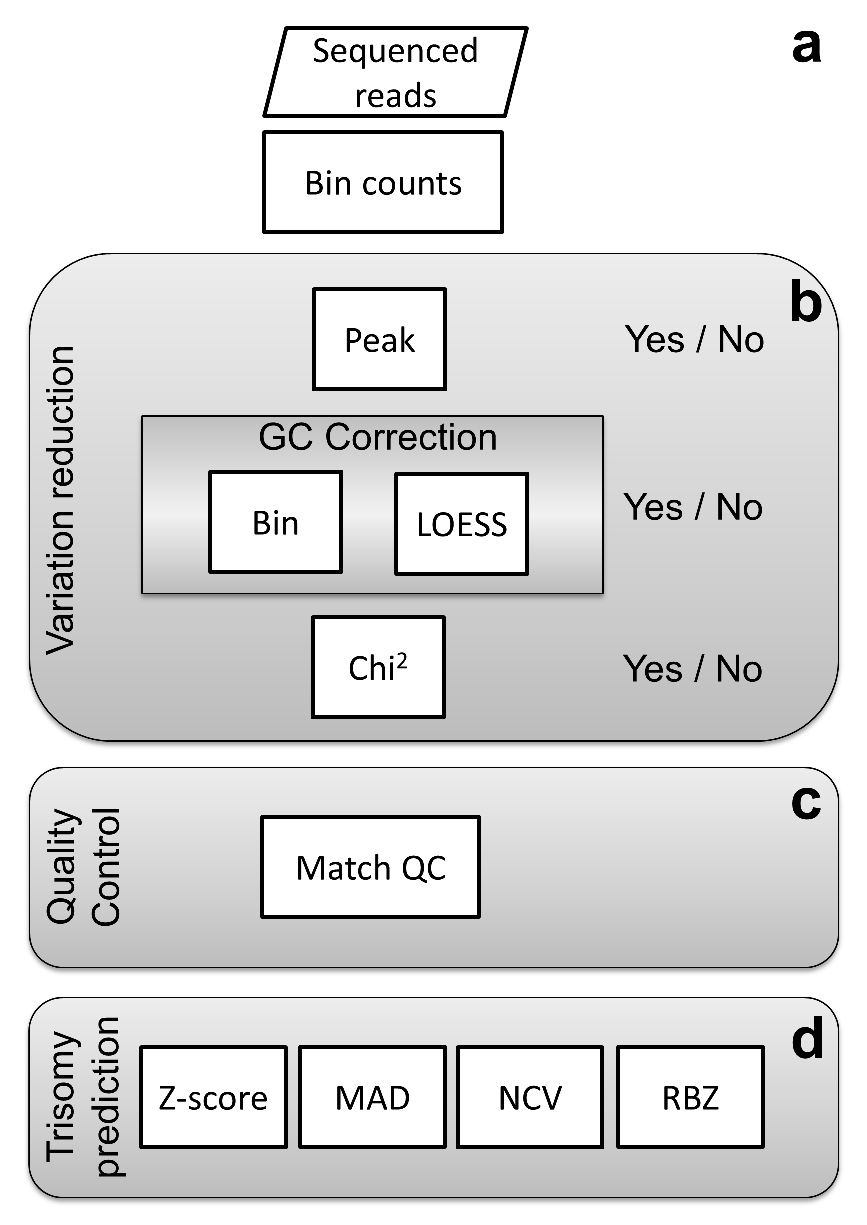
\includegraphics[width=0.6\linewidth]{img/Algorithms_NIPT_Fig1}
	\caption[Flowchart NIPT analysis steps]{Flowchart showing the analysis steps. \textbf{(a)} First, sequenced reads are aligned, partitioned into 50,000 bp bins and counted. These bins are the units for further analysis and data quality can be improved using zero or more variation reduction methods. \textbf{(b)} Peak correction removes bins showing an unusually high coverage compared with the average coverage of bins on the same chromosome. GC correction corrects for coverage differences between bins having a different GC percentage, using one of two methods: ‘bin’ or ‘LOESS’ GC-correction. The chi-squared variation reduction corrects bins showing a higher variation in read counts between samples than expected by chance. Analysis is performed based on (corrected) read counts. \textbf{(c)} The Match QC indicates whether a control-group is informative for the analyzed sample. \textbf{(d)} Various algorithms (standard Z-score, MAD-based Z-score, Normalized Chromosome Value and Regression-based Z-score) are used for predicting trisomy.}
	\label{fig:Algorithms_NIPT_Fig1}
\end{figure}

\subsection{Chi-squared-based variation reduction}
The novel $\chi$\textsuperscript{2}VR reduces the weight of the number of reads in bins that have a higher variation than expected by chance and thus reduces the impact of these bins on the chromosomal fractions. 
No prior knowledge on the origin of the variation is needed. 
The $\chi$\textsuperscript{2}VR performs a sum of squares calculation: per bin, the sum of the chi-squared value is calculated over all the selected control samples. 
For this calculation, the observed read counts $o$ are first normalized by multiplying them with a normalization factor. 
This factor is the mean number of observed total read counts for all autosomal bins $i$ of all control samples $j$ divided by the mean number of observed total read counts for all autosomal bins of the sample $s$. 
In short, the observed normalized read count for a specific bin ($on_i$ ) can be calculated as follows:

\begin{equation*}
	on_{is} = o_{is} \times \frac{(\sum^n_{ij=1}o_{ij})) / (n_i \times n_j)}{(\sum^n_{i=1}o_{is})/n_i}
\end{equation*}


\noindent where $n_i$ is the number of bins and $n_j$ is the number of control samples. 
Then, the chi-squared value for each bin $i$ is calculated for each control sample $j$ by dividing the squared difference between the expected and observed normalized read count by the expected normalized read count for that bin, where the expected normalized read count is the average normalized read count for a specific bin in all control samples ($\mu_{ij}$). 
The sum chi-squared value is calculated by adding up the chi-squared values of all the control samples for the bin:

\begin{equation*}
	\sum^n_{j=1}\chi_{ij}^2 = \frac{(\mu_{ij} - on_{ij})^2}{\mu_{ij}}
\end{equation*}

\noindent The sum chi-squared value for each bin is transformed to a standard normal distribution $N(0, 1)$ by subtracting the degrees of freedom $df$ (number of control samples minus one) from the sum chi-squared value and dividing this by the square root of two times the degrees of freedom.

\begin{equation*}
	N(0,1) = \frac{(\sum^n_{j=1}\chi_{ij}^2) - df} {\sqrt{2df}}
\end{equation*}

\noindent This results in a Z-score, which shows the number of standard deviations (SD) an observation differs from the expectation. 
Reads in bins with a Z-score higher than 3.5 are divided by the sum chi-squared value divided by the degrees of freedom, thereby reducing the variability between the samples. 
Normalized read counts in bins with a Z-score lower than 3.5 are not corrected. 
The justification for this procedure is that probability plots show the expected chi-squared distribution up to a Z-value of about 3.5. 
Values above 3.5 are much more frequent than would be expected, so instead of ignoring those bins we chose to reduce the weights, assuming that there is still information present in the over-dispersed bin counts. 
An overview of the analysis steps and their effects is shown in Supplement 1\footnote{added at the end of this chapter}.

\subsection{Regression-based Z-score}
The RBZ combines linear regression with a Z-score calculation. 
In the RBZ calculation the fraction of the chromosome of interest is predicted using stepwise regression with forward selection, in short forward regression. 
The reads aligned to the forward and reverse strands are used as separate predictors, because several chromosomes show a small, but consistent, over- or underrepresentation of reads aligned to the forward or reverse strand (Supplement 2). 
However, all reads aligned to the chromosome of interest are taken together rather than separated, because the higher number of reads leads to a lower variability in the number of reads aligned to the chromosome of interest.

For each chromosome of interest, the four best predictor sets, which each consist of four predictors, are determined by forward regression, using the adjusted R squared of the model as a selection criterion. 
The predictors can have either a positive or a negative correlation with the chromosome of interest. 
Within each predictor set only one predictor can be selected from each chromosome, limiting the risk of introducing bias.

Using the models created for each control sample s the expected chromosomal fraction ($ef$) is calculated for the chromosome of interest. 
Subsequently, the observed chromosomal fraction of the total read count of the chromosome of interest ($of$) is divided by this expected fraction. 
In combination with the standard deviation of the prediction, a Z-score is calculated for each sample. 
Because the mean of the control group after regression is one, the coefficient of variation of the control group has the same value as the SD.

In short, the RBZ can be formulated as:

\begin{equation*}
	\frac{of_s / ef_s - 1}{\sqrt{\sum^n_{j=1}(of_j / ef_j - \overline{of/ef})^2 / n - 1}}
\end{equation*}

\noindent where $s$ is the sample of interest, $j$ is an individual control sample and $n$ is the total number of control samples.

The RBZ not only uses information from chromosomes having a positive correlation of read counts with the chromosome of interest, but also from chromosomes showing a negative correlation. 
An overview of an example RBZ calculation is shown in Supplement 3\footnote{added at the end of this chapter}.

\subsection{Match QC score}
For the sample of interest, the novel Match QC score algorithm calculates how well the overall pattern of chromosomal fractions matches the pattern of the control samples. 
If the pattern of the sample differs too much from that of the controls, the sample does not fit within the control group, making the control set non-representative for the sample. 
Cut-offs are control-group-specific and can be set using the Match QC scores of the individual control group samples. 
The Match QC score uses the data used for trisomy prediction as input. 
Variation reduction, e.g. GC-correction or $\chi$\textsuperscript{2}VR, is applied before calculating the Match QC score.

To obtain the Match QC score, first the chromosomal fractions ($of$) are calculated for the sample and all control samples. 
This is done by dividing the (weighted or corrected) total read count of each chromosome by the total read count of all autosomal chromosomes, excluding chromosomes 13, 18 and 21. 
Subsequently, for each control sample, the sum of squared differences of the chromosomal fractions between the sample and the control for all autosomal chromosomes, excluding chromosomes 13, 18 and 21, is calculated.

In short, the Match QC score between a sample of interest $s$ and an individual control sample $j$ can be formulated as:

\begin{equation*}
	\sum^n_{k=1}(of_{ks} - of_{kj})^2
\end{equation*}

\noindent where $k$ is the chromosome and $m$ is the total number of chromosomes, excluding chromosomes 13, 18 and 21.

Smaller differences indicate a better match. 
An overall Match QC score is calculated by taking the average of the results of all samples. The formula for the overall Match QC score is:

\begin{equation*}
	\frac{\sum^n_{j=1}\sum^m_{k=1}(of_{ks} - of_{kj})^2}{j}
\end{equation*}

\noindent where $n$ is the number of control samples.

\subsection{Validation of algorithms}
\subsubsection{Samples}
To assess the effects of different variation reduction and trisomy prediction algorithms, we sequenced 128 non-trisomy and 43 trisomy samples using the SOLiD Wildfire platform (Life Technologies, Carlsbad, CA, USA) and 142 non-trisomy and 7 trisomy samples using the HiSeq 2500 platform (Illumina, San Diego, CA, USA). 
A further 34 non-trisomy samples had an alternative plasma-isolation and were sequenced on a HiSeq. 
The trisomy status of all samples was determined using karyotyping or quantitative fluorescence PCR following amniocentesis or chorionic villi biopsy.

Samples were selected in accordance with and as part of the \underline{tri}al by \underline{D}utch laboratories for \underline{e}valuation of \underline{n}on-invasive prenatal \underline{t}esting (TRIDENT) program, supported by the Dutch Ministry of Health, Welfare and Sport (11016-118701-PG). 
The program was also approved by the Ethics Committee of the University Medical Center Groningen. 
All participants signed an informed consent form.

\subsubsection{Plasma isolation, sample preparation and sequencing}
Plasma was obtained from two different sources. 
The first source was fresh EDTA blood, either processed within 3 hours of blood collection or within 24 hours if stabilizing reagent was present in the tubes (Streck Inc., Omaha, NE, USA). 
For samples sequenced using the Illumina platform, blood was first centrifuged at 1200 rcf for 10 minutes, without using brakes to stop the rotor. 
The plasma was then transferred to another tube and centrifuged at 2400 rcf for 20 minutes. The plasma was transferred to a third tube and stored at -80 $\degree$C. 
For samples sequenced on the SOLiD platform, the centrifugal forces used were 1600 rcf and 16000 rcf, respectively. 
The second source of plasma was obtained using an alternative isolation method using only the first centrifugation step at 1200 rcf, after which the blood plasma was stored at -20 $\degree$C.

For samples sequenced on the HiSeq, we isolated cell-free DNA (cfDNA) from 1.5 ml plasma with the QIAamp MinElute Virus Spin kit (Qiagen, Valencia, CA, USA) (90 non-trisomy and 6 trisomic samples), the Qiagen circulating nucleic acid kit (Qiagen) (21 non-trisomy samples) and the Akonni TruTip kit (Akonni Biosystems, Frederick, MD, USA) (31 non-trisomy samples and 1 trisomic sample). 
After DNA isolation, sample preparation was performed with NEBNext Multiplex Oligos for Illumina (New England Biolabs Inc., Ipswich, MA, USA). 
Before the amplification step, we performed a two-step size selection using Agencourt AMPure xp beads (Beckman Coulter, Inc., Brea, CA, USA), using a beads/sample ratio of 0.6:1 in the first step and a ratio of 1.2:1 in the second step. Samples were sequenced with a 50 bp read length on a HiSeq 2500 sequencing platform (Illumina).

For samples sequenced on the SOLiD, cfDNA was extracted from 1 ml plasma using the QIAamplDSP DNA blood mini kit (Qiagen). 
Libraries were prepared according to factory protocol and sequenced with a 35 bp read length on the SOLiD 5500 Wildfire sequencing platform (Life Technologies).

\subsubsection{Read alignment}
For Illumina data, after an initial quality control of the fastq data using the program fastqc (v.0.7.0), the data were aligned to the human reference genome build b37 as released by the 1000 Genomes project \cite{Durbin_2010} using BWA aln samse (0.5.8\_patched) with default settings \cite{Li_2010}. 
After alignment a Sam output file \cite{Li_2009} was created for each sample. 
Using Picard tools 1.6.1, a set of tools designed by the Broad Institute (Cambridge, USA) (http://broadinstitute.github.io/picard/) for processing and analyzing next generation sequencing data, the Sam files were transformed into Bam files. 
These Bam files were sorted and Bam index files formed. 
The Bam index files link the reads to the genome position. 
Quality metrics files were then created and the duplicate reads in the Bam files marked.

For SOLiD data, raw reads were mapped against the human reference genome (GRCh37/hg19) using BWA v0.5.913. 
Options used for mapping were -c, -l 25, -k 2, and -n 10. 
The Bam files were filtered using Sambamba v0.4.5 \cite{Tarasov_2015} to retain non-duplicate reads, uniquely mapped reads (XT:A:R), reads with no mismatches to the reference genome (CM:i:0), and reads with no second best hits in the reference genome (X1:i:0).

After filtering and removal of duplicate reads, the total autosomal read count was on average 20.2 million (SD 5.6 million) for SOLiD data and 12.5 million (SD 2.2 million) for Illumina data.

\subsubsection{Variation reduction}
Aligned reads were divided into 50,000 bp bins and variation between samples was reduced using all possible combinations of zero or more variation reduction methods: peak correction, GC-correction and $\chi$\textsuperscript{2}VR. 
When more than one method was used, they were performed in the order described above (Fig. 1). 
A maximum of one GC-correction method was used. Since the LOESS GC-correction has been described more often \cite{Chen_2011,Lau_2012,Palomaki_2012,Liang_2013} than the weighted bin GC-correction \cite{Fan_2010}, we used LOESS GC-correction to evaluate the other variation reduction and prediction methods.

\subsubsection{Peak correction}
Peak correction was performed as described by Fan and Quake \cite{Fan_2010}. 
This method removes bins having a read count that significantly differs from the average using the information of all control samples. 
A bin was considered to deviate from normal if the total read count fell outside 1.96 SD compared with total read counts in the bins on the same chromosome for that sample. 
We interpreted bins to have a consistent pattern of region-specific variations if the variation deviated from normal in 95\% or more of the control samples.

\subsubsection{GC-correction}
An important factor explaining the systematic uncontrolled variation between chromosomes is the guanine and cytosine (GC) content of the DNA fragments analyzed. 
When this GC-bias is corrected during preprocessing of the data, it results in a significantly lower variability \cite{Liang_2013}. 
GC-correction was performed based on total read counts using two different methods. 
The first GC-correction method is based on a LOESS curve fitted to the reads counts in bins sorted on GC content \cite{Chen_2011,Lau_2012,Palomaki_2012,Liang_2013} and based on R v3.0.2 default settings (span 0.75; degree = 2). 
The second GC-correction method is based on the average coverage of bins having a similar GC-content \cite{Fan_2010}. 
The GC\% of each bin is determined for both methods. Bins not containing any reads and bins with an unknown base composition are ignored. 
The weights of the correction factors were based on GC-content intervals of 0.1\% and consisted of the average coverage of the bins within the GC-interval divided by the average coverage of all bins.

\subsubsection{Trisomy prediction}
We predicted trisomies using four different prediction methods: standard Z-score prediction \cite{Chen_2011}, NCV, using only the most informative chromosomes \cite{Sehnert_2011}, MAD-based Z-score \cite{Stumm_2013} and RBZ. 
Depending on the variation reduction methods employed, we used corrected or uncorrected read counts for prediction. 
For all analyses chromosomes 13, 18 and 21 were not used as predictor chromosomes, since the prediction would be affected if a trisomy was present in one of the chromosomes used for prediction.

In short, the standard Z-score calculates the fraction of reads originating from the chromosome of interest compared with all reads originating from autosomal chromosomes, and then subtracts the mean fraction – which is the expected fraction – of the chromosome of interest in a set of control samples. 
The result is then divided by the SD of the fraction in the control set.

The NCV does not use all the autosomal chromosomes to calculate the fraction of the chromosome of interest, instead using the most informative chromosomes, which were selected using a training set \cite{Sehnert_2011}. 
All combinations of denominator chromosomes were tested for both the Illumina and SOLiD datasets, and the combinations yielding the lowest CVs were selected. 
The NCV is sometimes compared to using an internal reference \cite{Lau_2012} because, during analysis, the selected reference chromosomes behave similarly to the chromosome of interest. 
This positive correlation results in less sample to sample variation, reduces the need for GC correction, and increases prediction precision.

The MAD-based Z-score replaces the SD by 1.4826 * MAD, making the calculation more tolerant of outliers in the control set \cite{Stumm_2013}. 
The MAD was calculated in three steps. 
First, the median of the fractions of the chromosome of interest in the control set was calculated. 
Second, the absolute difference of the chromosomal fraction to the median was calculated for each control sample. 
Finally, the MAD was calculated by taking the median of these absolute differences.

\subsubsection{Comparison of the algorithms}
In comparing the algorithms we used the CV as a benchmark for performance. 
The CV is a standardized measure of dispersion of a probability distribution and is defined as the ratio of the SD to the mean. 
In this manner it enables comparison between normal distributions with a different mean. 
The height of the CV of the control group, together with the percentage cffDNA, determines the discriminative power between normal and trisomic samples. 
When the CV decreases, the sensitivity increases (Supplement 4). 
We determined the added value of each variation reduction or prediction algorithm to lowering the CV to determine the best combination of algorithms.

For our analysis, we used all the non-trisomy samples sequenced with the same platform that underwent the same plasma isolation procedure as control samples. 
This resulted in control group sizes of 142 for the Illumina and 128 for the SOLiD sequencer. 
For all algorithms, the control group is only used when it is normally distributed as determined using the Shapiro Wilk statistical test (p \textgreater\: 0.05).

\subsubsection{Algorithm combinations tested}
We evaluated the effects of both peak correction and $\chi$\textsuperscript{2}VR on the CV of the control samples, the effect of the two different GC correction methods in combination with all prediction methods on the CV, and the effect of the different prediction methods on CV and Z-scores in combination with all possible variation reduction methods, except peak correction and the bin GC correction. 
The consistency of the RBZ trisomy prediction was determined by estimating three additional trisomy prediction models for each analysis.

\subsubsection{Match QC score}
To provide a proof of principle for the Match QC score performance, we divided the Illumina control group into a training set of 85 and a test set of 57 samples. 
The 34 Illumina samples that underwent a different plasma isolation protocol were used as an example of samples having undergone an alternative procedure.

We then calculated the Match QC score for all samples, using uncorrected, $\chi$\textsuperscript{2}VR, LOESS GC, and combined LOESS GC and $\chi$\textsuperscript{2}VR-corrected data. 
Cut-offs for the Match QC score were set on the average Match QC of the training set plus three SD. 
For all samples Z-scores were calculated for chromosomes 13, 18 and 21 to determine whether the scores fall within three SD of the average of the control set.

\section{Results}\label{Results}
For both the SOLiD and Illumina control groups, the CV of chromosomes 13, 18 and 21 was determined for all combinations of variation reduction and trisomy prediction methods and their theoretical effect on sensitivity and specificity was calculated (Supplement 5). 
The estimated percentages of cffDNA in the tested trisomy samples are shown in Supplement 6.

\subsection{Effect of peak correction}
To examine the effect of correcting bins with a coverage that deviates significantly from the average, we compared the CV of the peak-corrected data with that on which no peak correction was performed. 
Peak correction reduced the CV in most analysis strategies (Fig. \ref{fig:Algorithms_NIPT_Fig2}). 
The largest relative effect for all chromosomes was observed when a GC-correction was also performed. 
The effect was largest in chromosome 21, which was the chromosome showing the lowest GC-bias when no correction was applied, suggesting that the influence of coverage peaks on variability only comes to light when GC-bias is limited. 
In data that was also $\chi$\textsuperscript{2}VR corrected, the variation did not further decrease but it did sometimes increase after use of a peak correction. 
This suggests that the peak correction and the $\chi$\textsuperscript{2}VR are partly correcting the same sources of bias.

\begin{figure}
	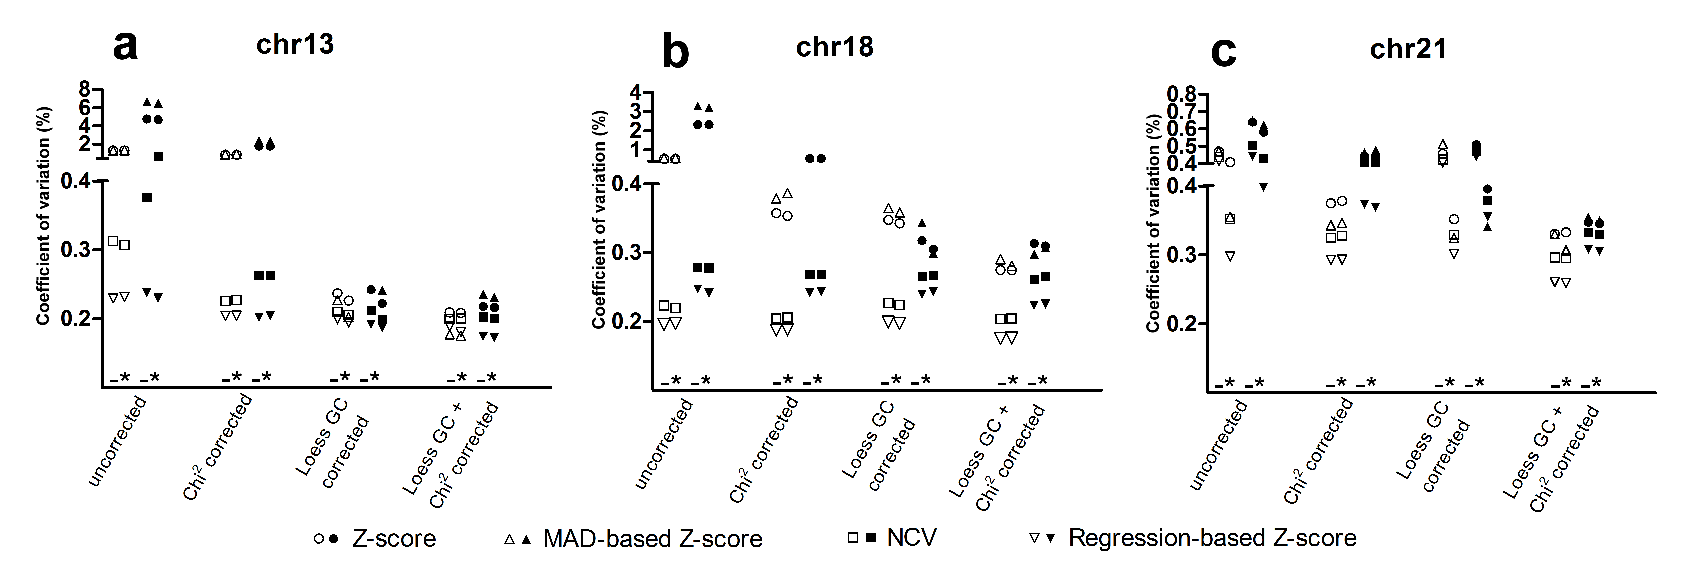
\includegraphics[width=1.0\linewidth]{img/Algorithms_NIPT_Fig2}
	\caption[Effect of peak correction]{\textbf{Effect of peak correction on the CV of control samples}. The effect is shown for SOLiD (white) and Illumina data (black) with no other correction, for data that also had a chi-squared correction, or LOESS GC correction, or both LOESS GC and chi-squared correction. For each type of correction the CV of four prediction algorithms (standard Z-score, MAD-based Z-score, Normalized Chromosome Value and regression-based Z-score) are shown for \textbf{(a)} chromosome 13, \textbf{(b)} chromosome 18 and \textbf{(c)} chromosome 21. -not peak corrected; *peak corrected.}
	\label{fig:Algorithms_NIPT_Fig2}
\end{figure}

\subsection{Effects of the two GC correction methods}
To examine the performance of the weighted bin GC correction and the LOESS GC-correction, we compared the performance of both methods in combination with all other variation reduction and prediction methods for chromosomes 13, 18 and 21 (Fig. \ref{fig:Algorithms_NIPT_Fig3}) . 
For chromosome 13, both GC correction methods performed equally well regardless of the other variation reduction and prediction methods used. 
For chromosome 18, the weighted bin GC correction had a better performance for the NCV and RBZ compared to LOESS GC correction. 
However, the Z-score and MAD-based Z-score predictions performed better using the LOESS GC-correction. 
For chromosome 21, the weighted bin GC correction performed best, regardless of the other methods used. 
The data sets used made no difference to the performance of either GC-correction method.

\begin{figure}
	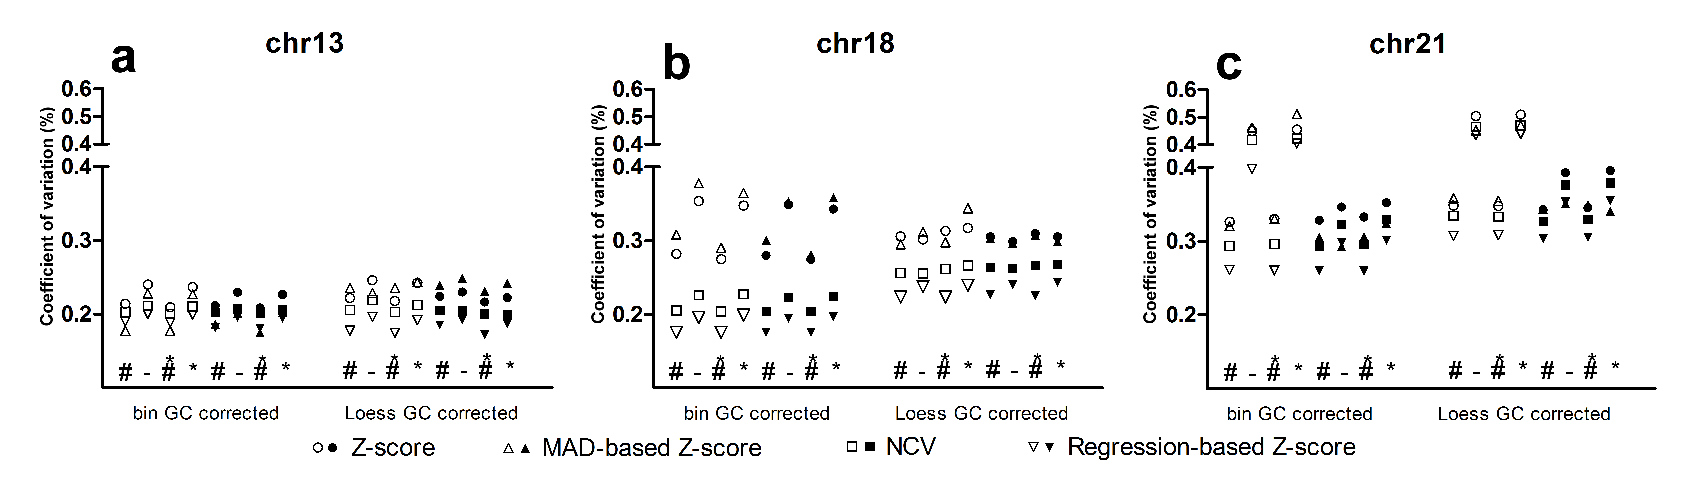
\includegraphics[width=1.0\linewidth]{img/Algorithms_NIPT_Fig3}
	\caption[Comparison of the effect of two GC correction methods]{\textbf{Comparison of the effect of two GC correction methods (bin GC correction and LOESS GC correction) on the CV of the control samples}. SOLiD data (white) and Illumina data (black). For each type of correction the CVs of four prediction algorithms (standard Z-score, MAD-based Z-score, Normalized Chromosome Value and regression-based Z-score) are shown for \textbf{(a)} chromosome 13, \textbf{(b)} chromosome 18 and \textbf{(c)} chromosome 21. \#Chi-squared corrected; -not corrected; *peak corrected.}
	\label{fig:Algorithms_NIPT_Fig3}
\end{figure}

\subsection{Effect of chi-squared-based variation reduction}
To examine the performance of the $\chi$\textsuperscript{2}VR, we compared the control group CV using all other variation and prediction methods, with and without the $\chi$\textsuperscript{2}VR (Fig. \ref{fig:Algorithms_NIPT_Fig4}).
The $\chi$\textsuperscript{2}VR resulted in a lower CV in most analysis strategies for all chromosomes. 
The effect was most striking in chromosome 21, regardless of the other methods used.

\begin{figure}
	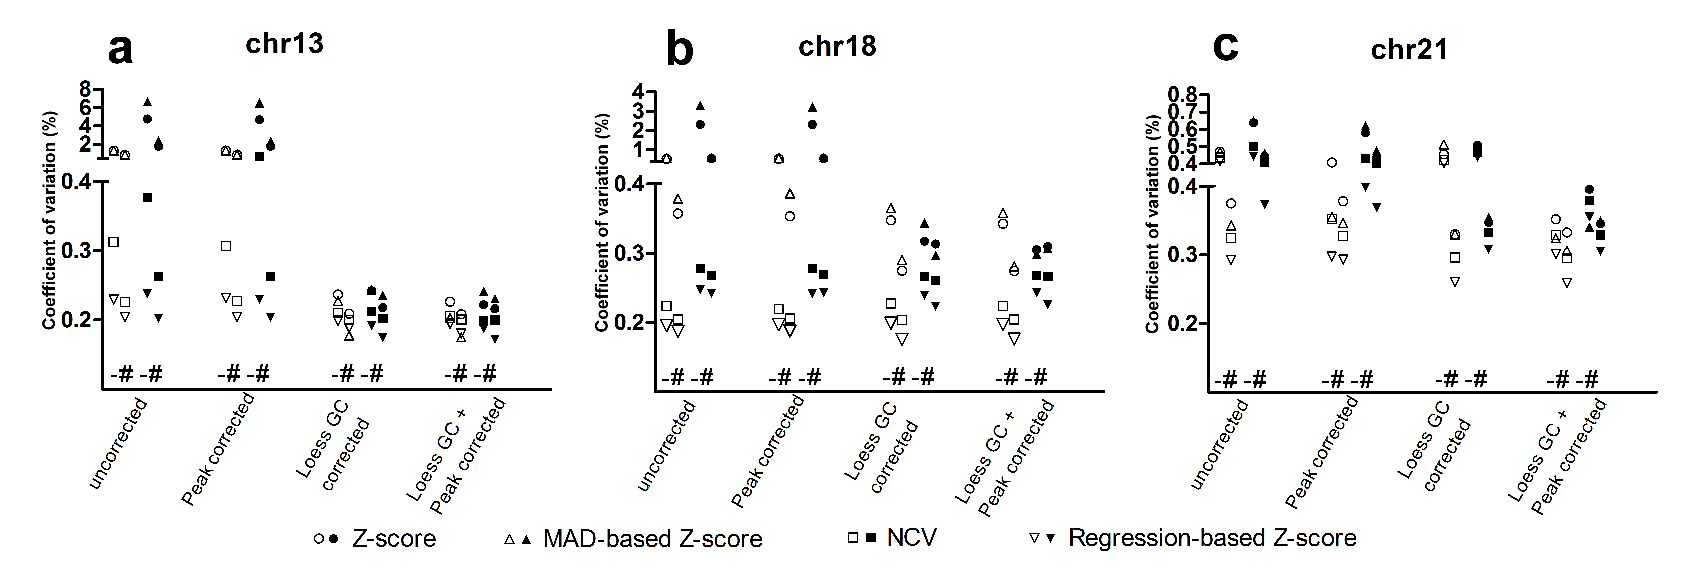
\includegraphics[width=1.0\linewidth]{img/Algorithms_NIPT_Fig4}
	\caption[Effect of chi-squared-based variation reduction control samples CV.]{\textbf{Effect of chi-squared-based variation reduction on the CV of control samples}. SOLiD (white) and Illumina data (black) with no other correction, or with a peak correction, or LOESS GC correction or both LOESS GC and peak correction. For each type of correction the CVs of four prediction algorithms (standard Z-score, MAD-based Z-score, Normalized Chromosome Value and regression-based Z-score) are shown for \textbf{(a)} chromosome 13, \textbf{(b)} chromosome 18 and \textbf{(c)} chromosome 21. –not chi-squared corrected; \#chi-squared corrected.}
	\label{fig:Algorithms_NIPT_Fig4}
\end{figure}

\subsection{Effect of trisomy prediction algorithms}
To examine the effect of the prediction algorithms (standard Z-score, MAD-based Z-score, NCV and RBZ), we compared the CV using uncorrected, $\chi$\textsuperscript{2}VR, LOESS GC, and combined $\chi$\textsuperscript{2}VR and LOESS GC corrected data. 
Since the peak correction provides no added value to the $\chi$\textsuperscript{2}VR, it was not used for comparison. 
The RBZ produced the lowest CV for all variation reduction methods except the SOLiD combined LOESS GC and $\chi$\textsuperscript{2}VR corrected data, in which the MAD-based Z-score for chromosome 13 produced an even lower CV (Fig. \ref{fig:Algorithms_NIPT_Fig5}). 
The variation using the NCV is higher than that using the RBZ, but the CV is still much lower than the CVs of the methods that used all autosomal chromosomes. 
The standard Z-score had the highest coefficient of variation in all models.

\begin{figure}
	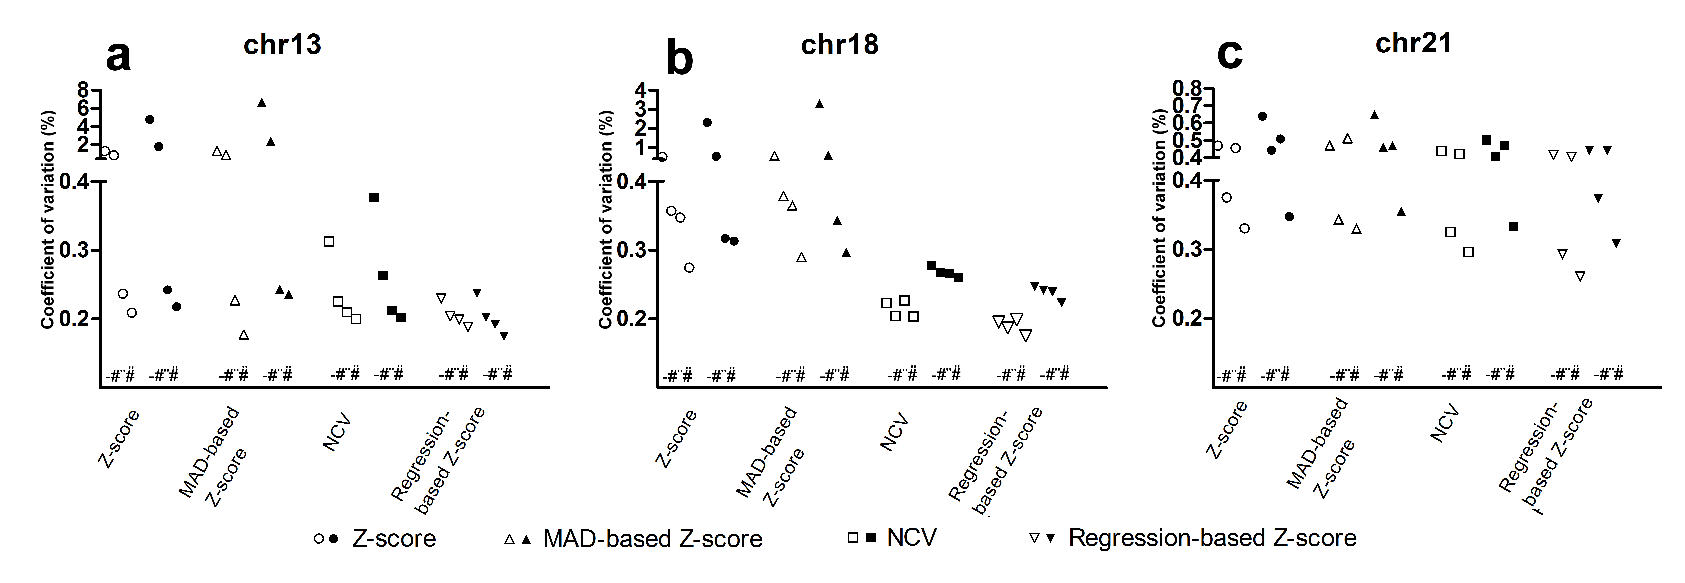
\includegraphics[width=1.0\linewidth]{img/Algorithms_NIPT_Fig5}
	\caption[Effect of the different prediction algorithms]{\textbf{Effect of the different prediction algorithms on the CV of control samples}. SOLiD data (white) and Illumina data (black). Results from the four different prediction algorithms (standard Z-score, MAD-based Z-score, Normalized Chromosome Value and regression-based Z-score) are shown for \textbf{(a)} chromosome 13, \textbf{(b)} chromosome 18 and \textbf{(c)} chromosome 21. –Variation was not reduced, \#chi-squared corrected, “ LOESS GC corrected, \#” both LOESS GC and chi-squared corrected before prediction.}
	\label{fig:Algorithms_NIPT_Fig5}
\end{figure}

A lower CV yields a more extreme Z-score, which means that in the case of a trisomy, the Z-score is more likely to be higher than the threshold, resulting in a higher sensitivity. 
The Z-scores of the trisomy samples of the four prediction algorithms for the uncorrected, $\chi$\textsuperscript{2}VR, LOESS GC, and combined $\chi$\textsuperscript{2}VR and LOESS GC corrected data are listed in Supplement 7. 
False-negative and false-positive results were determined for all the above combinations of variation reduction algorithms and prediction algorithms, based on a 99.7\% confidence interval (Z-score threshold of three) (Supplement 8).

Of the 50 trisomic samples, a false-negative result was found in two trisomy 13 and three trisomy 18 samples for the Z-score or the MAD-based Z-score when no variation reduction was done. 
One confirmed trisomy 18 sample did not give a positive result with any combination of algorithms, possibly due to a low fetal percentage. 
No false-negatives were found for chromosome 21. 
For all true-positive results, all four RBZ models showed a Z-score higher than three.

To better show the effect of the different variation reduction and prediction algorithms on the Z-score, we selected three samples, sequenced on the SOLiD platform, each having a trisomy 13, 18 or 21 (Fig. \ref{fig:Algorithms_NIPT_Fig6}). 
Based on the Z-scores and CVs, each sample had an estimated fetal percentage of 5–6\%. 
The NCV and RBZ consistently yielded higher Z-scores than the standard Z-score and the MAD-based Z-score. 
The effect of the GC-correction is reflected in the results of the standard Z-score and the MAD-based Z-score for chromosome 13 and the effect of the $\chi$\textsuperscript{2}VR shows in the chromosome 21 results.

\begin{figure}
	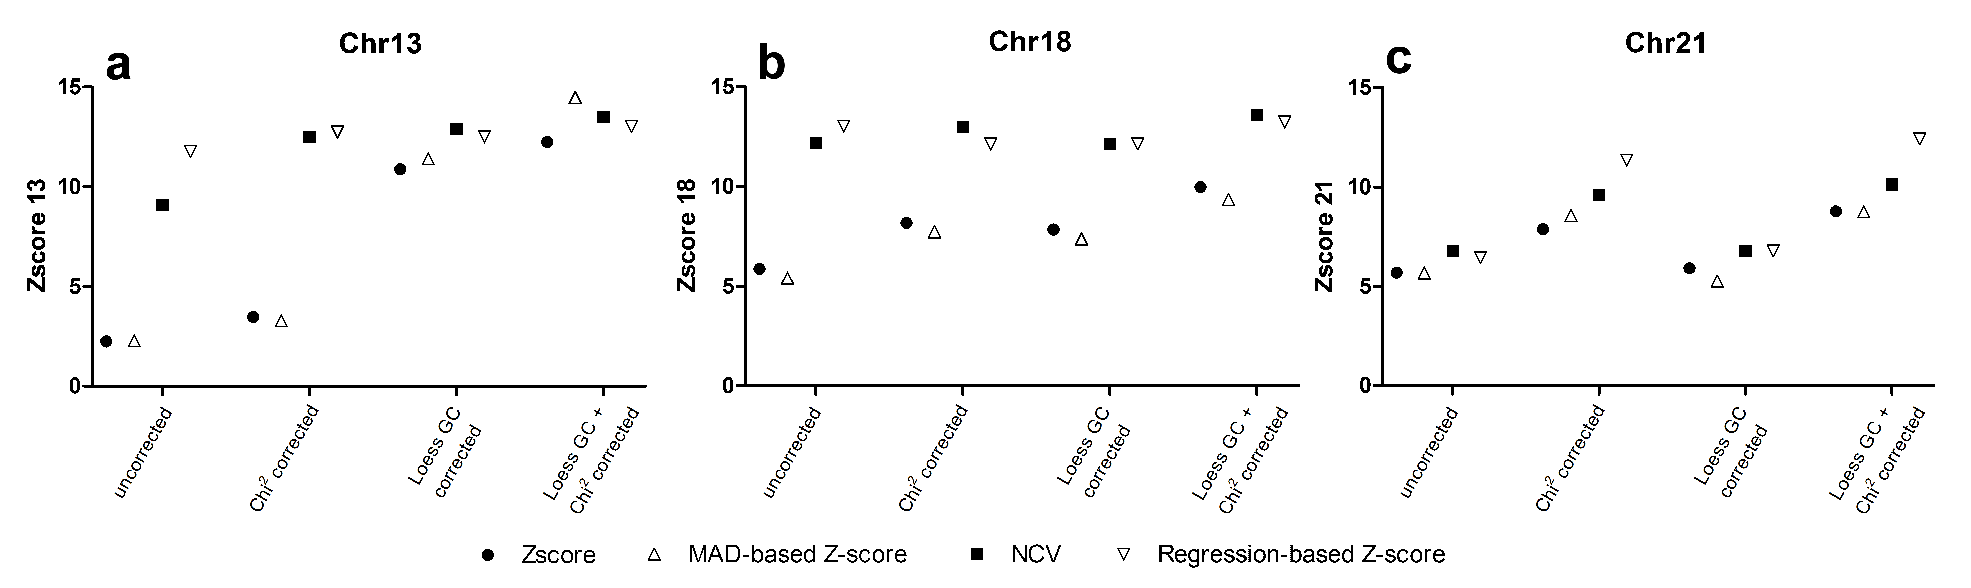
\includegraphics[width=1.0\linewidth]{img/Algorithms_NIPT_Fig6}
	\caption[Z-scores for three trisomies]{\textbf{Z-scores for three trisomies using different combinations of variation reduction and prediction algorithms}. All three examples are based on SOLiD data. Results from the four different prediction algorithms (standard Z-score, MAD-based Z-score, Normalized Chromosome Value, and regression-based Z-score), in combination with uncorrected, chi-squared corrected, LOESS GC corrected, and both LOESS GC and chi-squared corrected are shown for \textbf{(a)} chromosome 13, \textbf{(b)} chromosome 18 and \textbf{(c)} chromosome 21.}
	\label{fig:Algorithms_NIPT_Fig6}
\end{figure}

Of the 270 non-trisomy samples, four samples showed a false-positive result for more than one prediction algorithm. 
For one sample, all four prediction methods showed a result higher than three. The more sensitive NCV and RBZ prediction methods resulted in more false-positive results than the standard Z-score or MAD-based Z-score because more parameters are estimated, which leads to some overfitting and therefore underestimation of the prediction accuracy for new samples. 
This effect will be reduced when larger control groups are used. 
Three other false-positive results were only seen in one of the variation reduction methods, one for NCV and three for RBZ. In all these cases, Z-scores were just above three. 
In all cases adding or removing a variation reduction step, resulted in a negative call. 
For samples having a false-positive RBZ result, at least one of the additional RBZ predictions resulted in a negative prediction, except for the sample having a Z-score higher than three in all prediction methods.

\subsection{Match QC score}
To examine whether the Match QC score could accurately predict whether a sample fits within a control group, we calculated the Match QC scores and all the Z-scores for a training set, a test set of samples that had been prepared in the same manner as the training set, and a third set of samples originating from single centrifuged plasma. 
For all three sets, we used uncorrected, $\chi$\textsuperscript{2}VR, LOESS GC and combined $\chi$\textsuperscript{2}VR- and LOESS GC-corrected data (Fig. \ref{fig:Algorithms_NIPT_Fig7}). 
Test set samples had Match QC scores in the same range as the training set samples and Z-scores that fell within three SD of the mean for all types of corrected data. 
Single centrifuged samples, however, showed Match QC scores in the same range as the control group samples for uncorrected and $\chi$\textsuperscript{2}VR corrected data, but above the three-SD threshold for LOESS GC corrected data and combined LOESS GC- and $\chi$\textsuperscript{2}VR-corrected data.

\begin{figure}
	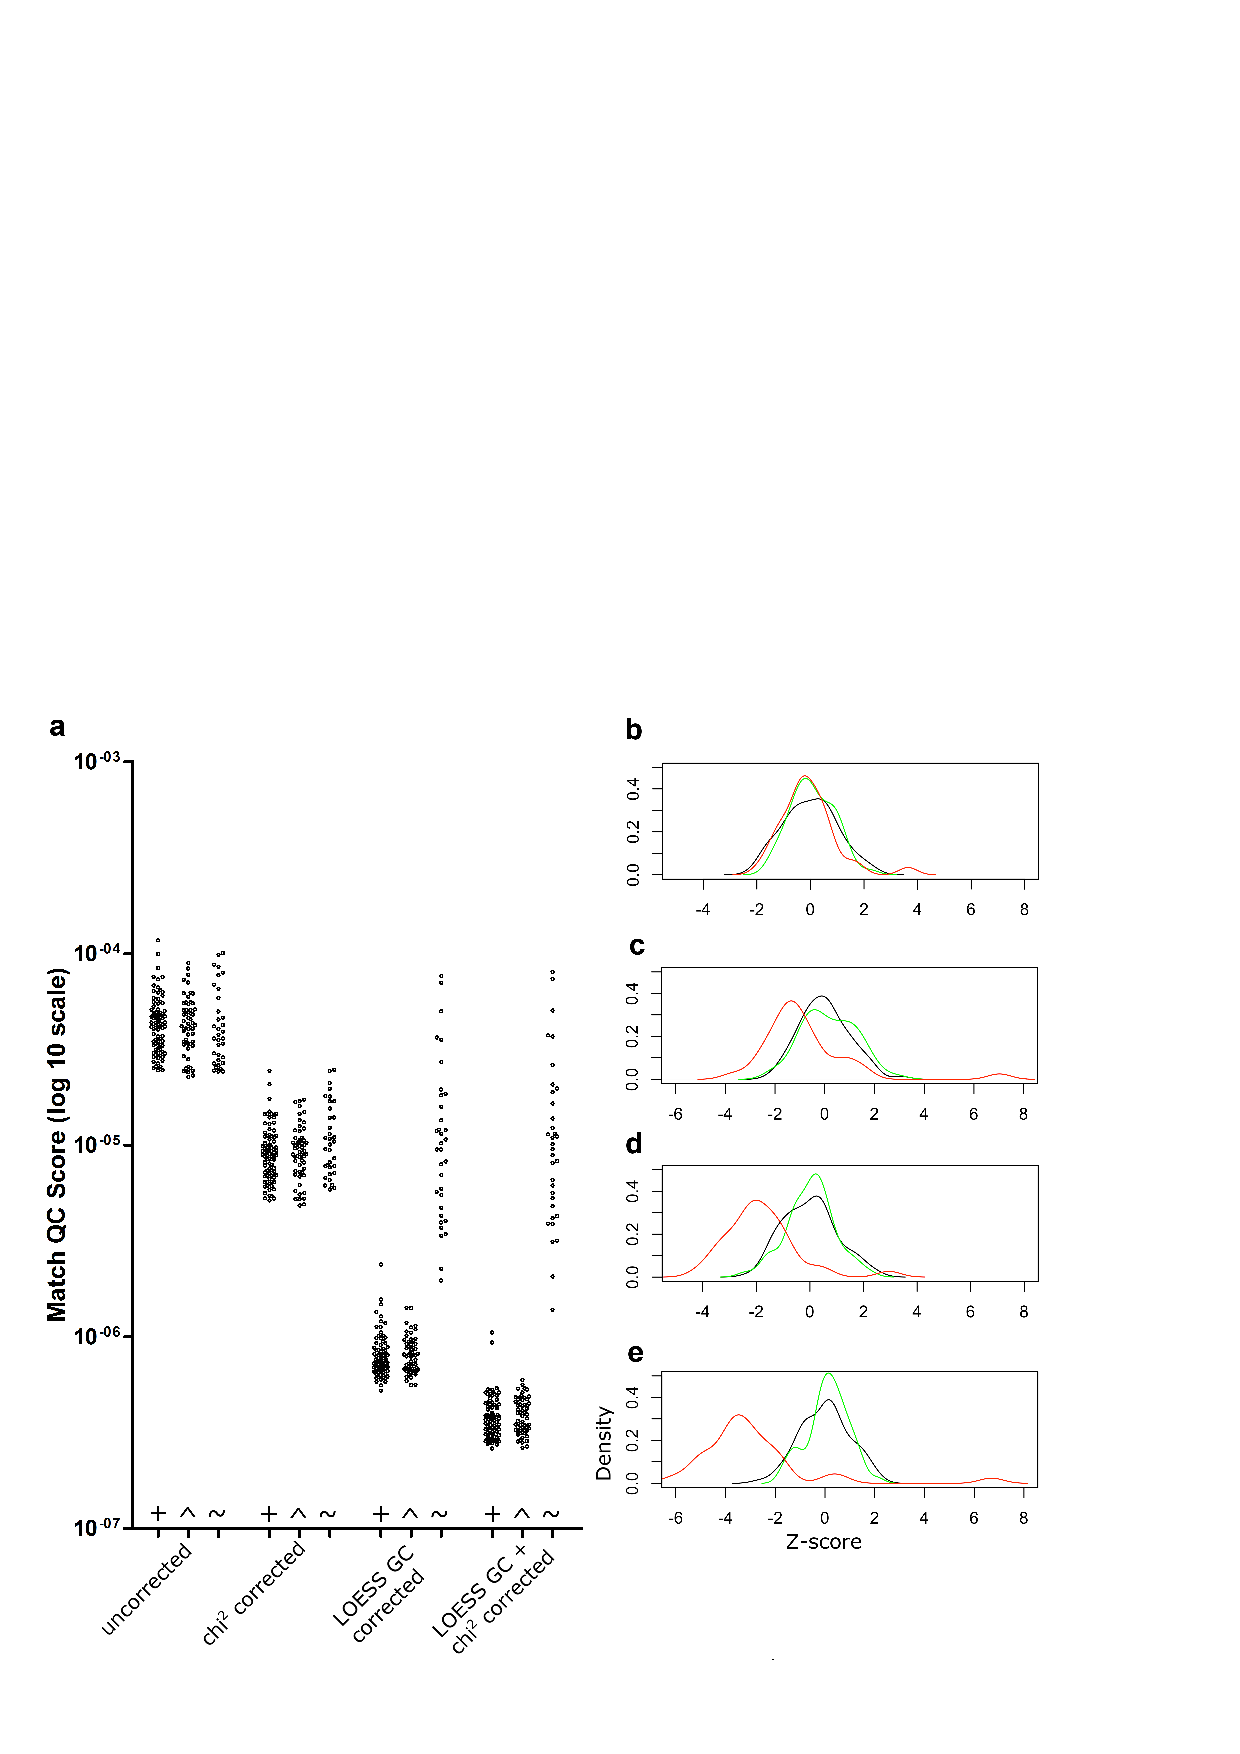
\includegraphics[width=0.8\linewidth]{img/Algorithms_NIPT_Fig7}
	\caption[Match QC scores and Z-scores]{\textbf{Match QC scores and Z-scores for matching and non-matching samples}. \textbf{(a)} Match QC scores per sample for uncorrected, chi-squared corrected, LOESS GC corrected and both LOESS GC and chi-squared corrected data for the control group, matching samples, and non-matching samples. Chromosome 21 Z-scores for \textbf{(b)} uncorrected data, \textbf{(c)} chi-squared corrected data, \textbf{(d)} LOESS GC corrected data and \textbf{(e)} both LOESS GC and chi-squared corrected data. + and black line, control group samples; $\wedge$ and green line, samples that underwent the same sample preparation procedure; $\sim$ and red line, single centrifugation plasma samples.}
	\label{fig:Algorithms_NIPT_Fig7}
\end{figure}

Z-score distributions for the training set samples and the test set samples were indistinguishable for all correction methods, but Z-scores based on uncorrected or $\chi$\textsuperscript{2}VR corrected data were not normally distributed for chromosomes 13 and 18. 
For the single centrifuged samples, Z-scores did not deviate from the normal distribution for the uncorrected data of chromosome 21. 
Match QC scores for all the samples analyzed, thresholds and Z-score distributions for chromosomes 13, 18 and 21 are shown in Supplement 9.

\section{Discussion}\label{Discussion}
We show that both the $\chi$\textsuperscript{2}VR and the RBZ reduced the variability of the NIPT result and thus increased its sensitivity in both Illumina and SOLiD data. 
Furthermore, we show that a Match QC exceeding a three-SD threshold, determined using control samples, identified those samples for which the controls were not representative. 
Although the algorithms described in this study are designed to improve analysis of NIPT data, they may also be of use in similar types of analyses that need high sensitivity such as copy number variation detection in liquid biopsy data \cite{Chan_2012,Leary_2012}.

The lower variability between samples decreases the percentage of fetal DNA needed for NIPT. 
A low percentage of fetal DNA is an important contributor to false negative or inconclusive results \cite{Mackie_2016}. 
Moreover, the average percentage of fetal DNA is lower in trisomy 13 and trisomy 18 pregnancies than in non-trisomy pregnancies \cite{Wegrzyn_2006,Ashoor_2012a}. 
A low variability is therefore even more important for these pregnancies for the test to have a high sensitivity. 
Moreover, our novel algorithms produce a lower variability for a given number of reads, resulting in the need for fewer reads and lowering sequencing costs. 
Alternatively, only DNA-fragments originating from regions of interest could be selected \cite{Sparks_2012b,Ashoor_2013,Zimmermann_2012}. 
However, such a selection requires additional amplification during sample preparation, which could also create additional variation due to increased over-dispersion \cite{Mutter_1995,Dohm_2008}. 
We therefore chose to reduce variation by correcting for bias in read counts before analysis, leading to a more comparable distribution of reads over the chromosomes between samples. 
Other studies have shown that variability can be introduced by bias present in the data, such as GC-bias \cite{Fan_2008,Chen_2011,Lau_2012,Palomaki_2012,Liang_2013,Fan_2010}, or peaks of extreme coverage, probably caused by repeats \cite{Fan_2010}. 
However, due to a higher number of available reads, better results were obtained using a non-repeat-masked reference genome \cite{Chen_2011,Palomaki_2012}. 
For this reason, we did not mask any regions based on mappability tracks or blacklisted regions in our comparison.

In our comparison the lowest CVs for chromosomes 13, 18 and 21 were produced using the combination of the weighted-bin-based GC-correction method and the $\chi$\textsuperscript{2}VR with the RBZ. 
However, each variation reduction algorithm we tested reduced the variability when used alone. 
The effect of the peak variation reduction was small when combined with the $\chi$\textsuperscript{2}VR. 
This shows that the $\chi$\textsuperscript{2}VR corrects bias caused by regions of extreme coverage. 
Moreover, since the $\chi$\textsuperscript{2}VR focuses on variation present in each specific bin, and not on chromosomal averages, it can correct for variation that is too subtle for peak correction. 
And since no assumptions are made about the origin of the bias, no prior knowledge is needed for correction. 
However, when using the$\chi$\textsuperscript{2}VR on the X-chromosome, variability should be determined using only data from pregnancies of a female fetus to prevent variability in the fetal percentage adding to the total variability on that chromosome. 
After application of GC-correction, $\chi$\textsuperscript{2}VR reduced variation even further, suggesting that $\chi$\textsuperscript{2}VR corrects for sources of bias other than that from GC. 
Since up to 50\% of the human genome is repetitive \cite{Smit_2013}, we suggest that part of the extra corrected bias is due to repeat structures. 
It has also been suggested that biological factors play a role in bias in NIPT \cite{van_den_Oever_2013,Chandrananda_2014}, so part of the corrected bias might have a biological origin.

Where peak correction and $\chi$\textsuperscript{2}VR only remove reads to reduce variation, GC-correction removes reads in bins having a GC-percentage containing more reads than average, but it adds virtual reads in bins with a GC-percentage containing fewer reads than average. 
Although, after GC correction, more reads seem to be present for several chromosomes, dispersion is still based on the original number of reads aligned to those chromosomes.

We demonstrated that the prediction method used can also reduce variability and increase sensitivity. 
The RBZ resulted in the lowest variability and decreased the need for GC-correction because this method takes this kind of systematic bias into account. 
However, there may be some pitfalls. 
Similar to the NCV, prediction is based on a limited number of predictor chromosomes. 
The effect of an aberration in one of the predictor chromosomes on the prediction is larger for the RBZ and NCV than for the standard Z-score, which uses all autosomes for prediction. 
To limit the effect of possible aberrations, we recommend comparing four independent predictor sets for the RBZ. Conflicting results of different models are a warning of possible false-positive results. 
In our data, all 49 trisomies detected were predicted independently by the four RBZ prediction sets. 
Only one false-positive call was made by all four sets. 
This call was also made by all the other prediction methods, suggesting that there may indeed be a higher fraction of reads of the called chromosome present in the data. 
Since the NCV can be based on only one denominator chromosome, we suggest multiple predictions using different denominators should also be used for NCV.

Our results show that a Match QC score below the three-SD threshold does not guarantee that the control group is representative for a sample, but a score exceeding the threshold does indicate that the analysis is not accurate. 
The main assumption in NIPT analysis is that the control set is representative of the sample analyzed. 
A non-representative control set leads to an inaccurate prediction and possibly to false-positive or false-negative results. 
It is therefore important that all samples undergo the same preparation, sequencing procedure and bioinformatics analysis. 
However, even when standard procedures are used, bias can vary between sequencing runs \cite{Aird_2011}. 
Prediction methods with a higher sensitivity are more vulnerable to the effects of unaccounted biological variation because deviations in the expected chromosomal fractions will more rapidly lead to false-positive results. 
Sample quality metrics are therefore essential for reliable analysis.

Our study shows that both the $\chi$\textsuperscript{2}VR and the RBZ increase the sensitivity of NIPT compared to previously published methods. 
Furthermore, we show that the Match QC score identifies samples for which the non-trisomy control set was not informative. 
Moreover, these algorithms may have a broader applicability than NIPT analysis, for instance in analysis of copy number variations in liquid biopsy data. 
We recommend our novel algorithms, as included in the NIPTeR package, as a useful addition to the NIPT analysis toolbox, resulting in a higher sensitivity, in theory making it possible to detect trisomies in blood with a fetal DNA amount as low as 2\%.

\section*{Acknowledgments}\label{Acknowledgments} 
We thank Jackie Senior and Kate Mc Intyre for editorial advice.

\subsubsection{Author contributions}
L.F.J. and E.N.d.B. wrote the manuscript and prepared the figures. L.F.J., E.N.d.B. and G.J.t.M. developed the methods and performed validation studies. H.A.d.W., L.F.J., F.v.D. and M.G.E. built the software packages and analysis pipeline. G.H.S.-B., R.F.S. and B.S. included the patients. R.J.S., G.J.t.M., R.H.S., M.A.S. and B.S. supervised the design and progress of this project. All authors read and approved the final manuscript.

\subsubsection{Competing interests}
The authors declare that they have no competing interests.

\section*{Supplementary material}\label{Supplementary material}
Supplements 1 and 3 are added as an addendum to this chapter. 
The other supplements can be accessed online: 

\noindent{https://www.nature.com/articles/s41598-017-02031-5\#Sec24}

\newpage
\sectionmark{$\chi$\textsuperscript{2}VR for chromosome 21}
\section[Supplement 1: $\chi$\textsuperscript{2}VR for chromosome 21]{Supplement 1: Example of $\chi$\textsuperscript{2}VR for chromosome 21}\label{Supplement 1}
\sectionmark{$\chi$\textsuperscript{2}VR for chromosome 21}

This supplement contains a series of graphs to visualize the effect of the chi-squared based variation reduction ($\chi$\textsuperscript{2}VR). 


\begin{figure}[h]
	\begin{subfigure}{.5\textwidth}
		\centering
		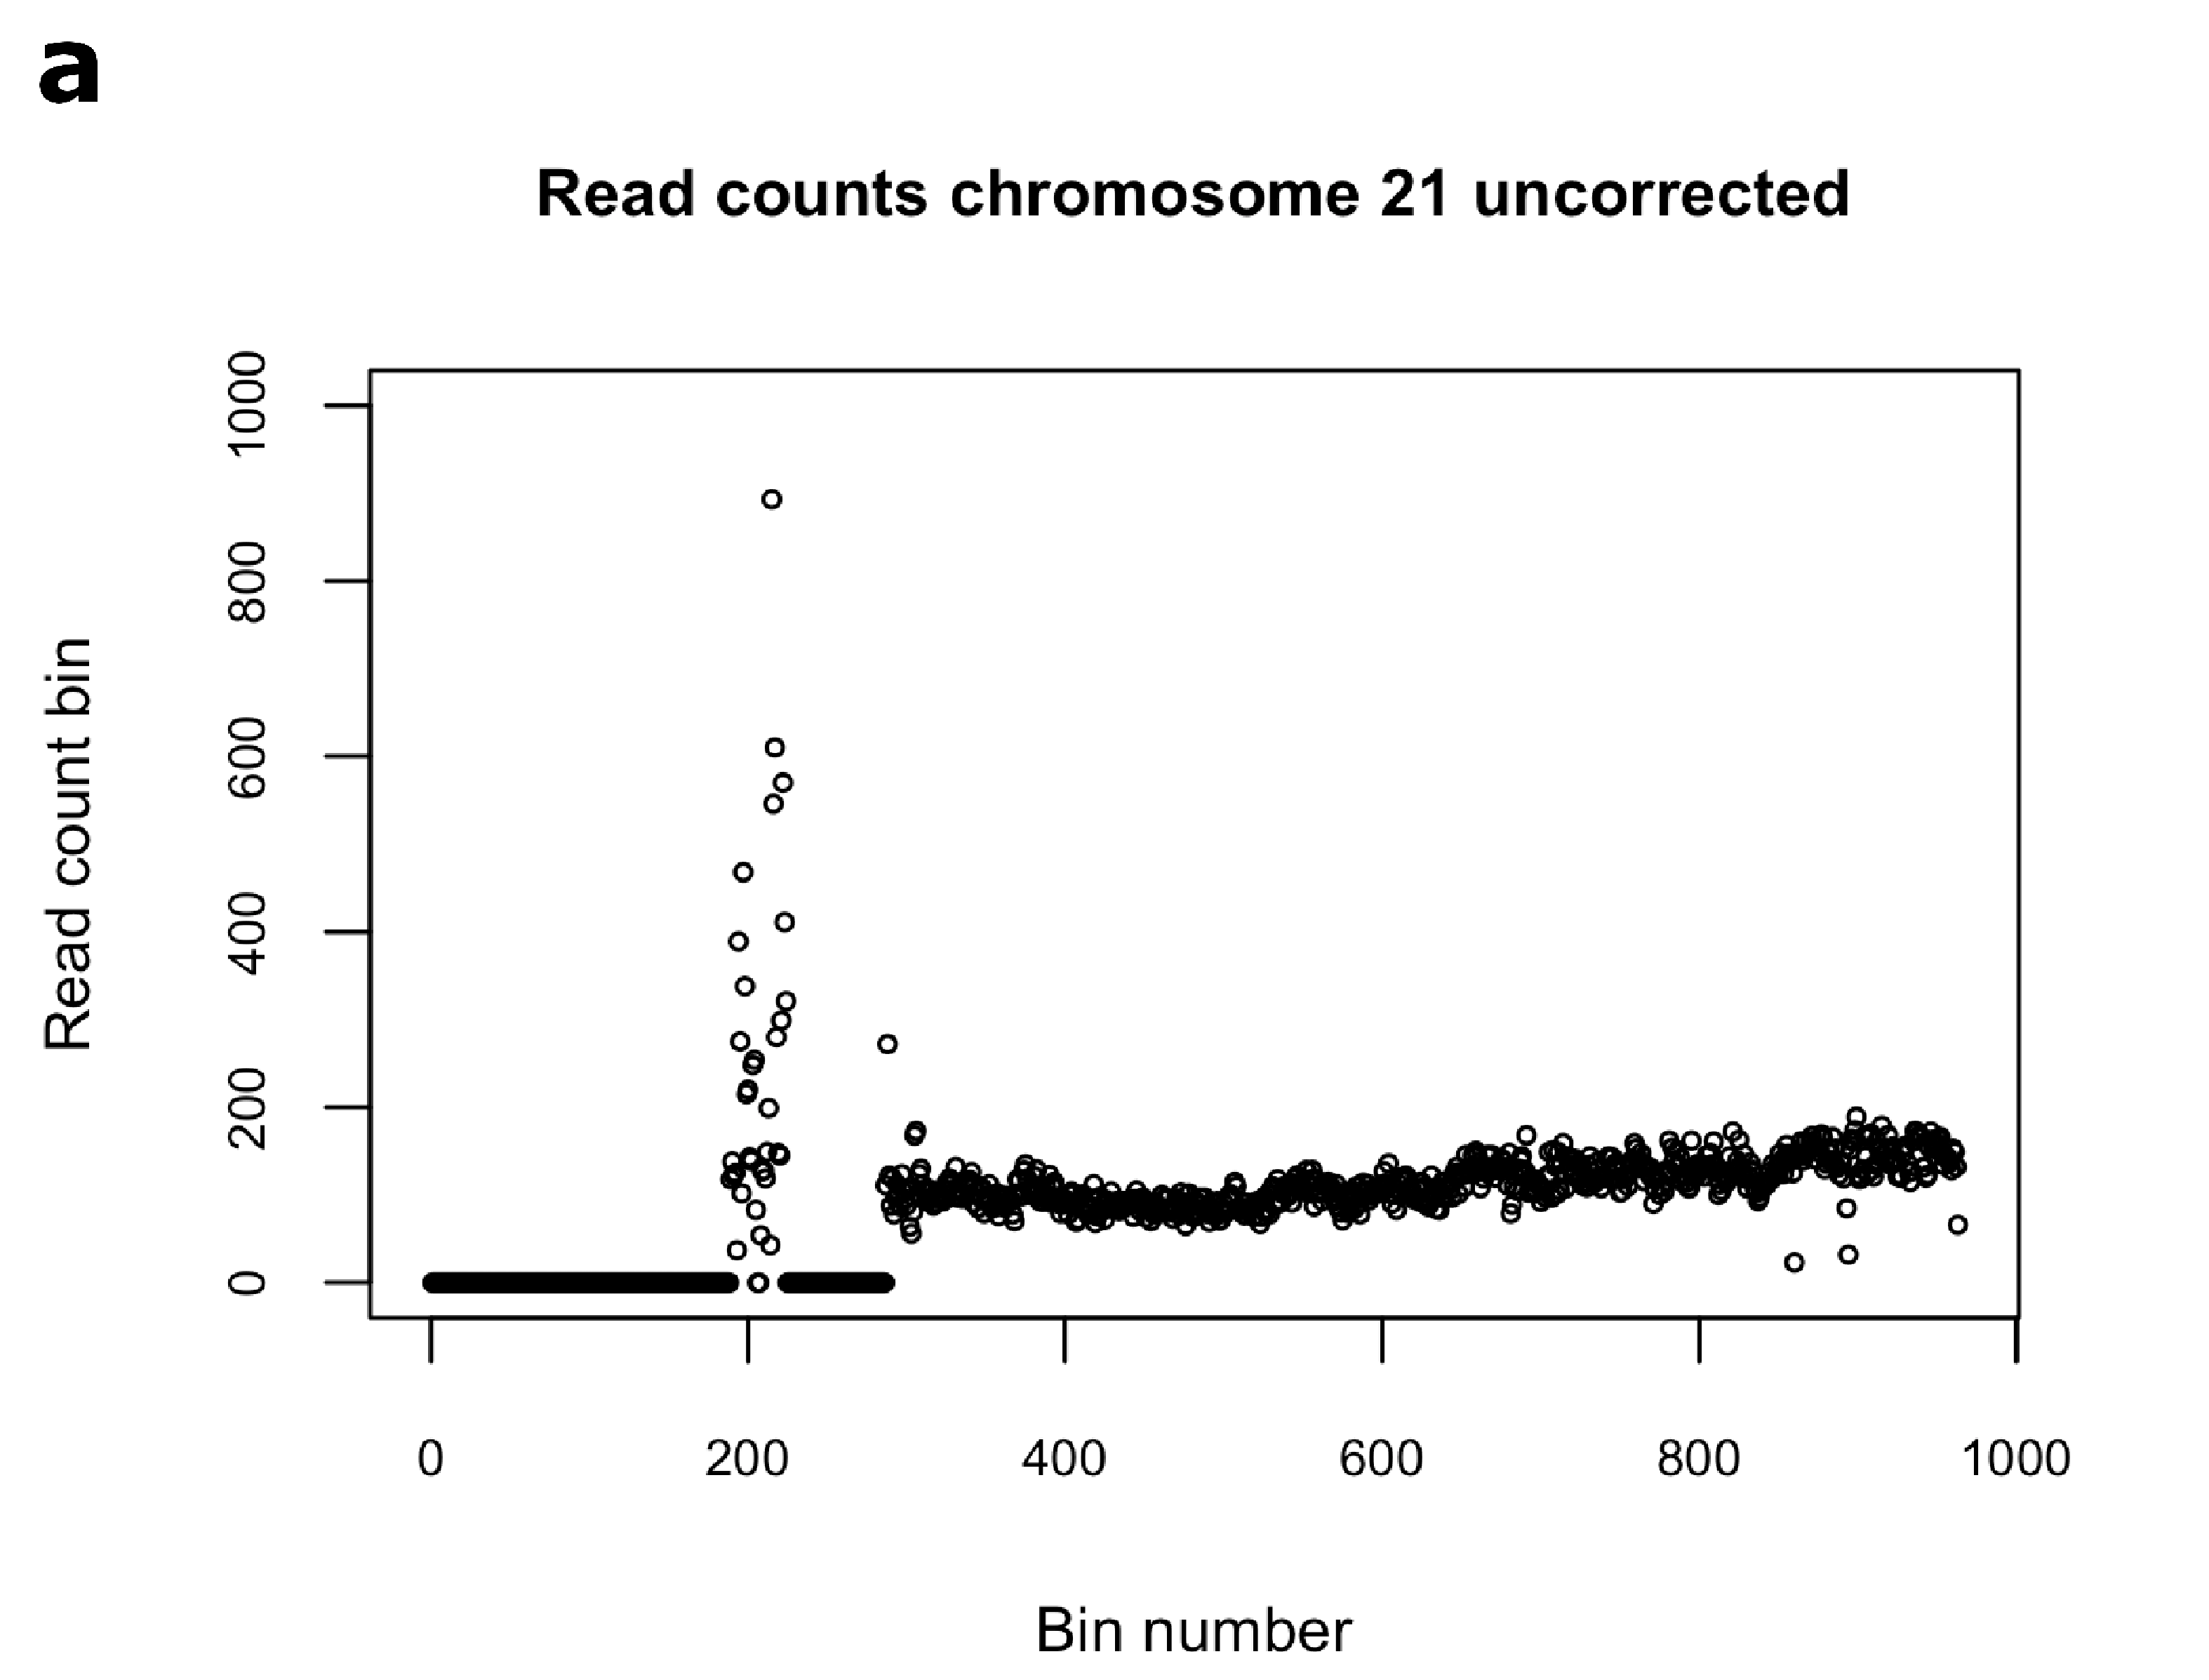
\includegraphics[width=1\linewidth]{img/NIPT_Supp1_Fig1_1a}
		\label{fig:NIPT_Supp1_Fig1_1a}
	\end{subfigure}%
	\begin{subfigure}{.5\textwidth}
		\centering
		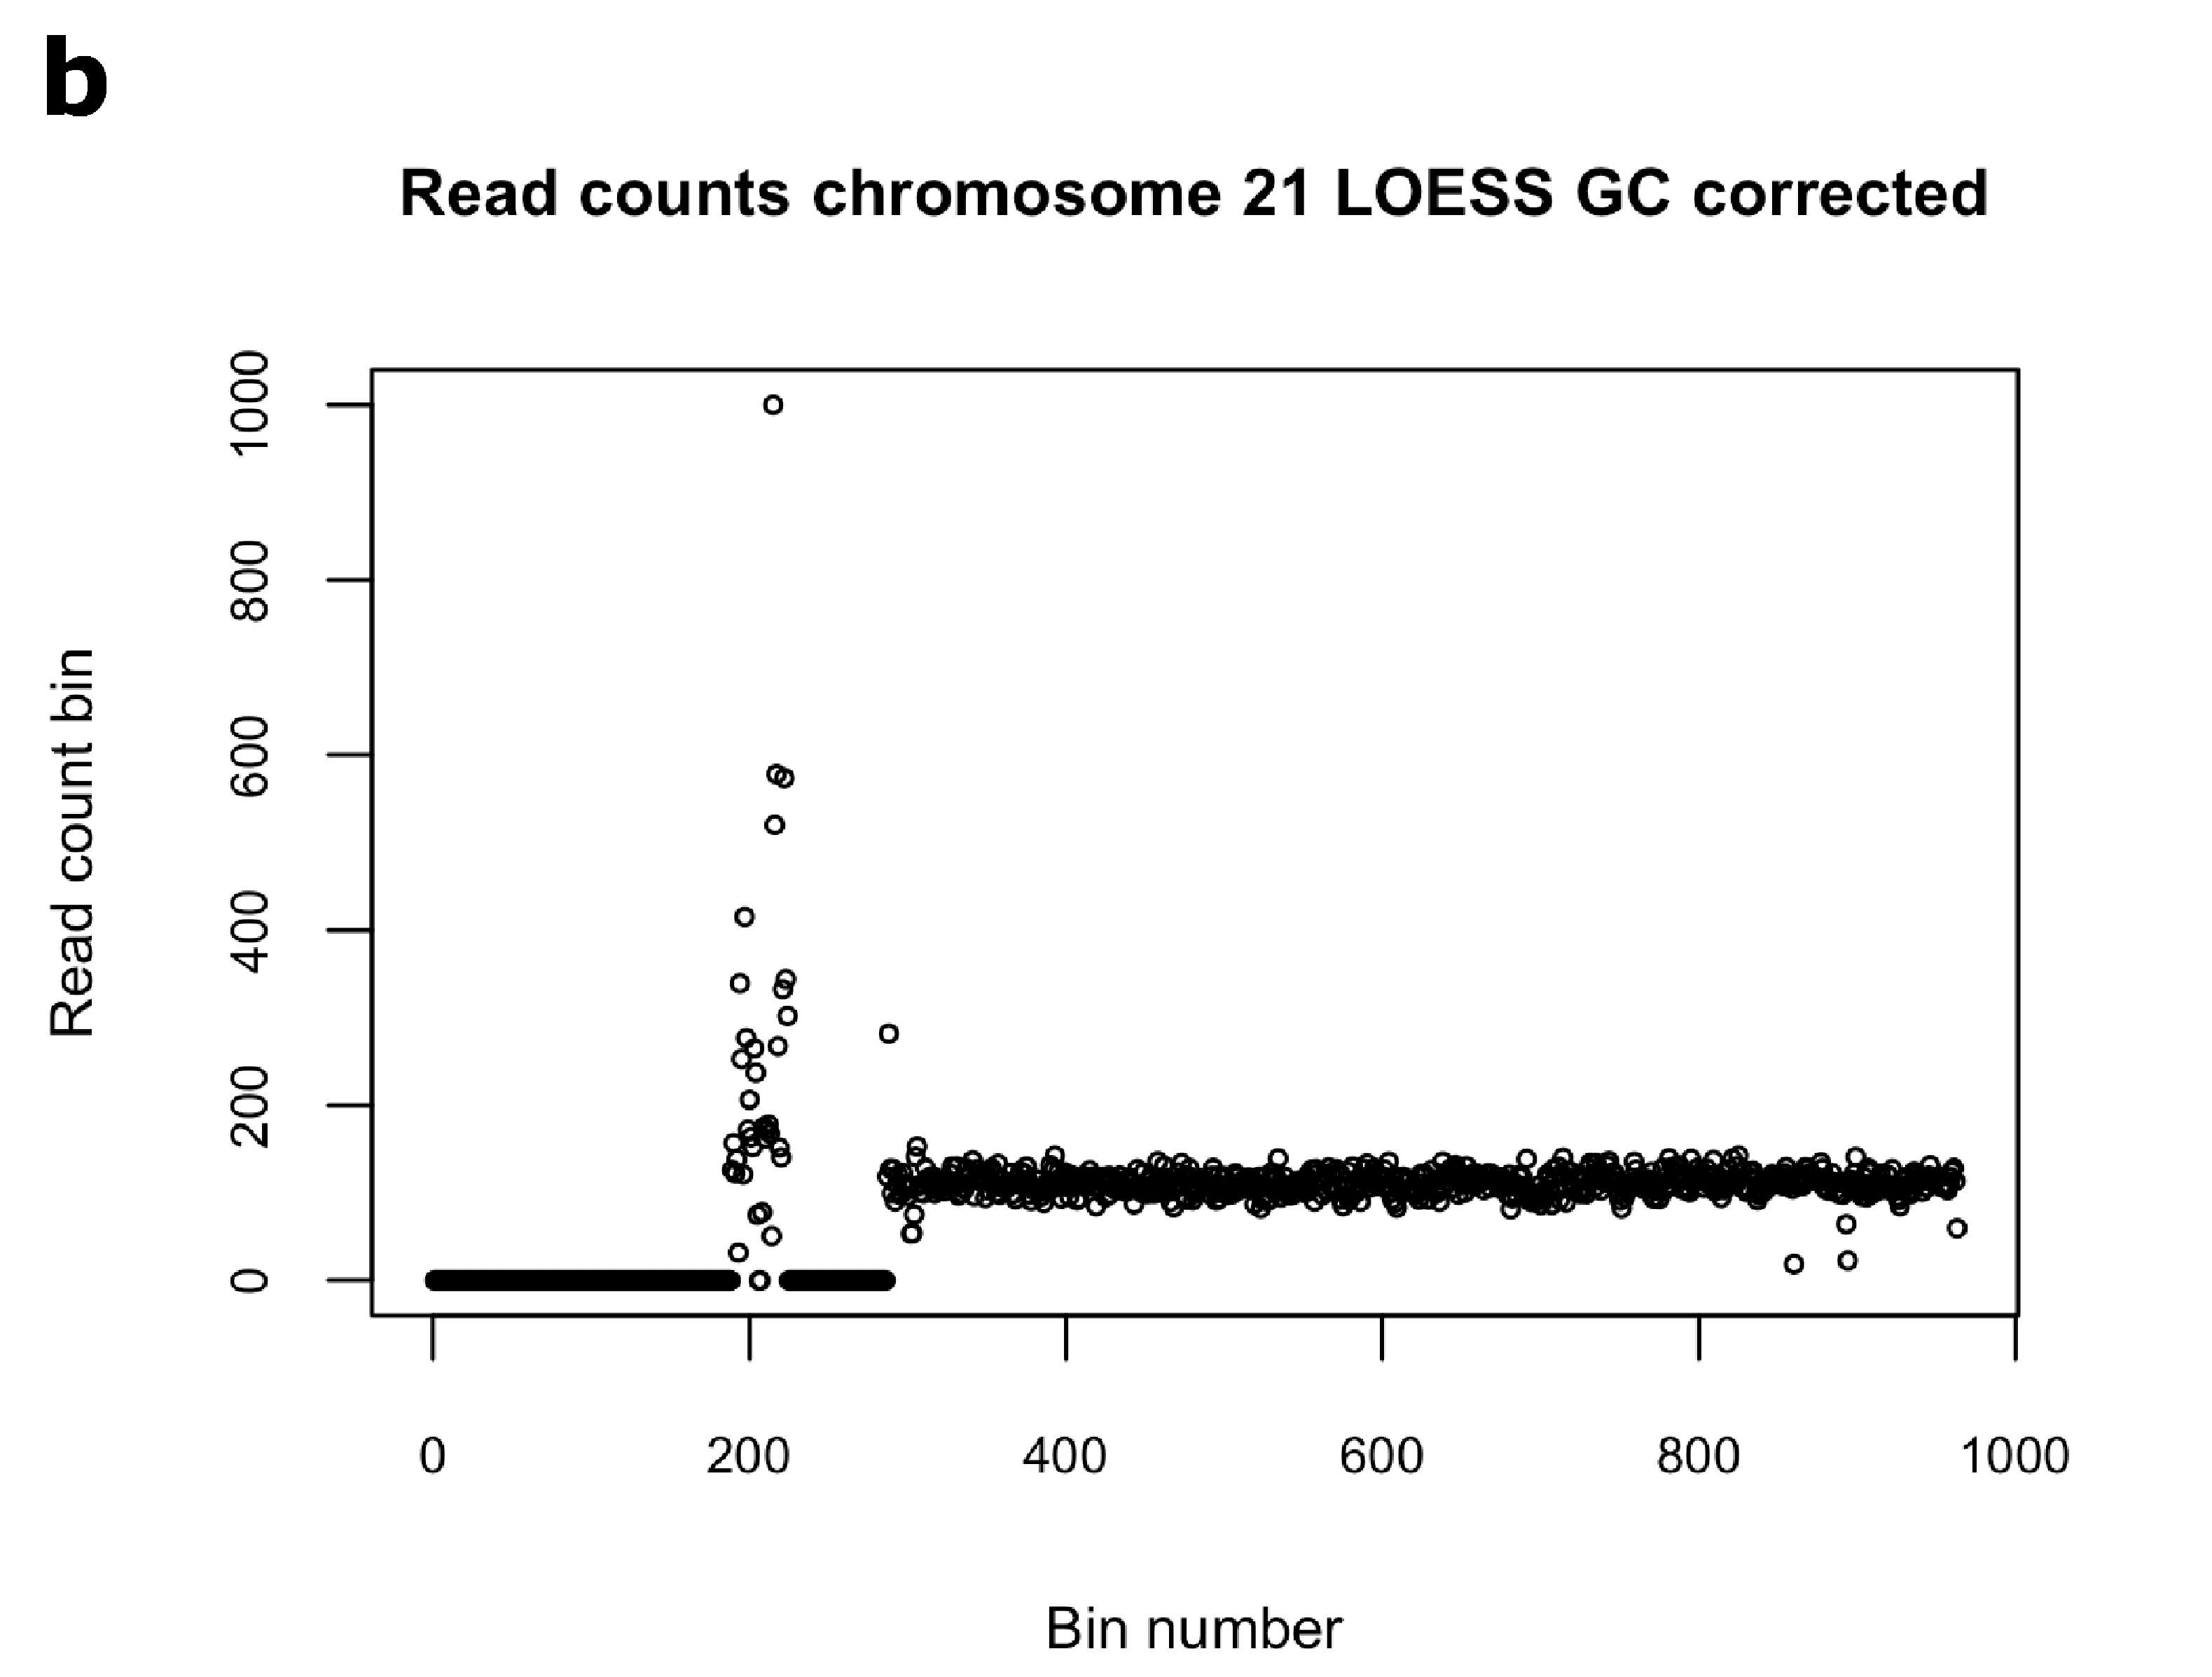
\includegraphics[width=1\linewidth]{img/NIPT_Supp1_Fig1_1b}
		\label{fig:NIPT_Supp1_Fig1_1b}
	\end{subfigure} 
	\caption[Example effect $\chi$\textsuperscript{2}VR on bin counts]{\textbf{Read counts bins chromosome 21 without $\chi$\textsuperscript{2}VR of one of the Illumina control group samples} \textbf{(a)} uncorrected data. \textbf{(b)}LOESS GC corrected data.}
	\label{fig:NIPT_Supp1_Fig1_1}
\end{figure}

\begin{figure}[!hb]
	\begin{subfigure}{.5\textwidth}
		\centering
		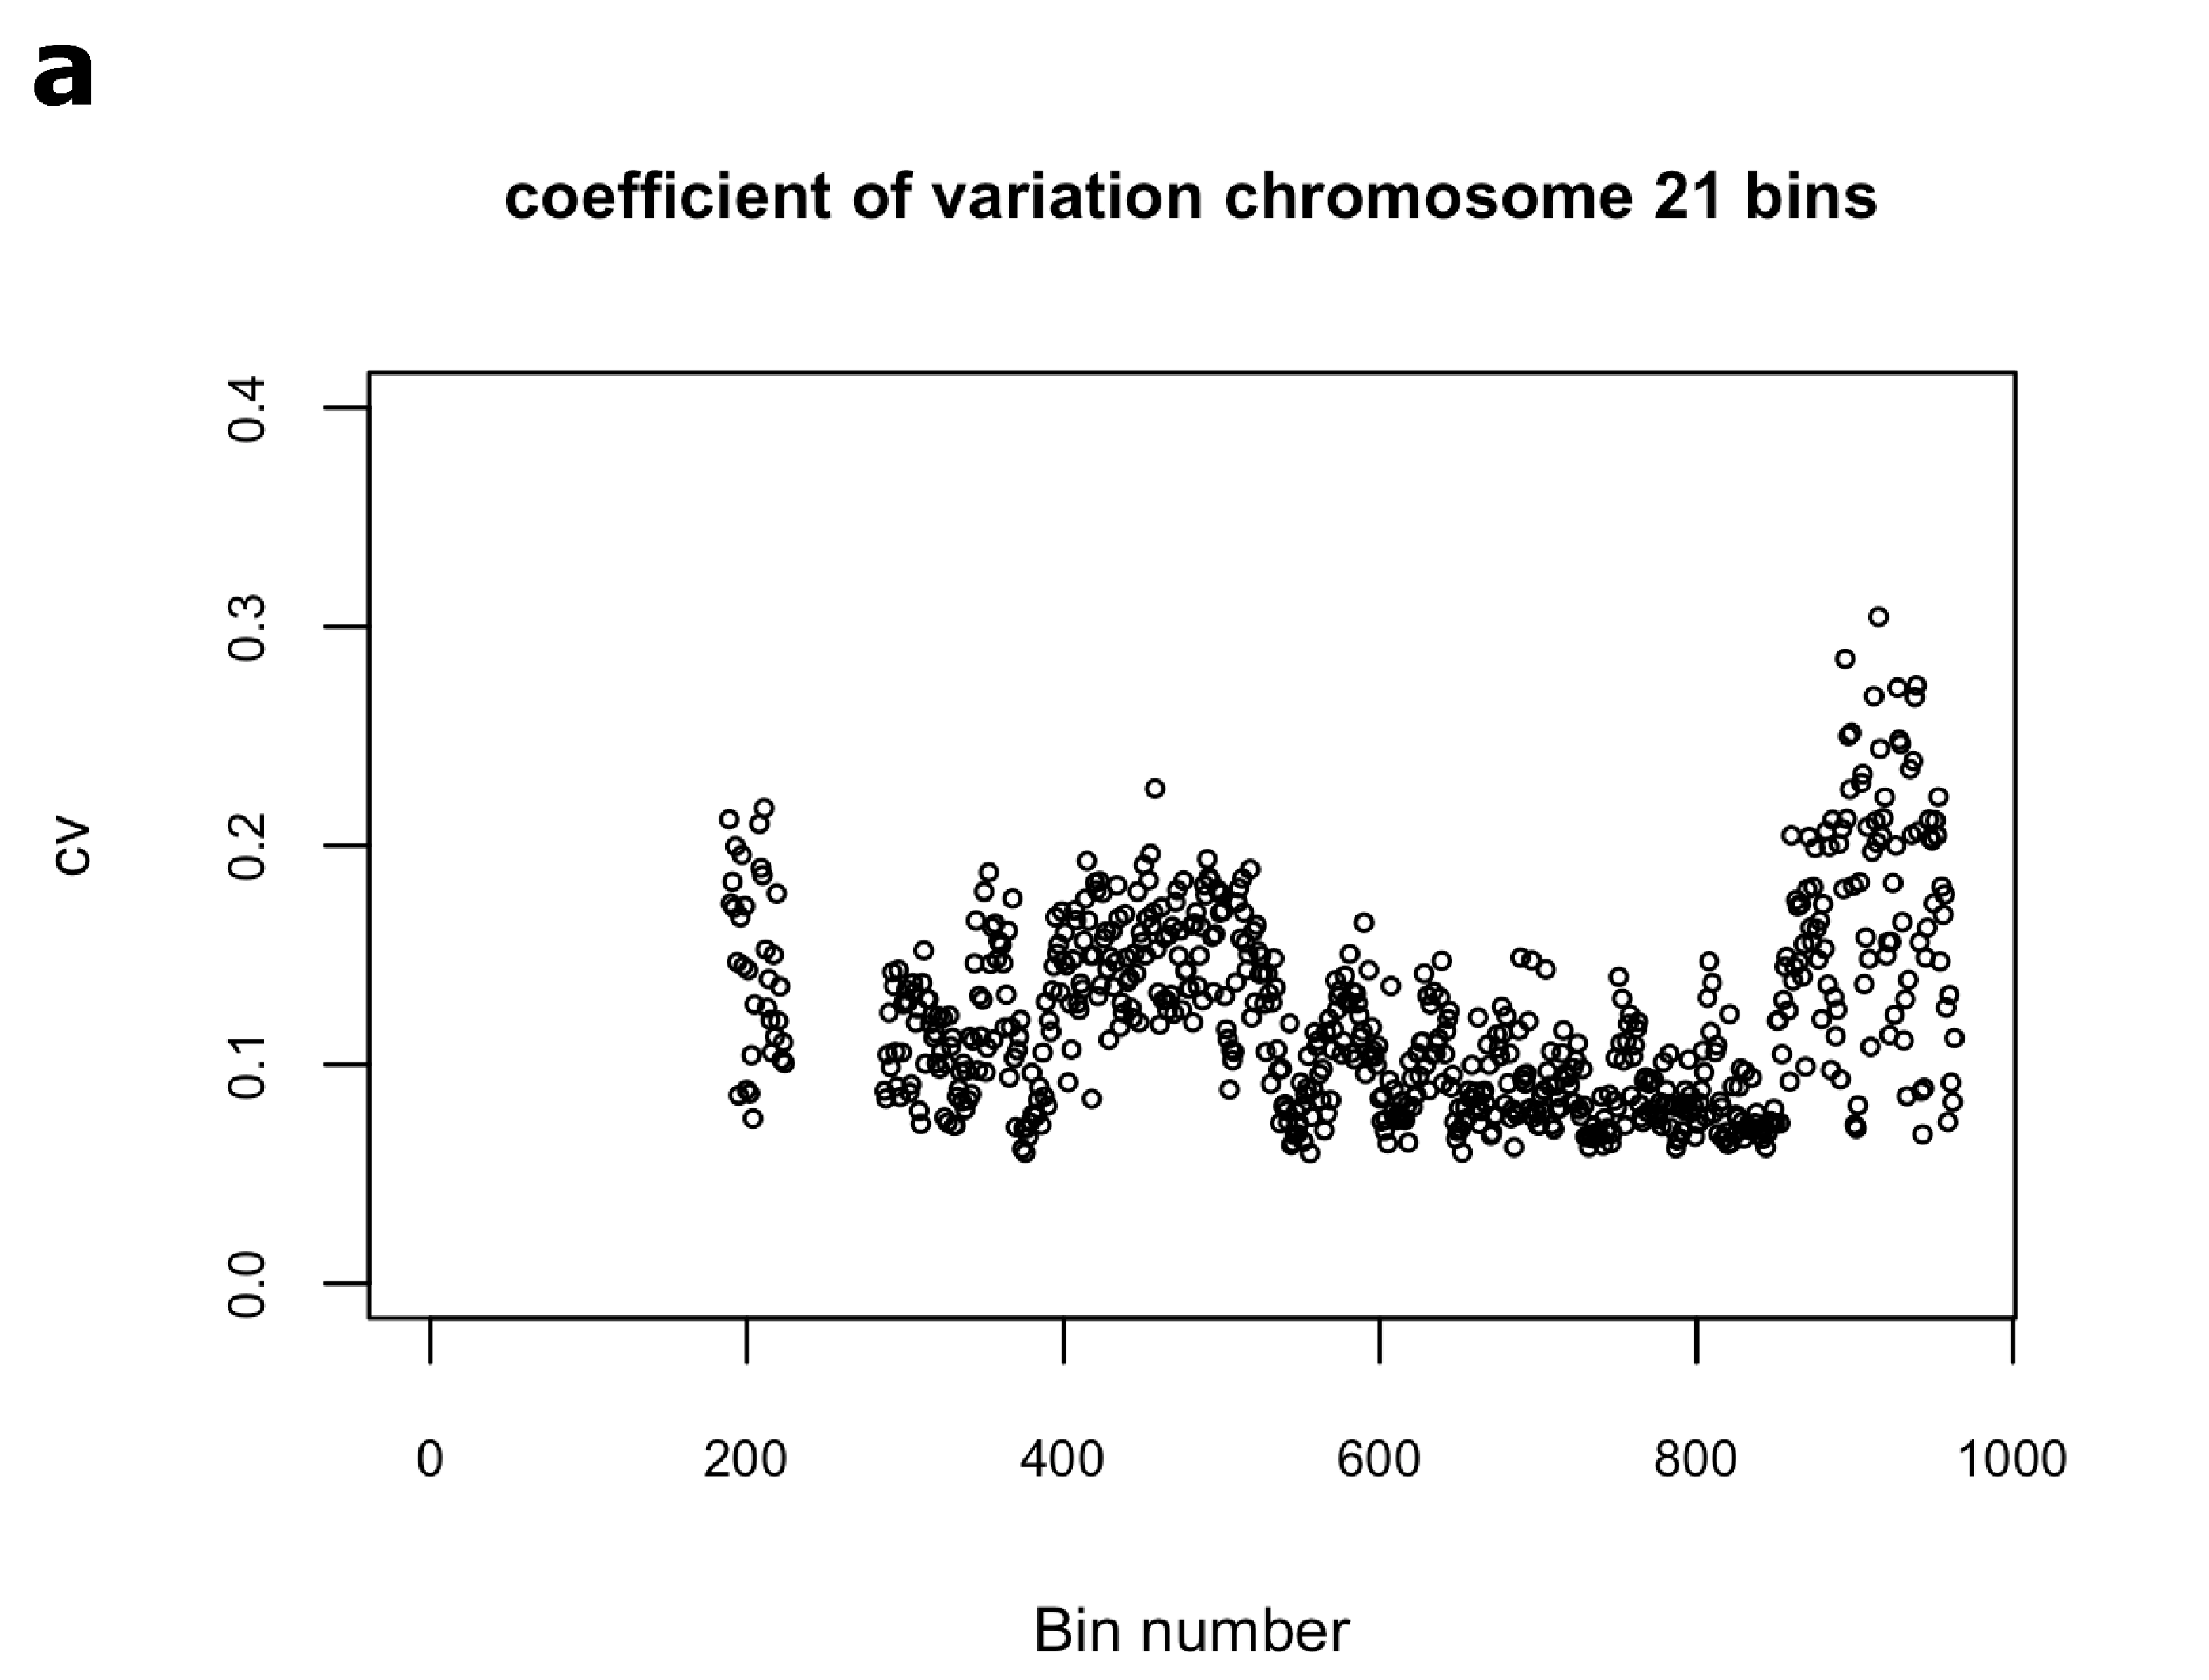
\includegraphics[width=1\linewidth]{img/NIPT_Supp1_Fig1_2a}
		\label{fig:NIPT_Supp1_Fig1_2a}
	\end{subfigure}%
	\begin{subfigure}{.5\textwidth}
		\centering
		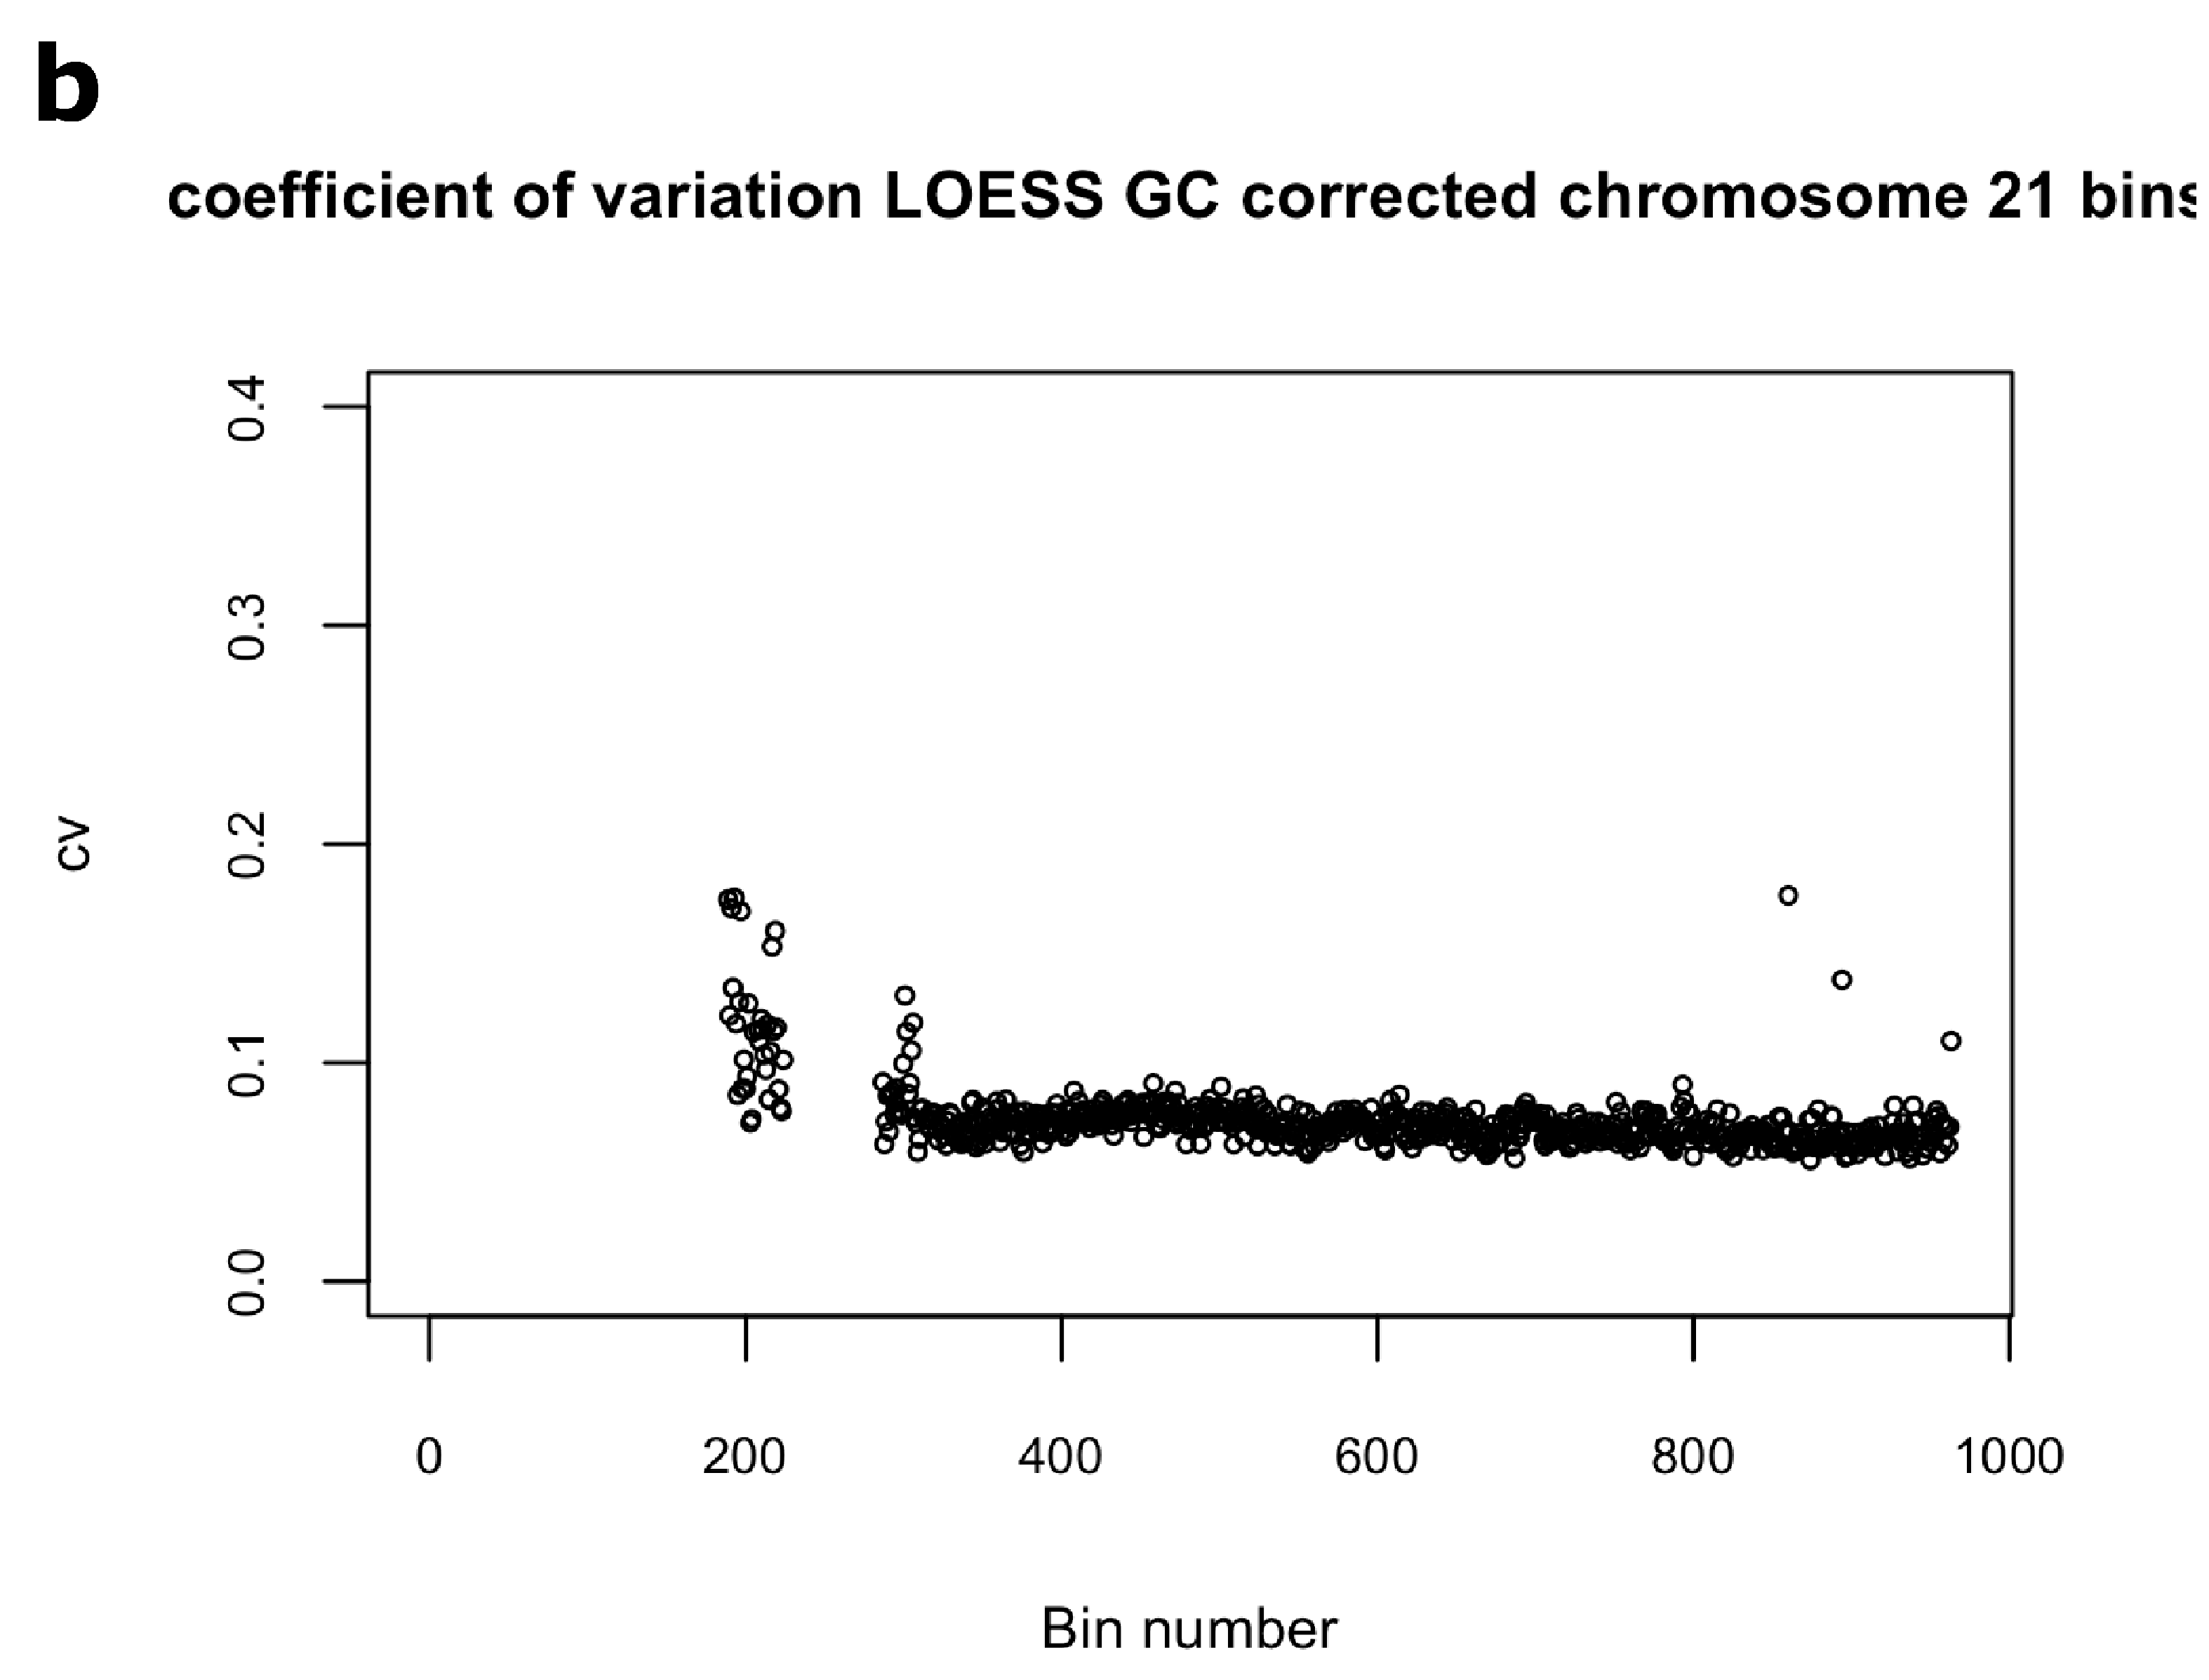
\includegraphics[width=1\linewidth]{img/NIPT_Supp1_Fig1_2b}
		\label{fig:NIPT_Supp1_Fig1_2b}
	\end{subfigure} 
	\caption[Example CV per bin with and without $\chi$\textsuperscript{2}VR]{\textbf{Coefficient of variation bins chromosome 21 without $\chi$\textsuperscript{2}VR of the Illumina control group samples} \textbf{(a)} uncorrected data. \textbf{(b)} LOESS GC corrected data.}
	\label{fig:NIPT_Supp1_Fig1_2}
\end{figure}

\noindent The input of the $\chi$\textsuperscript{2}VR are sample and control group, bin-counts of uncorrected data or data corrected using different variation reduction methods, such as GC correction (Fig. \ref{fig:NIPT_Supp1_Fig1_1}). 
The examples are based upon the 142 Illumina control samples. 
In some images read counts of a single sample are shown. For these images a random sample was selected from the control group.

\begin{figure}[!h]
	\begin{subfigure}{.5\textwidth}
		\centering
		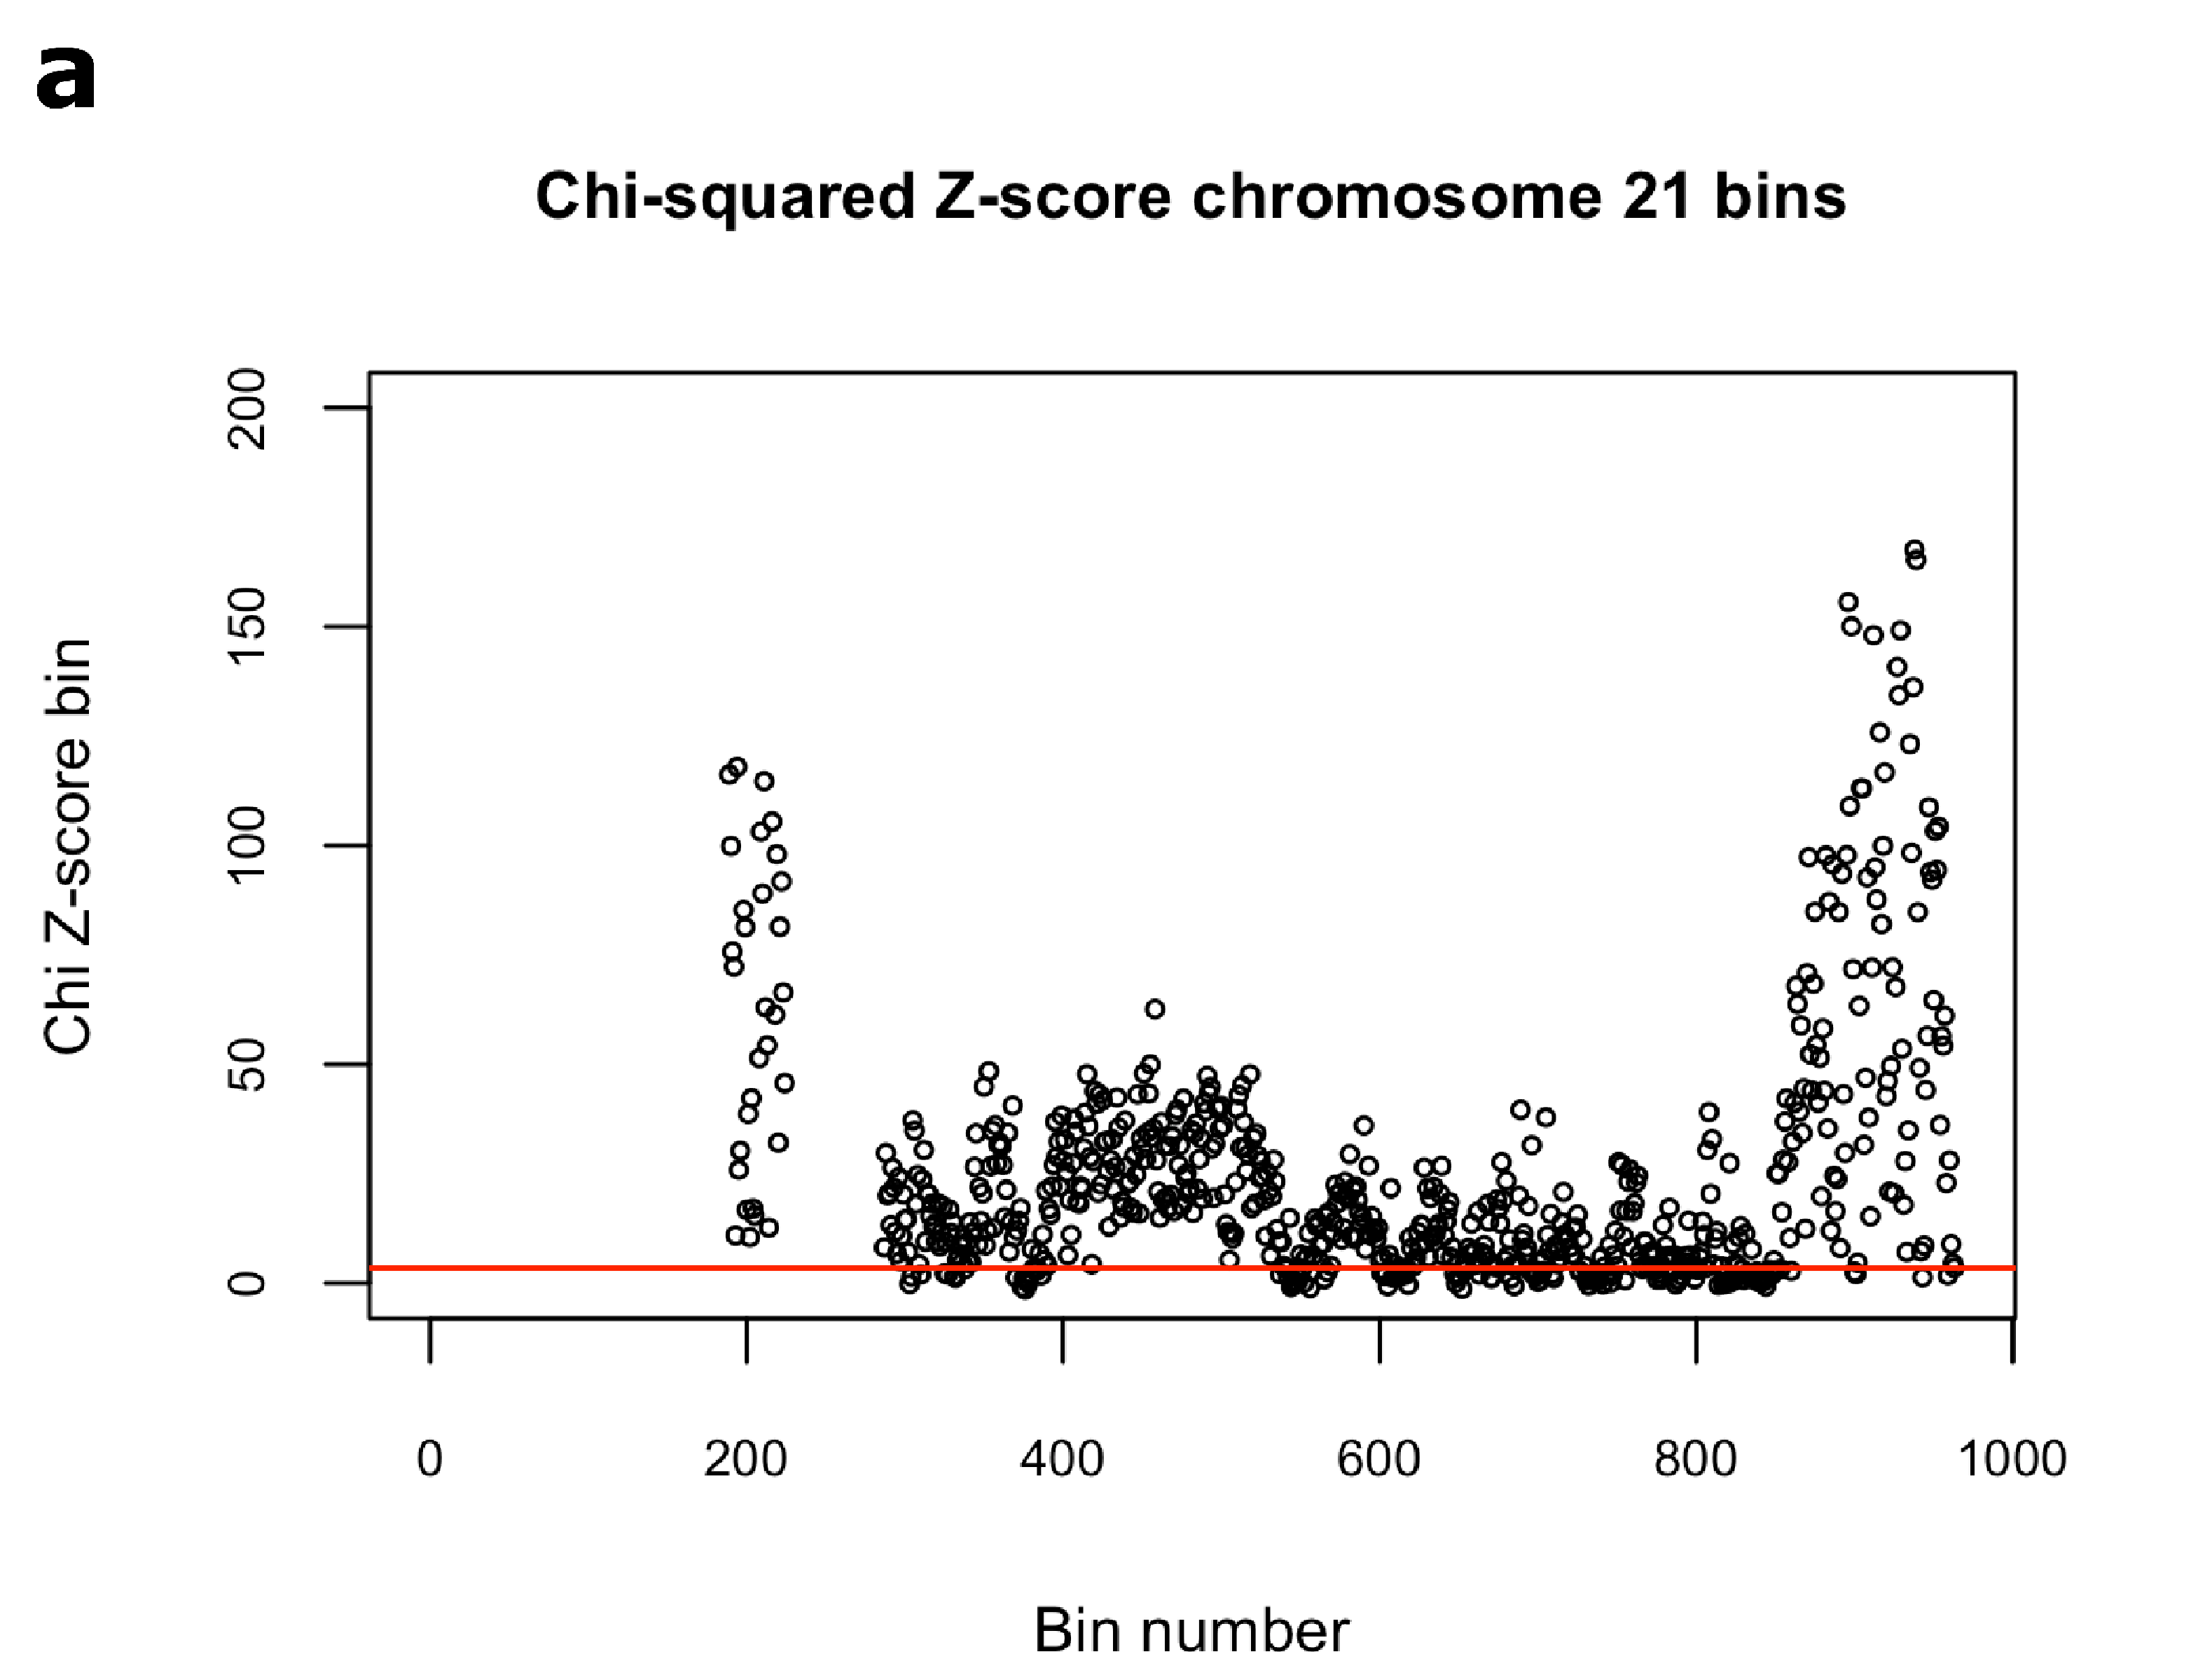
\includegraphics[width=1\linewidth]{img/NIPT_Supp1_Fig1_3a}
		\label{fig:NIPT_Supp1_Fig1_3a}
	\end{subfigure}%
	\begin{subfigure}{.5\textwidth}
		\centering
		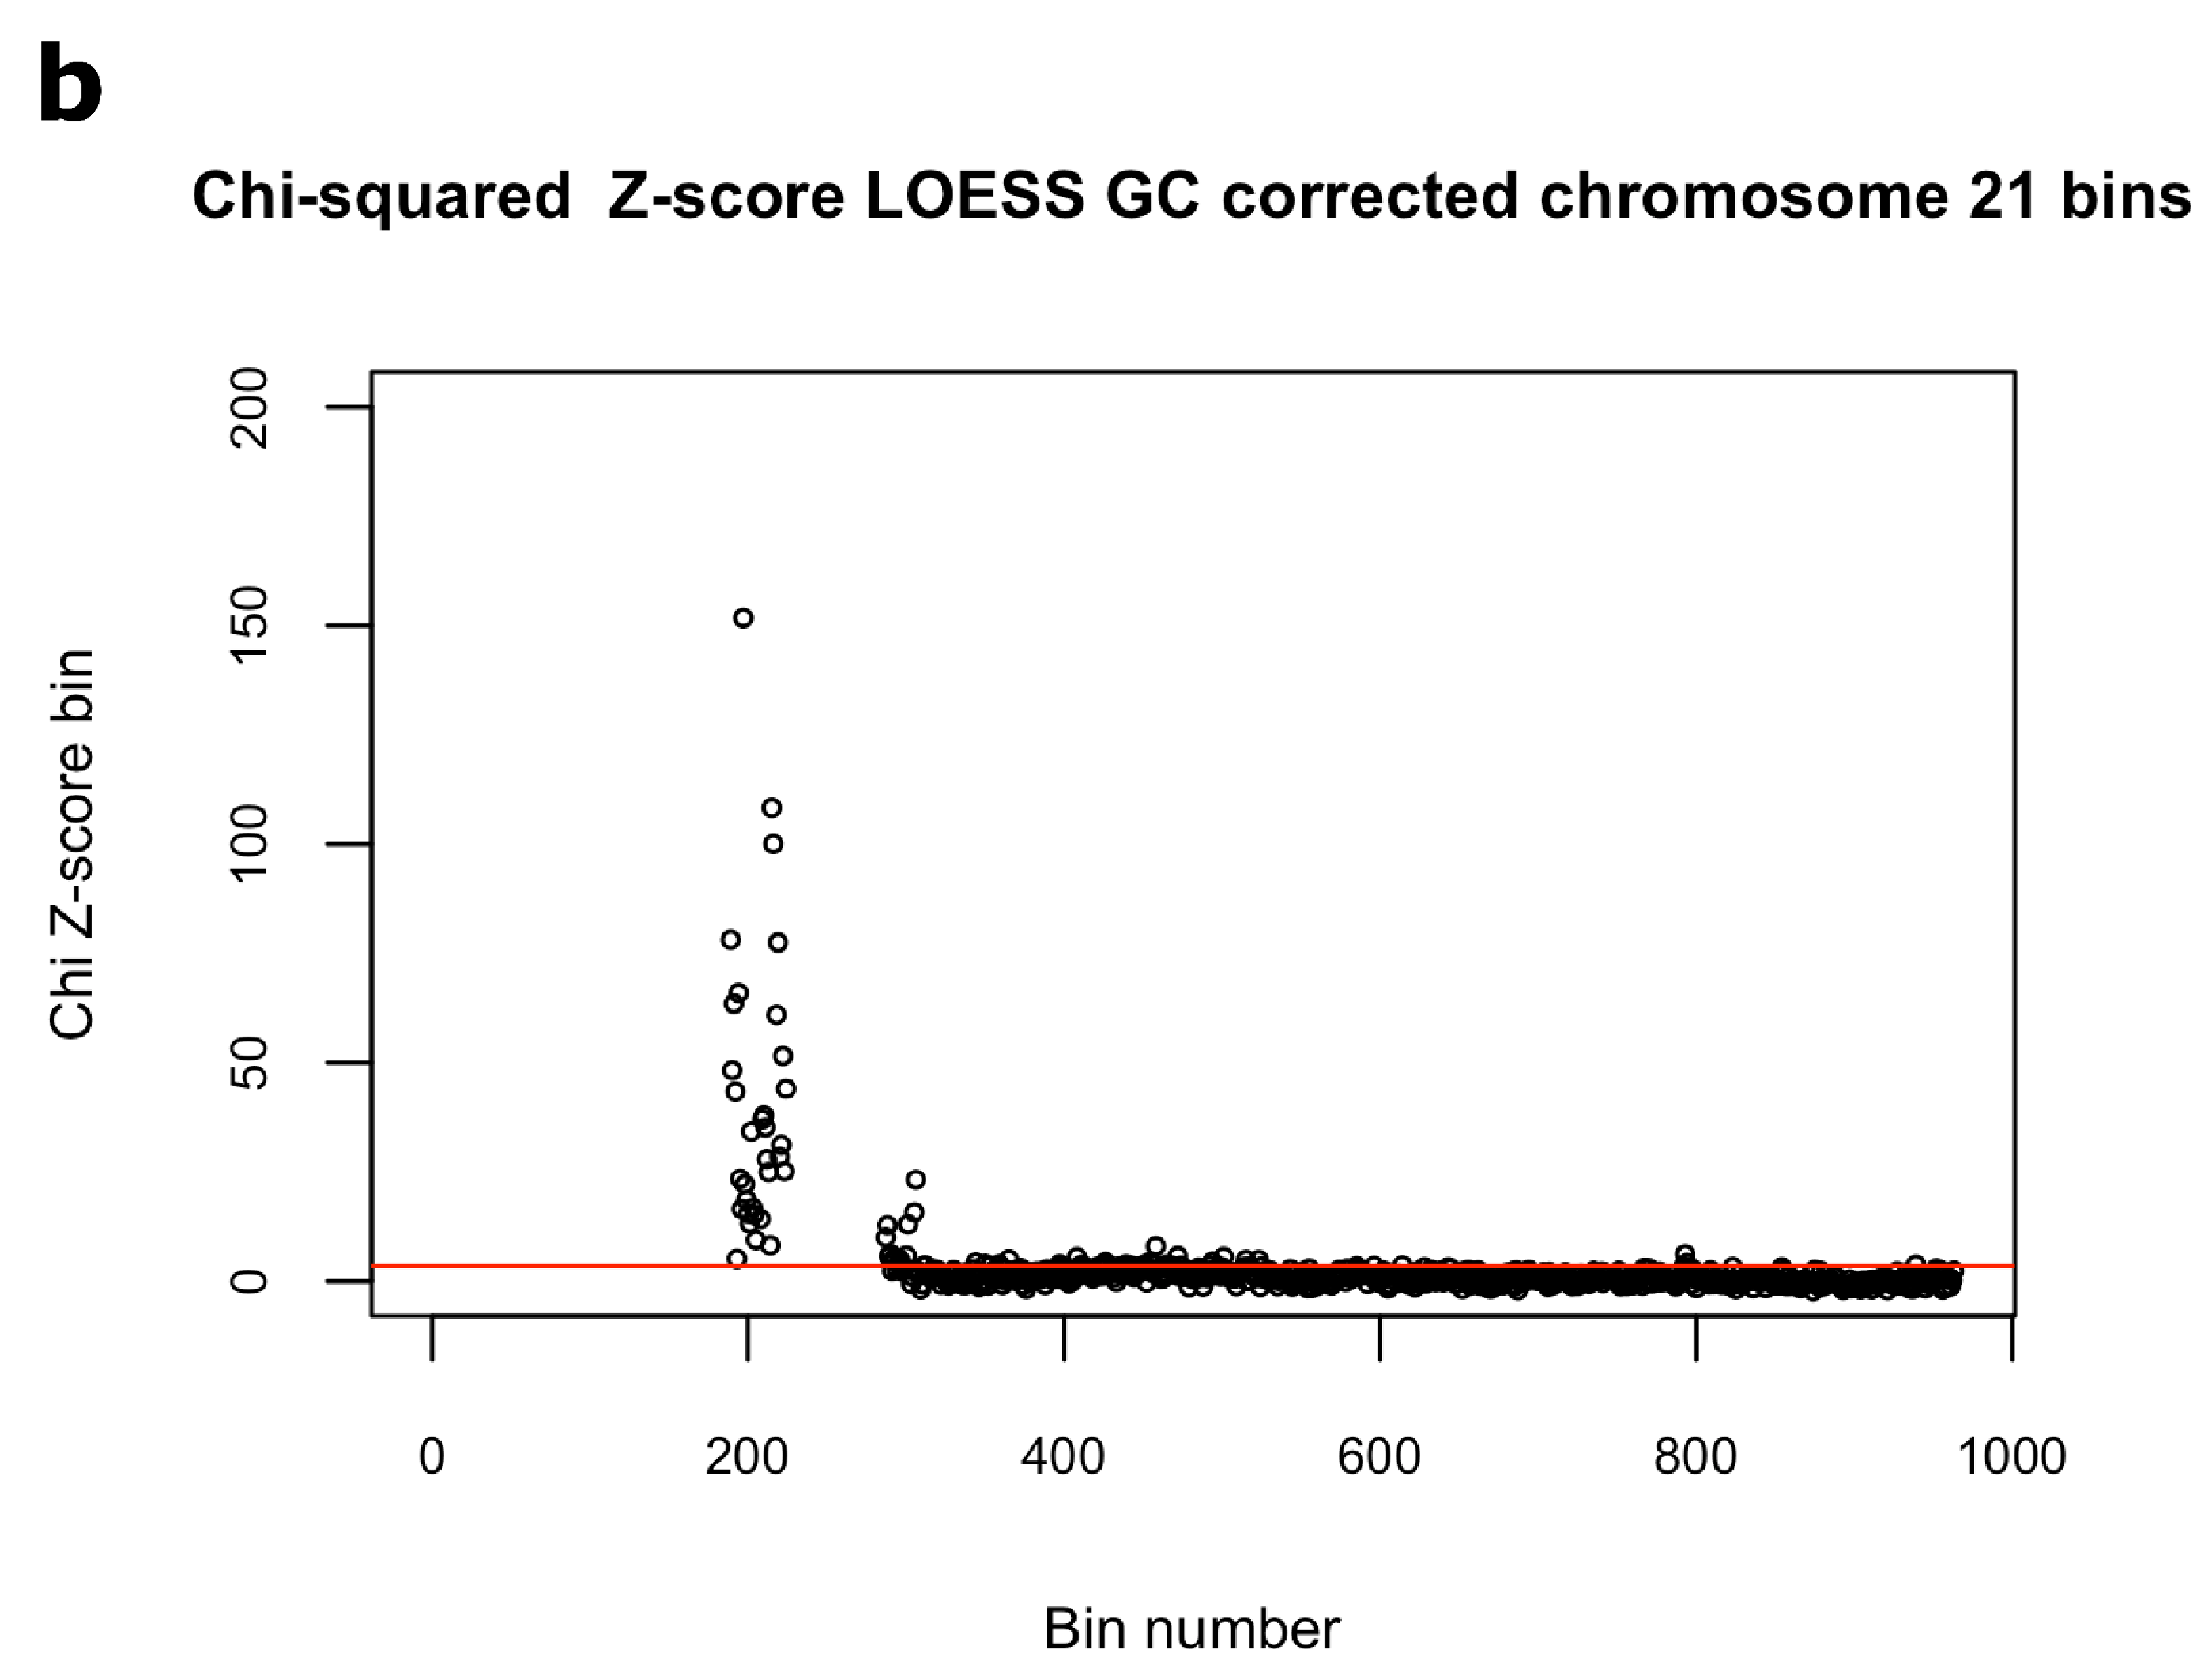
\includegraphics[width=1\linewidth]{img/NIPT_Supp1_Fig1_3b}
		\label{fig:NIPT_Supp1_Fig1_3b}
	\end{subfigure}
	\begin{subfigure}{.5\textwidth}
		\centering
		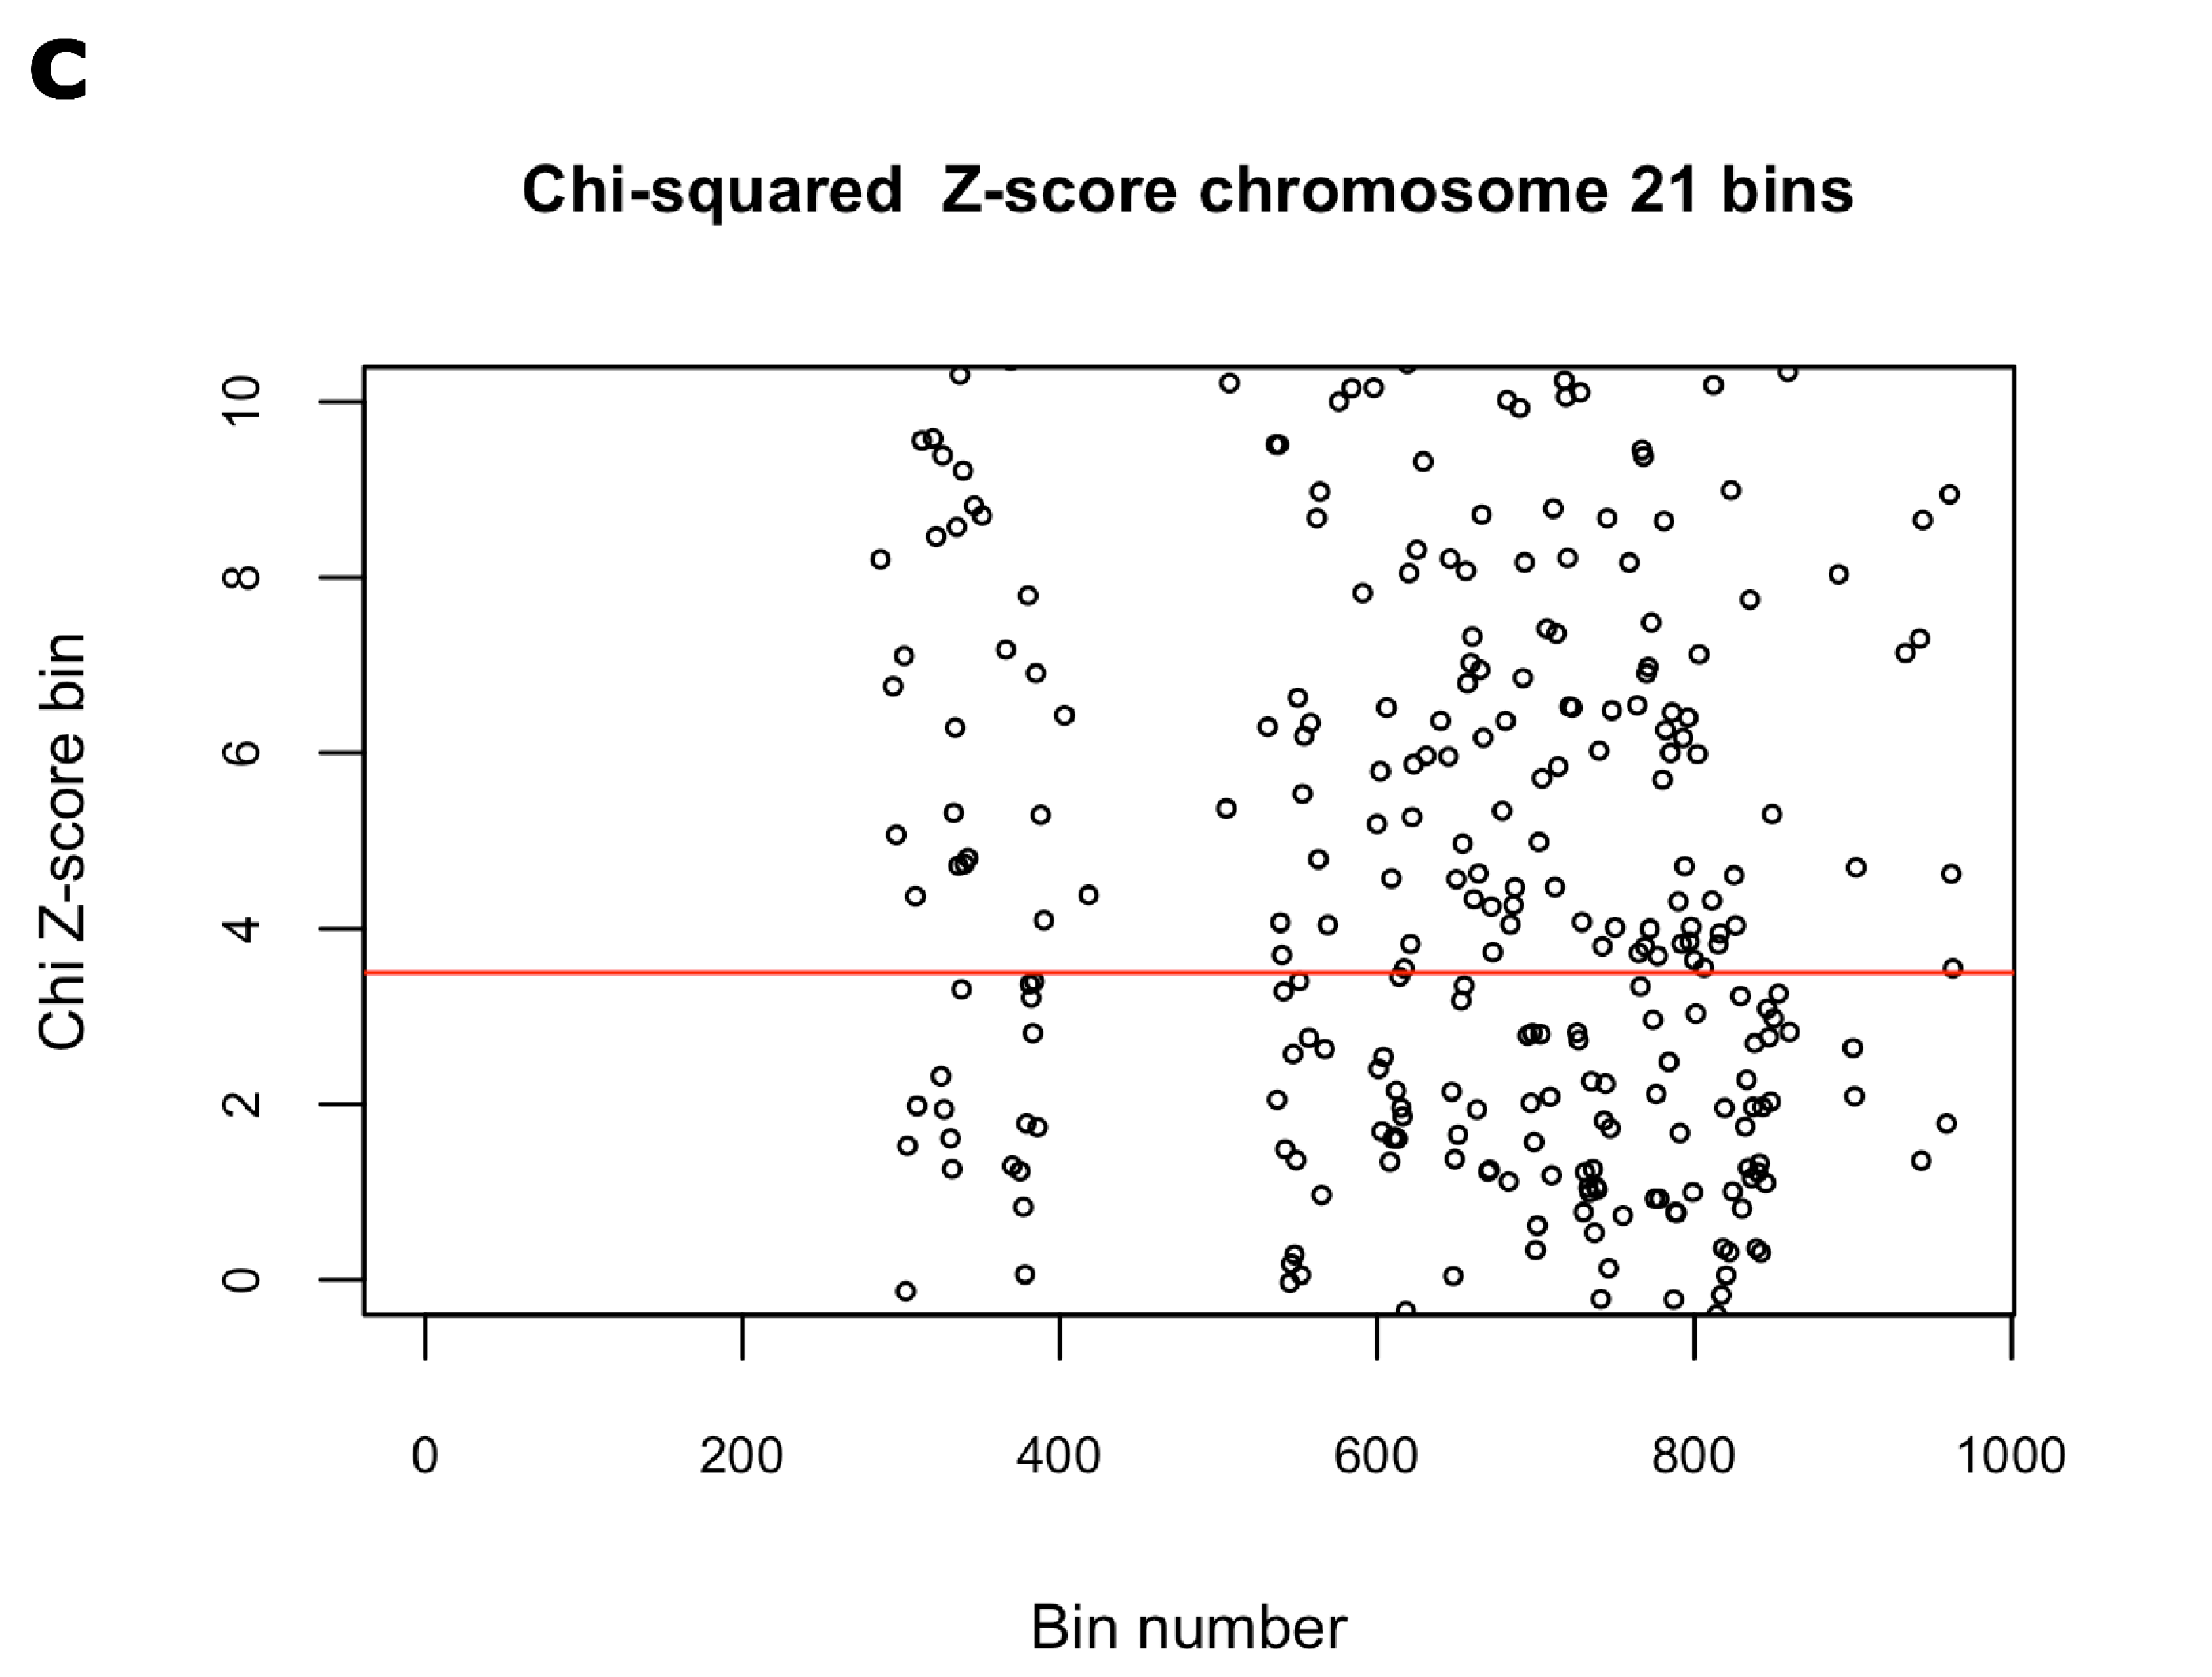
\includegraphics[width=1\linewidth]{img/NIPT_Supp1_Fig1_3c}
		\label{fig:NIPT_Supp1_Fig1_3c}
	\end{subfigure} 
	\begin{subfigure}{.5\textwidth}
		\centering
		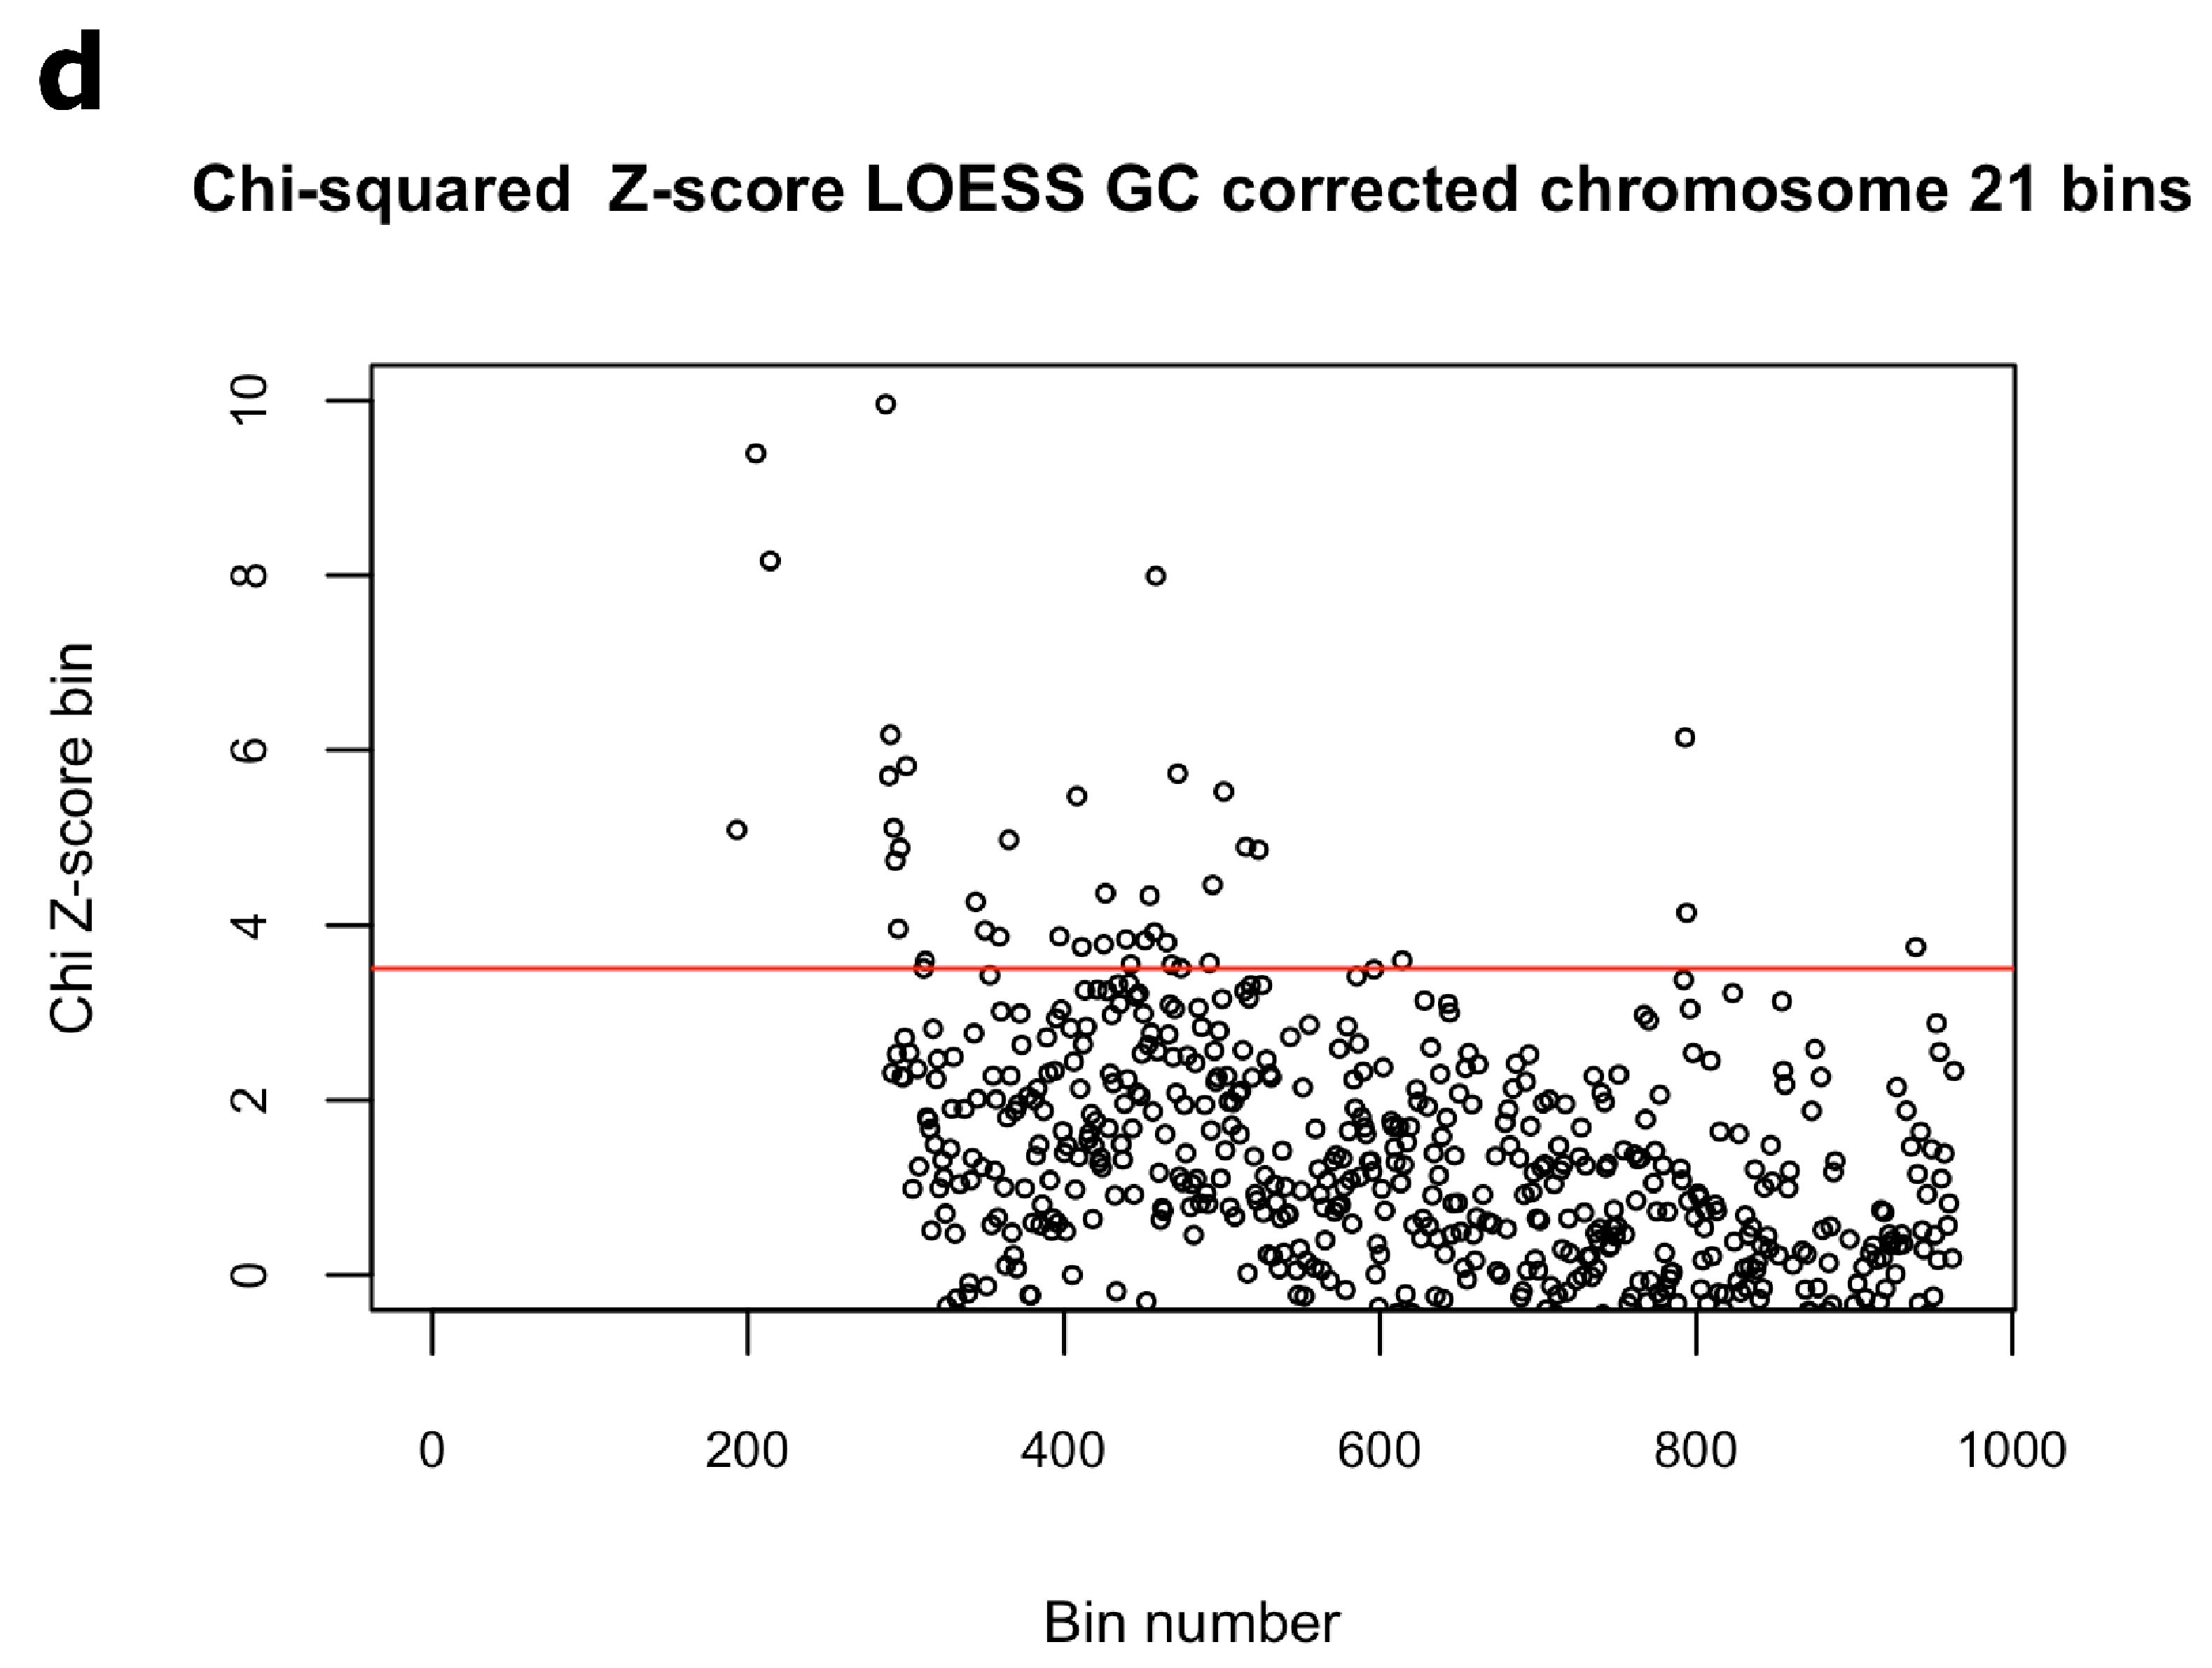
\includegraphics[width=1\linewidth]{img/NIPT_Supp1_Fig1_3d}
		\label{fig:NIPT_Supp1_Fig1_3d}
	\end{subfigure}  
	\caption[Example Z-score normal distribution sum chi-squared value]{\textbf{Z-score sum chi-squared value after transformation to normal distribution for all bins chromosome 21 based upon the Illumina control group samples} \textbf{(a)} uncorrected data, total range. \textbf{(b)} LOESS GC corrected data, total range. \textbf{(c)} uncorrected data, plotted until a maximum Z-score of 10. \textbf{(d)} LOESS GC corrected data, pltoted until a maximum Z-score of 10.}
	\label{fig:NIPT_Supp1_Fig1_3}
\end{figure}

\noindent First the data is normalized by dividing the mean read count of the bin by the mean read count of all autosomal bins. 
After this normalization sample read counts can be compared. 
In some of the bins the normalized read count is consistent between samples, resulting in a low coefficient of variation (CV). 
Other bins have a higher variability between samples, resulting in a higher CV (Fig. \ref{fig:NIPT_Supp1_Fig1_2}).
A GC correction can correct part of the variation. However, even after GC correction some bins still show a high variation.
After normalization for each bin the sum chi-squared value is calculated, using the control samples, and transformed to a standard normal distribution, resulting in a Z-score for each bin (Fig. \ref{fig:NIPT_Supp1_Fig1_3}).

\begin{figure}[h]
	\begin{subfigure}{.5\textwidth}
		\centering
		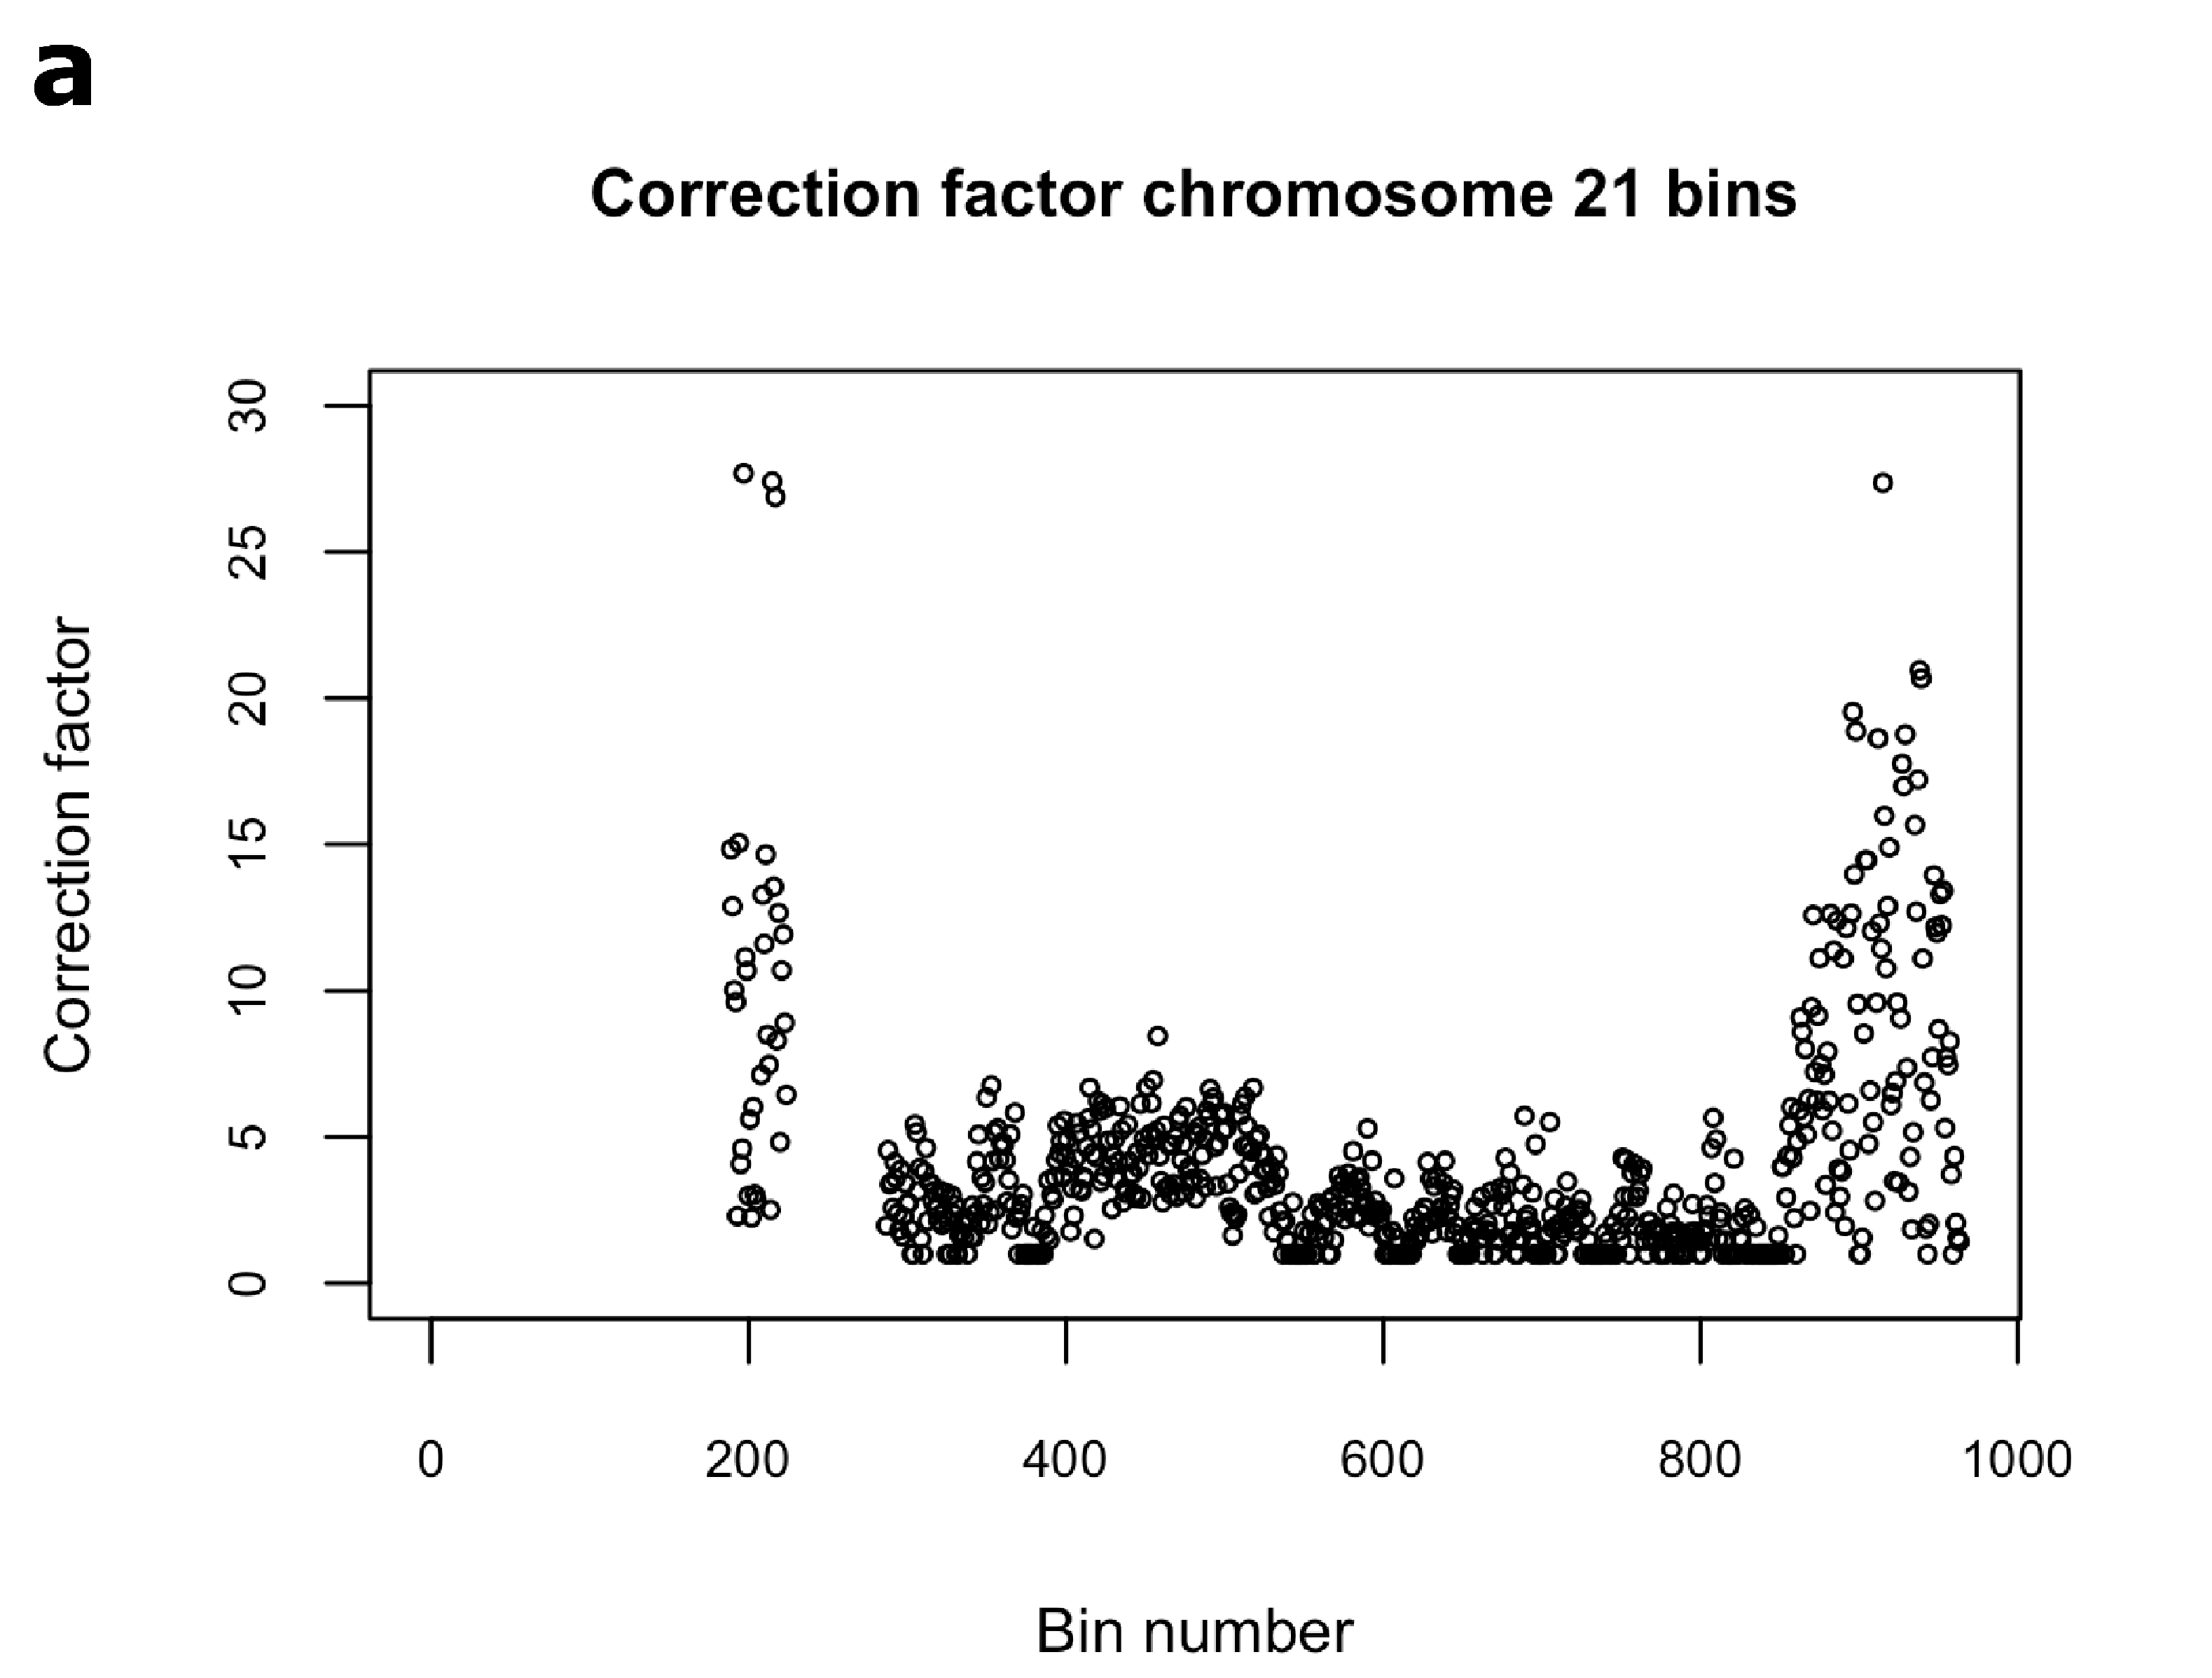
\includegraphics[width=1\linewidth]{img/NIPT_Supp1_Fig1_4a}
		\label{fig:NIPT_Supp1_Fig1_4a}
	\end{subfigure}%
	\begin{subfigure}{.5\textwidth}
		\centering
		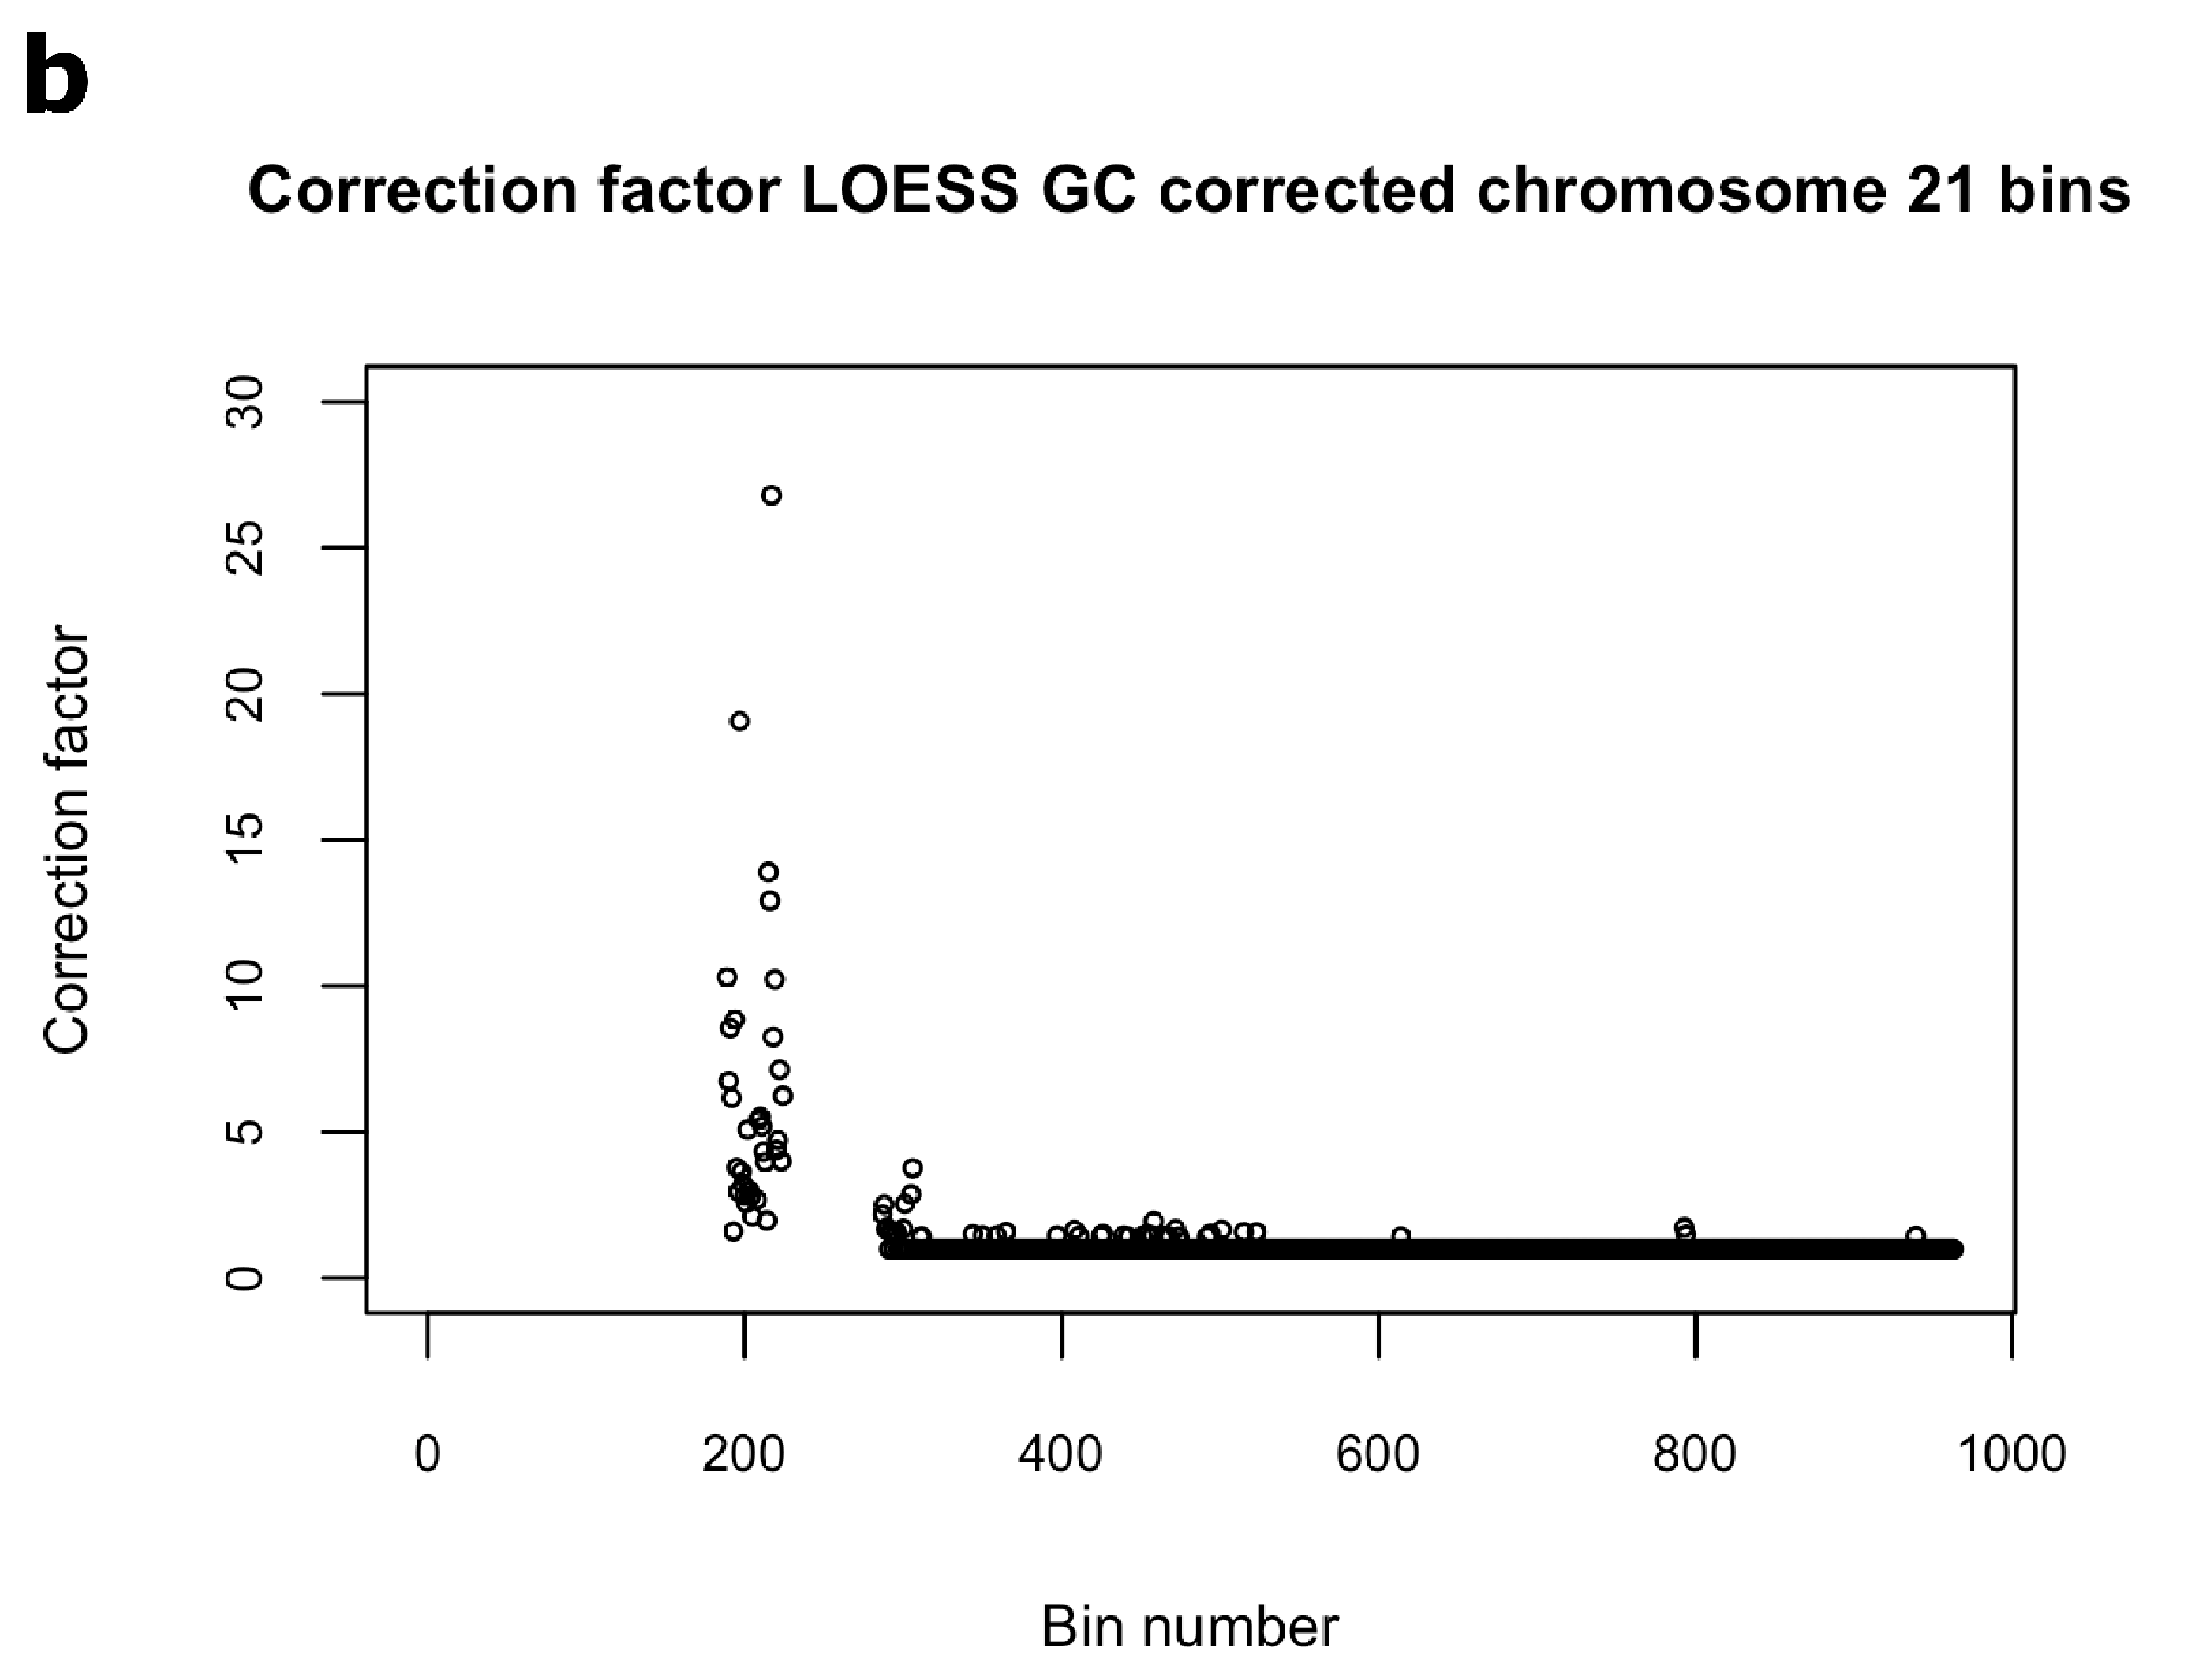
\includegraphics[width=1\linewidth]{img/NIPT_Supp1_Fig1_4b}
		\label{fig:NIPT_Supp1_Fig1_4b}
	\end{subfigure} 
	\caption[Example $\chi$\textsuperscript{2}VR correction factor]{\textbf{$\chi$\textsuperscript{2}VR correction factor bins chromosome 21 based upon Illumina control group} \textbf{(a)} uncorrected data. \textbf{(b)} LOESS GC corrected data.}
	\label{fig:NIPT_Supp1_Fig1_4}
\end{figure}

\begin{figure}[h]
	\begin{subfigure}{.5\textwidth}
		\centering
		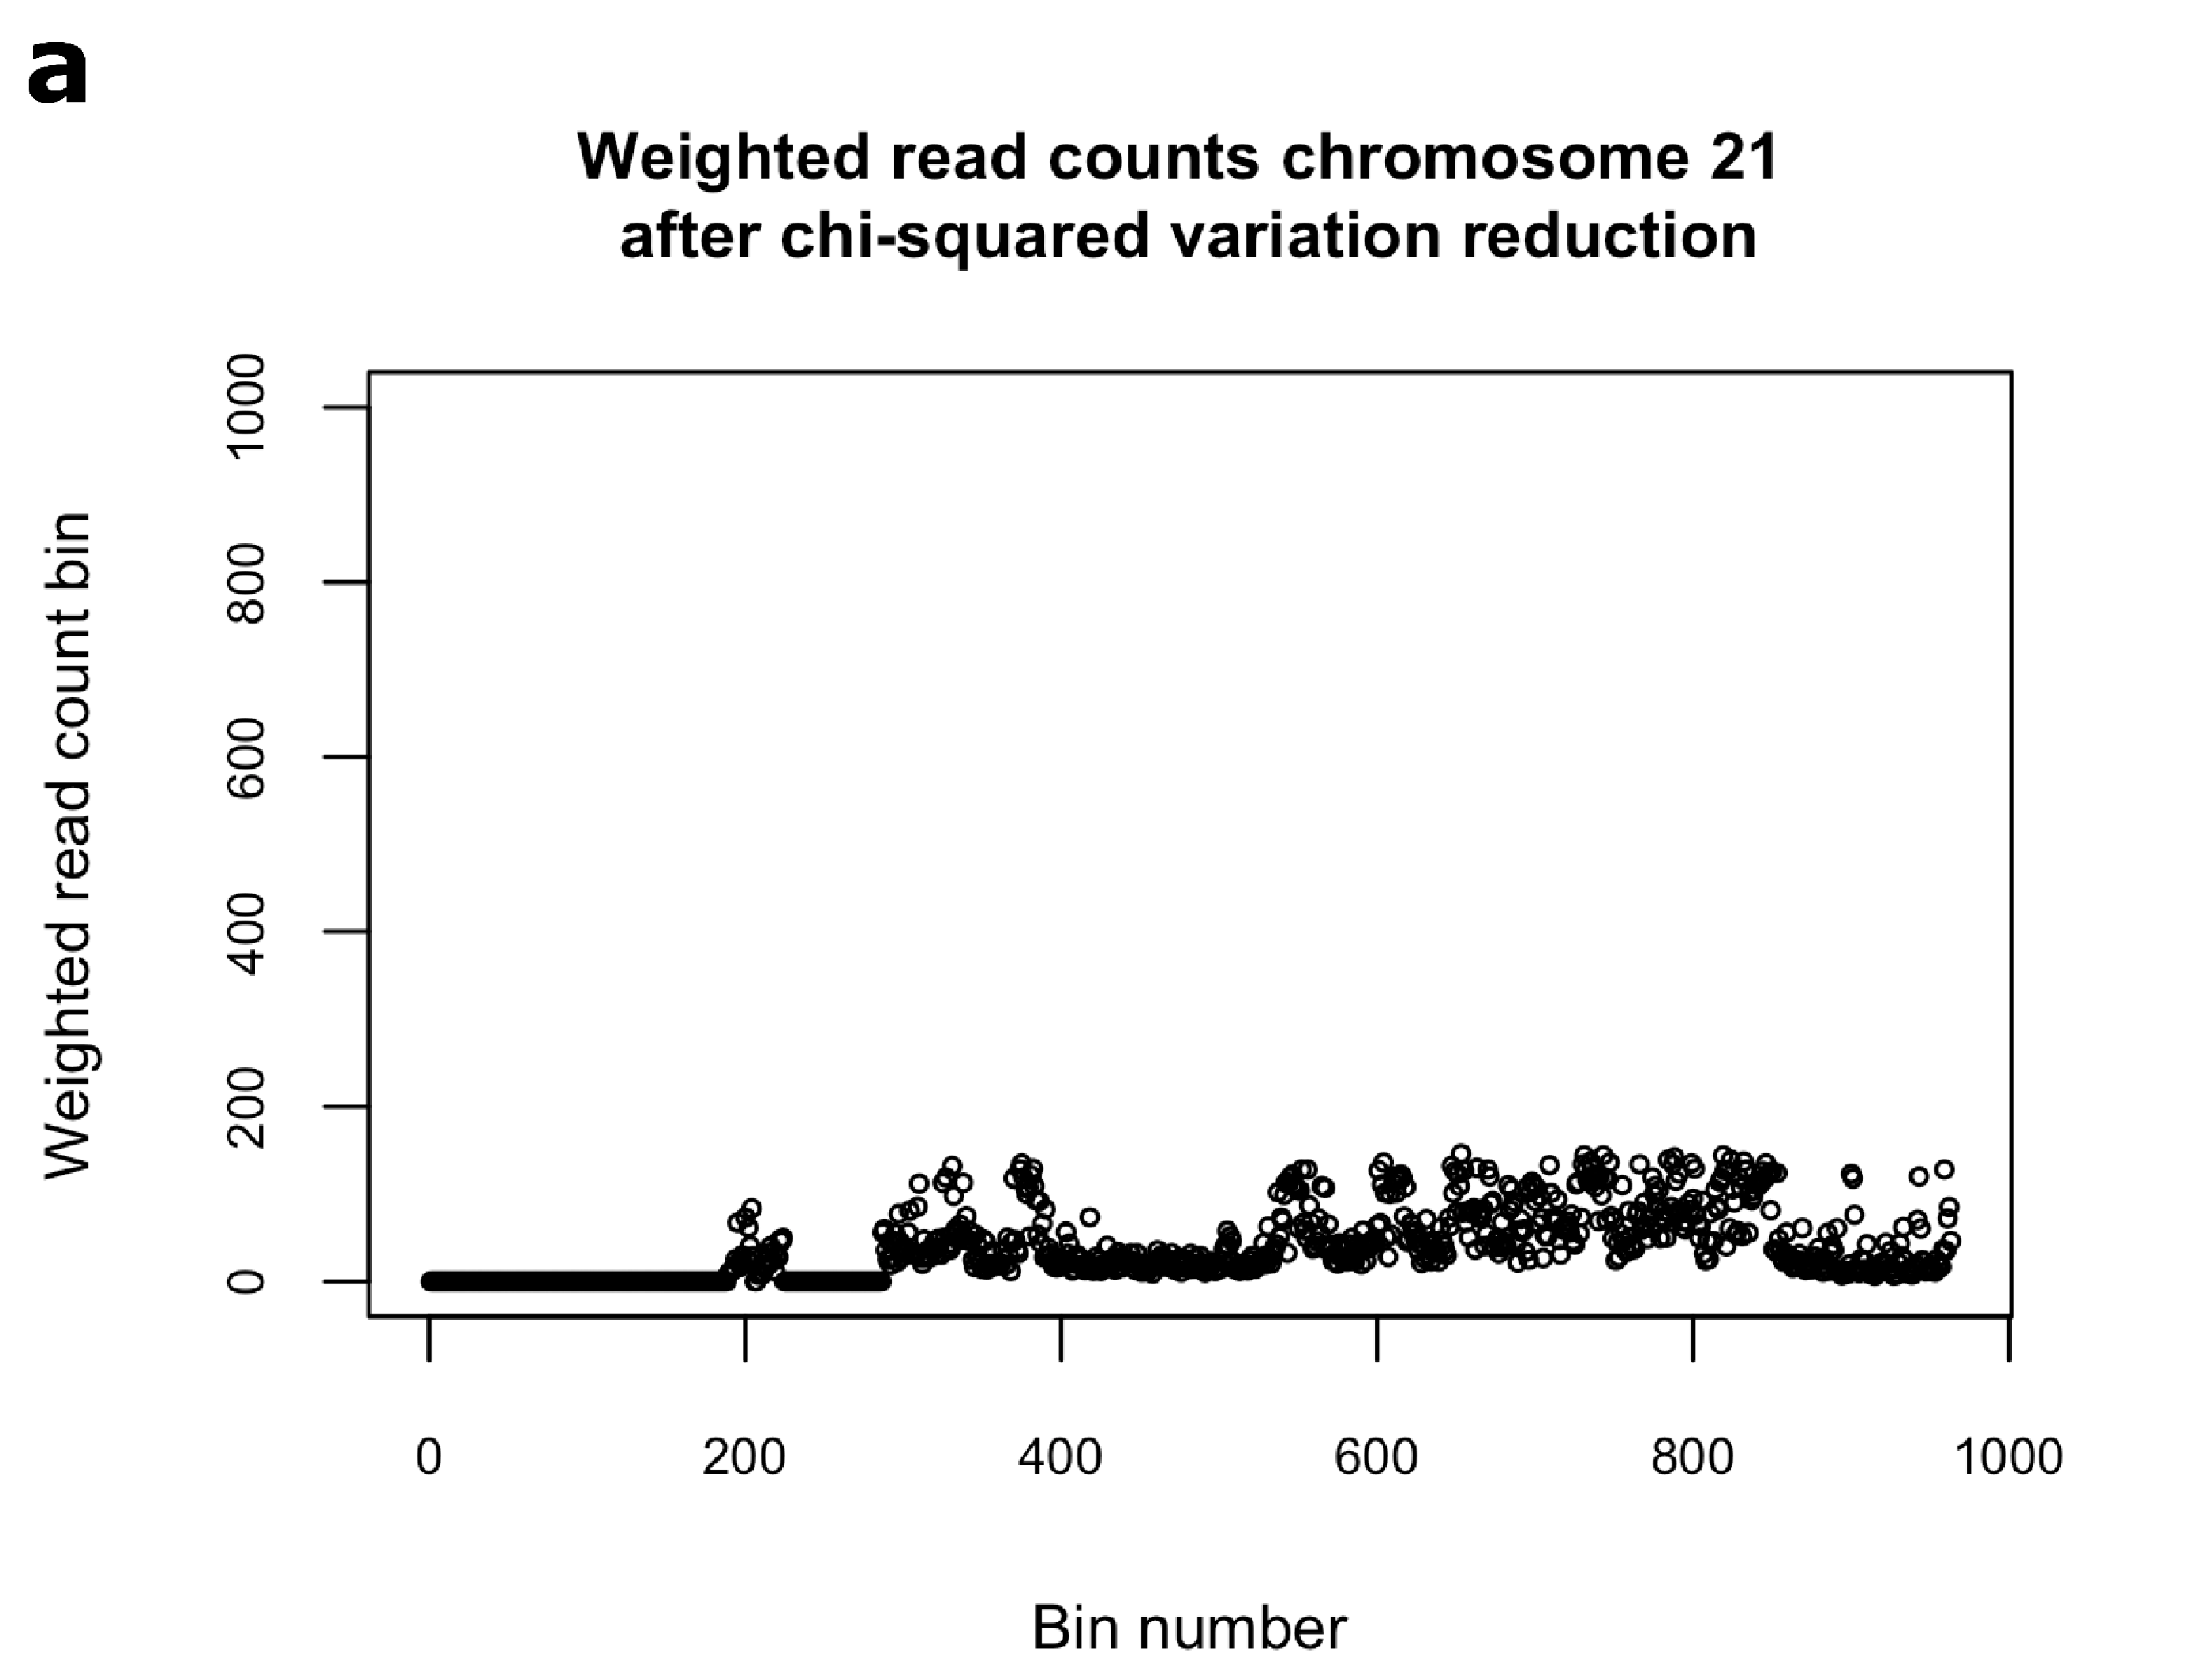
\includegraphics[width=1\linewidth]{img/NIPT_Supp1_Fig1_5a}
		\label{fig:NIPT_Supp1_Fig1_5a}
	\end{subfigure}%
	\begin{subfigure}{.5\textwidth}
		\centering
		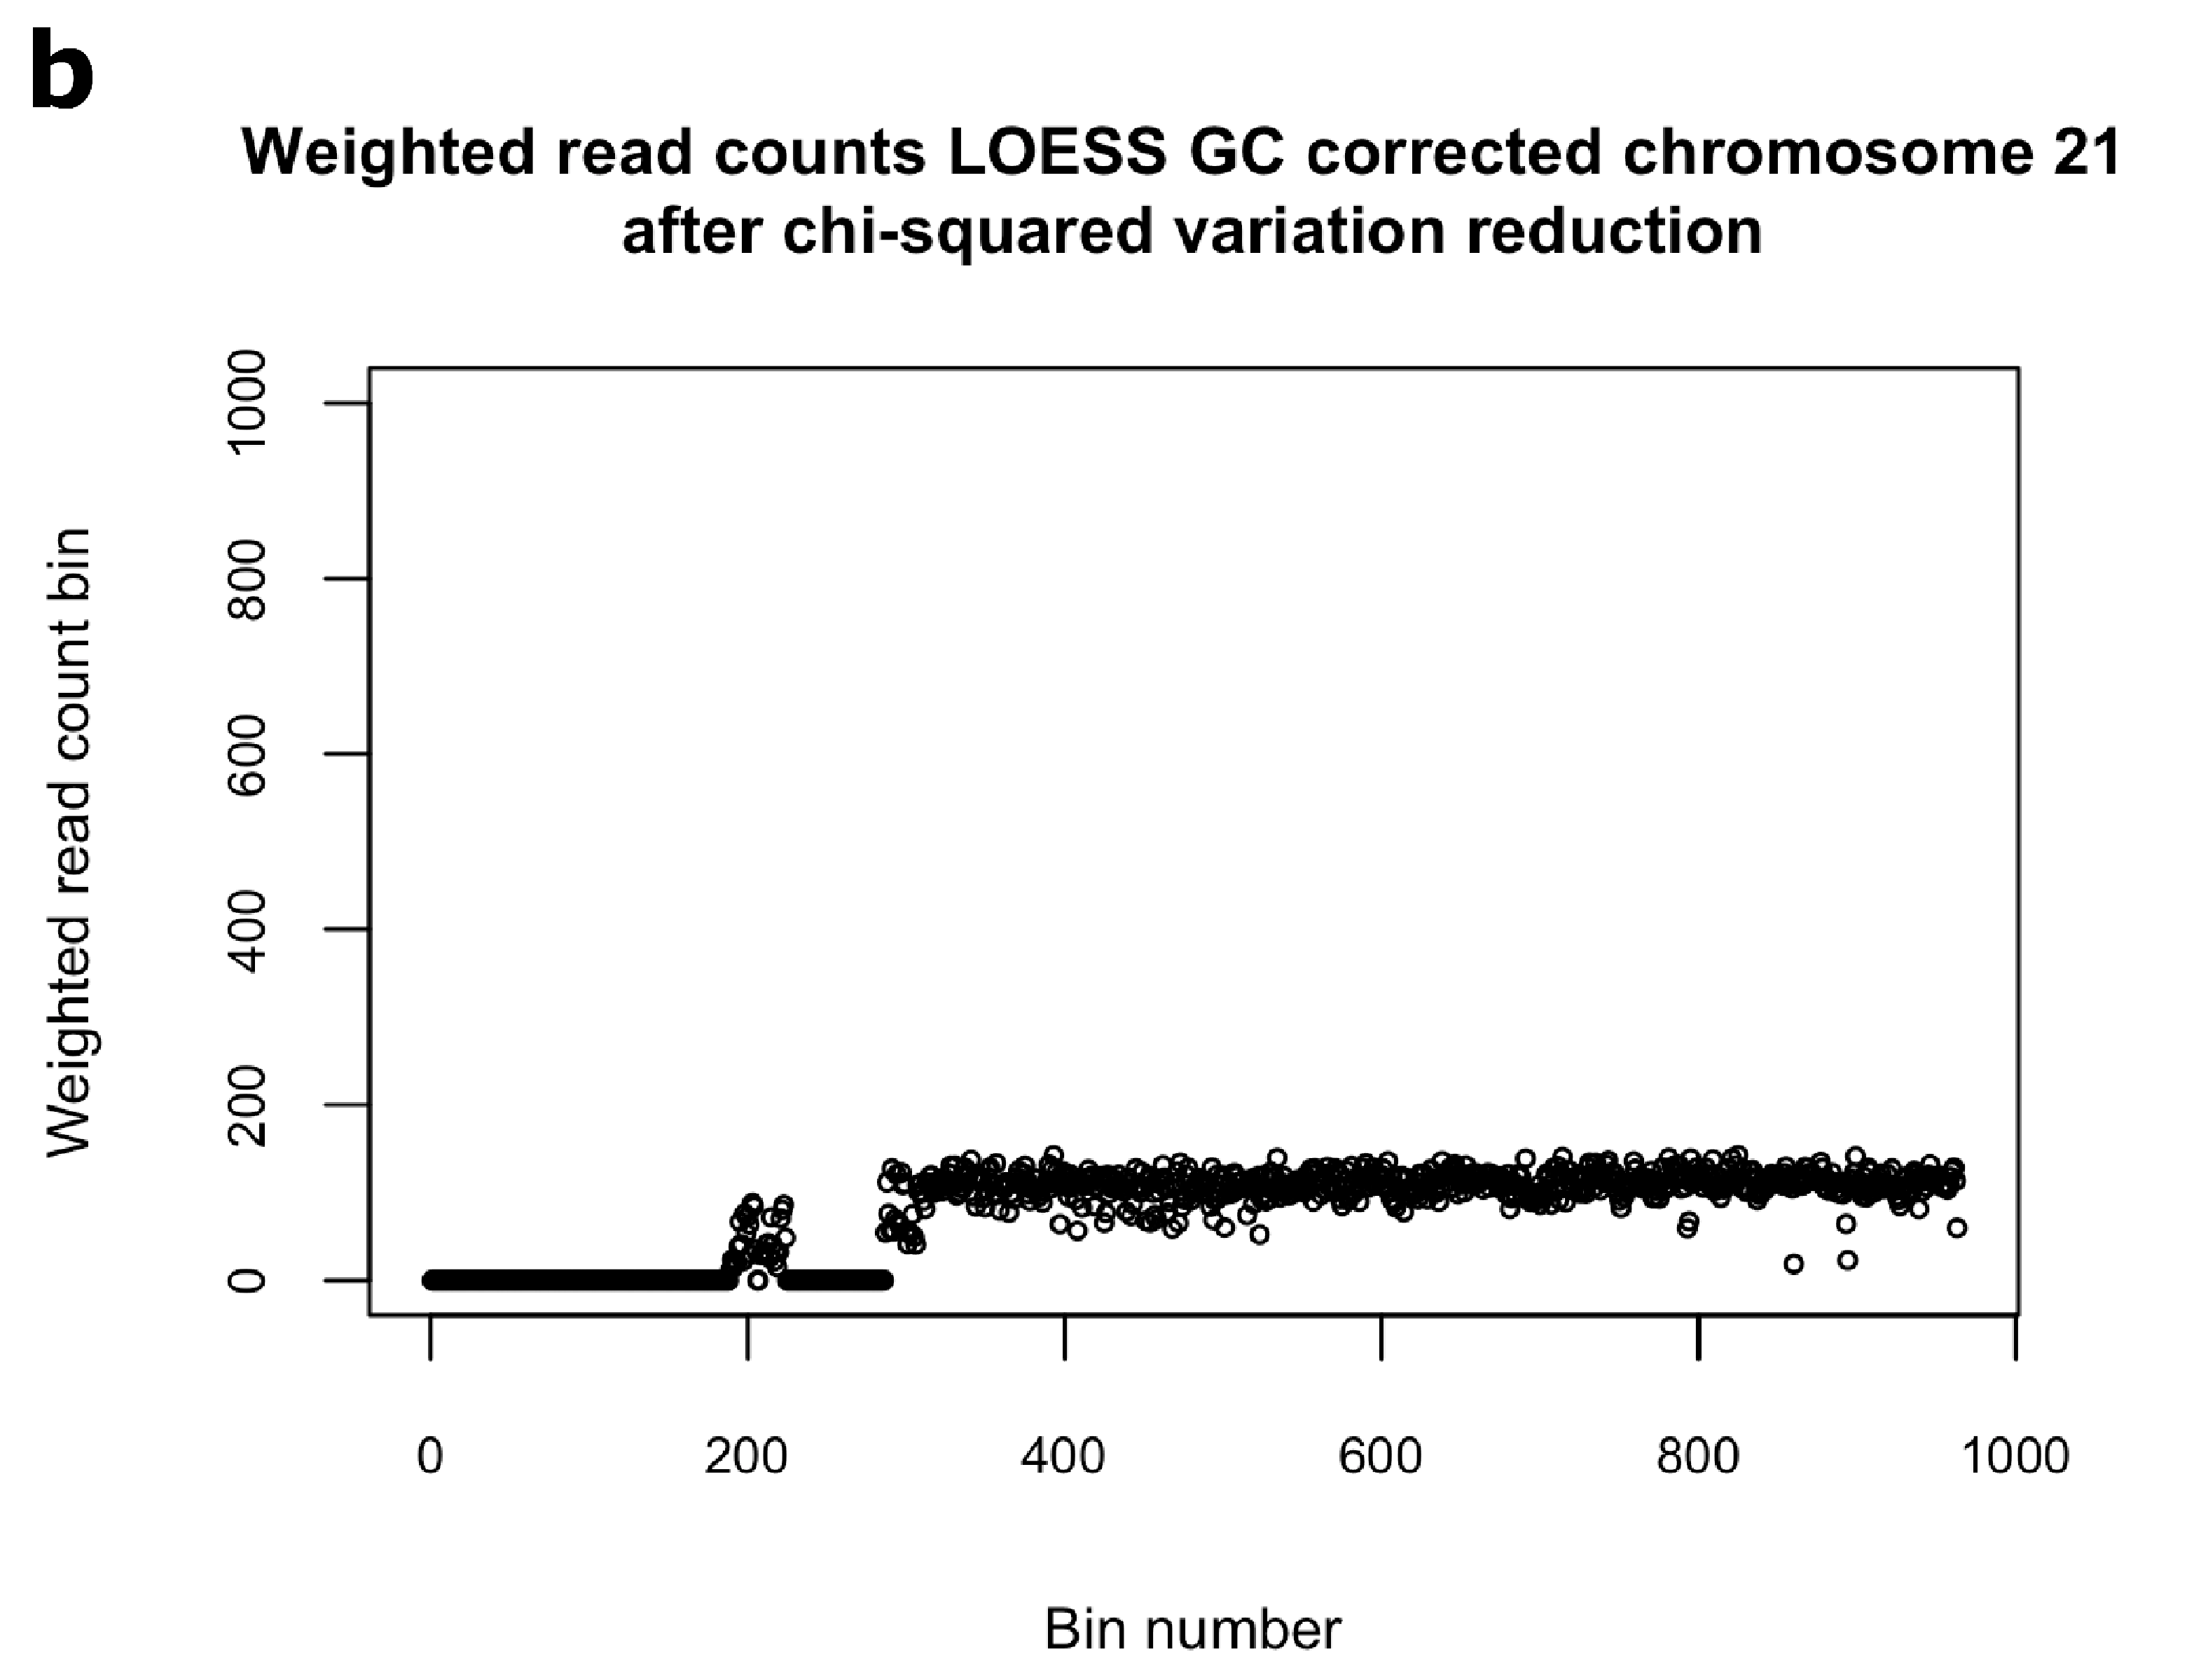
\includegraphics[width=1\linewidth]{img/NIPT_Supp1_Fig1_5b}
		\label{fig:NIPT_Supp1_Fig1_5b}
	\end{subfigure} 
	\caption[Example Weighted read counts after $\chi$\textsuperscript{2}VR]{\textbf{Weighted read counts bins chromosome 21 for one of the Illumina control group samples} \textbf{(a)} uncorrected data. \textbf{(b)} LOESS GC corrected data.}
	\label{fig:NIPT_Supp1_Fig1_5}
\end{figure}

\noindent A threshold was set at a Z-score of 3.5. In the case all the variation was introduced by chance 99.9998\% of the bins show a Z-score below 3.5. 
The variation in bins having a Z-score greater than 3.5 (overdispersed bins) is thus very unlikely to result from random variation and these bins
have a higher variability than expected. The $\chi$\textsuperscript{2}VR is based upon the assumption that there is still information present in the overdispersed bins. 
Instead of ignoring those bins, those exceeding the threshold will be weighted by dividing them by a correction factor (Fig. \ref{fig:NIPT_Supp1_Fig1_4}, Fig. \ref{fig:NIPT_Supp1_Fig1_5}).
The correction factor consists of the sum chi-squared value divided by the degrees of freedom.

Note that weighting read counts of overdispersed bins does not change the CV of those bins.
Variability between samples is not affected at bin level. However, variability between chromosomal fractions is decreased after $\chi$\textsuperscript{2}VR (Fig. \ref{fig:NIPT_Supp1_Fig1_6}).
The chromosomal fractions are defined as the number of (weighted) read counts on chromosome 21 divided by the (weighted) read count of all autosomes. 
In figure \ref{fig:NIPT_Supp1_Fig1_6} the fractions of chromosome 21 are normalized by dividing the fraction of each sample by the mean fraction of its control group.

\begin{figure}[h]
	\begin{subfigure}{.5\textwidth}
		\centering
		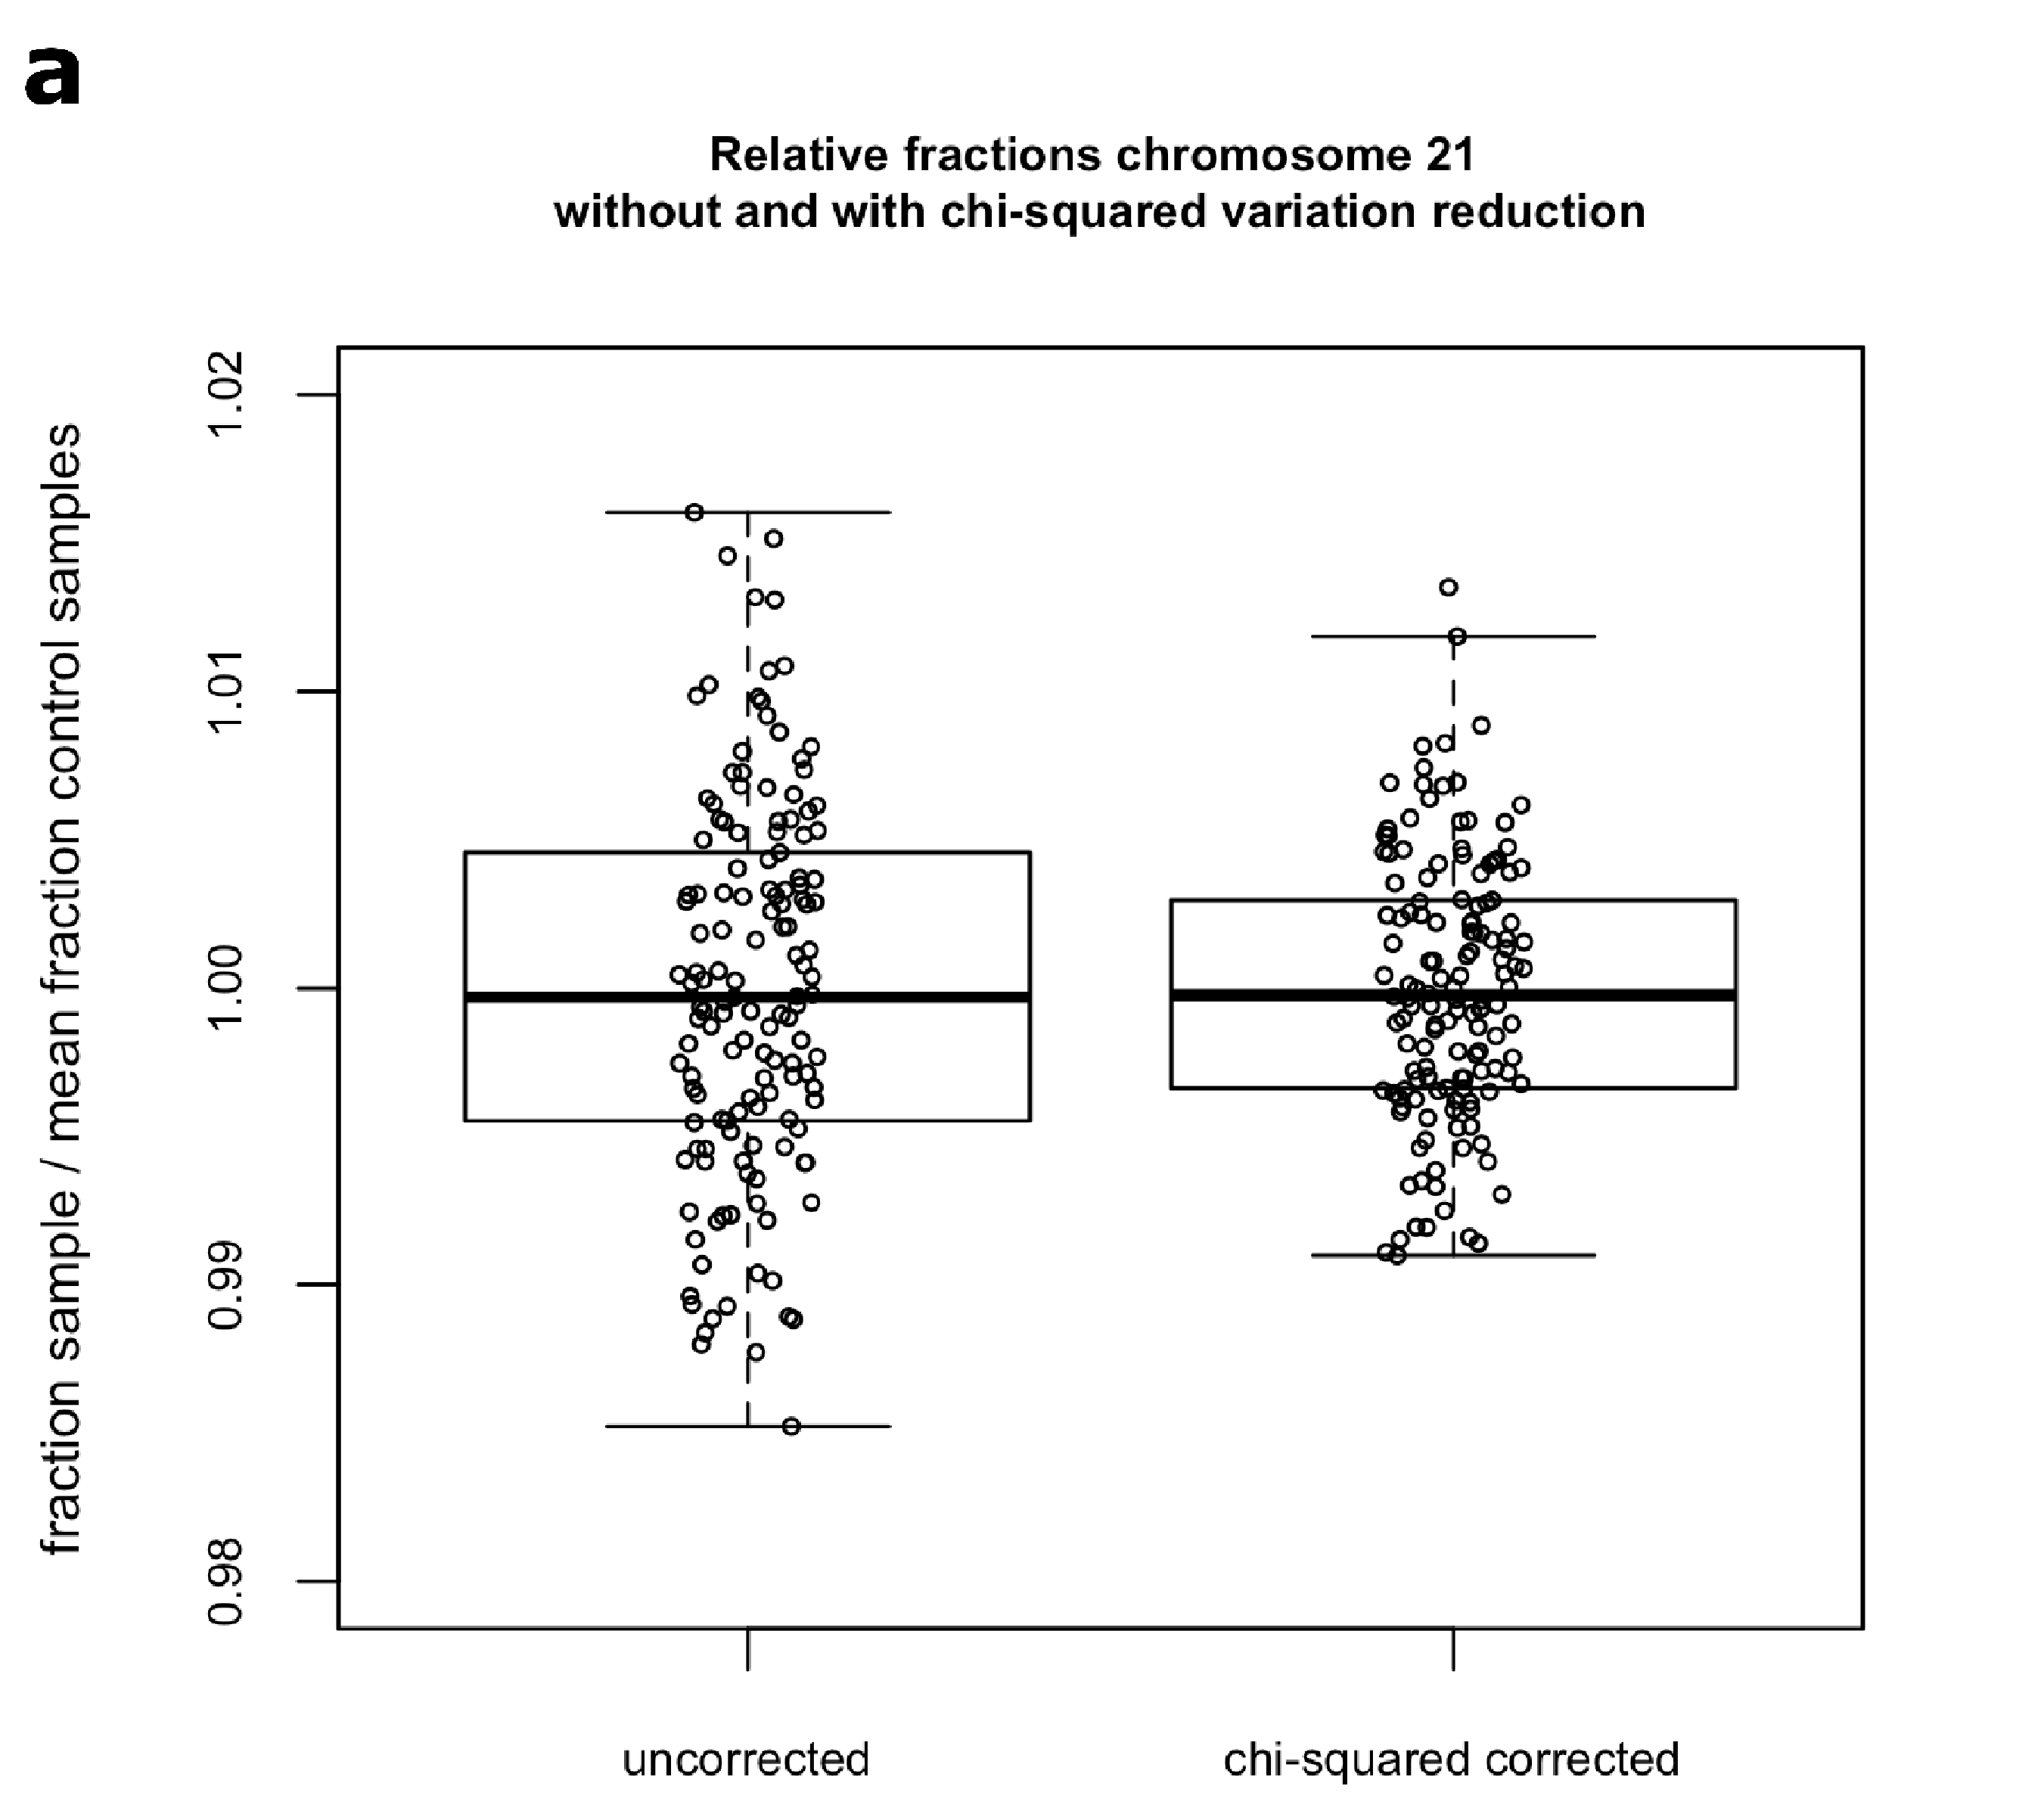
\includegraphics[width=1\linewidth]{img/NIPT_Supp1_Fig1_6a}
		\label{fig:NIPT_Supp1_Fig1_6a}
	\end{subfigure}%
	\begin{subfigure}{.5\textwidth}
		\centering
		\includegraphics[width=1\linewidth]{img/NIPT_Supp1_Fig1_6b}
		\label{fig:NIPT_Supp1_Fig1_6b}
	\end{subfigure} 
	\caption[Relative fractions chromosome 21 before and after $\chi$\textsuperscript{2}VR]{\textbf{Relative fractions chromosome 21 before and after $\chi$\textsuperscript{2}VR of Illumina control group samples} \textbf{(a)} uncorrected data. \textbf{(b)} LOESS GC corrected data.}
	\label{fig:NIPT_Supp1_Fig1_6}
\end{figure}

\sectionmark{Regression model for chromosome 13}
\section{Supplement 3: \\ Regression model for chromosome 13}\label{Supplement 3}
\sectionmark{Regression model for chromosome 13}

This supplement contains a series of graphs to visualize an example of a model upon which the RBZ is based. The input of the RBZ model are the chromosomal fractions of the control group samples. Chromosomal fractions of reads aligned to the forward strand and reads aligned to the reverse strand are considered as separate predictors, since there are consistent differences between those fractions (Supplement S2).  However, reads aligned to the forward or reverse strand are considered together for the chromosome of interest, because this yields the lowest CV. 
Table \ref{table:regression_13} and figure \ref{fig:NIPT_Supp3_Fig3_1} show a regression model using four predictors to predict the expected chromosomal fraction of chromosome 13 based upon the 142 Illumina control samples, without any variation correction. 

\begin{table}[H] %the [H] is to force the footnotes on the same page as the table
	\begin{minipage}{\textwidth}
		\caption[Coefficients of regression model chromosome 13 Illumina]{\label{table:regression_13} \textbf{Coefficients of regression model chromosome 13 Illumina}}
		\resizebox{\linewidth}{!}{\begin{tabulary}{\linewidth}{p{1.8cm}p{1.8cm}p{1.8cm}p{1.8cm}p{1.8cm}p{1.8cm}}
				\rule{0pt}{1ex} Coefficients & & & & & \\
				\rule{0pt}{1ex} & Estimate & Std. Error & t & value & Pr (\textless  \textbar t\textbar) \\
				\hline
				\rule{0pt}{1ex} Intercept & 0.018236 & 0.004737 & 3.85 & 0.00018 & \footnotemark[1] \\
				\rule{0pt}{1ex} 4F & 0.527854 & 0.056882 & 9.28 & 3.36E-16 & \footnotemark[1] \\
				\rule{0pt}{1ex} 6F & 0.391124 & 0.086029 & 4.546 & 1.19E-05 & \footnotemark[1] \\
				\rule{0pt}{1ex} 16F & -0.20697 & 0.04596 & -4.503 & 1.42E-05 & \footnotemark[1] \\
				\rule{0pt}{1ex} 1F & -0.25465 & 0.067397 & -3.778 & 0.000235 & \footnotemark[1] \\
		\end{tabulary}}
		\footnotetext{ [1] significance \textless 0.001}
		\end{minipage}
\end{table}


\begin{figure}[h]
	\includegraphics[width=0.8\linewidth]{img/NIPT_Supp3_Fig3_1}
	\caption[Example of regression model chromosome 13]{\textbf{Regression model for prediction of expected read count for chromosome 13 based upon uncorrected Illumina control group samples}}
	\label{fig:NIPT_Supp3_Fig3_1}
\end{figure}

\noindent The four predictors in the regression model are selected using stepwise regression with forward selection. 
Which predictors are selected depends on the control group. For the 142 Illumina control samples, the best predictors were reads aligned to the forward strands of chromosomes 1, 4, 6 and 16. 
The reads aligned to chromosomes 4 and 6 showed a positive correlation with the number of reads on chromosome 13, while the reads aligned to chromosomes 1 and 16 showed a negative correlation (Fig.  \ref{fig:NIPT_Supp3_Fig3_2}).
The read counts in the graphs are normalized by dividing them by the mean read count of the sample and multiplying them by the average mean read count of all control samples.

\begin{figure}[h]
	\begin{subfigure}{.5\textwidth}
		\centering
		\includegraphics[width=1\linewidth]{img/NIPT_Supp3_Fig3_2a}
		\label{fig:NIPT_Supp3_Fig3_2a}
	\end{subfigure}%
	\begin{subfigure}{.5\textwidth}
		\centering
		\includegraphics[width=1\linewidth]{img/NIPT_Supp3_Fig3_2b}
		\label{fig:NIPT_Supp3_Fig3_2b}
	\end{subfigure}
	\begin{subfigure}{.5\textwidth}
		\centering
		\includegraphics[width=1\linewidth]{img/NIPT_Supp3_Fig3_2c}
		\label{fig:NIPT_Supp3_Fig3_2c}
	\end{subfigure} 
	\begin{subfigure}{.5\textwidth}
		\centering
		\includegraphics[width=1\linewidth]{img/NIPT_Supp3_Fig3_2d}
		\label{fig:NIPT_Supp3_Fig3_2d}
	\end{subfigure}  
	\caption[Correlation between normalized read counts of chromosomes]{\textbf{Correlation betweeen normalized read counts of predictor chromosomes and normalized read counts on chromosome 13 for 142 Illumina control samples} \textbf{(a)} Chromosome 1 \textbf{(b)} chromosome 4 \textbf{(c)} chromosome 6 and \textbf{(d)} chromosome 16.}
	\label{fig:NIPT_Supp3_Fig3_2}
\end{figure}


\noindent The predicted chromosomal fraction is equal to the expected chromosomal fraction in a nontrisomy situation ($ef$). For each sample a ratio between predicted and observed chromosomal fraction is calculated, resulting in a ratio observed/predicted fraction ($of/ef$) (Fig. \ref{fig:NIPT_Supp3_Fig3_3}a).
Using these values a Z-score can be calculated for each sample (Fig. \ref{fig:NIPT_Supp3_Fig3_3}b). The general structure of the formula is equal to the standard Z-score formula:

\begin{equation*}
\frac{x - \mu}{\sigma}
\end{equation*}

\noindent Because the mean of the control group after regression is one, the coefficient of variation of the control group has the same value as the SD. Using the same structure, the RBZ can be formulated as:

\begin{equation*}
\frac{of_s / ef_s - 1}{\sqrt{\sum^n_{j=1}(of_j / ef_j - \overline{of/ef})^2 / n - 1}}
\end{equation*}

\noindent Where $s$ is the sample of interest, $j$ is an individual control sample and $n$ is the total number of control samples. 
The regression model for trisomy prediction for chromosome 13 in uncorrected Illumina data, described in table \ref{table:regression_13}, resulted in a mean fraction of 1.0000 and a CV of 0.0024 (0.24\%).

\begin{figure}[h]
	\begin{subfigure}{.5\textwidth}
		\centering
		\includegraphics[width=1\linewidth]{img/NIPT_Supp3_Fig3_3a}
		\label{fig:NIPT_Supp3_Fig3_3a}
	\end{subfigure}%
	\begin{subfigure}{.5\textwidth}
		\centering
		\includegraphics[width=1\linewidth]{img/NIPT_Supp3_Fig3_3b}
		\label{fig:NIPT_Supp3_Fig3_3b}
	\end{subfigure} 
	\caption[Ratios observed / predicted and Z-scores for chromosome 13]{\textbf{Ratios observed / predicted and Z-scores for chromosome 13 for 142 uncorrected Illumina control samples} \textbf{(a)} ratios observed / predicted \textbf{(b)} Z-scores.}
	\label{fig:NIPT_Supp3_Fig3_3}
\end{figure}

The number of predictors used in the RBZ can be as low as one or as high as all autosomes. 
However, we advise using a minimum of four predictor chromosomes, since an aberration in one of the other chromosomes (in mother or child) could influence the prediction. 
The effect of such an aberration is larger when fewer predictors are used. 
For the same reason we advise not using both the reads aligned to the forward strand and reads aligned to the reverse strand of the same chromosome in the same model.

Different independent RBZ models can be created for each analysis. 
We advise creating four different models, because reads originating from the same chromosome can be included in a maximum of two different models. Results affected by an aberration in one of the predictor chromosomes can be identified using the additional models.
\chapter[\textsl{NIPTeR}: an R package for NIPT analysis]{\textsl{NIPTeR}: an R package for fast and accurate trisomy prediction in non-invasive prenatal testing}
\chaptermark{NIPTeR: an R package for NIPT analysis}
\label{chap:NIPTeR}

{ \Large \leftwatermark{
		\put(-67,-66.5){ 1 }
		\put(-67,-91.5){ 2 }
		\put(-67,-116.5){ 3 }
		\put(-67,-141.5){ 4 }
		\put(-67,-166.5){ 5 }
		\put(-67,-191.5){ 6 }
		\put(-76.5,-225){\includegraphics[scale=0.8]{img/thumbindex.eps}} \put(-67,-216.5){ {\color{white} 7 }}
		\put(-67,-241.5){ 8 }
		\put(-67,-266.5){ 9 }
		\put(-67,-291.5){ 10 }
		\put(-67,-316.5){ 11 }
	} \rightwatermark{
		\put(350.5,-66.5){ 1 }
		\put(350.5,-91.5){ 2 }
		\put(350.5,-116.5){ 3 }
		\put(350.5,-141.5){ 4 }
		\put(350.5,-166.5){ 5 }
		\put(350.5,-191.5){ 6 }
		\put(346.5,-225){\includegraphics[scale=0.8]{img/thumbindex.eps}} \put(350.5,-216.5){ {\color{white} 7 }}
		\put(350.5,-241.5){ 8 }
		\put(350.5,-266.5){ 9 }
		\put(350.5,-291.5){ 10 }
		\put(350.5,-316.5){ 11 }
}}

\hfill \underline{BMC Bioinformatics} 2018;19:531.

\hfill DOI: \href{https://doi.org/10.1186/s12859-018-2557-8}{10.1186/s12859-018-2557-8}

\hfill PubMed ID: \href{https://www.ncbi.nlm.nih.gov/pubmed/30558531}{30558531}

\newpage

\noindent
L.F. Johansson\textsuperscript{1,2}, H.A. de Weerd\textsuperscript{1,2,3}, E.N. de Boer\textsuperscript{1}, F. van Dijk\textsuperscript{1,2}, G.J. te Meerman\textsuperscript{1}, R.H. Sijmons\textsuperscript{1}, B. Sikkema-Raddatz\textsuperscript{1}, M.A. Swertz\textsuperscript{1,2}\\

\noindent
1. University of Groningen, University Medical Center Groningen, Department of Genetics, Groningen, The Netherlands\\
2. University of Groningen, University Medical Center Groningen, Genomics Coordination Center, Groningen, The Netherlands\\
3. School of Bioscience, Systems biology research center, University of Skövde, Skövde, Sweden\\

\noindent
Received 2018 Oct 2; Accepted 2018 Dec 4; Published online 2018 Dec 17.
\\~\\


\section*{Abstract}\label{abstract}
\textbf{Background}
Various algorithms have been developed to predict fetal trisomies using cell-free DNA in non-invasive prenatal testing (NIPT). 
As basis for prediction, a control group of non-trisomy samples is needed. Prediction accuracy is dependent on the characteristics of this group and can be improved by reducing variability between samples and by ensuring the control group is representative for the sample analyzed.

\noindent\textbf{Results}
\textsl{NIPTeR} is an open-source R Package that enables fast NIPT analysis and simple but flexible workflow creation, including variation reduction, trisomy prediction algorithms and quality control. This broad range of functions allows users to account for variability in NIPT data, calculate control group statistics and predict the presence of trisomies.

\noindent\textbf{Conclusion}
\textsl{NIPTeR} supports laboratories processing next-generation sequencing data for NIPT in assessing data quality and determining whether a fetal trisomy is present. \textsl{NIPTeR} is available under the GNU LGPL v3 license and can be freely downloaded from \sloppy{https://github.com/molgenis/NIPTeR} or CRAN.


\section{Background}\label{Background}
Non-invasive prenatal testing (NIPT) is rapidly becoming the new standard in prenatal screening for fetal aneuploidy \cite{Allyse_2015}. 
In NIPT, cell-free DNA from the pregnant woman’s blood plasma, which consists of both maternal and fetal DNA fragments, is analysed. 
Next to SNP-based methods \cite{Hall_2014}, low-coverage whole genome next-generation sequencing (NGS) is often used \cite{Chiu_2008,Sehnert_2011}, and various algorithms, software programs and packages have been developed to analyse this type of data \cite{Chen_2011b, Straver_2013, Yang_2017, Sauk_2018, Phan_2018}. 
In literature, many methods have been described that depend on a statistical comparison between a sample of interest and a reference set of non-trisomy control samples \cite{Chiu_2008,Sehnert_2011,Fan_2010,Johansson_2017}. 
The \textsl{RAPIDR} and \textsl{DASAF} R packages, for instance, have been described \cite{Lo_2014,Liu_2016} and they made several of these algorithms available, including GC-correction, the standard Z-score and the Normalized Chromosome Value (NCV), to create an analysis workflow in R. 
However, those packages lack features like chi-squared-based variation reduction ($\chi$\textsuperscript{2}VR), regression-based Z-score (RBZ) and Match QC. 
These are all algorithms that we have extensively discussed before \cite{Johansson_2017}. 
In short, $\chi$\textsuperscript{2}VR detects chromosomal regions that have a higher variability than expected by chance and reduces their weight so that, after correction, they have less impact on the fraction of reads mapped to the different chromosomes. 
The RBZ is an alternative Z-score calculation based on stepwise regression with forward selection. 
In the RBZ positive or negative correlation between chromosomal fractions is used to predict the number of reads to map onto the chromosome of interest if no trisomy is present. 
The Match QC score is a sum-of-squares-based approach to compare chromosomal fractions between the test sample and controls, and it provides a measure by which to determine whether a control group is representative for a specific sample. 
Here we report \textsl{NIPTeR}, an R package that provides fast NIPT analysis for research and diagnostics and provides users with multiple methods for variation reduction, prediction and quality control based upon comparison of a sample with a set of negative control samples.

\section{Implementation}\label{Implementation}
\textsl{NIPTeR} users can create different workflows for variation reduction and aneuploidy prediction using thirteen functions as building blocks (Fig. \ref{fig:NIPTeR_Fig1}).
A stepwise practical example for using these building blocks is presented as a case report in Additional file 1.

\begin{figure}
	\includegraphics[width=1.0\linewidth]{img/NIPTeR_Fig1}
	\caption[Workflow and functions of \textsl{NIPTeR}]{Workflow and functions of \textsl{NIPTeR}. \textbf{a} A BAM file is transformed into an NIPTSample object; \textbf{b} a series of NIPTSample objects can then be transformed into an NIPTControlGroup object; \textbf{c} optional LOESS or weighted bin GC correction; \textbf{d} optional chi-squared-based variation reduction; \textbf{e} optional comparison of NIPTSample and NIPTControlGroup and possible selection of a subset that best-matches the control group samples; \textbf{f} three different prediction methods: Z-score, normalized chromosome value or regression-based Z-score; \textbf{g} optional check of control group statistics}
	\label{fig:NIPTeR_Fig1}
\end{figure}

\textsl{NIPTeR} analysis uses two core objects. 
The first object is \textsl{NIPTSample}, which contains the counts of aligned sequence reads in 50,000 bp bins for a specific sample. 
The second object is \textsl{NIPTControlGroup}, which contains a series of NIPTSamples for comparison. Users generate \textsl{NIPTSample} using the function \textsl{bin\_bam\_sample}, which needs a BAM file \cite{Li_2009} as input. 
The user can optionally select to count reads mapped to the forward and reverse strands separately, so that they can each be used as a separate predictor. 
The \textsl{as\_control\_group} function converts a series of \textsl{NIPTSample} objects into a \textsl{NIPTControlGroup}. 
Within \textsl{NIPTeR}, users can manage an existing \textsl{NIPTControlGroup} using the \textsl{add\_samples\_controlgroup}, \textsl{remove\_sample\_controlgroup} and \textsl{remove\_duplicates\_controlgroup} functions.

Both \textsl{NIPTSample} and \textsl{NIPTControlGroup} can undergo one or more variation reduction steps to adjust the bin read counts, either using the \textsl{gc\_correct} function for weighted bin GC correction \cite{Fan_2010} or LOESS GC correction \cite{Chen_2011} or the \textsl{chi\_correct} function for $\chi$\textsuperscript{2}VR. 
Each \textsl{NIPTSample} object shows the correction status for the autosomes and the sex chromosomes separately and indicates which variation reduction methods have been performed (or that they are ‘uncorrected’). 
$\chi$\textsuperscript{2}VR can be applied to uncorrected or GC-corrected samples, and makes use of a NIPTSample and a NIPTControlGroup having an identical correction status.

Using the fractions of reads mapped to the different chromosomes, trisomy prediction can be generated for a given \textsl{NIPTSample} based on the \textsl{NIPTControlGroup} using three different prediction algorithms: (1) \textsl{calculate\_z\_score}, which uses a standard Z-score \cite{Chiu_2008}; (2) \textsl{calculate\_ncv\_score}, which uses an NCV \cite{Sehnert_2011}; and (3) \textsl{perform\_regression}, which uses RBZ. 
All three trisomy prediction functions use \textsl{NIPTControlGroup} to calculate the expected fraction of reads on the chromosome of interest. 
For NCV, this calculation is done in a separate function, \textsl{prepare\_ncv}, because the calculation is time-intensive and only has to be performed once for each \textsl{NIPTControlGroup}. 
The prediction functions then compare the observed fraction of reads of the chromosome of interest in the \textsl{NIPTSample} with the expected fraction. 
In NCV and RBZ calculations, users have the option of excluding selected chromosomes as predictors. Since chromosomes 13, 18 and 21 are the most likely candidates for a trisomy, these are excluded by default, but users do have the option of including them. 
The functions \textsl{prepare\_ncv} and \textsl{perform\_regression} provide users the option of using a train and test set to prevent over-fitting the models they create.

In addition to providing Z-scores, the functions also produce control group statistics. 
The function \textsl{match\_control\_group} provides a Match QC score, a calculation that shows how well the sample fits within the control group based on the fraction of reads mapped to the different chromosomes, a measure that can be shown in a report. 
Alternately, users can select a subset of best-matching control samples as a sample-specific control group using the arguments mode = "report" or "subset". 
When a sample has an anomalously high Match QC score, the control samples being used are not suitable as a control group for the sample being analyzed. 
A second quality control function, \textsl{diagnose\_control\_group}, calculates Z-scores for all samples and chromosomes in a \textsl{NIPTControlGroup} as well as the mean, standard deviation and Shapiro-Wilk test of those Z-scores. 
This information can be used to curate the control group as explained in detail in Additional file 1.

\section{Results}\label{Results}
\subsection{Workflow}
All these \textsl{NIPTeR} building blocks can be combined into an analysis workflow. For example, the \textsl{NIPTeR} workflow for the Fan \& Quake analysis \cite{Fan_2010}, using a weighted bin GC correction and a standard Z-score prediction for trisomy 21, and given a GC-corrected control group is: \\* \vspace{-\baselineskip} %Make distance between lines smaller


\begin{alltt}
	\footnotesize  
		\noindent\textgreater\ NIPTsample \textless- bin\_bam\_sample(bam\_filepath = \\\indent "/Path/to/bam/sample.bam") \\
		\textgreater\ NIPTsample\_gc \textless- gc\_correct(nipt\_object =  NIPTsample,\\\indent method = "bin") \\
		\textgreater\ Zscore21\_NIPTsample \textless- \\\indent  calculate\_z\_score(nipt\_sample = NIPTsample\_gc,\\\indent nipt\_control\_group = NIPTControlGroup\_gc, \\\indent chromo\_focus = 21) \\*
\end{alltt}

\noindent In addition, control group statistics and the match control of the sample to the control group can be performed: \\* \vspace{-\baselineskip}

\begin{alltt}
	\footnotesize  
		\noindent\textgreater\ NIPTcontrol\_diagnose \textless- diagnose\_control\_group(nipt\_control\_group \\\indent= NIPT\_control\_group\_gc) \\
		\textgreater\ MatchQC \textless- match\_control\_group(nipt\_sample = NIPTsample\_gc, \\\indent nipt\_control\_group = NIPT\_control\_group\_gc, mode = "report")
\end{alltt}

\subsection{Prediction and control group statistics}
The output formats of the \textsl{calculate\_z\_score} and \textsl{calculate\_ncv\_score} functions are similar. An example result of the main output reads: \\* \vspace{-\baselineskip}

\begin{alltt}
	\footnotesize 
\noindent Zscore21\_NIPTsample\$sample\_Zscore \\ 
\baselineskip=12pt [1] 0.4575612 \\ 
 Zscore21\_NIPTsample\$control\_group\_statistics \\ 
\baselineskip=4pt mean \hspace{20mm} SD \hspace{22mm} Shapiro\_P\_value  \\ 
 1.380646e-02 \hspace{7mm} 7.184378e-05 \hspace{5mm} 9.498096e-01 \\*
\end{alltt}

\noindent Here, the Z-score is 0.45, which falls within the -3 to 3 range and leads to the conclusion that this sample does not have a trisomy 21. 
The control\_group\_statistics show the mean fraction of sequence reads mapping to chromosome 21 and the standard deviation (SD) of the fractions between the control samples. 
The Shapiro\_P\_value tests for control group normality, and control groups with a value above 0.05 can be considered to be normally distributed. 

\newpage
The output of \textsl{perform\_regression} is slightly different and gives four predictions based on different models when set to the default setting: \\* \vspace{-\baselineskip}

\begin{alltt}
\tiny 
\noindent \hspace{14mm}	Prediction\_set\_1	\hspace{3mm} Prediction\_set\_2 \hspace{3mm} Prediction\_set\_3 \hspace{3mm} Prediction\_set\_4 \\
Z\_score\_sample  \hspace{0mm} 0.695389767405796 \hspace{2mm} 0.436463271170429 \hspace{1mm} 0.437555582217223 \hspace{1mm} -0.268842730284741 \\
CV \hspace{12mm}	0.00536568258297721 \hspace{0.2mm} 0.00502335300817695 0.00483989627449594 0.00486660271957713 \\
cv\_types  \hspace{6mm}	Practical\_CV \hspace{6mm} Practical\_CV \hspace{6.5mm} Practical\_CV \hspace{6.6mm} Practical\_CV \\
P\_value\_shapiro \hspace{0mm}	0.430190936876808 \hspace{2mm} 0.844844184734285 \hspace{1mm} 0.478810106756347 \hspace{1.2mm} 0.606229054979589 \\
Pred\_chrom\footnote{In practice Pred\_chrom is written in full as: Predictor\_chromosomes. For layout purposes a shorthand is used here.} \hspace{4mm} 3F  1F  2R  7F \hspace{4.5mm}	3R  22F  1R  5R \hspace{3.7mm} 6R  10F  8R  17F \hspace{2.5mm} 20F  12F  19R  14F \\
Mean\_test\_set \hspace{2mm} 0.998406705791639 \hspace{1.7mm}	0.997692920712523 \hspace{1.3mm} 0.998044728541847 \hspace{1.6mm} 0.997802000172399 \\
CV\_train\_set \hspace{3mm} 0.00441576466562767 \hspace{0mm} 0.004609720864648 \hspace{0.9mm} 0.00479265227193279 \hspace{0.6mm}0.00492160650642337 \\*
\end{alltt}

\noindent Here, in addition to the RBZ, the coefficient of variation (CV) of the test set is given as a measure of control group variability. 
The type of CV is given as well, in which “Practical CV” is the true CV. If there is a risk of over-fitting the model on the control set, a theoretical CV is used. 
In addition to the Shapiro P value, \textsl{perform\_regression} reports the mean of the test set (which should be close to one) and the CV of the training set (based on which the chromosomes used to create the prediction model are selected), where reads mapped to the forward and reverse strands are used as separate entities.

\subsection{Quality control}
Using the \textsl{diagnose\_control\_group} function, control samples that have outliers that could hamper prediction can be detected. \\*  \vspace{-\baselineskip}


\begin{alltt}
	\footnotesize 
\noindent\textgreater\ NIPTcontrol\_diagnose\$abberant\_scores \medskip\\
\indent Chromosome\hspace{0mm} Sample\_name \hspace{0mm} Z\_score \\
1 \baselineskip=4pt\hspace{1mm} 17F \hspace{11mm} sample21 \hspace{4mm} 3.13281485801102 \\
2 \baselineskip=4pt\hspace{1mm} 1R  \hspace{11mm} sample21 \hspace{4mm} 3.1290608434065 \\
3 \baselineskip=4pt\hspace{1mm} 17R \hspace{11mm} sample21 \hspace{4mm} 3.33995848430216 \\
4 \baselineskip=4pt\hspace{1mm} 22R \hspace{11mm} sample24 \hspace{4mm} 3.08496372975161 \\
… \\
19 \baselineskip=4pt\hspace{1mm}8F \hspace{13mm}  sample21 \hspace{4mm} -3.85723794269498 \\
20 \baselineskip=4pt\hspace{1mm}5R \hspace{13mm}  sample21 \hspace{4mm} -3.16594249087773 \\
21 \baselineskip=4pt\hspace{1mm}16R\hspace{13mm}  sample21 \hspace{4mm} -3.5467264109158 \\*
\end{alltt}



\noindent This example shows that, for many chromosomes in sample 21 one or both of the strands have a Z-score higher than 3. 
This means that there is more variability in this sample than expected, pointing to a low quality sample. 
As explained in more detail in Additional file 1, we recommend that users remove samples that have more than one aberrant score (Z-score outside the -3 to 3 range) from the control group.

When looking at the individual Match QC scores of the GC corrected \textsl{NIPTSample} compared to the GC corrected \textsl{NIPTControlGroup}, the list of sum of squares of differences in chromosomal fractions of the test sample compared to each control sample is shown: \\*  \vspace{-\baselineskip}


\begin{alltt}
	\footnotesize 
\noindent \hspace{15mm} Sum\_of\_squares \\
sample86 \baselineskip=4pt\hspace{1mm} 1.919715e-07 \\
sample74 \baselineskip=4pt\hspace{1mm} 2.155461e-07 \\
… \\
sample40 \baselineskip=4pt\hspace{1mm} 1.089867e-06 \\
sample21 \baselineskip=4pt\hspace{1mm} 2.028651e-06 \\
\end{alltt}

\noindent In general, the lower the sum of squares, the more representative a control sample is for the test sample. 
The average of all sum of squares for an NIPTSample is the Match QC score. 
A Match QC score for a specific sample that falls outside 3 SD of the control group Match QC, indicates that the control group is not suitable for analysis of the sample.

Further examples and results can be found in the \textsl{NIPTeR} package vignette \cite{Johansson_2016a} and the case report provided in Additional file 1. 
A demonstration of the \textsl{NIPTeR} GC-correction methods is given in Additional file 2 and a comparison of \textsl{NIPTeR} results with manual calculations is available for the $\chi$\textsuperscript{2}VR in Additional file 3 and for the prediction methods and Match QC score in Additional file 4.

The \textsl{NIPTeR} package requires R 3.1.0 or higher, the stats and sets packages as available on CRAN, and the RSamtools and S4Vectors Bioconductor packages.

\subsection{Performance}
\textsl{NIPTeR} performance was tested on three different machines and operating systems (Additional file 5). 
Given a pre-processed control group of 100 samples, one sample was processed in 3 to 4 min (on average), including both GC correction and $\chi$\textsuperscript{2}VR and using the Z-score and RBZ as prediction algorithms for chromosomes 13, 18 and 21. 
NCV analysis was performed in an additional 1 to 6 min using a maximum number of 6 to 9 chromosomes as denominator.

\section{Conclusion}\label{Conclusion}
\textsl{NIPTeR} allows for fast NIPT analysis and flexible workflow creation and includes variation correction and prediction algorithms as well as QC control. 
Algorithms used in \textsl{NIPTeR} are validated as described in Johansson and de Boer et al. \cite{Johansson_2017}\footnote{Included in this thesis as chapter 6.}. 
\textsl{NIPTeR} is available under the GNU GPL open source license and can be freely downloaded from https://github.com/molgenis/NIPTeR or CRAN.

\section{Availability and requirements}
\textbf{Project name:} NIPTeR. \\
\textbf{Project home page:} https://CRAN.R-project.org/package=NIPTeR \\
\textbf{Source page:} https://github.com/molgenis/NIPTeR \\
\textbf{Operating system(s):} Linux, MacOS, Windows. \\
\textbf{Programming language:} R. \\
\textbf{Other requirements:} R (3.1.0 or higher), RSamtools, sets, stats, S4Vectors. \\
\textbf{Licence:} GNU Lesser General Public License v3.0. \\
\textbf{Any restrictions to use by non-academics:} none

\section*{Acknowledgments}\label{Acknowledgments} 
We thank Kate Mc Intyre for editorial advice.

\section*{Authors’ contributions}
LJ is the main author. 
LJ and HdW conceived and designed the NIPTeR package. 
Together with FvD they developed and implemented the application. 
LJ, HdW, EdB and GtM designed and validated algorithms and implementation. 
RS, BS and MS were responsible for project administration and supervision. 
All authors read and approved the final version of this manuscript.

\section*{Ethics approval and consent to participate}
Not applicable.

\section*{Consent for publication}
Not applicable.

\section*{Competing interests}
The authors declare that they have no competing interests.

\section{Additional files}\label{Additional files}
Additional files can be accessed online: \\
\sloppy{https://bmcbioinformatics.biomedcentral.com/articles/10.1186/s12859-018-2557-8}




\chapter[NIPTRIC: a tool for clinical interpretation of NIPT results]{NIPTRIC: an online tool for clinical interpretation of non-invasive prenatal testing (NIPT) results}
\chaptermark{NIPTRIC: clinical interpretation of NIPT results}
\label{chap:NIPTRIC}

{ \Large \leftwatermark{
		\put(-67,-66.5){ 1 }
		\put(-67,-91.5){ 2 }
		\put(-67,-116.5){ 3 }
		\put(-67,-141.5){ 4 }
		\put(-67,-166.5){ 5 }
		\put(-67,-191.5){ 6 }
		\put(-67,-216.5){ 7 }
		\put(-76.5,-250){\includegraphics[scale=0.8]{img/thumbindex.eps}} \put(-67,-241.5){ {\color{white} 8 }}
		\put(-67,-266.5){ 9 }
		\put(-67,-291.5){ 10 }
		\put(-67,-316.5){ 11 }
	} \rightwatermark{
		\put(350.5,-66.5){ 1 }
		\put(350.5,-91.5){ 2 }
		\put(350.5,-116.5){ 3 }
		\put(350.5,-141.5){ 4 }
		\put(350.5,-166.5){ 5 }
		\put(350.5,-191.5){ 6 }
		\put(350.5,-216.5){ 7 }
		\put(346.5,-250){\includegraphics[scale=0.8]{img/thumbindex.eps}} \put(350.5,-241.5){ {\color{white} 8 }}
		\put(350.5,-266.5){ 9 }
		\put(350.5,-291.5){ 10 }
		\put(350.5,-316.5){ 11 }
}}

\hfill \underline{Scientific Reports} 2016;6:38359.

\hfill DOI: \href{https://doi.org/10.1038/srep38359}{10.1038/srep38359}

\hfill PubMed ID: \href{https://www.ncbi.nlm.nih.gov/pubmed/27917919}{27917919}

\newpage

\noindent
B. Sikkema-Raddatz\textsuperscript{1}, L.F. Johansson\textsuperscript{1,2,*}, E.N. de Boer\textsuperscript{1,*}, Elles M.J. Boon\textsuperscript{3}, R.F. Suijkerbuijk\textsuperscript{1}, K. Bouman\textsuperscript{1}, C.M. Bilardo\textsuperscript{4}, M.A. Swertz\textsuperscript{2}, M. Dijkstra\textsuperscript{2}, I.M. van Langen\textsuperscript{1}, R.J. Sinke\textsuperscript{1}, G.J. te Meerman\textsuperscript{1} \\

\noindent
1. University of Groningen, University Medical Center Groningen, Department of Genetics, Groningen, The Netherlands\\
2. University of Groningen, University Medical Center Groningen, Genomics Coordination Center, Groningen, The Netherlands\\
3. Leiden University Medical Center, Department of Clinical Genetics, Laboratory for Diagnostic Genome Analysis, Leiden The Netherlands\\
4. University of Groningen, University Medical Center Groningen, Department of Obstetrics and Gynaecology, Groningen, The Netherlands\\

\noindent
Received 2016 May 17; Accepted 2016 Nov 9; Published online 2017 Dec 5.
\\~\\



\section*{Abstract}\label{abstract}
To properly interpret the result of a pregnant woman’s non-invasive prenatal test (NIPT), her a priori risk must be taken into account in order to obtain her personalised a posteriori risk (PPR), which more accurately expresses her true likelihood of carrying a foetus with trisomy. 
Our aim was to develop a tool for laboratories and clinicians to calculate easily the PPR for genome-wide NIPT results, using diploid samples as a control group. 
The tool takes the a priori risk and Z-score into account. 
Foetal DNA percentage and coefficient of variation can be given default settings, but actual values should be used if known. 
We tested the tool on 209 samples from pregnant women undergoing NIPT. 
For Z-scores \textless 5, the PPR is considerably higher at a high a priori risk than at a low a priori risk, for NIPT results with the same Z-score, foetal DNA percentage and coefficient of variation. However, the PPR is effectively independent under all conditions for Z-scores above 6. 
A high PPR for low a priori risks can only be reached at Z-scores \textgreater 5. 
Our online tool can assist clinicians in understanding NIPT results and conveying their true clinical implication to pregnant women, because the PPR is crucial for individual counselling and decision-making.

\section{Introduction}\label{introduction}
Non-invasive prenatal testing (NIPT) for foetal aneuploidies, by analysing cell-free DNA in maternal blood, has been offered to pregnant women increasingly since 2011 [reviews refs \cite{Benn_2013,Norwitz_2013,Gil_2013}]. 
Large clinical studies including about 150,000 pregnancies have reported a sensitivity and specificity for NIPT of more than 99\% for foetal trisomy 13 or 21, and of 98\% for trisomy 18 [refs \cite{Zhang_2015} and \cite{Norton_2015}, reviews refs \cite{Benn_2013} and \cite{Norwitz_2013}]. 
This performance of NIPT in the general population of pregnant women \cite{Gil_2013,Zhang_2015,Norton_2015,Dan_2012,Nicolaides_2012,Fairbrother_2013,Lau_2014,Bianchi_2014} appears to be similar for both low-risk and high-risk pregnancies \cite{Zhang_2015,Norton_2015,Bianchi_2014,Dar_2014}1.

NIPT can identify pregnancies at risk for a trisomy and is therefore a screening tool, not a diagnostic test. 
For an individual woman, a positive NIPT result with a sensitivity and specificity of more than 99\% does not mean that she actually has more than a 99\% chance of carrying a foetus with a trisomy. 
Her true likelihood depends not only on her NIPT result, but also on the prevalence of the anomaly in the population she belongs to \cite{Morain_2013}, which is expressed as an a priori risk. 
Thus, her individual a priori risk for a specific foetal trisomy is based on her age, the gestational age at which NIPT is performed, and the results of other screening tests such as the first trimester combined test (FCT). 
The result of a NIPT for an individual woman in most of the genome-wide methods is calculated as a Z-score, where the individual sample is compared with a control group of normal (diploid) samples. 
However, presenting NIPT results to clinicians and pregnant women as “normal or abnormal” or as a Z-score makes it difficult for clinicians to interpret and use the result to correctly inform a pregnant woman of her true likelihood of carrying a foetus with a trisomy. 
In order to properly counsel women about a positive result from a cell-free foetal DNA screening, it can be useful to express the result as a personalised a posteriori risk (PPR), which takes the woman’s a priori risk into account.

Although not all cell-free foetal DNA screening providers calculate a Z-score or need a priori risks, it is important for women to know their true chance of carrying a Down syndrome foetus after a positive test. 
This chance might be far lower than that concluded from the Z-score percentile (e.g. 99\%) that might otherwise be a reason for them to undergo a confirmatory amniocentesis. 
Knowing the true risk could help avoid a hasty and sometimes unnecessary termination of pregnancy \cite{Willems_2014,Cheung_2015}, or a pregnant woman being wrongly reassured by being given a negative NIPT result. 
Thus, in clinical counselling and decision-making following a (positive) NIPT result, the PPR is the most important factor for the parents.

NIPT is currently dominated by commercial testing providers. 
However, only a few of them provide the PPR with the NIPT result, nor is the calculation of the PPR published or straightforward for the clinician to understand \cite{Benn_2016}.

We have therefore developed a web-based tool to calculate the PPR according to the a priori risk (for trisomy 13, 18, 21) of the mother in combination with the outcome of her NIPT test, expressed as a Z-score. 
Our tool can easily be used by cell-free foetal DNA screening providers and healthcare professionals.

\section{Results}\label{results}
Our tool is freely available online (www.niptric.eu). 
To test the tool’s validity we calculated a PPR for a range of extreme values: for a specific a priori risk, given the observed Z-score but unknown percentage of foetal DNA and coefficient of variation (see also Supplementary Table 1).
The PPR based on the observed Z-score and the known percentage of foetal DNA, at an assumed coefficient of variation of 0.5 and an a priori risk of 1:1000, 1:100, and 1:10 are given in Supplementary Tables 2, 3, and 4. 
However, in the online tool, the PPR can be calculated for every combination of the four parameters (a priori risk, observed Z-score, percentage of foetal DNA and coefficient of variation).

The use of the PPR calculator and its interpretation is illustrated here by three examples. 
We show how the PPR is calculated from the woman’s NIPT result to yield the likelihood of her carrying a foetus with Down syndrome: if she is at low risk (a priori risk of 1:1000), at high risk (a priori risk of 1:100), or at very high risk (a priori risk of 1:10). 
Here, the more general trends are shown for the impact of the four parameters.

Figure \ref{fig:NIPTRIC_Fig1} shows the impact of variable a priori risk values and observed Z-scores on the PPR. 
The PPR increases when the Z-score increases and the woman has a higher a priori risk. Thus, the increase of PPR at a Z-score between 3 and 4 is more striking in high-risk pregnancies than in low-risk pregnancies. 
For a Z-score of 6 or higher, the PPR is approximately 100\%, and is therefore effectively independent of the a priori risk (see Supplementary Table 1) for a given coefficient of variation and foetal DNA percentage value.

\begin{figure}
	\includegraphics[width=1.0\linewidth]{img/NIPTRIC_Fig1}
	\caption[PPR at low and high risk]{\textbf{Estimation of the PPR for a specific \textsl{a priori} risk for a given observed Z-score and in the absence of information on the percentage of fetal DNA for a woman at low risk (1:1000) [square boxes], at high risk (1:00) [circles], and at very high risk (1:10) [triangles].} The PPR for the woman at low risk (1:1000 (0.001)) is \textless1\% at a Z-score of 3, increasing to 11\% for a Z-score of 4. This means that with a positive NIPT result, with a Z-score of 3 or 4, the actual chance of the woman carrying a foetus with Down syndrome is \textless1\% or 11\%, respectively. The woman at high risk (1:100 (0.01)) has a chance of 4\% with a Z-score of 3, but a chance of 38\% with a Z-score of 4. For the woman at very high risk (1:10 (0.1)), the PPR is 21\% for a Z-score of 3 and 76\% for a Z-score of 4.}
	\label{fig:NIPTRIC_Fig1}
\end{figure}

Figure \ref{fig:NIPTRICFig2} illustrates the impact of different percentages of foetal DNA on the PPR for different a priori risks and according to the Z-scores. At a Z-score of 3, the percentage of false-positive results is much higher for a woman who is at low a priori risk (1:1000) than for one at higher risk (1:100 or 1:10). Figure \ref{fig:NIPTRICFig2} also shows that, with the given foetal DNA percentages, the chance of carrying a foetus with Down syndrome is \textgreater99\% for both low-risk (1:1000) and high-risk (1:100 and 1:10) women if the Z-score is above 6 (see also Supplementary Tables 2, 3, and 4).

\begin{figure}[!htb]
	\sidebysidecaption{0.555\linewidth}{0.42\linewidth}{\includegraphics[width=1.0 \linewidth]{img/NIPTRIC_Fig2}}
	{\caption[PPR at different risks]{\textbf{Estimation of the PPR given an observed Z-score and percentage of foetal DNA at a coefficient of variation of 0.5\%.} \textbf{(a)} a priori risk of 0.1 (1:10); \textbf{(b)} a priori risk of 0.01(1:100); and \textbf{(c)} a priori risk of 0.01(1:1000). x-axis: Z-score range 1–7. y-axis: Personalised a posteriori risk (\%). After a positive NIPT result at a Z-score of 3 and at 4\% foetal DNA, the low-risk woman has a 5\% chance of carrying a foetus with Down syndrome and thus a 95\% chance of the result being false-positive. In contrast, the higher-risk women have a 36\% (1:100) and an 86\% (1:10) chance of carrying a foetus with Down syndrome. Thus, the chance of a false-positive result at a risk of 1:100 and 1:10 is 64\% and 14\%, respectively.}
	\label{fig:NIPTRICFig2}}
\end{figure}


\subsection{Performance of the PPR calculator}
The performance of our PPR calculator was tested in 209 samples. 
Of these 14 showed a Z-score \textgreater 3 (Table \ref{table:summary}). In ten samples, the Z-score was \textgreater 6, resulting in a PPR of \textgreater\:99\%. In four samples, a Z-score of between 4 and 6 was calculated, resulting in PPRs between 4–40\%. 
In one of these samples, a mosaic trisomy 21 was confirmed in chorionic villi and amniotic fluid, while two samples had a normal diploid outcome in amniotic fluid. 
In the fourth sample, the parents refused invasive follow-up because of a PPR of 4\% for trisomy 13. 
No abnormalities were seen on ultrasound at 16 weeks’ gestation and a healthy child was born.

\begin{sidewaystable}
	\begin{tabular}{ p{1cm} p{3cm} p{2cm} p{2cm} p{2cm} p{2cm} }
		\footnotesize{Sample} & \footnotesize{First trimester combined test risk for Trisomy 21} & \footnotesize{Coefficient of variation \#21} & \footnotesize{Z-score \#21} & \footnotesize{Posterior Risk (\%)} & \footnotesize{Confirmation by karyotyping in amniotic fluid} \\
		\hline
		1 & 1/4          & 0.40      & 13.7     & 99.9 & 47\#,+21 \\
		2 & 1/2          & 0.29      & 27.2     & 99.9 & 47\#,+21 \\
		3 & 1/79         & 0.31      & 12.4     & 99.9 & 47\#,+21 \\
		4 & 1/118        & 0.40      & 11.6     & 99.9 & 47\#,+21 \\
		5 & 1/141        & 0.33      & 14.4     & 99.9 & 47\#,+21 \\
		6 & 1/119        & 0.47      & 11.9     & 99.9 & 47\#,+21 \\
		7 & 1/13         & 0.32      & 19.7     & 99.9 & 47\#,+21 \\
		8 & 1/20         & 0.36      & 16.9     & 99.9 & 47\#,+21 \\
		9 & 1/115        & 0.29      & 26.2     & 99.9 & 47\#,+21 \\
		10 & 1/25        & 0.33      & 28.8     & 99.0 & 47\#,+21 \\
		11 & 1 43        & 0.33      & 4.9      & 40.0 & Mos 46\#/47\#,+21 \footnotesize{also seen in chorionic villi}\\
		12 & 1/147       & 0.34      & 4.4      & 36.0 & 46\#, no T21 \\
		13 & 1/80        & 0.32      & 4.2      & 33.0 & 46\#, no T21 \\
		14* & \#13 1:5000 & \#13 0.18 & \#13 4.4 & 4.0  & \footnotesize{No confirmation done, healthy baby born}\\
		\hline
	\end{tabular}
	\caption[NIPTRIC Post-test probability summary table]{\label{table:summary} Summary of all samples with a Z-score \textgreater 3 for chromosomes 12, 18 or 21 in 209 samples on which NIPT was performed. \\
	*A Z-score of 4.4 for chromosome 13 was detected, while the a priori risk for trisomy 21 was 1/121; no elevated risk was found for trisomy 13 after the first trimester combined test.}
\end{sidewaystable}

\section{Discussion}\label{discussion}
We present an easy-to-use online tool to assist cell-free foetal DNA screening providers and healthcare professionals in calculating a woman’s PPR after a positive NIPT result. 
Our tool takes into account both test and patient characteristics. 
The online program can be used to estimate the PPR of any NIPT result according to a woman’s personal a priori risk and Z-score.

Some screening services offering NIPT use dedicated proprietary algorithms to calculate an individual risk figure \cite{Samango_Sprouse_2013} or to discriminate between pregnancies with a low (\textless\:1\%) or high risk (\textgreater\:1\%) for a trisomy \cite{Sparks_2012a}; they take into account the combination of the Z- or likelihood score, a priori risk, and the percentage of foetal DNA in the NIPT test. 
However, most of these algorithms are not freely available and other services do not provide this essential information. 
Existing PPR calculators give only general information, such as sensitivity, specificity, positive predictive value, and a priori risk \cite{Grace_2015,perinatalquality_org}. 
These numbers do not relate to the individual situation of a pregnant woman.

To satisfy the need for a woman’s personalised a posteriori risk figure, our PPR calculator can be applied to the results of genome-wide NIPT methods using diploid control samples. 
Different NIPT methods have been developed based on whole genome sequencing \cite{Fan_2008,Chiu_2008} or on selected chromosome targeted-sequencing \cite{Zimmermann_2012,Sparks_2012b}. 
Most of these methods compare the individual sample with a population of normal (diploid) control samples, with the outcome usually presented as a Z-score. This can be based either on the difference of a number of single nucleotide polymorphisms \cite{Zimmermann_2012}, or on a fraction of reads from whole genome sequencing \cite{Fan_2008,Chiu_2008} or from targeted-sequencing \cite{Sparks_2012b}. 
Using this Z-score, the PPR can then be calculated in combination with the a priori risk in our calculator. If providers do not calculate an a posteriori risk they can easily add the PPR calculation using our tool as part of their service. 
Those healthcare professionals who only receive a Z-score as the outcome from a NIPT test can then use our tool together with the individual woman’s a priori risk to gain a more accurate a posteriori risk for counselling the individual woman or parents.

The outcome is still, of course, a risk estimation, not an exact number. Moreover, our PPR calculator may be applied to detect any aneuploidy provided that the a priori risk for the particular aneuploidy is known for the gestation period in which the NIPT is performed. 
However, a negative NIPT result may be falsely reassuring for women at high risk who also have nuchal translucency or ultrasound findings that cause concern if only chromosomes 13, 18 and 21 have been tested \cite{Smith_2014}.

For each woman, the PPR of a diagnostic or screening test depends on the prevalence of the disease in her population \cite{Lalkhen_2008}. 
Accordingly, we have shown that, after a positive NIPT result, the PPR is also influenced by the individual’s risk profile. 
For Z-scores \textless 5, the PPR is considerably higher at a high a priori risk than at a low risk for a NIPT result with the same Z-score, coefficient of variation and foetal DNA percentage, while the PPR becomes effectively independent of these parameters for Z-scores \textgreater 6. 
A high PPR for a low a priori risk can only be reached at Z-scores \textgreater 5. 
In line with our calculations, Bianchi et al. \cite{Bianchi_2014} demonstrated that even at a high sensitivity and specificity for NIPT, the positive predictive values for trisomy 21 and trisomy 18 in low- or average risk pregnancies were only 45\% and 40\%, respectively, which means that the PPR for an individual woman is, on average, also equal to this percentage. 
This was confirmed in a routine screening of a prenatal population (N = 15,841) with a positive predictive value of 80\% \cite{Norton_2015}, while Wang et al. \cite{Wang_2014b} estimated values for the less common trisomy 18 and trisomy 13 at 64\% and 44\%, respectively, compared to 94\% for trisomy 21. 
As Borrell and Stergiotou (2015) stated, some referring physicians may think that NIPT is a diagnostic test and they may not realise they also need take into account that the positive predictive value may vary strongly for individual women \cite{Borrell_2015}. 
Some authors \cite{Morain_2013,Sparks_2012a} suggest that, at minimum, the a priori risk should be incorporated in assessing a NIPT result. 
Our calculations strongly support this suggestion.

Our PPR calculator can even be used when the coefficient of variation and the percentage of cell-free foetal DNA in the maternal plasma are unknown or not given. 
We included this option in our tool because some laboratories do not provide a foetal DNA percentage due to the difficulties in measuring samples in a pregnancy with a female foetus. 
At minimum, a Z-score and the a priori risk are needed as input for our tool, whereas default settings for the percentage of DNA and coefficient of variation can be used. 
However, several studies have shown that low percentages of foetal DNA in maternal plasma are related to test failures and false-negative results \cite{Canick_2012,Bianchi_2013}. 
Thus, a lower limit of 4\% foetal DNA was proposed as the cut-off for a reliable result \cite{Fairbrother_2013,Norton_2012}. 
Our online tool gives extra weight to the extreme values of the DNA foetal percentage in the population compared to a normal distribution to yield a higher PPR prediction in the presence of low percentages of foetal DNA. 
This is advantageous because the percentage of foetal DNA in maternal plasma might, in general, be lower for trisomy 13 and 18 \cite{Fairbrother_2013,Hall_2014,Wegrzyn_2005,Palomaki_2015}. 
Nonetheless, in the ideal situation, the healthcare provider should also be given the coefficient of variation and percentage of foetal DNA, since these are important indicators for the sensitivity of NIPT.
Use of the actual percentage of foetal DNA and coefficient of variation further improve the accuracy of the PPR calculation. 
Even when the percentage of foetal DNA is measured, a small range for the upper and lower limit is advisable because the measurement is not always precise. Without an estimation of the percentage of foetal DNA, we advise using 1\% as the lower limit and 23\% as the upper, which our tool has as default settings.

Computations using our PPR calculator with relatively low percentages of foetal DNA in maternal blood have shown two trends. 
First, a low percentage reduces the PPR far more in low-risk pregnancies than in high-risk ones, which could lead to more false-positive results. Second, in high-risk pregnancies, negative results are more likely to be false for Z-scores between 2 and 3 in combination with low percentages (\textless7\%) (e.g. PPR of 45\% at Z = 2.5, coefficient of variation 0.5, a priori risk 1:10, foetal percentage 4\%). 
This is partly in line with Bianchi et al.\cite{Bianchi_2012}, who considered a Z-score between 2.5 and 4 as a borderline value.

Thus, false-negative results might be obtained if the actual percentage of foetal DNA is low and the coefficient of variation is higher than our default settings due to a lower sensitivity of the NIPT test. 
Measuring (and reporting) the percentage of foetal DNA28, and knowing the coefficient of variation, are therefore important prerequisites for the accurate interpretation of NIPT results \cite{Chiu_2008,Lau_2012} now that easy-to-use methods are available \cite{Straver_2016}.

False-positive results can also be obtained, because the NIPT result might only reflect the genetic status of the placenta and not that of the foetus due to confined placenta mosaicism \cite{Choi_2012,Wang_2013,Mao_2014}. 
This is relevant in trisomy 21, which results in a larger standard variation for trisomic samples. 
To avoid this problem, we recommend using a larger range for the lower and upper values of the foetal DNA percentage. 
Our tool calculates the risk of a non-mosaic trisomy. Thus, a Z-score that is lower than expected for a specific foetal percentage, but higher than expected for an euploid sample, might indicate the presence of mosaicism. 
In general, a positive NIPT result, even with a posterior risk of \textgreater99\%, should always be confirmed with amniocentesis.

In conclusion, our PPR calculator can be easily used by cell-free foetal DNA screening providers and healthcare professionals to interpret NIPT results obtained by genome-wide methods. 
We urge them to use our tool in making further clinical decisions. The calculation of the PPR stresses the importance of confirming a positive NIPT result by invasive prenatal diagnosis, because not every pregnant woman with a positive result has the same likelihood of carrying a foetus with an aneuploidy. 
Our online software tool, figures and tables will help professionals and patients to better understand NIPT results and their implications in clinical practice.

\section{Material and Methods}
\subsection{The PPR calculator}
The PPR for a foetal trisomy (13, 18, or 21) for an individual pregnancy is estimated using four input parameters. 
By combining the a priori risk (calculated based on the mother’s age and gestation, or based on other screening tests) with the individual NIPT result (computed as a Z-score), the percentage of foetal DNA and the coefficient of variation of the control group, our tool can be used to calculate a meaningful personalised posterior risk (PPR) to aid interpretation of an individual NIPT result.

\subsection{A priori risk}
There are generally accepted risk tables for the population-based prevalence of trisomy 21 \cite{Snijders_1999}, trisomy 18, and trisomy 13 \cite{Snijders_1995}. 
These tables are used in the PPR calculator, if necessary, using bivariate linear interpolation, to calculate the a priori risk from the maternal age in combination with the gestational age at which the NIPT was performed. 
If the risk has been determined based on a first trimester combined test (FCT) or a previous child with a trisomy, this risk should be used because it reflects the individual a priori risk more precisely.

\subsection{Z-score}
The result of a NIPT for an individual woman is expressed as a Z-score, where the individual sample is compared with a control group of normal (diploid) samples. 
In the case of an aneuploidy of a chromosome, a relative excess or deficit for that chromosome is present compared to the normal diploid situation. 
A Z-score represents the number of standard deviations that the sample fraction of that chromosome deviates from the mean measured in normal (diploid) pregnancies assessed by a Gaussian distribution. 
The distinction is based on the statistical assumption that 99.7\% of the plasma samples derived from pregnant women with a diploid foetus give a Z-score between -3 and +3. 
Thus, the more the Z-score deviates from zero, the more the individual sample deviates from the control group and thus points towards an aneuploidy.

The higher value of the Z-score for aneuploid samples, and thus the reliability of NIPT, however, depends on the assay precision which, in turn, depends on a number of factors such as the number of reads, the reference samples chosen, the method of sample preparation, and sequencing method. 
All these factors are encompassed in the coefficient of variation of control samples and, together with the percentage of foetal DNA in the maternal plasma \cite{Ashoor_2012b}, they influence the Z-score.

\subsection{Percentage of foetal DNA}
The percentage of foetal DNA is essential to understanding the strengths and limitations of NIPT \cite{Fairbrother_2013,Benn_2014} and it is a key factor in the NIPT procedure. 
For low percentages of foetal DNA, the distribution curves of the diploid and aneuploid fractions will overlap, as demonstrated by Benn and Cuckle \cite{Benn_2014}. 
In principle, a low percentage of foetal DNA will result in a low Z-score for a trisomic sample. 
The percentage of foetal DNA at a gestational age between 12 and 23 weeks (a median of 16 weeks) shows roughly a normal distribution between 1–23\%, with outliers between 23–30\% \cite{Ashoor_2012a,Pergament_2014}. 
The mean measured foetal fraction for all samples is 12\%. 
The rationale behind our default setting, which can be used when the percentage of foetal DNA is unknown, is to mimic a normal distribution with extra weight for the extreme values. 
We therefore chose a combination of two uniform distributions, one between 1–23\% and another between 6–18\% foetal DNA, with respective weights of 0.4 and 0.6. 
A few samples will have such extreme values (\textless6\% or \textgreater18\%). 
A low percentage of foetal DNA is the most critical parameter for calculating a low Z-score in aneuploidy samples and, if the percentage has been measured, it is known to only approximate score accuracy. 
A more precise prediction can be obtained by filling in the lower and upper limits of the measured foetal percentage in our tool.

Due to the extra weight given to low foetal percentages, the PPR will be higher than that calculated for actual percentages of foetal DNA lying between 1–6\% compared to a normal distribution.

\subsection{Coefficient of variation}
The random variability of the test is measured as the coefficient of variation of the control group. 
The coefficient will increase as the assay precision decreases, depending on the quality of the laboratory procedure, i.e. sample preparation or number of reads. 
Increasing the number of reads can improve the assay precision and thus reduce the coefficient of variation of the control group. 
Different algorithms have been developed to increase precision, by reducing the variation in the control group, e.g. GC correction \cite{Fan_2010}, or by using an adapted Z-score calculation, such as the normalised chromosome value \cite{Lau_2012,Sehnert_2011}. 
The coefficient of variation is used in combination with the percentage of foetal DNA to compute the expected distance between the two Gaussian distributions for diploid pregnancies and trisomic pregnancies. 
The calculation is made as follows\footnote{In the original paper CV was written out in full as coefficient of variation. For lay-out purposes terms were shortened here.}:

\begin{equation*}
	\textrm{CV} = \frac{\textrm{standard deviation of fraction of chromosome control group}}{\textrm{mean of fraction of chromosome control group}}
\end{equation*}
\vspace{1mm}

As the coefficient of variation increases, the distance between the diploid and aneuploid distribution will decrease, resulting in a decrease of sensitivity for detecting a trisomy. 
For example, a coefficient of variation of 0.5\% for chromosome 21 would result in 99.87\% sensitivity at a foetal DNA percentage of 6\%, while the sensitivity would drop to 84.13\% at a foetal DNA percentage of 4\%. 
A 99.87\% sensitivity at 4\% foetal DNA can only be obtained with a coefficient of variation of 0.33\%. 
Thus, a higher coefficient of variation will decrease the sensitivity, especially at low percentages of foetal DNA. A coefficient of variation of 0.5\% (chromosome 21) is used as the default setting in our program because this is close to empirically measured values. 
For chromosomes 13 and 18, we recommend 0.4\% as a default setting. 
The number of reads is higher for these chromosomes, leading to the expectation of a lower coefficient of variation than for chromosome 21. 
However, if the coefficient of variation is measured and lower than our default setting, this value should be used for a more accurate PPR calculation.

The PPR calculation is made as follows. 
First, the expected Z-score, if a trisomy is present, is calculated using the coefficient of variation of the control group and the percentage of foetal DNA:

\vspace{1mm}
\begin{equation*}
	\textrm{Z-expected} = \frac{\textrm{percentage of foetal DNA} \times 0.5}{100 \times \textrm{coefficient of variation}}
\end{equation*}
\vspace{1mm}

The actual Z-score in the case of a trisomy is a random variable with the “Z expected” value and standard deviation both equal to 1.0. 
Because the percentage of foetal DNA cannot be exactly measured, the empirical distribution of Z-scores will be a weighted sum of distributions over all possible values for the foetal DNA percentage. 
Technically, this percentage is a nuisance parameter that is integrated out to compute the probability that the observed Z-score originates from a trisomic pregnancy. 
In our computational model, we allow the range for the foetal DNA percentage to be known and input exactly. 
The actual integration of the nuisance parameter of foetal percentage is done by converting the foetal DNA percentage to a lower and upper value for the expected Z- score.

The post-test probability or personalised a posteriori risk (PPR) is calculated as\footnote{In the original paper 'Upp', 'Low' and 'Papr' were written out in full as 'Upper', 'Lower' and 'Pa priori', respectively. For lay-out purposes terms were shortened here.}:

\vspace{2mm}
\textrm{PPR range} = 
\begin{equation*}
	\frac{\int^{Upp Zexp}_{Low Zexp}\frac{e^\frac{-(Zexp - Zobs)^2}{2}}{Upp Zexp - Low Zexp}Zexp \times Papr}{(\int^{Upp Zexp}_{Low Zexp}\frac{e^\frac{-(Zexp - Zobs)^2}{2}}{Upp Zexp - Low Zexp}Zexp \times Papr) + (1 - Papr) \times e^{\frac{-(Zobs)^2}{2}}}
\end{equation*}
\vspace{5mm}
PPR range A:
\begin{equation*}
	\textrm{full range lower to upper Zexp}
\end{equation*}
\vspace{2mm}
PPR range B: 
\begin{equation*}
	\textrm{lower Zexp = lower Zexp} + \frac{5}{22}\textrm{(upper Zexp - lower Zexp)}
\end{equation*}
\begin{equation*}
	\textrm{lower Zexp = lower Zexp} +\frac{17}{22}\textrm{(upper Zexp - lower Zexp)}
\end{equation*}
\vspace{1mm}
\begin{equation*}
	\textrm{Post-test probability} = 0.4 \times \textrm{PPR range A} + 0.6 \times \textrm{PPR range B}
\end{equation*}

\subsection{Examples of the use of the PPR calculator}
To demonstrate the use of the calculator and the effects of varying a priori risk values and observed Z-scores on the PPR, we have generated tables and concomitant figures. 
In order to clarify the calculations, we fixed the coefficient of variation at 0.5 and used a range of 1–23\% of cell-free foetal DNA. The PPR was calculated as a percentage for a priori risks of 0.0001, 0.0002, 0.0005, 0.0010, 0.0015, 0.0020, 0.0025, 0.0050, 0.0100, 0.0250, 0.0500 and 0.1000, for observed Z-scores of 2, 2.5, 3, 3.5, 4, 4.5, 5, 5.5 and 6.

To demonstrate the additional effect on the PPR of variable foetal DNA percentages in maternal blood, the PPR was calculated for an a priori risk of 0.001, 0.01 and 0.1, for Z-scores varying from 0 to 7 and foetal DNA varying from 3\% to 10\%.

\subsection{Performance of the PPR calculator}
To test the performance of our PPR calculator, we analysed 209 maternal blood samples obtained from pregnant women with an elevated risk for trisomy 13, 18 or 21 due to an FTC \textgreater\: 1:200 between 10 and 16 weeks of gestation. 
This was part of the trial by Dutch laboratories for evaluation of non-invasive prenatal testing (TRIDENT) program, and supported by the Dutch Ministry of Health, Welfare and Sport (11016-118701-PG). 
The trial was conducted according prescribed laboratory protocols. 
Our study was approved by the Ethics Committee of the University Medical Centre Groningen. 
All participants signed an informed consent form.

Data were obtained from massively parallel, shotgun sequencing of cell-free DNA from maternal plasma with a Solid Wildfire sequencing system (Life Technologies Ltd., Paisley, UK). 
The sequencing data were used to calculate a Z-score. 
For the calculation of the PPR, we used as input the a priori risk as determined at FTC, the Z-score, the actual coefficient of variation, and the default setting for the percentage of foetal DNA. 
The outcome of the NIPT was either confirmed in amniotic fluid by karyotyping or by follow-up after birth.
\chapter*{\fontsize{36}{50}\selectfont Part 4}
\chaptermark{Part 4}
\label{chap:part4}


{ \Large \leftwatermark{
		\put(-67,-66.5){ 1 }
		\put(-67,-91.5){ 2 }
		\put(-67,-116.5){ 3 }
		\put(-67,-141.5){ 4 }
		\put(-67,-166.5){ 5 }
		\put(-67,-191.5){ 6 }
		\put(-67,-216.5){ 7 }
		\put(-67,-241.5){ 8 }
		\put(-76.5,-275){\includegraphics[scale=0.8]{img/thumbindex.eps}} \put(-67,-266.5){ {\color{white} 9 }}
		\put(-67,-291.5){ 10 }
		\put(-67,-316.5){ 11 }
		
	} \rightwatermark{
		\put(350.5,-66.5){ 1 }
		\put(350.5,-91.5){ 2 }
		\put(350.5,-116.5){ 3 }
		\put(350.5,-141.5){ 4 }
		\put(350.5,-166.5){ 5 }
		\put(350.5,-191.5){ 6 }
		\put(350.5,-216.5){ 7 }
		\put(350.5,-241.5){ 8 }
		\put(346.5,-275){\includegraphics[scale=0.8]{img/thumbindex.eps}} \put(350.5,-266.5){ {\color{white} 9 }}
		\put(350.5,-291.5){ 10 }
		\put(350.5,-316.5){ 11 }
}}


\newpage

\noindent The introduction of next-generation sequencing (NGS) techniques has revolutionized the field of genomics. 
It enabled the “1000 dollar genome” \cite{Rincon_2014} and the analysis of whole panels of genes associated with a specific phenotype. 
It has also enabled large-scale bulk and single-cell RNA analyses \cite{van_der_Wijst_2018}, as well as epigenetics analysis \cite{Jiang_2018,Le_Dily_2017,Andrews_2018}. 
In this thesis we have shown how NGS techniques can be applied in different types of DNA analysis, focusing on detection of germline variants and somatic chromosomal translocations and non-invasive prenatal testing (NIPT). 
In addition to creating optimized laboratory protocols for NGS sample preparation, we have created a number of new algorithms to extract biologically relevant information from the data produced. 
These allow us to look through the noise created during the laboratory process – such as batch-effects, PCR-efficiency, capturing efficiency and effects of combining primers in a multiplex – and the biological noise present in the sample itself, such as the presence of non-aberrant cells in detection of somatic chromosomal translocations or the presence of a high percentage of maternal cell-free DNA compared to cell-free fetal DNA in the mother’s blood. 

The growing list of NGS applications, and their use in diagnostics and research, have shown that NGS can already compete with or improve on conventional techniques for genetic analysis, most notably Sanger sequencing. 
In the years to come, sample preparation methods, sequencing strategies and analysis algorithms will develop further, and this will create opportunities to fill in the current gaps in NGS that lead to conventional techniques still being the preferred approach for some questions, such as structural variant calling and variant detection in extended regions that appear more than once in the genome (although those techniques each have their own gaps). 

However, the methodology of NGS techniques, as well as the social effects of its comprehensive results, requires more discussion. 
I will therefore use a scientific philosophical perspective framed by the three questions posed by Immanuël Kant in his \textsl{Kritik der reinen Vernunft} published in 1781/1787: “what can we know?”, “what should I do?” and “what may I hope?” \cite{Kant_1781a}[p. 728]. 
My application of these questions is of a more profane nature than their original intent. 
The first question I will discuss, in chapter 9, is \textsl{‘What can we know?‘}. 
I will use this question to reflect on the nature of the data analyzed. 
The discussion in this chapter will remain on an abstract level, and the practical solutions or methods to address the issues broached here will be discussed later. 
In chapter 10 I will explore answers to Kant’s second question \textsl{‘What should I do?’} to discuss ethical issues of genetic analysis, in particular the analyses introduced in this thesis. 
Finally, in chapter 11 I will use the question \textsl{‘What may I hope?’} to discuss how to fill in remaining gaps regarding variant detection using existing techniques, deliberate upon future perspectives and look forward towards yet another next generation of sequencing techniques.

\addcontentsline{toc}{chapter}{Part 4: Reflection and discussion}
\chapter[What can I know?]{What can I know? \newline {\fontsize{18}{32}\selectfont An epistemological investigation of NGS-based DNA analysis}}
\chaptermark{What can I know?}
\label{chap:epistemology}

{ \Large \leftwatermark{
		\put(-67,-66.5){ 1 }
		\put(-67,-91.5){ 2 }
		\put(-67,-116.5){ 3 }
		\put(-67,-141.5){ 4 }
		\put(-67,-166.5){ 5 }
		\put(-67,-191.5){ 6 }
		\put(-67,-216.5){ 7 }
		\put(-67,-241.5){ 8 }
		\put(-76.5,-275){\includegraphics[scale=0.8]{img/thumbindex.eps}} \put(-67,-266.5){ {\color{white} 9 }}
		\put(-67,-291.5){ 10 }
		\put(-67,-316.5){ 11 }
		
	} \rightwatermark{
		\put(350.5,-66.5){ 1 }
		\put(350.5,-91.5){ 2 }
		\put(350.5,-116.5){ 3 }
		\put(350.5,-141.5){ 4 }
		\put(350.5,-166.5){ 5 }
		\put(350.5,-191.5){ 6 }
		\put(350.5,-216.5){ 7 }
		\put(350.5,-241.5){ 8 }
		\put(346.5,-275){\includegraphics[scale=0.8]{img/thumbindex.eps}} \put(350.5,-266.5){ {\color{white} 9 }}
		\put(350.5,-291.5){ 10 }
		\put(350.5,-316.5){ 11 }
}}


\newpage

\noindent The reader may be somewhat puzzled by this chapter because it is a philosophical essay rather than a biomedical scientific discussion as traditionally seen in PhD theses in our field. 
In this essay, reasoning will question many assumptions that are taken for granted in biomedical scientific practice. 
For example, the assumption that you can see material things through the microscope is false, because what in fact is seen are the reflections of such things \cite{Fraassen_2008}[p. 105]. 
In this chapter I will investigate the foundation of the scientific knowledge produced regarding the DNA sequence and name what we do observe in NGS analysis.
The debate on the relation between representation and the real things represented has been ongoing at least since Plato’s allegory of the cave \cite{Plato_350BC}, and there are many different conceptions in current philosophical debate on scientific representation\cite{sep-scientific-representation}. 
This chapter is not meant to give full insight into the different views present in current debate, but rather to reflect on the epistemological status of NGS-based DNA analysis. 
In other words: what is the justification of our beliefs regarding the knowledge obtained through such analysis? Here, as a catalyst for my reflection, I use one of those conceptions, the ‘constructive empiricism’ theory as posed by Bas van Fraassen in his book \textsl{Scientific Representation} \cite{Fraassen_2008}. 
In van Fraassen’s anti-realist view, a scientific theory does not make truth claims about reality or unobservables (that what is not perceivable by humans using unaided senses \cite{sep-scientific-realism}), but aims to produce empirically adequate theories to shape our beliefs \cite{sep-constructive-empiricism}. 
Constructive empiricism combines the elements ‘constructivism’ and ‘empiricism’. The first of these notions was conceived by Bruno Latour, and entails that we have a ‘slow and progressive access to objectivity’ \cite{Latour_2003}, in which this access can be obtained through well-designed scientific experiments. 
The second term focuses on the process used that is based upon experiments and observation. 
The answer to the question ‘What can I know?’, as presented in this section, should be read from the perspective of this anti-realist view. 
In my opinion this constructive empiricist view gives the fairest picture of science, enabling us to believe theories to be true, while not obligating us to claim to have knowledge about the unobservable. 

I invite the reader to follow me in this reflection on the foundations of the knowledge produced through DNA analysis and to join in the search for what is the true subject of our analyses to see if we can form an accurate representation of the DNA sequence through our measurements.

\section{Perspectives and measurements} \label{Perspectives}
In \textsl{Scientific Representation}, van Fraassen investigates what representation is and what its role is in science. 
He states that ‘[d]etection by means of instruments is to be distinguished from \textsl{observation}, in the sense in which I use that term: observation is perception, and perception is something possible for us, if at all, without instruments’[p.93]. 
Instead, the material to observe and our perception are mediated by a measurement and a measurement outcome. 
This measurement outcome shows not what the object is like “in itself” but what it “looks like” in that measurement setup. 
The user of the measurement instrumentation must express the outcome in a judgment of the form “that is how it is \textsl{from here}”’[p.92]. 
In genetics, the goal is to analyze genetic material such as DNA. 
However, we have never seen DNA, except perhaps as a slimy white substance. 
Instead we use various instruments, such as microscopes, gel electroforesis apparatus and sequencers, to create reflections of chromosomes, bands on a gel or fluorescent signals. 
Each of these instruments performs some kind of measurement and gives us a different perspective on DNA. 
Subsequently, the measurement outcomes produced can then be interpreted. 
In next-generation sequencing (NGS), for instance, the Illumina instrument detects a fluorescent signal produced during a chemical reaction. 
These signals are transformed to images by a computer, and this is the first part of the analysis that can be perceived. 
In practice, computers further transform these images to create so-called fastq files, which contain the sequence reads accompanied by quality information to account for sequencing errors. 
These fastq files are often termed ‘raw data’, but are in fact the measurement outcome. 
At this point – during data analysis – new perspectives can be taken on the data stored in the fastq files, giving different measurement outcomes.
Among these, as described in this thesis, are SNV and indels, Copy Number Variations (CNVs), aneuploidies and translocations. 

An important issue to consider at this point is what Ludvig Wittgenstein called the \textsl{logical space}, meaning that each proposition has a truth-value corresponding to a certain state of affairs in the world and that there is a logical connection between the propositions. 
Wittgenstein states that: \newline


\hfill\begin{minipage}{\dimexpr\textwidth-1cm}
It would, so to speak, appear as an accident, when to a thing that could exist alone on its own account, subsequently a state of affairs could be made to fit.

If things can occur in atomic facts, this possibility must already lie in them.

(A logical entity cannot be merely possible. Logic treats of every possibility, and all possibilities are its facts.)

Just as we cannot think of spatial objects at all apart from space, or temporal objects apart from time, so we cannot think of \textsl{any} object apart from the possibility of its connexion with other things.

If I can think of an object in the context of an atomic fact, I cannot think of it apart from the \textsl{possibility} of this context. \cite{Wittgenstein_1933}[2.0121]
\end{minipage} \newline \newline

\noindent Van Fraassen states that \textsl{‘[t]he act of measurement is an act – performed in accordance with certain operational rules – of locating an item in a logical space’} \cite{Fraassen_2008}[p.165]. 
The logical space in DNA analysis not only consists of biological connections, such as the connection with protein sequences and RNA expression, but also within the measurement and analysis. 
In both cases there is some degree of circularity based on assumptions of knowledge of the state of affairs of the human genome. 
Probes and primers are designed based on sequences on or around the genomic region of interest. 
At least, it is assumed that they are. 
Therefore, the measurement outcome can only be interpreted in context of the experimental set-up.
 
At first sight this paragraph may seem to give a disturbing message. 
If we are not analyzing DNA, but rather measurement outcomes, what is the epistemological status of the results of our genetic analyses? 
In my opinion, for large parts of the genome, it is justified to believe that NGS analysis is able to give an accurate representation of the DNA sequence. 
This I base on the fact that representations produced by NGS pass the \textsl{coherence constraint} [p.152], meaning that there is an internal and external coherence between measurements. 
NGS seems to pass this criterion. 
Given sufficient quality, subsequent measurements and analyses using the same machine have a high concordance. 
Importantly, there is also high concordance between NGS platforms, although all platforms have different strong and weak points \cite{Rieber_2013} and each type of sample preparation and sequencing platform is prone to certain types of bias \cite{Aird_2011,Ross_2013}. 
Because the different platforms use different sample preparation techniques and different physical correlates to represent DNA – such as fluorescent light for Illumina and PacBio, change in acidity for Ion Torrent, and change in current for NanoPore – the systematic errors will likely be different too. 
Moreover, their measurement procedures are also different; some observe nucleotides one by one, some in stretches or in sliding 5-nucleotide k-mers. 
As discussed in chapter 5 there is even a concordance between multiplex TLA-based NGS and microscopy-based karyotyping for the detection of chromosomal translocations. 
In other words, these techniques take different perspectives on the DNA and for large parts of the genome the statement holds that DNA sequence “looks the same from here and from there”.

Studies such as the Genome In A Bottle (GIAB) consortium show that a high percentage of SNVs and indels are called using different measurement methods \cite{Zook_2018} and, as we have seen in this thesis, there is a concordance between NGS and Sanger for SNP and indel calling, between NGS and MLPA or array for CNV calling, and between NGS, FISH and karyotyping for translocations and trisomies. 
Moreover, predictions for protein amino acid change by specific DNA variants match the protein measurement results – although differences are also observed, for which RNA/protein editing mechanisms are hypothesized \cite{Wu_2012}. 
Furthermore, actual human-observable effects are present in exon-skipping that overcomes the effect of a DNA mutation to rescue protein function. 
This can result, for instance, in improved muscle function that is humanly observable through faster running times \cite{Miskew_Nichols_2016}. 
Further support for the adequacy of NGS measurement outcomes as a representation of the DNA sequence is that detected variants are in concordance with the laws of segregation. 
In trio analysis – father, mother and child – most variants found in the child are also detected in one or both of the parents \cite{Francioli_2014}. 

Van Fraassen describes empirical facts as: \newline

\hfill\begin{minipage}{\dimexpr\textwidth-1cm}
the very stability in the procedures found in [...] historical development, and the reliability of the predictions concerning these and their correlation with other measurement procedures derived from the mature theory in which they are now theoretically embedded. [p.124]
\end{minipage} \newline \newline

\noindent In my opinion DNA variation detection passes this definition, which would mean that DNA sequences, and variation therein, can be considered as empirical facts if we adhere to this constructive empiricist definition. 
However, representation does not necessarily equal accurate representation \cite{Nguyen_2016}. 
For instance, the GIAB consortium have labelled variants high confidence or low confidence. 
This means that for some of the variants there is a higher chance of them not representing the DNA sequence accurately, for instance if analyses using different platforms or duplicate analyses on the same platform disagree on the nucleotide present on a specific location. 
In most laboratories DNA analysis is done using a single run on a single platform, leading to fewer possibilities to distinguish high and low confidence calls based on the data itself.



\begin{table}[H] %the [H] is to force the footnotes on the same page as the table
	\newcommand\setrow[1]{\gdef\rowmac{#1}#1\ignorespaces}
	\begin{minipage}{\textwidth}
		\begin{tabular}{!{\color{deeporange}\VRule[3pt]}l!{\color{deeporange}\VRule[3pt]}}
			\noalign{\global\arrayrulewidth=3pt}
			\arrayrulecolor{deeporange}\hline
			\\
			\textbf{BOX 1} \textsl{Abstracted workflow of variant detection using Illumina} \\ \textsl{Sequencing-By-Synthesis capturing based WES experiment,} \\ \textsl{based on white blood cells} \\
			\hline
			\\
			\setrow{\bfseries}A. DNA isolation \\
			1.	Extraction of a tube of blood from a person \\
			2.	Cell lysis \\
			3.	Removal of protein, RNA and other contaminants \\
			4.	DNA recovery \\
			\\
			\setrow{\bfseries}B. Sample preparation \\
			5.	DNA fragmentation \\
			6.	Sequence adapter attachment \\
			7.	DNA fragment size selection \\
			8.	PCR enrichment of DNA fragments with adapters on both ends \\
			9.	Capturing of exonic regions using DNA- or RNA-baits complementary \\ to sequences of interest \\
			10.	PCR enrichment of captured DNA fragments (using barcodes for \\ sample multiplexing) \\
			\\
			\setrow{\bfseries}C. Sequencing \\
			11.	Attachment of adapter-ligated DNA fragments to the sequencing \\ flow-cell \\
			12.	Cluster formation by bridge-amplification of the attached DNA \\ fragments \\
			13.	Sequencing-by-synthesis using fluorescent labelled nucleotides \\ (A, C, G, T) and cameras \\
			\\
			\setrow{\bfseries}D. Data processing \\
			14.	Creation of sequence reads by combining measured fluorescent \\ signal intensities per coordinate over all cycles \\
			15.	Alignment of short reads against a reference genome to create \\ consensus genome \\
			16.	Detection of differences between the consensus and the reference  \\ genome \\
			\hline
		\end{tabular}
	\end{minipage}
\end{table}

\noindent Quality metrics (base quality, mapping quality, and genotype quality) only tell a part of the story, since only the quality from the sequencer onwards is taken into account. 
This does not need to be a problem so long as the strengths and weaknesses of the technique and bioinformatics analysis used are understood. 

\sectionmark{Assumptions and biases in NGS}
\section{Assumptions and biases in next-generation \newline sequencing} \label{Assumptions and biases in next-generation sequencing}
\sectionmark{Assumptions and biases in NGS}
In this section I want to focus on the noise that stands between the final analysis outcome and the DNA sequence that we are trying to determine. 
In total, we can distinguish four types of such noise: A. biological noise, B. laboratory-induced noise, C. sequencing noise and D. data analysis noise. 
Each category can be further subdivided into concrete issues that have to be overcome to obtain a representation that can be considered as accurate as possible. 
As an example of the noise present in sequencing procedures, I want to use an abstracted workflow for an Illumina Sequencing-By-Synthesis capturing-based WES experiment based on white blood cells (BOX 1). 


The exact issues differ per procedure used, but similar procedures will have comparable biases. The categories A-D are connected to the four noise types, although DNA isolation and sequencing can also be considered as laboratory techniques. 
Each of the four blocks described have their own propositions for the ideal world, but various types of errors/bias can occur to obscure the accuracy of the representation (BOX 2). 

In the remainder of this section, the sources of noise in the four categories are described in more detail.

\textbf{A.} White blood cells will generally yield good quality DNA, but other materials, such as bone-marrow cells or FFPE material, can result in low quality or degraded DNA. 
Furthermore, the DNA bases in materials that have been stored for a long period can change over time, resulting in an increasing number of false positive SNV calls \cite{Guyard_2017}. 
In analysis of cell-free DNA (cfDNA) or circulating tumor DNA (ctDNA) using blood plasma, white blood cells have to be stabilized or removed quickly to prevent dilution with wild-type genomic DNA, which could cause false negative results \cite{Medina_Diaz_2016}. 
An issue arises in analyses of mixed DNA from different cell populations, such as tumor-normal or fetus-mother, because the normal and maternal DNA can impede detection of variants in the tumor of fetal DNA. 
Moreover, in NIPT, maternal variants, most notably microdeletions and monosomy X, can cause false positive results \cite{Mather_2016,Reiss_2017}. 


\begin{table}[H] %the [H] is to force the footnotes on the same page as the table
	\newcommand\setrow[1]{\gdef\rowmac{#1}#1\ignorespaces}
	\begin{minipage}{\textwidth}
		\begin{tabular}{!{\color{deeporange}\VRule[3pt]}lll!{\color{deeporange}\VRule[3pt]}}
			\noalign{\global\arrayrulewidth=3pt}
			\arrayrulecolor{deeporange}\hline
			& & \\
			\multicolumn{3}{|l|}{\textbf{BOX 2} \textsl{Assumptions and forms of bias in next-generation sequencing}}  \\
			\hline 
			& & \\
			\setrow{\bfseries}Category & \setrow{\bfseries}Assumptions ideal world & \setrow{\bfseries}Forms of bias \\
			& & \\
			\setrow{\bfseries}A. Biology & The complete DNA of & - Presence of other   \\
			& interestis isolated as high- & DNA (transplantation  \\
			& molecular DNA, without any  & donor or maternal)\\
			& contaminants present, and  & - Degraded DNA  \\
			& is representative of the  & - Presence of storage- \\
			& tested person’s DNA & induced mutations \\
			& sequence. & \\
			& & \\
			\setrow{\bfseries}B. Laboratory & All sequences of interest & - PCR efficiency \\ 
			& are evenly present, & (GC bias)\\
			& represented by one &  - Imperfect capturing \\
			& instance per original & efficiency\\
			& DNA fragment, without & - Duplicate reads\\ 
			& off-target sequences, and &  - Run-to-run \\
			& ready for sequencing. &  differences\\
			& & \\
			\setrow{\bfseries}C. Sequencing & All sequences of interest & - Run-to-run/ \\
			& result in clear fluorescent & lane-to-lane \\
			& signals at the correct & differences \\
			& position, without inter- & - Phasing error \\
			& ference of other signals & - Error by motif \\
			& & \\
			\setrow{\bfseries}D. Data analysis  & \textbf{D1}. Sequence of the DNA & - Wrongly inferred  \\
			& fragment is correctly & intensity \\
			& inferred. & \\
			& \textbf{D2}. Reference genome has & - Inadequate   \\
			& a close match in sequence & reference sequence  \\
			& to my sample of interest.& for the person analyzed \\
			& \textbf{D3}. The short-read sequences & - Low mappability \\
			& can be correctly and & \\
			& uniquely placed onto & \\
			& the reference genome. & \\
			& \textbf{D4}. The differences between & - Difficult \\
			& consensus and reference & variant types \\
			& genome can be correctly & that are not \\
			& inferred. & mapped correctly\\
			\hline
		\end{tabular}
	\end{minipage}
\end{table}

\textbf{B.} After sample preparation, the samples will be ready for sequencing. 
However, as we have seen in chapters 2 and 3 and other studies \cite{Ross_2013}, the coverage in targeted NGS is not evenly distributed between captured regions (mainly based on GC percentage), capturing efficiency is not perfect and PCR causes duplicate reads \cite{Head_2014}. 
In cases where too few reads are captured for a specific region, false negative results can occur. 
Furthermore, PCR procedures that cause uneven distribution can even induce higher false positive rates at higher coverages \cite{Wall_2014}. 
The severity of this bias differs between sequencing runs. 
In WGS, no capturing is needed, leaving one fewer source for bias, and this is also the case in the PacBio procedure, which has an amplification-free procedure \cite{Quail_2012}. 
In general, a higher library complexity will result in less bias \cite{Head_2014}. 
Yet duplicate reads can also be used to our advantage. 
One often-used strategy  is to use Unique Molecule Identifiers, or UMIs. 
These can be used to identify duplicate reads, thus reducing the number of duplicate reads while also increasing the quality of base-calls within the read, solving some of the \textbf{C/D1} issues \cite{Smith_2017a}. 
With UMIs, the higher the number of duplicate reads, the higher the base quality. 
This is especially important when you are interested in somatic variants that are only present in a small percentage of sequenced DNA (or RNA) fragments. 
However, even when collapsing all duplicate reads into one, or removing all but one of these sequences, coverage bias is present from sample to sample, hampering comparison between samples.

\textbf{C.} In Illumina sequencing (as well as with other platforms) errors can occur during sequencing  due to a failure to identify (fluorescent) signals correctly. 
These errors can differ from run to run and from lane to lane \cite{Aird_2011}. 
Often, errors occur at homopolymers, where the number of nucleotides present is determined incorrectly due to incorrect phasing in Illumina sequencing, or small differences in signal intensity in SOLiD or IonTorrent technologies. 
In Illumina sequencing, there is a notable difference between the 4-channel sequencing (Miseq, Hiseq) and the 2-channel chemistry (NextSeq500, NovaSeq, MiniSeq), with the latter being much more prone to wrong base identification \cite{Andrews_2016}. 
In addition, several sequence motifs (specific base composition categories) have been associated with sequencing bias \cite{Ross_2013}. 

\textbf{D1.} It is debatable whether misidentification of the sequence from data is caused by unclear fluorescent signals, or by the failure to correctly infer the fragment sequence. 
For all platforms, the assignment of a specific base to a position in the read is a prediction, with a reliability represented by the quality scores. 
For Illumina Phred based scores, these are calibrated using a large set of known sequences. 
Based on this empirical evidence, base quality scores are calculated for new, unknown, sequences \cite{Illumina_2011}.  
However, these probabilities only hold true as far as the sequencing process itself. 
Changes in sequence introduced during steps A to C are really present during the sequencing process and, even if correctly inferred, are still not representative of the tested individual’s DNA sequence. 


\textbf{D2.} For short-read Illumina sequencing, a reference genome is most often used. 
The exact sequence between genome builds has changed over the years \cite{Schneider_2017}, and for some more difficult to sequence regions, the sequence has changed dramatically. 
For the interpretation of an individual’s genomic sequence, this means that the placement of sequenced reads can differ from build to build. 
Some highly variable regions have several contigs that each represent a possible reference sequence. 
Furthermore, repetitive elements, such as \textsl{Alu} repeats, make up a large part of the genome. 
Nor is a correct reference genome always available for those sequences \cite{Wildschutte_2015}. 
In addition, because individuals differ, no reference genome is perfect for all individuals, leading to possible misinterpretation. 
For instance, it is known that 0.26\% of the population has a \textsl{SMAD4} pseudogene \cite{Millson_2015}. 
Because this pseudogene is not present in the general reference, reads from \textsl{SMAD4} pseudogene DNA fragments will map to \textsl{SMAD4} with high mapping quality and can seemingly result in a high-quality \textsl{SMAD4} variant call. 
Alternatively, \textsl{de novo} assembly can be used as an assumption-free strategy to infer the most likely genomic sequence. 
However, when using short read sequencing, only short contigs can be created, making this strategy impractical. 
For long-read sequencing, as discussed in the final part of this discussion, this may be a viable option.

\textbf{D3.} Even when a correct reference sequence is present for a genomic sequence, we’re not out of the woods. 
It has been estimated that approximately half to two thirds of the human genome is repetitive in nature \cite{de_Koning_2011}, meaning these areas are prevalent around the genome. 
For instance, if sequenced fragments are around 250 bp long, a non-unique sequence over 500 bp length will have an ‘unmappable’ region in the middle. 
Thus, many reads can map onto different locations of the reference genome, either in non-coding sequences, homologous genes, pseudogenes, or within the same gene \cite{Mandelker_2016}. 
Some of those locations are located within coding sequences of genes that have a clear association with hereditary disease. 
Notably, four of the genes mentioned, \textsl{MYH6}, \textsl{MYH7}, \textsl{TTN} and \textsl{PMS2}, are included in our gene panels related cardiomyopathy/pulmonary arterial hypertension and familial cancer gene panels as discussed in chapters 2 to 4.
When the perspective is changed by using longer reads, a larger part of the genome will be covered uniquely, as will be discussed in chapter 11. 

\textbf{D4.} The bias introduced during the previous steps results in a second issue. 
Can the correct DNA sequence be inferred? 
Even though alignment and variant calling procedures have developed further since we established the procedure described in chapter 2, recent research has shown that variants in non-unique regions, as well as some types of variants such as indels of around 100 bp and variants in tandem repeats, are often still not detected by short-read sequencing \cite{Lincoln_2017}. 
The same data may give different sensitivity and specificity for different types of variants. 
For instance, sensitivity to detect SNVs is generally higher than for indel detection \cite{Elferink_2017}. 
Because a different analysis perspective is taken on the data produced – using read depth rather than base differences from the reference genome – CNV and translocation detection (as described in this thesis) provide a completely different representation of the human genome than SNV and indel detection. 
Because the noise affects different types of analyses differently, a single dataset can be of sufficient quality for detection of one type of variant, but of low quality for detection of another type. 
Moreover, the detection of each possible specific variant has its own sensitivity and specificity that is related both to the general characteristics of the assay and to the performance of the specific test performed, which may have more noise to obscure the variant of interest or less noise making it more easily visible. 
To identify regions and variants that are more (or less) reliable for variant calling, most tools include quality metrics, such as base quality, mapping quality, coefficients of variance and genotype quality that try to provide information regarding sample-specific and genomic-position-specific quality and, as such, the predictive value of called or non-called variants. 
Following the recommendations of the Genome Analysis Tool Kit (GATK), low mapping quality for the unmappable regions result in low MAPQ scores that will result in fewer reads used for variant calling \cite{GATK_2017}. 
Unfortunately, this means that these regions are indeed ‘dead zones’, using the terminology of Mandelker et al. \cite{Mandelker_2016}. 
In practice the called variants are not so problematic. Their presence can be confirmed by another technique and a well-advised conclusion can be made. 
Genomic positions without a variant call are often more problematic. 
The assumption is that if no call is present, the sample sequence matches the reference. 
But this is not necessarily true. There may also be insufficient power for a variant call, or the test may even have failed for the specific region of interest. 
It is therefore important to provide quality information on each prediction, even for a position that is predicted to be ‘normal’. 
For SNV analysis and short indels, such information is present, but in NGS, CNV callers often give quality information of positive results only. 

A third issue arises when a statistical test is used for variant prediction, such as in CNV detection and NIPT, even when no bias is present. 
As discussed in chapter 8, the prevalence of the variant of interest in the population will affect the positive predictive value of the analysis. 
When a specific variant of interest has different prevalences in two populations, a test with the same sensitivity and specificity will have different predictive values for each population.

Therefore, all variant calling based on a single sequencing technique, using a single perspective, should be approached with caution. 
When interpreting NGS DNA sequencing results for known difficult regions, technicians, laboratory specialists and researchers should not forget that we don’t live in the ideal world and that biases are present, even if we have tried to look through all the noise. 
Nonetheless, NGS is a reliable technique in general. 
In practice, sensitivity and specificity are high for a large part of the analyzed data, at least when comparing results with other techniques that take different perspectives.

From a more philosophical view, we can now come to a more clear view of the term ‘noise’ that is so prominent in the title of this thesis. 
In general, we can define noise as everything that, from a certain perspective, blocks the path between reality and measurement outcome. 
In sequencing, everything that has a negative effect on the truth-value of a proposed sequence for a specific individual is noise. 
As we have seen, we can distinguish four types of such noise: A. biological noise, B. laboratory induced noise, C. sequencing noise and D. data analysis noise. 

\section{From genotype to phenotype} \label{From genotype to phenotype}
Now that we have determined to what extent NGS can give an accurate representation of the DNA sequence, we can take a look at what variation in this sequence actually means. 
The noise does not stop at the moment a DNA variant is detected, and we can add a fourth layer to the question ‘what can we know?’.

Can we know what a DNA variant means with regard to the phenotype? 
According to C. Kenneth Waters (2007) DNA is the ‘specific actual difference maker’ (SAD) \cite{Waters_2007}. 
For Waters, “to be the actual difference making cause of an actual difference in a population, the value of the variable must actually differ and this variation must bring about the actual differences among the entities in the population” \cite{Waters_2007}[p.17]. 
DNA works in conjunction with a network of other molecules that are also causes, but (variation in the) DNA is the root cause of actual differences in the end.
Differences in DNA sequence first result in differences in the RNA sequences produced and then, if the DNA is protein coding, often in differences in amino acid sequences. 
Waters states that there are other SADs, such as splicing agents, but these are not on par with DNA. 

This framework in which single DNA variants cause actual differences between individuals seems to fit nicely with the classical monogenic, Mendelian, heredity framework. 
A five-class system – labeling variants Benign, Likely Benign, Variant of Unknown Significance (VUS), Likely Pathogenic or Pathogenic – is the current standard for reporting the clinical interpretation of these variants  \cite{Richards_2015}.  
But is it wise to force all DNA variants into a framework that labels every single variant by itself without regard for further genomic context? 
In contrast, and still in line with the interpretation of DNA as the SAD, are genetic risk scores \cite{Jostins_2011,Yoo_2015}. 
These predict the risk of developing a certain phenotype based not on a single DNA variant, but on a group of variants, and help with strategies to predict the development of complex disease. 
Many variants considered to be pathogenic are not fully penetrant and, as is already incorporated in the term ‘risk score’, not all people carrying specific variants will develop a given phenotype. 
Griffitz and Stotz argue that environment plays a more important role in the development of a phenotype than the SAD framework allows \cite{Griffitz_2013}[p81/p199]. 
Other genes and (regulatory) variants and environmental factors can be an explanation for the variations in penetrance level of pathogenic variants. 
These so-called ‘potential difference makers’ discussed by Waters and Griffitz \& Stotz may explain why one person does develop a disease, while another with the same DNA variant does not. 
Illuminating these factors is important if we want to know what carrying a specific DNA variant will mean for a specific person, and will form a further step towards personalized medicine. 

It seems then, from the perspective of hereditary disorders, that DNA variants can be considered as SADs that have predictive value for disease risk or prognosis.
However, the question of penetrance remains. 
The answer regarding penetrance of variants in causing a disease will partly lie in a more complex genetic profile explaining the disease risk, instead of a mutation in a single gene. 
A further part of the explanation will lie in a difference of environment, which will or will not trigger potential difference makers. 
For instance alcohol consumption, malnutrition and smoking during pregnancy can induce epigenetic changes in the unborn child that alter neurodevelopmental processes \cite{Portales_Casamar_2016,Banik_2017}. 
Because of these environmental stimuli that enhance or silence gene expression, the child can develop a congenital disorder. 
One of the big  challenges for clinical genetics is not only to detect genetic variants, but to also understand their effect on the phenotype in context of each other and of the environment, creating a clearer picture of the clinical relevance of each person’s genetic profile.

\section{Conclusion} \label{Conclusion}
In this section I have identified four different discussions related to the question ‘What can I know?’

\noindent 1.	What can I know about the origin of DNA variations? (e.g. placental or fetal) \\

\noindent 2.	What can I know about the DNA sequence based on NGS measurements? \\

\noindent 3.	What can I know about the predictive value of a statistical test for a particular variant to be present in a particular individual? \\

\noindent 4.	What can I know about the relation between genotype and phenotype? \\

\noindent By no means do I claim I have provided the full scope of answers to these questions, if this was even possible. 
However, if this reflection has planted a few seeds in the heads of the readers regarding the assumptions that are made during analysis of DNA measurement data and what we are actually analyzing, the purpose of this reflection is met. 
Moreover, not knowing everything does not need to be problematic. 
As long as you acknowledge that a measurement is performed from a specific perspective (i.e. the methods and techniques used) and is affected by several types of noise, the representation of the DNA or chromosomes of the tested person can be as accurate as possible. 
Despite that, knowing the assumptions and biases of used methods and techniques is no guarantee for reaching the correct interpretation of the measurement data regarding what it represents. 
The chance of obtaining an accurate representation is higher when measurements and analyses are performed from different perspectives. 
Therefore, this reflection can be used as a philosophical basis for performing confirmatory tests for detected variants, using a different method. 

This being said, we can continue our struggle to understand the nature of the data we produce, the perspective that was used and the bias that was produced, all of which creates the noise between the unobservable DNA and the observable measurement outcomes. 
The ultimate goal is to get as close as possible to an accurate representation, closer to the ideal world, in which noise is cancelled out or corrected for and empirical adequacy aligns perfectly with reality. 
Although, even if we did get there, we could never know for sure. 



\chapter[What should I do?]{What should I do? \newline {\fontsize{18}{32}\selectfont Ethical issues in genetic analysis}}
\chaptermark{What should I do?}
\label{chap:ethics}

{ \Large \leftwatermark{
		\put(-67,-66.5){ 1 }
		\put(-67,-91.5){ 2 }
		\put(-67,-116.5){ 3 }
		\put(-67,-141.5){ 4 }
		\put(-67,-166.5){ 5 }
		\put(-67,-191.5){ 6 }
		\put(-67,-216.5){ 7 }
		\put(-67,-241.5){ 8 }
		\put(-67,-266.5){ 9 }
		\put(-76.5,-300){\includegraphics[scale=0.8]{img/thumbindex.eps}} \put(-67,-291.5){ {\color{white} 10 }}
		\put(-67,-316.5){ 11 }
		
	} \rightwatermark{
		\put(350.5,-66.5){ 1 }
		\put(350.5,-91.5){ 2 }
		\put(350.5,-116.5){ 3 }
		\put(350.5,-141.5){ 4 }
		\put(350.5,-166.5){ 5 }
		\put(350.5,-191.5){ 6 }
		\put(350.5,-216.5){ 7 }
		\put(350.5,-241.5){ 8 }
		\put(350.5,-266.5){ 9 }
		\put(346.5,-300){\includegraphics[scale=0.8]{img/thumbindex.eps}} \put(350.5,-291.5){ {\color{white} 10 }}
		\put(350.5,-316.5){ 11 }
}}


\newpage

\noindent In the previous chapter I reflected on the extent of genetic knowledge. 
We have seen that by taking different perspectives on variant detection, using various laboratory techniques, empirically sound results are obtained. 
In his book ‘Moralizing Technology’, Peter-Paul Verbeek states that designing technology comes with moral responsibility \cite{Verbeek_2011}[p.90]. 
As designers of new techniques and improved analysis methods, we cannot turn our backs on the actual and foreseeable consequences of the presence of these technologies. 

In this chapter I use Verbeek’s theory of to reflect on our novel methods and algorithms in order to better understand the possible impact they can have on society. 
Yes, we have new methods and algorithms for genetic variation detection, but do we (always) want to use them? I will not give a definitive answer to this question, and it is very likely that more questions will be asked than answered. 
This chapter should be read, instead, as a personal search for how to look at the work presented in this thesis. 
Hopefully, this section will provide a helping hand for those considering the role of technology in moral decision making within human genetics. 



\section{Moralizing technology} \label{Moralizing}
In the classical framework, belonging to a moral community is reserved for persons, most notably rational adult human beings\footnote{‘person’ does not equate with ‘people’. Who qualifies for personhood is subject of ongoing discussion \cite{White_2013}.}. 
These persons can make a distinction between what is right and what is wrong and steer their behavior accordingly – although opinions on what is right and wrong may differ. 
In current society many technologies have been introduced. Verbeek argues that technologies are not neutral instruments, but actively shape human behavior \cite{Verbeek_2011}[p.1].
To illustrate this Verbeek uses a famous example from Bruno Latour: the speedbump. 
This road construction is designed to slow down road users who apparently need a physical reminder to behave morally and not drive faster than allowed. 
If well-constructed, the speedbump even enforces this behavior. Of course, the speed bump itself is not able to distinguish right from wrong, but nevertheless it plays an important role in the relation between a person and the outside world. 
Verbeek states that ‘[a]rtifacts are morally charged; they mediate moral decisions, shape moral subjects, and play an important role in moral agency’[p.21]. 
Verbeek goes on to explain that ‘the moral significance of technology is to be found not in some form of independent agency but in the technological \textsl{mediation} of moral actions and decisions – which needs to be seen as a form of agency itself’ [p.61]\footnote{Italics from Verbeek}. 
Rational moral decision-making is still left to the person involved, but the technology (or more precise the technology in use) changes the relation between decision maker and the world, whether this shift is intended, as with the speed bump, or unintended. 
As an example of unintended moral mediation, Verbeek uses the obstetric ultrasound. 
Here, I want to include an extensive summary on this topic because it introduces various topics that are crucial in discussing the morality of genetic analysis, most notably: \textbf{changing relationships}, the \textbf{generation of situations of choice} and \textbf{intentionality of techniques}.

Obstetric ultrasound has three main effects, the first one is intended and the other two are derivative unintended consequences. 
First of all, the ultrasound visualizes, with limited resolution, the unborn child, for instance to perform an anatomical survey \cite{Platt_2013,Bahtiyar_2015}. 
During this process, especially when using 3D sonography, the expecting parents can see the fetus. Because ultrasound provides an image that stresses the human features – even if the fetus is only around 5 cm tall at 12-weeks of pregnancy – it can change the relation of expecting parents towards their unborn child. 
The perception may shift from fetus to unborn child and create a stronger bond between parents and their offspring-to-be. 
In contrast, if the sonography shows that the child has a congenital disease or syndrome, the relation may be changed in a different manner.
In this situation the parents are given a decision that they would not have without ultrasound: Do they consider the detected abnormalities to be a reason for abortion? 
Or do they choose to welcome their child into the world? Verbeek stresses that such a decision can’t be separated from the technology used. 
Verbeek writes that ‘[d]ecisions about abortion, after an ultrasound scan (and subsequent amniocentesis) have shown that the unborn child is suffering\footnote{The notion of ‘suffering’ implies that there is a subjective experience of pain, demanding cognitive capacities. It is debatable whether this notion is applicable to fetuses \cite{Derbyshire_2006}. In the context of this reflection, I equated ‘the unborn child is suffering from a serious disease’ with ‘a serious disorder has been identified in the unborn child’.} from a serious disease, are not taken autonomously by human beings – as fountainheads of morality – but in close interaction with these technologies that open up specific interpretations and actions and generate specific situations of choice’ \cite{Verbeek_2011}[p.21-22]. 
Later on in his book Verbeek takes a closer look at the exact role of ultrasound technology in the experience of a pregnancy. 
Apart from being used as a tool to represent reality, an intentionality is added to its use in how the representations are created. 
For instance ‘[m]easuring the nape of the fetus [...] is directed at detecting “defects”’.
This intentionality is added to the intentions of the expecting parents, when a decision about abortion has to be made’[p.149]. 
In this context, providing obstetric ultrasound is not only an autonomy-enhancing technique, it actively shapes the decision-making process. 
These consequences of changing the relations between parents and child, giving them new choices, or even changing the relation of a person towards him- or herself may be unintended from the perspective of the designer, but are foreseeable during design. 
Furthermore, government or social powers may be at work, expecting people to make use of technology and change their moral behavior.

These examples show that the introduction and use of new techniques can have moral consequences that deserve an assessment. 
In the following part of this chapter I will reflect on the different topics for which we have created methods and algorithms. 

\section{Moral decisions in Non-Invasive Prenatal \linebreak Testing}             
Since our focus is already on prenatal testing, I will start with the ethics of non-invasive prenatal testing (NIPT). 
The issues discussed in this section are by no means new topics in philosophy and sociology. 
Prenatal tests have been available for many years, and on that subject Harbers and Popkema discussed the political character of prenatal technology \cite{Harbers_2005}. 
These tests have a clear intentionality to detect children having a disorder and, in designing the test, the possible outcomes are being ordered into categories \cite{Stephenson_2017}. 
By providing a non-invasive technique with a high predictive value, the social and political effects that were already present are now of growing concern, especially because NIPT has been available to all pregnant women in the Netherlands since April 1, 2017 \cite{niptconsortium_2017a}. 
Harbers and Popkema argue that government regulation is only able to lead the use of technological advancements along the best possible ways. 
However \newline 

\hfill\begin{minipage}{\dimexpr\textwidth-1cm}
‘decisions [...] were made earlier and elsewhere – at the drawing table in the laboratory where the test was designed and in clinical settings where the test was regulated and further developed for practical implementation. 
In conjunction with the act of delegating competencies to a technological artifact like the serum-screening test during these early stages of design and development, a normative position has been smuggled into clinical practice.
This “incorporated normativity” appears to have a substantial impact on the room for choice and the action taken by relevant actors later in the process.
Pregnant couples, for example, get saddled with questions and responsibilities which they did not ask for and, more problematically, which they have trouble coping with.  
Meanwhile, politicians are held accountable for 
\end{minipage}

\hfill\begin{minipage}{\dimexpr\textwidth-1cm}
situations they did not create and can only marginally regulate.’ \cite{Harbers_2005}[p.231].
\end{minipage} \newline \newline

\noindent Where Harbers and Popkema were discussing the effects of serum-screening tests using plasma protein markers, the citation can be adopted without change for use in a discussion about NIPT, where the predictive value is much higher and screening can be extended to aberrations beyond just trisomies 13, 18 and 21 \cite{Bianchi_2014,Amorim_Costa_2017}. 
Therefore, Harbers and Popkema’s conclusion also holds for NIPT: \newline 

\hfill\begin{minipage}{\dimexpr\textwidth-1cm}
	‘[...] a simple piece of prenatal technology like a blood test is not a neutral, strictly technical, scientific affair. On the contrary, technologies like these deeply encroach upon the pregnancy and everything attached to it. First of all, the triple test is inextricably connected with a medical program focused on preventing defective lives. [...] Isn’t technology implicitly facilitating a society with which it is no longer self-evident that one can give birth to and care for a child with a congenital handicap? [...] this “therapy” [abortion] is enclosed in the diagnoses of serum-screening right from the outset.’ \cite{Harbers_2005}[p.238]
\end{minipage} \newline \newline

\noindent Harbers and Popkema continue by discussing how the large scale on which serum-screening is made available is creating a ‘“network of prenatal care” from which nobody can ultimately escape’[p.238]. 
Not participating in this network is a choice, just as much as participating is a choice. 
This means that the mere availability of the test already changes how people experience pregnancy. 
Not knowing if your child is a boy or a girl, or if it has Down syndrome or not, is a choice. 
In other words, choosing not to do NIPT is different from not having the choice. Some parents of a child with a genetic condition even refrain from future reproduction to avoid having to make a choice regarding prenatal testing \cite{Kelly_2009}. 
With the availability of NIPT, saying ‘no’ to the test is getting harder because the test has a high positive predictive value regarding the chromosomal status of the fetus and is without risk of induced miscarriage. 
This leads to what Harbers and Popkema call “anticipated decision regret” in which prospective parents try to avoid the future situation of “what if I had known before”’\cite{Harbers_2005}[p.238]. 

That these are not just arm-chair philosophical ponderings is shown by the situation in Denmark. 
After Denmark adopted a nation-wide prenatal screening program in 2004, the number of children born with Down syndrome decreased by 50\% \cite{Ekelund_2008,Lou_2018}. 
A 2015 newspaper article reported that 98\% of pregnancies carrying a fetus with Down syndrome were terminated \cite{Kastberg_2015}. 
This means that even before the introduction of NIPT, while using less reliable non-invasive screening methods in combination with invasive tests, almost all Danish women carrying a trisomy 21 child chose to have an abortion. 
One study showed that after NIPT became available, less invasive prenatal testing was done, but also that women who previously would not have had an invasive test now opted for NIPT \cite{Bjerregaard_2017}. 
However, many other women still opted for invasive testing because they wanted maximum information, including information about (sub)chromosomal aberrations other than the aneuploidies offered in NIPT \cite{Lou_2018}. 
A recent study in France highlighted the role of aversion of risk and ambiguity in the decision for choosing NIPT or a more informative invasive test \cite{Seror_2019}.

Now that NIPT has followed the serum-screening test in what Kater-Kuipers et al. call ‘routinization’ of the test \cite{Kater_Kuipers_2018} and is implemented worldwide \cite{Allyse_2015}, its possible negative effects should be considered. 
It has been argued that questions regarding the availability of NIPT are not about justice in healthcare, but about social justice \cite{Rolfes_2016}. 
The availability of prenatal testing without reimbursement for all creates social injustice, especially in low- and middle-income countries. 
To prevent social injustice, reimbursement of NIPT should be based on income rather than the a priori risk of having an affected child \cite{Rolfes_2016}. 
Others warn that NIPT should not be seen as a replacement of ultrasound testing during the first-trimester because ultrasound still is the most accurate method to detect various abnormalities \cite{Amorim_Costa_2017}.

It is possible that the ‘Danish scenario’, which they had already created before the availability of NIPT, will now take place in more countries. 
Even so, doom scenarios regarding tolerance towards having children with a congenital disease seem premature. 
At the moment in Denmark, the tolerance towards conceiving a child with Down syndrome does not seem to be affected and although the majority of people in Denmark find it a good thing that fewer children with Down syndrome are born, they also feel that there must be a place in society for children and adults with trisomy 21 \cite{Joachim_2017}. 
The question remains if these findings can be extrapolated to other congenital abnormalities that can now, or in the future, be detected by NIPT.

How then should we relate ourselves to NIPT? The choices opened up by the availability of this test were, largely, already opened up by other tests, most notably screening based on plasma protein markers and invasive prenatal DNA testing. 
If we take this background into account, the change made by introducing NIPT is that a highly reliable non-invasive test is now available for chromosomal aneuploidies, lowering the threshold to having a prenatal test, with a reduced number of follow-up tests necessary because of low false-positive rates. 
On a positive note, providing NIPT reduces the need for invasive tests and its associated risk of miscarriage. However, this only holds true if the high predictive value is maintained. 
As discussed earlier, the predictive value of NIPT is higher when the test is applied in a population where the frequency of a certain chromosomal aberration is higher. 
Now that NIPT has been made available for all pregnant women in the Netherlands, and not solely to women with a high risk of carrying a fetus with a trisomy, the percentage of false positive results will increase – since the average \textsl{a priori} chance of having a trisomy will decrease – possibly leading to more invasive procedures with a negative result.

Currently NIPT is becoming available in an increasing number of countries and regions. 
Unfortunately, in some regions there is insufficient access to professionals who can give adequate counselling \cite{Allyse_2015}. 
This might lead to children being aborted who don’t have a chromosomal abnormality because no follow-up is performed after a positive test. 
In addition, there is a cultural factor. For instance, in the People’s Republic of China, research has shown that 83\% of people receiving the result that there is a 5\% chance of their child having a “handicap” would have an abortion \cite{Allyse_2015}. 
On the other hand, one could argue that, since NIPT has a higher predictive value than serum-screening tests, more tests will show a very high or very low posterior risk, preventing such ‘middle’ outcomes. 
However, when expanding the test to detect less prevalent (sub)chromosomal abnormalities, this advantage will decrease. The reason for this is that for each chromosomal abnormality a separate prediction has to be made, each with a possibility of a false positive result \cite{Chitty_2018}. 
Obviously, by including detection of other aberrations in the analysis, more will be detected.

In our tool design (chapters 7 and 8) we opted to focus on whole chromosome aberrations only and to calculate a personalized risk instead of just providing a positive or negative result for trisomies 13, 18 and 21. 
It is up to politicians and healthcare providers to determine which aberrations should be tested for during pregnancy in the absence of a specific indication. 
What message does the wide-spread availability of prenatal testing for a wide array of (sub)chromosomal abnormalities, or the three most common abnormalities, without risk of miscarriage, give to the people? 
Are we just providing information that expecting parents can use to make informed decisions? 
Or should we see the intentionality of the test to detect abnormalities, in combination with government approval to offer the test to all pregnant women, as an ‘unwanted’ label on children having one of the syndromes present in the test? 
It has been argued that the health care system characteristics affect the uptake of people having a prenatal test \cite{Crombag_2016}. 
This shows that unintended powers are at work that inhibit autonomous decision-making, and these powers have become stronger with the introduction of NIPT, given its non-risk nature. 

I will not conclude this section with a clear opinion on whether or not the introduction of NIPT is a good thing or not, or if we should offer it or not, but rather say that more public discussion is needed. 
In particular, as health care providers and developers of techniques to detect chromosomal aberrations prenatally, we should enter this public debate and give clear information on what the tests entail and how they should be interpreted. 
Hopefully, with this section I have added a few points to consider in this debate. 

\section{The potential patient}
Genetic testing on hereditary diseases (e.g. using Sanger sequencing, targeted gene panel testing or whole exome sequencing (WES)) can lead to the discovery of pathogenic variants for which it is known that carriers have an increased risk of developing a disease. 
When this testing is used diagnostically, i.e. in individuals with a disease phenotype which might be genetic, finding such a variant can (partly) explain why they have developed the disease. 
However, when used in individuals who have not developed this disease, this genetic diagnosis might feel like Damocles’ sword hanging above their heads, waiting to fall. 
A famous example of such an individual is Angelina Jolie, in whom genetic testing was performed because of her family history of breast cancer. 
After being diagnosed as a carrier of a pathogenic \texts{BRCA1} variant, which meant that she had a high risk of developing cancer herself, Jolie underwent a preventive bilateral mastectomy in 2013 \cite{Nabi_2017}. 
Two years later she had her ovaries and fallopian tubes removed \cite{Vicari_2017}. 
Although she has lost many family members, including her mother and grandmother to \texts{BRCA1}-related cancer, a point can be made that the discovery of her carriership of the variant led her to become a pre-symptomatic patient. 
Others may argue that she already was. 
Verbeek makes the observation about the breast cancer genetic test that ‘[s]uch tests, which can predict the probability that people will develop this form of cancer, transform healthy people into potential patients and translate a congenital defect into a preventable defect [...]’\cite{Verbeek_2011}[p.57]. 
Angelina Jolie – and many other women with her – was presented with a choice that she probably wouldn’t have had without the presence of the genetic test. 

The test used to detect Jolie’s \texts{BRCA1} variant was explicitly designed to detect the nucleotide sequence of the gene, but the availability of the test had other consequences, which Verbeek calls ‘implicit forms of mediation’[p.83]. 
Frederick Sanger did not intend to facilitate decision making on having a mastectomy or not. 
However, his work did just that. He may not have been able to foresee these consequences in 1975, but we certainly can now, having seen the power of genetic techniques in the past decades, particularly when designing gene panels within a clinical diagnostic setting. 
Furthermore, now that the gene-by-gene analysis paradigm within DNA diagnostics has been replaced by the sequencing of entire gene panels, whole exomes and even whole genomes, there is an increased chance of encountering pathogenic variants in genes that have no relation to the original reason for ordering that genetic testing. 
Such variants are called secondary findings, and the American College of Medical Genetics and Genomics (ACMG) has created a list of 59 genes for which they recommend reporting these secondary findings because they confer a high risk of disease and action is possible to prevent the disease or detect it in an early stage \cite{Kalia_2016}. 
As discussed in chapter 4, in this way the diagnostic procedure has expanded to a screening procedure. 
When clinicians adhere to the ACMG recommendations, the availability and use of a genetic test can lead to people obtaining knowledge about their having a risk of developing a specific disease. 
This is information they would not have had without having done the test. 
In other words, people carrying the same \texts{BRCA1} variant as Angelina Jolie will now face the same decisions she had to make.

Although I appreciate the aim of preventing disease, the earlier-mentioned ‘potential patients’ will be diagnosed as ‘not-yet-ill’. 
When reporting variants and associated risk of developing a disease, whether as secondary findings or as the result of population screening, this is even more the case than it was for Angelina Jolie, who had a legitimate reason to be tested for BRCA1 variants and already felt at risk. 
To prevent overtreatment, when adhering to recommendations for opportunistic screening for certain genetic variants, care should be taken that the focus is on genes for which cancer risks and benefits of preventive interventions are clear. 
A further reason for this is that penetrance estimates are often based on individuals with a family history of a specific disease, and these estimates do not necessarily hold for the general population \cite{Wentzensen_2018}.

By stating that a person is predisposed to develop a disease and labelling them as an ‘asymptomatic carrier’, genetics seems to pull the definition of being affected by a disease earlier in time. 
Previously a person would be affected by a disease, for instance cancer, if the disease had developed, i.e. cancerous cells were present in the body. 
With genetic testing, an individual might be already labeled as being predisposed to cancer without having a single cancerous cell. 
Now a person with an elevated risk of developing cancerous cells is considered to be affected, even if it turns out that he or she never develops cancer. In some ways, the concept of ‘having’ a disease is being shifted away from the individual level and is now being considered on a population level. 
For instance, if 80\% of people with a specific DNA variant will develop a specific disease during their lifetime, we will call an individual carrier of this variant ‘affected’ but asymptomatic. 
In contrast, the detection of somatic variants (i.e. tumor analysis) only gives information about the current situation. 
A condition that is present at the moment of testing is diagnosed and, even though that person may still feel healthy, the disease is already having a physical effect. 
Similarly, testing for genetic variants in individuals with a congenital abnormality provides information regarding a current situation although, depending on which variant is detected, elucidating the current condition may entail future risks of development of other conditions. 

Verbeek connects the power of technology with the theory of ‘disciplinary power’ that Michel Foucault puts forward in his book Discipline and Punish \cite{Foucault_1978}. 
Here Foucault states that many relations of power exist in human society. 
The people in power determine ‘The Norm’, and in the hospital individuals are examined and classified [p.192].
The geneticist has the power to brand an otherwise healthy person as an asymptomatic patient. 
The choice to disclose a detected DNA variant is the choice to brand somebody as a patient, with sometimes dramatic consequences \cite{Fulda_2006}. 
This power is ‘at work’ through the sequencing technique, data analysis algorithms and variant interpretation tools \cite{Verbeek_2011}[p.70]. 

For germline variants associated to hereditary disease, this branding can be seen as making explicit a risk profile that was already present. 
But being at risk is different than being labelled as being at risk, especially if you consider life insurance and the possibility of genetic discrimination \cite{Dalpe_2017,erfelijkheid.nl_nd}. 
For somatic variants there is discrimination in a positive context. Here, genetics adds to precision medicine. For example, knowledge regarding the presence of somatic variations in leukemia bone marrow cells can help predict the effectiveness of certain treatments \cite{Motyckova_2010,Marum_2016,Winters_2017,Baccarani_2013}. 
Therefore, based on which somatic variants are present, it can be determined who is eligible to receive a specific treatment and who is not.

In addition, particularly for germline variants, knowing one’s DNA profile changes the way we relate to ourselves, to other people or to a (possible) pregnancy.
This psychological impact can even extend to family members who may consider themselves as possible carriers even though they have not been tested themselves. 
There is a clear intentionality in sequencing genes with a known disease-association. 
The goal is to find genetic defects that can explain a known condition or disease risk or predict if we, or our children, have an increased risk of developing a certain disease. 
Developing a genetic test or an analysis method is therefore not without moral responsibility. We should keep in mind that the availability of these tests has an impact on people’s lives. 
We, as designers of such tests, have created new choices, transforming people into potential patients. 
Not having a genetic test is also a choice, and having to choose to do a test or not can already be impact enough. 

\section{Revisiting existing data} 
With the availability of ever larger numbers of genetic variants due to the introduction of next-generation sequencing, more and more variants get reclassified over time \cite{Shah_2018}. 
This has led to the discussion of reanalysis, reinterpretation, reclassification and recontacting \cite{Carrieri_2018}. 
It has been suggested that reinterpretation is necessary to achieve the highest standard of care \cite{Chisholm_2017}. 
In this context reinterpretation means that DNA variants that have been previously detected are looked at again and reclassified if new evidence suggests they should now be classified differently than they were in the initial report (e.g. from VUS to Pathogenic). 
If this occurs, the patient with this variant can be recontacted. 
Reanalysis takes a further step back. Here, the existing raw data is reanalyzed, for instance using an updated read alignment tool or by the application of CNV calling tools to NGS data that was previously only analyzed for SNVs and Indels. 
In chapter 4 we showed that in 0.6\% of the patients analyzed using the familial cancer gene panel, a pathogenic or likely pathogenic CNV was found in a gene that was associated to the cancer phenotype that led to genetic testing. 
In our study the patient data was anonymized, but this means that, if only SNV and indel analysis was performed in the initial diagnostics, new diagnoses would have been made in a small portion of the patients after data reanalysis for CNVs. 

Such reanalysis has an impact on total diagnostic yield, but reanalysis may also be extended to secondary findings. 
We can ask ourselves what the consequence would be if we would adhere to ACMG recommendations on reporting of secondary findings. 
In their 2017 report the ACMG recommendations added four genes to the 2013 ‘minimal list’ \cite{Kalia_2016}. 
Should these genes be reanalyzed using an in silico gene panel for patients for whom WES was performed previously? 

Currently, in the Netherlands, (periodic and/or active) reanalysis and reinterpretation of data or variants is not routinely performed in most laboratories, and variants are only reinterpreted upon an external trigger, i.e. on request or if a variant is found again in another patient \cite{El_Mecky_2019}.
Reanalysis of diagnostic data is mostly performed in research projects, but may still result in a diagnosis for a patient \cite{RadboudUMC_2018,SolveRD_nd}. 

Because, the relationship between the genetics diagnostics center and the patient is extended via reanalysis of data and reinterpretation of variants, and recontact could take place many years after the initial test, procedures surrounding informed consent should be discussed. 
To prevent patients having to make a choice regarding what they want to know for an indeterminate amount of time, a shift towards dynamic consent \cite{Kaye_2015} may be necessary.

\sectionmark{Is genomic information your family's?} % extra to get the top mark okay..
\section[Does your genomic information belong to your family? ]{Does information about your genome belong to your family? }
\sectionmark{Is genomic information your family's?}
In the following paragraph I will digress from my discussion of genetic analysis to question if you are the sole owner of your own genetic information, or whether we should consider ownership to be shared between family members. 
This question is becoming increasingly relevant given the ever-growing amounts of genetic data produced, including complete genomes. 

An engaging presentation on personal genomics by Dawn Barry, then vice president of life science and applied markets at Illumina, at the 2016 TedXSanDiego is titled “There is nothing more personal than your genome” \cite{Barry_2016}. 
In her presentation she reveals that both of her parents died of cancer and did not respond to chemotherapy. 
After having her own genome sequenced she learned that she too “was unlikely to respond to the typical course of cancer chemotherapy”. 
She then goes on to say that this information might have helped her parents by allowing them to choose a different therapy, or no therapy at all. 
Next to her interesting commentary on how knowing your genome can help manage your life and choices, the connection between the title of the talk and the relation between Barry, her children and her parents is particularly interesting. 
How personal is your genome? 
Several times during the presentation Barry mentions that she is 50\% her mum and 50\% her dad. 
What if her parents had done genomic testing themselves? They then would have known this very personal information. 
However, they would also have known that there was a risk that their daughter too would not respond to typical cancer chemotherapy. 
After all, she is half mum and half dad. 
It seems, then, that genetic data is not personal at all, but rather interpersonal between generations. 

Who then should have data ownership? 
If, as is the case in the example above, a genetic finding is clinically relevant and carries possible clinical relevance for family members, should the person whose DNA is tested be the only one who can say what information will be shared? 
Sijmons, van Langen and Sijmons state that “in a way, an individual’s genetic diagnosis is also a family diagnosis” \cite{Sijmons_2011}. 
Within the framework of clinical genetics for hereditary diseases, this question is even more pressing, because here, unless it is a secondary finding, the genetic information is sought for clinical reasons. 
Moreover, in many cases, the only reason that a person gets referred to a genetics diagnostics center is because various family members have developed a specific disease, as was the case for Angelina Jolie. 
The 1998 ASHG guidelines state that patient confidentiality should come first. 
Confidentiality may only be breached in exceptional cases where “attempts to encourage disclosure on the part of the patient have failed; the harm is highly likely to occur and is serious, imminent, and foreseeable; the at-risk relative(s) is identifiable; and the disease is preventable, treatable, or medically accepted standards indicate that early monitoring will reduce the genetic risk” \cite{Knoppers_1998}. 
However, these guidelines were created before the first human genome was sequenced. Now, with the widespread availability of genome-wide sequencing, these guidelines need to be adapted to the new reality \cite{Wolf_2015}.

In a patient survey performed in the UK, participants indicated that, although they perceived their condition as personal, they considered their genetic information to be familial \cite{Dheensa_2016}. 
Some participants even considered it a duty to contact at-risk relatives. 
Others felt that the tested person had rights over the information that does not extend to family members. 
“The reason for this intuition was that the result was generated by doing a test on her sister’s body, with her consent and cooperation, and was contained within her blood” \cite{Dheensa_2016}[p.176]. 
Still, in general, participants felt that the possible harm for family members, which did not need to be imminent, was more important than patient confidentiality when considering the question of whether to disclose relevant genetic information to family members or not. 
Based on these findings Dheensa, Fenwick and Lucassen suggest that health practitioners should change their default position towards sharing clinically relevant genetic information with family members and that they should be enabled to share information if it is felt necessary, even if a patient refuses to do so. 
They also recommend that the practitioner discusses with the patient before the test that certain findings will be considered familial rather than personal. 
These findings are in agreement with those of Heaton and Chico, who concluded from another UK-based survey that most respondents said that relevant genetic information on serious and/or preventable conditions should be shared with relatives, even against the wishes of the tested person \cite{Heaton_2015}. 
Dove et al. seek the solution in a relational autonomy where, at the start of a clinical relationship, responsibilities are negotiated between clinician and patient \cite{Dove_2017}. 
One of these responsibilities entails the respect for preferences of third parties, including family members. 
In this way autonomy is not taken away from the individual, but the preferences of and duties to family members are taken into account.

Now, in the genomic era, it is often the case that many genes are analyzed and variants identified that are not initially sought after and have no relation to the reason why a person was tested. 
In other words, it is not the case that the occurrence of a severe, possibly preventable or treatable, disease in the family was the reason to be tested and the disease for which it is discovered that the patient has an elevated risk has nothing to do with the occurrence of this disease in the family. 
However, parents, siblings or children have a high risk of carrying this same variant. If knowledge of carrying a specific genetic variant leads to preventable harm, it is my opinion that sharing of secondary findings should be treated the same as sharing of sought-after variants. 
I believe that sharing polygenic risk scores with family members is less useful, since these are based on an interplay between different variants. 
This is because, with an increasing number of variants adding to the score, the likelihood of a family member carrying the same set of variants decreases. 
A polygenic risk score generally will thus not be very informative regarding risks of family members.

As a side note I want to initiate another discussion. 
Should people be allowed to make their own genome public without consent of their family? 
Sharing your genome with the general public is already happening and can have consequences for your privacy \cite{Smith_2017b}. 
Since, as discussed above, half of your genome is shared with your first-degree relatives, you’re also making half their genome public. 
This information can be used for identification of relatives \cite{Kim_2018,Erlich_2018}. 
If, for instance, you are a carrier of a pathogenic \textsl{BRCA1} variant, your sister has a 50\% percent chance of carrying the same variant. 
Currently such information is not allowed to be used by, for instance, insurance companies \cite{Bin_2018}. 
However, if such information is accessible in the public domain, we open the door for genetic discrimination. 
If an individual wants to give up their own privacy, that is their right. 
But we should not be allowed to give up the privacy of our family members to the general public. For this reason I would strongly discourage making one’s genetic information public. 

\section{Moralizing introduced methods and algorithms}
Now that we have discussed the many ways in which the methods and algorithms introduced in this thesis mediate human moral decisions and actions, the time has come for a verdict. 
In my opinion, even though working in genetics is like walking through a mine field of moral issues, our workflows and tools have been designed with care and they mitigate moral issues rather than increase them. 
The gene panels introduced and used in chapters 2, 3 and 4 are targeted gene panels, rather than WES or whole genome sequencing (WGS), meaning that there is less chance of detecting secondary findings, while maximizing the possibility of finding a diagnosis by including all known relevant genes.
Moreover, by enabling detection of (single exon) CNVs in the same gene panels, the same data can be used to further increase the diagnostic yield with only a very limited risk of secondary findings. 
As discussed in chapter 4, for familial cancer we recommend only analyzing genes with an established relation to the cancer type that led to referral because, for now, there is insufficient evidence of what the penetrance of pathogenic variants is in the absence of a family history. 
Furthermore, when performing WES or WGS, I would recommend only offering opportunistic screening for secondary findings in genes for which the risk of developing a disease, again in the absence of a family history, is known if a pathogenic variant would be detected. 
To prevent detection of anticipatable incidental findings within a diagnostic setting, I recommend using virtual subpanels and only analysing those variants that fall in genes or regions with known association to the condition that led to genetic testing.

Because almost all gene-panel findings are sought-after, people with a pathogenic variant may already feel that they are ‘potential patients’ prior to testing, while family members not carrying the variant may be relieved. 
Yes, the intention is to detect pathogenic variants and label a person as being at increased risk, but the intention is also to identify family members whose risk is not increased above population level. 
In other words, with the use of our diagnostic gene panels we are creating fewer patients rather than more, while those patients who are at risk will have more options to try and prevent development of disease. 

Because the TLA multiplex panel for translocation detection in acute leukemias we described in chapter 5 is not ready for diagnostic use yet, it will not mediate decision-making for now. 
However, if the method is improved and sufficient speed, sensitivity and specificity achieved, so that there is no need of further confirmation, I do not foresee any negative moral consequences. 
The intention is to detect translocations that can help with specific prognoses or treatment choices, and thus optimize treatment of leukemia patients. 
A patient could receive a worse prognosis than expected or not be eligible for a specific treatment because it has a low success rate in patients with a specific aberration. 
But, in my opinion, this is a positive point because treatment can now be personalized and patients can receive optimal treatment based upon expected utility of medicine and therapy. 

With the development of NIPT algorithms, as described in chapters 6, 7 and 8, we opted to only focus on detection of the three most common trisomies and provide a tool to interpret test results in the context of patient and test characteristics. 
With the exclusion of less common and subchromosomal aberrations from primary detection – even though it is possible to test for all chromosomal aneuploidies – we only test for those aberrations that can be detected with the highest positive predictive value. 
This means that there is a low number of false positive compared to true positive results and unnecessary invasive procedures are thereby prevented. 
In my opinion we should be careful to extend the number of aberrations for which a prediction is performed in order to prevent false positive results. 
For less prevalent aberrations (which have a low \textsl{a priori} chance of being present) a higher threshold could be set for detection so that, even though sensitivity may drop slightly, the highest specificity is guaranteed.
 
\section{Conclusion}
In this chapter I have explored issues created by enabling genetic testing and have tried to elucidate possible ethical consequences stemming from the availability of the tools and methods presented in this thesis. 
Many of the issues have to do with uncertainty: uncertainty in knowing what will be found, uncertainty regarding whether or not a disease will develop, uncertainty regarding possible overtreatment, uncertainty if there will be new findings in your genetic data at a later stage, uncertainty regarding changing classifications of variants, uncertainty regarding psychological burden for patients and uncertainty about the presence of a variant, just to name a few examples. 

With so many uncertainties, the expansion of the number of genetic tests performed, the part of the genome that is analyzed and the continuing improvement of variant detection and interpretation, it is important to pause for a moment with every development and reflect on possible (unintended) consequences that the availability of a method or a tool may have. 
Hopefully, this chapter provides at least some pause and moral reflection on the methods, algorithms and tools introduced in this thesis.

\chapter[What may I hope?]{What may I hope? \newline {\fontsize{18}{32}\selectfont General discussion and future perspectives}}
\chaptermark{What may I hope?}
\label{chap:discussion}

{ \Large \leftwatermark{
		\put(-67,-66.5){ 1 }
		\put(-67,-91.5){ 2 }
		\put(-67,-116.5){ 3 }
		\put(-67,-141.5){ 4 }
		\put(-67,-166.5){ 5 }
		\put(-67,-191.5){ 6 }
		\put(-67,-216.5){ 7 }
		\put(-67,-241.5){ 8 }
		\put(-67,-266.5){ 9 }
		\put(-67,-291.5){ 10 }
		\put(-76.5,-325){\includegraphics[scale=0.8]{img/thumbindex.eps}} \put(-67,-316.5){ {\color{white} 11 }}
		
	} \rightwatermark{
		\put(350.5,-66.5){ 1 }
		\put(350.5,-91.5){ 2 }
		\put(350.5,-116.5){ 3 }
		\put(350.5,-141.5){ 4 }
		\put(350.5,-166.5){ 5 }
		\put(350.5,-191.5){ 6 }
		\put(350.5,-216.5){ 7 }
		\put(350.5,-241.5){ 8 }
		\put(350.5,-266.5){ 9 }
		\put(350.5,-291.5){ 10 }
		\put(346.5,-325){\includegraphics[scale=0.8]{img/thumbindex.eps}} \put(350.5,-316.5){ {\color{white} 11 }}
}}


\newpage


In this thesis I have improved applications of next-generation sequencing (NGS) DNA analysis for the detection of different variant types. 
However, the detection of variants is only a part, albeit an important part, of the process of DNA diagnostics. 
After detection, clinical interpretation of the variants is the next step before reporting test results to the clinic. 
There are many ways to improve the interpretation process, and this is also the subject of ongoing studies within our own department. 
For the purpose of this discussion, I will focus primarily on the potential gains to be made in improving variant detection and using alternative DNA sequencing approaches. 
I will first discuss what each part of this thesis contributed to the field of genetic variant detection (11.1-11.3).
Then I will examine the relation between laboratory procedures and data analysis (11.4). 
Finally, I will discuss the benefits of available sequencing techniques for detection of different variant types (11.5-11.6) and provide ideas on possible future directions (11.7).

\section{Germline variant testing} \label{Germline}
In \textbf{chapter 2} of this thesis we describe our introduction of NGS, or massively parallel sequencing, as a replacement for Sanger sequencing in clinical diagnostics. 
Before this, Sanger sequencing was the standard in DNA sequencing for Single Nucleotide Variant (SNV) and indel detection. 
Making use of the Miseq sequencer from Illumina, we designed a panel of genes (initially 48) associated with cardiomyopathies. 
Our targeted NGS (tNGS) approach was implemented in genome diagnostics in the first half of 2013, which made us a frontrunner in the introduction of NGS as first-line test in routine genetic diagnostics. Because (all) relevant genes could be sequenced in parallel in a single test, lead times were substantially decreased and more patients received a diagnosis. 
Following the cardiomyopathy gene panel approach, we designed other panels targeting genes related to other hereditary conditions, such as familial cancer, genetic skin diseases and epilepsy.
Because, initially, only SNVs and small indels could be detected using our tNGS approach, multiplex-ligation dependent probe amplification (MLPA) was used to complement our analysis with detection of copy number variants (CNVs). 
Unfortunately, like Sanger sequencing, MLPA can only analyze a limited set of targets in a single experiment. 
Although tools were available to detect CNVs from NGS data, such as CoNIFER \cite{Krumm_2012}, XHMM \cite{Fromer_2012} and ExomeDepth \cite{Plagnol_2012}, these tools were based on analysis of read depth and had been created for exome data with a focus on research rather than diagnostics. 
These tools generally focus on detection of multi-exon CNVs with optimal sensitivity and specificity. 
In contrast, in targeted capturing, indel callers can only detect variants smaller than an exon. 
Because the entire exon is affected, no breakpoint information is available for those CNVs, which makes these variants impossible to detect by indel callers such as the GATK Haplotype caller \cite{van_der_Auwera_2013}.
Single-exon CNVs are thus too small for CNV detection tools, but too large for indel callers to detect.
In diagnostics, however, there is also a need to detect variants at a single-exon level with high sensitivity and specificity and to see for which exons a reliable prediction can be made, particularly because known founder mutations consisting of a single-exon CNV are present in some cases \cite{Bayley_2009,Petrij_Bosch_1997}. 
In other words, a negative result needs to be distinguished from no result. 
For this reason, in \textbf{chapter 3}, we introduced CoNVaDING, a tool optimized for the detection of single-exon germline CNVs in high-coverage tNGS data. 
CoNVaDING adds to the existing CNV detection toolbox by providing exon-specific quality metrics. 
Furthermore, the algorithms on which CoNVaDING is based take a different perspective than the other tools on the noise that affects read depth between samples and sequence runs, and therefore uses different strategies for
reduction of variation in exon read-depth between samples. 
Because of these different noisereduction strategies, false positive and false negative results will often differ between tools. 
We have shown in \textbf{chapters 3 and 4} that combining CoNVaDING and XHMM in a joint prediction strategy further increases the sensitivity and specificity of CNV analysis. 
With the addition of CNV detection in tNGS analysis, we have taken a further step towards an all-in-one test for genetic variant detection.
In \textbf{chapter 4} we show that, when combining all indications in hereditary cancer diagnostics, CNV detection adds 0.6\% diagnostic yield to the 9.5\% of pathogenic and likely pathogenic variants detected at single nucleotide level.

Currently, it is being heavily debated in the literature if, and which, secondary findings should be returned to clinical genetics patients \cite{Hart_2018,Kalia_2016,Pujol_2018,Mackley_2016,Shkedi_Rafid_2014,Wouters_2018,van_El_2013}. 
In \textbf{chapter 4}, I take one step back and show which secondary findings are present in the genes tested in our hereditary cancer gene panel for both Dutch patients referred for hereditary cancer and members of
the general Dutch population. 
Here we found that approximately 3\% of people carry a (likely) pathogenic variant in one of these genes. 
Following the ACMG \cite{Green_2013,Kalia_2016} or SFMPP \cite{Pujol_2018} guidelines, 0.7\% and 1.4\%, respectively, of people tested with the hereditary cancer gene panel carry a (likely) pathogenic variant for which there is enough evidence for clinical utility to indicate that they should be reported back to the patients. 
With our research we provide context for the debate on reporting secondary variants and screening for those findings.
Whereas our research focused only on genes related to hereditary cancer, our findings add to the general discussion on the desirability of screening for pathogenic variants.


\sectionmark{Detection of somatic chromosomal translocations} % extra to get the top mark okay..
\section{Detection of somatic chromosomal translocations} \label{Somatic}
\sectionmark{Detection of somatic chromosomal translocations}
Using standard short-read sequencing, it is usually impossible to detect copy-neutral structural variations. 
In part 2 of the thesis (\textbf{chapter 5}), we adapted the NGS short-read sequencing sample preparation protocol to detect translocations, making use of Targeted Locus Amplification (TLA) technology \cite{de_Vree_2014}. 
TLA connects and amplifies DNA regions that are spatially close to each other through cross-linking, digestion and ligation. 
This is ideal for translocation detection because parts of chromosomes are spatially relocated in a translocation. 
If a gene on one of the chromosomes involved is targeted using TLA, DNA of the translocation partner chromosome is amplified too. 
Therefore, even though the reads themselves are only a few hundred base pairs long, the sequences of the translocation partner are present. 
After alignment, those reads show up as a peak in a sequence coverage plot of the genome. 
In the standard procedure, a single gene is targeted in a single TLA experiment. 
We expanded the number of targeted loci to 18 genes to create a panel for translocation detection in acute leukemia. 
This means that the reads of cross-linked DNA of all 18 genes and nearby regions are present within the data of a single experiment. 
If an extra peak is present due to a translocation, the peak could be the translocation partner of any of the 18 genes in the panel. 
We therefore created an analysis workflow that includes novel algorithms to cope with the mixed data. In this analysis, aligned reads are split into subsets based on the targeted genes, followed by a series of steps to filter out noise, then the detection of peaks. 
The noise reduction is critical to achieve a high specificity and sensitivity. Unfortunately, we could not achieve optimal sensitivity using noise canceling because, when a translocation is present in only a low percentage of cells, the peak size will be smaller than noise peaks. 
A further limitation of TLA in the detection of SVs is that it is hard to control cross-linking strength and get the optimal experiment. 
If cross-linking is too weak, only DNA within a limited distance of the targeted locations is captured, which lowers sensitivity because fewer reads of the translocation partner chromosome are present. 
If cross-linking is too strong, a high level of noise will be present because large chromosomal areas around targeted genes are amplified. 
This lowers specificity and thereby sensitivity. 
In principle our panel can also be used for the detection of inversions, but at low specificity because of variable cross-linking efficiencies. 
Currently, in our opinion, the TLA multiplex-panel is not suitable for introduction into diagnostics. 
High-quality input material and standardization of laboratory procedures may create more stable results and allow for further optimization of protocols. 
However, Cergentis was recently awarded a European Research Council Horizon 2020 grant to optimize and validate the TLA technology for the analysis of FFPE tumor biopsies. 
This optimization may also benefit the multiplexpanel data quality \cite{Cergentis_2018}.

\section{Prenatal detection of trisomies} \label{Prenatal}
In part 3 of this thesis I focused on prenatal detection of trisomies, more specifically on non-invasive prenatal testing (NIPT) using low-coverage WGS. 
In \textbf{chapter 6}, we improved NIPT data-analysis by introducing three novel algorithms: the chi-squared-based variation reduction ($\chi$2VR), the regressionbased Z-score (RBZ) and the Match QC score. 
By determining if there is more variation than can be expected by chance, the regions that create variability between samples can be accurately determined and corrected for using $\chi$2VR.
In addition, we have turned some of the bias present in NIPT data to our advantage by creating the RBZ, the first trisomy prediction algorithm that makes use of inverse correlation between chromosomal fractions (e.g if fewer reads are present on chromosome 13, more reads are present on chromosome 19).
This means that, even without any noise correction, the RBZ can already make an accurate prediction. 
In addition, the Match QC score indicates whether the control group being used is not suitable for the analysis of a specific sample. 
In combination, these algorithms allow for optimal comparison of a sample with control samples. 
In \textbf{chapter 7}, we make these algorithms available as the NIPTeR R package, together with other published algorithms for low-coverage WGS NIPT analysis. 
In \textbf{chapter 8}, we transform the NIPT result into a personalized posterior risk in order to aid a clinical interpretation an NIPT analysis outcome.

In the past few years NIPT has developed from being a test that was not allowed in the Netherlands into becoming the standard first-line test in the screening for prenatal trisomies. 
When I first started my work on NIPT (before I started my PhD) and visited Leiden in 2011 to learn the procedures and interpretation of results, it was still three years prior to the start of the TRIDENT-1
study that allowed NIPT in the Netherlands under strict criteria for women with a high risk of carrying a child with a trisomy \cite{MeeroverNIPT_2018}. 
During this period, Dutch women not eligible for testing went to Belgium to undergo NIPT \cite{Visser_2014} because it allowed for prenatal trisomy detection without the risk of inducing miscarriage. 
This situation changed when the TRIDENT-2 study started in 2017 and NIPT became available to all pregnant women in the Netherlands. 
By the following year, 42\% of pregnant women in the Netherlands had opted for an NIPT \cite{niptconsortium_2018}. 
Until NIPT was discontinued in the UMCG genome diagnostics laboratory because the analysis was centralized in the Netherlands, our NIPT data analysis was based on NIPTeR and NIPTRIC.

\sectionmark{Balancing lab procedures and data analysis} % extra to get the top mark okay..
\section[Balancing laboratory procedures and data analysis]{The intricate balance between laboratory \newline procedures and data analysis}\label{Balance}
\sectionmark{Balancing lab procedures and data analysis}
The methods and algorithms introduced in this thesis all focus on different topics and are based on different types of input data. 
Detection of each type of variant asks for a different approach, both in sample preparation and in the analysis and interpretation, to overcome the four types of noise 
discussed in chapter 9: biological, laboratory-induced, sequencing and data analysis. 
The analysis algorithms are closely tied to the exact data produced in the laboratory. 
Moreover, they should be seen as an extension of the laboratory procedure, although different analysis algorithms may detect different types of variants in the same data by taking a different perspective (e.g. order of
nucleotides in aligned reads to detect SNVs or read-depth to detect CNVs). 

\begin{figure}
	\includegraphics[width=1.0\linewidth]{img/Chapter11_fig1}
	\caption[Workflow of laboratory procedures and variant detection]{\textbf{Abstracted workflow of laboratory procedures and variant detection.} The DNA sequence of interest is represented by the blue circles. The input material can be impure (e.g. mixed tumor and normal cells) as represented by the red circle, or of low quality (e.g. fragmented DNA or DNA in which base changes have occurred through transversion (i.e. C $\leftrightarrow$ A or G $\leftrightarrow$ T change)) as represented by the larger blue circle. DNA from the input material is made ready for sequencing through sample preparation and then measured by a sequencing machine. During this process, error (e.g. base call error) or bias (e.g. PCR bias) can occur. Both are represented by blue squares. After sequencing, data (e.g. sequencing reads/fastq files) is created that is a representation of the DNA sequence present in the input material from a certain perspective (e.g. fluorescent signals after sample enrichment by RNA baits). Bias and errors are present in the data as noise and artifacts. Analysis algorithms can be used to analyse the data using a specific perspective (e.g. read depth or exact order of nucleotides) to detect different types of variants. For optimal results these algorithms identify the noise and artifacts present in the data and correct for them to predict if a variant is present on a certain genomic location. Depending on the data and methods used, this prediction can be achieved with a certain sensitivity and specificity. These can be improved by adapting analysis algorithms, but also through optimization of sample preparation (and sequencing) protocols (e.g. fewer PCR cycles). To assure optimal results, input quality criteria can be set up (e.g. using high molecular DNA to start the sample preparation).}
	\label{fig:Chapter11_Fig1}
\end{figure}

In general, all laboratory tests for variant detection basically follow the same scheme (figure \ref{fig:Chapter11_Fig1}). 
A biological sample is prepared for analysis using a measurement technique, resulting in data that is interpreted through analysis algorithms to predict the presence or absence of variants.
Successful variant detection depends on the quality and interplay of all the steps involved, which all build upon each other.

It all starts with the sample of interest. 
Imagine we are interested in somatic variation detection in tumor material. 
If the input material is a formaline-fixed paraffin-embedded (FFPE) tumor sample, which can contains slightly degraded DNA and a mix of 50\% tumor cells/50\% normal cells, then the mediocre quality and purity of the sample already affects the possibilities for variant detection (e.g. compared to a sample with 100\% tumor cells, the variant of interest here is present in only half the number of DNA fragments). 
New sources of bias and error can then arise during sample preparation and measurement (e.g. differences in PCR-efficiency between DNA fragments or misidentification of homopolymer length) that will be present in the data output as noise and artifacts. 
The algorithm then takes a certain perspective on the data (e.g. read depth for CNV detection) and identifies the relevant noise and artifacts and corrects for them as much as possible (e.g. via removal of duplicate reads), resulting in a further-processed measurement outcome. 
Based on the corrected data, the analysis algorithm can predict which variants are present (e.g. a specific SNV in 30\% of the tumor DNA). 
This prediction comes with an uncertainty (e.g. the SNV may be present in 25-35\% of the tumor DNA, or it is 99\% probable that the SNV is not an artifact), resulting in a test with a given sensitivity and specificity.

Each of the steps involved in the laboratory and analysis process affects all the following steps, and changes in any of the steps can affect the sensitivity and the specificity of the method.
Their influence may differ for the different variant types that can be detected in the same data.
Therefore, laboratory procedures and data analysis cannot be seen as separate entities, and a feedback loop is crucial for optimal variant detection. 
Changing the laboratory protocol may result in a higher sensitivity. For example, in chapter 5 we doubled the number of cells used to start the TLA procedure, resulting in broader peaks of sequence reads in the data and the ability to detect translocations that were present in a lower percentage of cells compared to experiments that start with a smaller number of cells. However, changes in laboratory protocols may also reduce sensitivity
or specificity of variant detection. 
For instance, a laboratory may consider lowering the average sequencing depth of their targeted NGS experiments to save costs. 
The effect of this on SNV and indel calling may be small, because most regions will have a sufficiently high coverage to detect those variants, but the variability in coverage between regions and samples may increase and lower the sensitivity and/or specificity of read-depth-based CNV detection, as demonstrated in the downsampling experiment in chapter 3. 

Many laboratory procedures thus balance on a thin line, where changes in some of the steps involved can have a large effect on the output data. 
Therefore, the effect of changes in protocols, such as the introduction of a new enzyme or purification method, on all the types of output generated from the data should be assessed before deciding to implement the change.

Reduction of noise to enable accurate variant detection is not solely the role of analysis algorithms. 
Optimizing analysis procedures may prevent noise from being introduced (e.g. lowering the number of PCR-cycles to lower the number of duplicate reads). 
Laboratory technicians and laboratory specialists should therefore know which type of bias or errors can be introduced during each step in the protocol, and what effect these can have on the variant calling. 
A thorough understanding of laboratory procedures and the background of the analysis strategy is crucial to correctly interpret analysis results because part of the noise present in the data can be corrected for by analysis algorithms, but not all of it. 
In addition, depending on analysis outcomes, quality criteria can be given for input material for each step in the laboratory protocol to ensure that the resulting data is of sufficient quality. Depending on the quality of the data and the algorithms used, a variant prediction can be performed with a certain degree of certainty. 
If a lot of noise is present that can’t be corrected for, the sensitivity and/or specificity will be low. 
In CNV detection, for example, for some exons, the number of reads mapping to that exon is highly variable between samples, and this is reflected in the coefficient of variation. For those exons, a prediction of the presence of a deletion or duplication is less certain than for exons with lower variability between samples.

\section{Towards a complete DNA sequencing procedure}\label{complete}
Throughout this thesis the method of choice was short-read sequencing because it is the most costefficient and allows us to target regions of interest. 
Using different laboratory protocols, all affected by different noise, we were able to detect different types of variants for which we introduced several algorithms. 
New laboratory procedures are developed all the time, necessitating the continuous development of new analysis methods. 
But, in my opinion, we are reaching the limit of the possibilities of short-read sequencing, for several reasons. 
First of all, parts of the genome cannot be interpreted unambiguously using short-read sequencing techniques \cite{Mandelker_2016}.
Furthermore, as discussed in chapters 3 to 5, short-read sequencing can be used to detect structural variations, but information is more easily accessible when reads are longer. 
Alternative NGS techniques and approaches are already available to overcome many of the limitations of short-read sequencing, and these might help increase diagnostic yield, although each technique has its own
strengths and weaknesses. 
In this section, therefore, I share my opinion on what a complete DNA sequencing procedure – a procedure that can be used to detect all variants present in the genome – should entail and discuss which of the properties of this technique are already present in currently available techniques. 

\begin{table}
	\caption[Properties of a complete DNA sequencing procedure]{Properties of a complete DNA sequencing procedure for germline, somatic and prenatal variant detection}
	\includegraphics[width=1.0\linewidth]{img/Chapter11_table1}
	\label{table:Chapter11_table1}
\end{table}

Many of the requirements of sequencing techniques that are necessary to detect all DNA variants are similar for germline, somatic and for prenatal variant testing, but some differ (Table
\ref{table:Chapter11_table1}). 
In general, testing for germline variants is less demanding than testing for somatic variants because a lower sensitivity can suffice. 
However, it is often the case in practice that, when the main interest is in germline variants, there is also an interest in detecting somatic (mosaic) variants. 
For prenatal testing, discussion is now on-going about whether to test for variants other than the
common trisomies \cite{Bowman_Smart_2019}. In NIPT, screening is performed on cell-free DNA (cfDNA) for (sub)chromosomal abnormalities. 
However, there is also a desire for non-invasive detection of other types of DNA variants that are related to congenital conditions \cite{Hayward_2018}. 
In this discussion I use the term NIPD to describe these kind of tests. 
Because fetal cells or DNA only comprise a small part of the total cell population or DNA quantity, there is a need to identify the relevant cells or to have a high sensitivity to detect variants if mixed maternal/fetal DNA is analyzed. 
For this reason, NIPD variant calling would have identical demands to somatic variant testing.

In the following part of the discussion I first focus on the demands of germline and somatic variation detection and how both goals meet. 
I then turn my focus to prenatal variant detection and why the demands on NIPD are higher than those on NIPT. 
Many of the techniques used are still costly to perform and therefore not yet feasible for routine use. 
Here I focus primarily on the technical side of the methods and techniques and leave out discussions of the feasibility of using these techniques in daily practice.


\subsection[Short-read-sequencing-based variant detection]{Short-read-sequencing-based germline and somatic variant detection}
All of the demands that hold for complete germline variant detection are equally (or more) important in somatic variant detection. 
Massively parallel high-throughput sequencing is, in my opinion, a necessary condition to sequence the vast amount of DNA needed to detect all variants with sufficient speed. 
Sequencing costs have decreased rapidly in the past decade \cite{Wetterstrand_2018}. 
If this steep decline continues, WGS procedures may become more cost-efficient than targeted enrichment procedure. 
The availability and costs of data processing and storage would then be the main factor driving the feasibility of implementation of (routine) WGS. 

Sequencing the entire genome has several benefits compared to targeted approaches. 
First of all, obviously, more variants are called – i.e. all variants in a complete DNA sequencing procedure – making it possible to reinterpret variants when new information is available. 
For example, \textsl{CDH2} has now been associated to Arrythmogenic Right Ventricular Cardiomyopathy \cite{Mayosi_2017}.
However, because this gene was not yet associated to the disease at the time we developed our cardiomyopathy gene panel, it was not included in the gene panel in chapters 2 and 3. 
If WGS had been done for these samples, variants in this gene could have been analyzed retrospectively, possibly increasing diagnostic yield. 
A further benefit of WGS, and WES, compared to gene-panel-approaches is that all samples can be processed the same way (except filtering), thus facilitating the use of a standard workflow. 
In addition, WGS requires fewer steps in sample processing. This means less variation will be present between samples, making them easier to compare, and provides more even coverage between samples, making a larger part of the genome accessible \cite{Meienberg_2016}.
Furthermore, when performing WGS, no assumptions are made regarding the presence of certain genomic sequences. 
In targeted sequencing, only the targeted regions and regions that are close by are captured. 
Hence, targeted procedures only analyze what is expected to be present. WGS allows for a more unbiased approach. 
These gains can be achieved using the types of short-read sequencing used in this thesis. 
In addition, (short-read) WGS allows for more types of algorithms to be used. 
This is especially useful within SV calling, where, in addition to read-depth, the effect of a structural variation on reads themselves can also be analyzed, because it is more likely that a read will span (one of) the breakpoints involved \cite{Rausch_2012}. 
However, even in WGS, the length of the short-read sequence leads to the inability to sequence part of the genome \cite{Mandelker_2016}.
Given that over 50\% of the genome is made up of repeat-sequences, especially in the non-coding part \cite{Jain_2018a}, for many variants it is difficult – if not impossible – to attribute them to a specific place in the genome without further follow-up testing.
A further limitation of standard short-read sequencing is that it uses bulk-isolated DNA as input. 
In other words, the DNA of many cells is extracted and isolated as a mix. 
This makes it impossible to distinguish DNA-fragments (reads) from different cells. 
For germline variations, in general, two copies of each allele are present (i.e. two haplotypes). 
A variant is expected to be present on one or both haplotypes. For somatic variations, the situation is different. 
If, for instance, a variation is present in only 10\% of the cells, a third haplotype is present in low frequency. 
For a single variant this would only create an issue of sensitivity. 
In absence of sequencing errors, a variant present in 10\% of the cells would, for the variant location, result in 5\% of the reads containing the variant (on average). 
Given sufficient coverage, these variants can be detected in the bulk sequencing data, with the sensitivity depending on the base-call error rate. 
Several methods are available to increase sensitivity \cite{Hiatt_2013,Stahlberg_2017} and various tools are available to detect such variants in short-read sequencing data \cite{Wilm_2012,Huang_2017,Said_Mohammed_2018}, although many tools rely on comparison of DNA isolated from a tumor with matched germline DNA. 

\subsection{Single cell DNA sequencing}
If different somatic variants are present and do not fall within the same sequencing read, it may not be possible to phase the variants. 
Two un-phased variants can originate from the same cell, but also from two different cells. 
This extra layer of information can be obtained via single-cell DNA sequencing (sc-seq) using short-read NGS \cite{van_den_Bos_2018, Price_2018}. 
Currently two protocols are in place for SNV and indel detection and for CNV detection, respectively. 
Ideally though, both types of variations should be detectable using the same protocol.

Cytogenetic techniques, such as karyotyping and Fluorescence In Situ Hybridisation (FISH), are often used in the search for somatic variants because aberrations can be attributed to specific cells. 
This is especially important in the search for complex karyotypes (with multiple aberrations present in the same cell), as is often the case in hematological malignancies or solid tumors with different subclones. 
In contrast to standard (short-read) sequencing, with sc-seq all the variants detected can be assigned to a specific cell, allowing detection of complex genomic patterns. 
This would make NGS suitable for use in such situations, and it would have an advantage over cytogenetic techniques as variants can be detected up to the single-nucleotide level.
A further use of sc-seq can be in NIPD, as discussed in section 11.5.5

\subsection{Long-read sequencing}
Long-read sequencing can overcome several limitations encountered in short-read sequencing.
Similar to NGS, long-read sequencing is a catch-all phrase for sequencing techniques that enable the creation of sequence reads above the sizes provided by the short-read NGS methods. 
Apart from nested PCR using an initial long-range PCR combined with Sanger sequencing \cite{Michalatos_Beloin_1996,Tan_2012}, these are all NGS techniques. 
Existing long-read sequencing techniques such as PacBio SMRT sequencing \cite{Chaisson_2014} and Oxford NanoPore Technologies (ONT) \cite{Jain_2018a,Nanopore_2018} can already achieve read lengths up to 100 kb and over 2 Mb, respectively. 
With the costs of long-read sequencing decreasing \cite{van_Dijk_2018}, it might eventually be feasible to use these techniques for sequencing in diagnostics.

The first advantage of long-read NGS is that, for a larger part of the genome, reads can be mapped uniquely. 
This makes it possible to distinguish genes and pseudogenes and to perform haplotype phasing for long stretches of DNA (i.e. stretches of DNA, including variants, can be attributed to the same chromosome), as well as to distinguish compound heterozygous variations from variations that are present on the same chromosome. 
Furthermore, long reads permit investigation of genomic areas that have long non-unique sequences and extend the known reference sequence \cite{Ameur_2018}. 
Recently, the Y-chromosome centromere sequence was determined using ONT, despite the presence of a 5.8 kb tandem repeat of over 300 kb length in total \cite{Jain_2018b}.

A second advantage of long-read NGS is SV-detection. Because long reads (or haplotype blocks) are more likely to span breakpoints, SVs are more likely to be detected. Analysis of SVs in long reads is not straightforward, however, since multiple breakpoints are present in a single read in some cases \cite{Gong_2018,Pollard_2018}.

Current long-read NGS techniques still have limitations compared to short-read sequencing techniques. 
Short-read methods have a lower base error rate than long-read ones \cite{Chaisson_2014,Jain_2018b,van_Dijk_2018}. 
Moreover, detection of homopolymer length has a much higher error rate, even though these are problematic regions for short-read sequencing as well \cite{Laehnemann_2015, Rang_2018}. 
For now, short-read techniques are superior for detection of SNVs and indels in the accessible parts of the genome, but the best of both worlds can be achieved by using short-read sequencing to ‘polish’ the sequences inferred by long-read sequencing \cite{Jain_2018a}. 
Because the different techniques are affected by different biases, combined variant calling confidence can be higher when both techniques produce concordant results. 
Using this strategy, the Genome In A Bottle (GIAB) consortium have created reference genomes containing high-confidence calls that can be used for benchmarking tests \cite{Zook_2014,Zook_2018}. 

A key challenge at the basis of long-read sequencing is the isolation of long DNA fragments.
Currently several companies, most notably Circulomics \cite{Liu_2018}, Sage Science \cite{Shin_2018} and Revolugen \cite{Birkenhead_2018} are all developing different technologies for this purpose.

As an alternative to long-read NGS, there are techniques available to bridge the gap between short- and long-read sequencing. 
By adding molecular barcodes to short reads originating from the same DNA fragment, synthetic long reads can be created. 
One such technique is 10xGenomics genome sequencing \cite{10xGenomics_nd}. 
With synthetic long reads, the information regarding the surrounding sequence is not inferred from the same read, but from other reads having the same identifier. 
This is an important limitation, since identical sequences are located close to each other in some genomic regions, which means that some of the original fragments will contain both regions and some short reads with the same identifier will have identical sequences. 
Such reads still can’t be uniquely aligned or assembled. 
Moreover, the longer the length of the DNA fragments, the more frequently non-unique sequences will appear on the same fragment. However, synthetic long-read sequencing benefits from the low error rate of short-read sequencing and can enlarge the part of the human genome that can be accessed through short-read sequencing and add haplotype information to short-read sequencing data. 
As such, it can be interpreted as an intermediate between short- and long-read NGS.

The strength of long-read sequencing can be increased by combining different platforms. 
The most notable benefit is the length of haplotype blocks. 
If there is no overlap or difference in variants between sequencing reads for a specific genomic sequence, we cannot determine whether the two blocks on either side of that sequence belong to the same haplotype. Therefore, no phasing is possible for variants between blocks. Often, the regions in which phasing is not possible differ between techniques, thus allowing connection of haplotype blocks by combining information from
different techniques. 
A technique that has become a key player in these kinds of analyses is BioNano Next-generation Mapping \cite{Bionanogenomics_2018}. 
BioNano can analyze extremely long DNA fragments over 1 Mb of length, but it is not a sequencing technique. 
BioNano instead uses endonucleases or direct labelling to create a pattern of fluorescent labels along the DNA fragment to form so-called “molecules”. By aligning these molecules to each other, large haplotype blocks can be assembled. 
This technique has been combined with Illumina 10xGenomics synthetic long read \cite{Mostovoy_2016, Levy_Sakin_2019}, as well as with Pacific Biosystems long read \cite{Pendleton_2015} and ONT Nanopore \cite{Ma_2018}, to phase reads and create haplotype blocks as long as entire chromosome arms. 
For the same purpose, Illumina short reads prepared using TLA were combined with PacBio long reads \cite{Lawrence_2016}.

On the road to a complete DNA sequencing technology, ONT has an extra feature: it allows for detection of epigenetic alterations of nucleotides during sequencing \cite{Jain_2018a}. 
For instance, a 5-methylcytosine and a cytosine passing through a nanopore result in a different change in current allowing them to be distinguished. Putting this technology to use, researchers have already
been able to create a personal map of the complete Y-chromosome, including the CpG methylation status, by following flow cytometry with ONT combined with Illumina short-read sequencing \cite{Kuderna_2019}. 
The detection of methylation patterns can be of benefit in various ways. 
For instance, Prader-Willi syndrome and Angelman syndrome result in completely different phenotypes, but both are caused by genes in the same chromosomal region \cite{Adams_2008}. 
Patients with a deletion of this region have one of these two syndromes depending on the loss of the maternal (Angelman syndrome) or paternal copy (Prader-Willi syndrome). 
The reason for this is that the \textsl{UBE3A} gene involved in the Angelman syndrome is methylated on the paternal chromosome, and therefore not expressed. In contrast, loss of the paternal copy of the 15q11-q12 region results in Prader-Willi syndrome because the genes involved are methylated on the maternal chromosome.
Both syndromes can also be caused by a uniparental disomy or by an imprinting defect, resulting in the genes being methylated on both chromosomal copies \cite{Adams_2008}. 
Other applications of DNA methylation detection are cancer genetics and metabolic and neurological disorders \cite{Jin_2018}. 
There is also evidence that the detection of methylation patters can be used for identification of fetal alcohol spectrum disorder, possibly further extending the utility of methylation analysis \cite{Portales_Casamar_2016,Lussier_2018}. 

\subsection{Chromatin organization}
A further kind of information regarding genetic variants and their effects is to not only know which variant is present at which position in the genome, but also how they are organized in a cell. 
It is known that some parts of the genome, often located on different chromosomes, interact with each other in so-called topologically associated domains (TADs) and can be involved in gene regulation.
These TADs can be disrupted or created by a genetic variants \cite{Franke_2016,Krumm_2018}. 
Some of the points of chromatin contact are tissue-specific, corresponding to active enhancers \cite{Krumm_2018}. Information on chromatin structure may therefore aid the interpretation
of variants and connect them to disease phenotypes.

Currently, several techniques (such as 3C, 4C and HiC) are available to analyze these kinds of interactions \cite{Spielmann_2018}. 
These methods all rely on cross-linking, digesting and ligating DNA fragments, leading to a shuffled genome, but they differ in the number of associations they show \cite{de_Wit_2012}. Based on such experiments, a three-dimensional model of the human genome has been created for different cell types showing the different genomic interactions \cite{Wang_2018}. 
To assess the effect of a specific genomic variant on genomic interactions, this kind of model can aid in prioritizing variants for further analysis. 
However, to confirm such an effect for a specific variant, new experiments have to be performed.

\subsection{Prenatal variant detection}
In my opinion, for optimal non-invasive prenatal trisomy testing, sequence reads have to follow three criteria: they have to be uniquely attributable to a chromosome location, distinguishable between
fetus and mother and have as little bias in numbers as possible. 
For NIPT using cfDNA, an amplification-free analysis helps reduce laboratory-induced bias \cite{van_den_Oever_2012,van_den_Oever_2013}. 
But for cfDNA, there is no need to use long-read sequencing because only short fragments are present. 
Currently, next to low-coverage WGS based analysis, targeted strategies are used that utilize SNP information to estimate the percentage of fetal DNA \cite{Stokowski_2015,Brady_2015}. 
As discussed in chapter 8, knowing the percentage of cell-free fetal DNA (cffDNA) helps to more accurately determine the personalized posterior risk of the test. 
Moreover, by determining which cases have a low percentage of cffDNA (e.g. \textless4\%), cases in danger of producing a false negative result can be identified. 
Different tools have been created to perform such estimations in low-coverage WGS NIPT \cite{Peng_2017}, some of them using biological differences between the DNA of the mother and placental DNA to differentiate between maternal cfDNA and cffDNA. Due to different sites of DNA breakage in the linker region between nucleosomes, placental DNA is, on average, shorter than maternal DNA. 
Therefore, any fetal chromosomal aberration should be present in a higher percentage of short fragments compared to longer fragments \cite{Yu_2014b,Yu_2016}. 
Furthermore, the sites at which the placental DNA breaks are not random due to the higher accessibility of nucleosome cores in the placenta \cite{Sun_2018a}. 
This means that reads located on certain genomic locations have a very high probability of being of placental origin. 
Using this information, the fraction of cffDNA can be estimated \cite{Straver_2016}, although this strategy is less reliable than using the Y-chromosomal fraction in pregnancies with a male fetus \cite{van_Beek_2017}. 
Furthermore, the preferred end-sites can be used to discriminate fetal aberrations from maternal aberrations \cite{Sun_2018a}. 
Alternatively, differential methylation between maternal and placental DNA can be used to estimate fetal fraction \cite{Nygren_2010}.

While these methods hold great promise for prenatal detection of aneuploidies and CNVs using a non-invasive procedure, as is the case in NIPT, they are unsuitable for NIPD, where SNVs and indels need to be detected in a large number of genes. Recently, using a targeted capturing panel for 30 genes associated with frequent Mendelian dominant disorders, de novo and paternally inherited variants were detected with high sensitivity and specificity in a small set of samples \cite{Zhang_2019}. 
However, the utility of this strategy may be limited for regions in which there is a relative under-representation of fetal DNA compared to maternal DNA because of the preferred end-sites.
Moreover, the sensitivity to detect maternally inherited variants will be very low because these variants have to be detected against a high background of variants in maternal cfDNA. 
To overcome this issue, haplotype information of the mother’s genome can be used to enable phased variants to serve as a proxy for a variant of interest \cite{Vermeulen_2017,Jang_2018}. 
These methods are used for monogenic disorders for which it is known that the mother is a carrier. 
Currently it is still too expensive to perform such experiments on a whole-genome- or whole-exome-basis in a diagnostic setting. 
Alternatively, NIPD could be performed on trophoblast cells from a Papanicolaou (PAP) smear \cite{Jain_2016}. 
It is possible that these cells could provide a source of high molecular DNA suitable for long-read sequencing and single-cell sequencing. 
In addition, these cells may provide a basis for analysis of the trophoblast DNA methylation status. 
The detection of methylation of embryonic single-cells is already possible \cite{Zhu_2017}. 
This extra layer of information may provide information on imprinting disorders and early-life neurodevelopmental programming, which are predictive for the development of cognitive impairments \cite{Kotzot_2007,Tilley_2018}. 
Such a broad diagnostics analysis may be too comprehensive to use for population screening. 
In addition, because of confined placental mosaicism, it is not clear what the predictive value of the test would be. 
Therefore, we should consider limiting its availability to only those pregnancies in which there is a prior indication of the presence of a pathogenic variant, such as the presence of ultrasound abnormalities or a family history of a specific hereditary condition. 

\section{Point-of-care testing}
A different development that may continue in the future is point-of-care analysis \cite{Roberts_2012}. 
In other words, rapid genetic analysis for specific genes or variants that can be performed at the bedside. 
Here, the focus is on specific variants that are expected, so that a targeted test can be performed. 
For NGS, very small sequencers are already available, such as the ONT MinION and the SmidgION, that can be used in the most barren conditions \cite{Johnson_2017}. 
In addition, many different methods have been developed to enable such detection, but robustness, sensitivity and specificity is still limited and processing is not yet fast enough \cite{Zhang_2018}. 
I expect that in the future, these limitations will be overcome and these methods will be used to answer specific questions in human genetics, such as detection of relevant variants in pharmacogenetics, and personalized cancer medicine \cite{Dancey_2012}. 
A different application may be confirmation of carriership of specific variants. 
If it is known that a specific genetic variant is common in a geographic region with limited access to genetic testing, then point-of-care testing for that variant may provide the possibility to diagnose people who would otherwise not have the opportunity for treatment. 

\section{Looking towards the future}
It seems that, when putting all the current technologies in the mix, we already come close to meeting the demands I posed upon a complete DNA sequencing technology, at least regarding germline
variation detection. 
At the moment, however, many different experiments need to be performed, each answering just part of the puzzle. 
This means that it is expensive and time-consuming to get the total package of information. 
I believe it is feasible to create a single test to perform a single-cell analysis of the DNA sequence of complete chromosomes and mitochondrial DNA, with a low base call error rate and the capacity to detect base modifications. 
Considering that it is already possible to select single cells, it is easy to imagine a nanopore-based technique where, for instance, cells are first captured in a grid of wells, each able to contain a single cell. 
Cells could then be lysed and DNA freed into the well without (too much) breakage. 
If those wells would contain nanopores, the intact DNA, including base modifications, could be measured. 
If each DNA strand is measured multiple times, the base call error rate can be massively reduced and, because each cell in principle only contains two copies of each chromosomes, phasing should be easy. 
If tumor cells are sequenced in this way, the higher complexity of karyotypes would make analysis more difficult, especially if two identical chromosomes are present through replication. But, if each chromosome (or mitochondrial genome) in the cell is sequenced often enough, it can be expected that in cases of aneuploidies certain chromosomes would be sequenced more often than others. 
Such a test would fulfill almost all the properties of a complete DNA sequencing technique, although homopolymers may still pose a challenge and the three dimensional structure will not be measured by this technique.

In the past few years the value of multi-omics approaches that can provide information on the relations between genetic variants and variability in the epigenome, transcriptome, proteome, metabolome or microbiome has been shown \cite{Hasin_2017}. 
If we take our wish list one step further and take our focus off of DNA analysis, the open chromatin, transcriptome, metabolome and proteome of the cell could be measured in the same experiment. 

Going to an amplification-free single-cell DNA analysis technique with ultra-long reads will drastically reduce laboratory and sequencing noise and thereby data analysis noise. 
However, it has no influence on biological noise and, for optimal results, the demands on the input material are high.
If the input material contains fragmented DNA (e.g. FFPE material) the technique performs suboptimally, possibly leading to incomplete phasing of chromosomes. 
In addition, variants that occur in the DNA through transversion (i.e. C $\leftrightarrow$ A or G $\leftrightarrow$ T change) that has occurred during longterm storage will be detected as real variants. On the other hand, a complete DNA sequencing technique would get the most out of the available input material.
I believe that point-of-care genetic testing will further develop for testing of specific (sets of) variants, such as in pharmacogenetics. 
Mobile sequencers are already in existence and can be used almost anywhere on the planet. 
These developments will help introduce genetic testing in currently underrepresented areas.

\section{Conclusion}
In this thesis we have pursued several strategies to improve genetic variant detection in various sources of material. 
We set up and implemented laboratory procedures and introduced novel algorithms. 
We have demonstrated that these methods and tools can reliably detect different types of variants. 
Partly, the methods and algorithms introduced in this thesis are suitable to replace, or have already replaced, conventional methods as a first-line method. 
For instance, our targeted NGS gene panels replaced Sanger sequencing and MLPA as first-line methods and NIPT has been implemented as an alternative to amniocentesis and chorionic villi biopsy analysis. 
The TLA multiplex panel has shown promising results for detection of somatic chromosomal translocations, but has not surpassed conventional methods in sensitivity and specificity for detection of those variants. 
In the final part of the thesis, I have reflected on the epistemological status of knowledge generated through NGS and investigated which moral implications the introduction of the methods introduced in this thesis may have. 
Finally, I have pondered the status of short-read sequencing in the future.
Because of the greater accessibility of the genome using longer reads, these techniques might take over in the future, given sufficient quality and cost-effectiveness. 
Furthermore, sequence information and epigenetic nucleotide alterations can already be inferred during a single experiment. 
Techniques enabling such experiments may turn out to be the future of genome sequencing because they allow us to answer multiple questions at the same time, a characteristic that may be invaluable to cope with the complexity of genomic diseases.

\bibliographystyle{plain}

\cleardoublepage
\leftwatermark{}\rightwatermark{} % stop printing the thumb indexes
\phantomsection\footnotesize{\bibliography{references}{}}
\cleardoublepage\phantomsection\listoftables
\cleardoublepage\phantomsection\listoffigures



\end{document}
